\documentclass[a4paper, 11pt, titlepage, twoside, openany]{book}
% \usepackage{plain}
\usepackage{setspace}
% Layout
\usepackage[
  paperheight=29.7cm,
  paperwidth=21cm,
  outer=1.5cm,
  inner=2.5cm,
  top=2cm,
  bottom=2cm
]{geometry}
% Chapter
\usepackage{titlesec}
\singlespacing
\setcounter{secnumdepth}{3}
\setcounter{tocdepth}{3}
% Letter
\usepackage[utf8]{inputenc}
% Language
\usepackage[italian]{babel}
% PDF/A
\usepackage[a-1b]{pdfx}
% Image
\usepackage{graphicx}
\usepackage{wrapfig}
\usepackage{stackengine}
\usepackage{etoolbox}
\BeforeBeginEnvironment{wrapfigure}{\setlength{\intextsep}{0pt}}
% Hyperlink
\usepackage{xurl}
\usepackage[pdfa]{hyperref}
\usepackage{subcaption}
\hypersetup{breaklinks=true}
% List
\usepackage{enumitem}


\usepackage{tikz}
\usetikzlibrary{positioning, arrows.meta, fit, backgrounds}

\setlength{\parindent}{0pt}
\setlength{\parskip}{0.6em}


\usepackage{listings}

\lstset{
  basicstyle=\ttfamily\small,
  breaklines=true,
  frame=single,
  columns=fullflexible
}

\usepackage{float}
\usepackage{xcolor}
\usepackage[outputdir=build]{minted}

% Nomi italiani per caption
\addto\captionsitalian{%
  \renewcommand{\figurename}{Figura}%
  \renewcommand{\tablename}{Tabella}%
}

\renewcommand{\lstlistingname}{Listato}
\renewcommand{\listingscaption}{Listato}
\floatname{listing}{Listato}


%\\\\\\\\\\\\\\\\\\\\\
\usepackage{caption}
\usepackage{placeins}

\setlength{\textfloatsep}{8pt plus 2pt minus 2pt}
\setlength{\floatsep}{8pt plus 2pt minus 2pt}
\setlength{\intextsep}{8pt plus 2pt minus 2pt}

\captionsetup{skip=4pt}
\captionsetup[subfigure]{skip=2pt}
%\\\\\\\\\\\\\\\\\\\\\

\usepackage{tabularx}
\usepackage{booktabs}
\usepackage{array}

\newcolumntype{Y}{>{\raggedright\arraybackslash}X}

%\\\\\\\\\\\\\\\\\\\\\

% START: DELETE ME
\usepackage{lipsum}
% END: DELETE ME

\usepackage[
  backend=biber,
  style=numeric,
  sorting=nyt,
  url=false,
  doi=true,
  isbn=false,
  eprint=false
]{biblatex}

\addbibresource{bibliography.bib}

\AtBeginBibliography{%
  \small
  \raggedright
  \setlength{\emergencystretch}{4em}%
}

% Document
\begin{document}
  % Cover
  \pagenumbering{gobble}
  \pagestyle{plain}
\thispagestyle{empty}

\begin{center}
  \begin{figure}[h!]
    \centering
    \includegraphics[width=.6\textwidth]{images/logo/unitn.png}
  \end{figure}

  \vspace{2 cm}
  \LARGE{Dipartimento di Ingegneria e Scienza dell'Informazione\\}

  \vspace{1 cm}
  \Large{Laurea Triennale in\\ Informatica}

  \vspace{2 cm}
  \Large\textsc{Final Dissertation\\}
  \vspace{1 cm}
  \Huge\textsc{Title\\}
  \vspace{0.5 em}
  \Large{\textit{Subtitle}}

  \vspace{2 cm}
  \begin{tabular*}{\textwidth}{c @{\extracolsep{\fill}} c}
    \Large{Supervisor}   & \Large{Student}             \\
    \Large{Paolo Casari} & \Large{Gabriele Menestrina} \\
  \end{tabular*}

  \vspace{2 cm}
  \Large{Academic year 2025/2026}
\end{center}
  \clearpage

  % Acknowledgements
  \input{etc/acknowledgements}
  \clearpage
  \pagestyle{plain}

  % Table of Contents
  \frontmatter
  \pagenumbering{Roman}
  \tableofcontents
  \clearpage
  \begingroup
  \pagestyle{empty}
  \cleardoublepage
  \endgroup

  % Start page numbering
  \mainmatter

  % Group to define space between chapters
  \begingroup
  % Override format of title chapter
  \titleformat{\chapter} {\normalfont\Huge\bfseries}{\thechapter}{1em}{} \titlespacing*{\chapter}{0pt}{0.59in}{0.02in}
  \titlespacing*{\section}{0pt}{0.20in}{0.02in} \titlespacing*{\subsection}{0pt}{0.10in}{0.02in}
  \titlespacing*{\subsubsection}{0pt}{0.05in}{0.02in}

  % Abstract
  % \input{etc/abstract.tex}

  % Chapters
  \chapter{Introduzione}
\label{cha:Introduzione}

La sincronizzazione temporale è fondamentale nei sistemi distribuiti e nelle
reti di calcolatori, consetne a nodi differenti di avere un sistema di riferimento
temporale comune sufficientemente coerente. In assenza di un riferimento
temporale condiviso, diventa più complesso correlare eventi prodotti da macchine diverse,
ordinare correttamente operazioni distribuite, analizzare log, coordinare
servizi e valutare il comportamento complessivo di un'infrastruttura di rete.

Nei sistemi distribuiti e nelle reti di calcolatori, rispetto ad ognuno di essi vi
è una memoria del proprio clock locale, producendo infomazioni temporali
associate ad ogni file, log, transazione, messaggi e processi automatici. I
timestamp, rappresentativi appunto dell'istante temporale in cui è avventuo un qualche
cambiamento rispetto all'informazione, fungono da riferimento tra macchine
differenti, venendo trattati come se fossero direttamente confrontabili tra macchine
differenti, tale assunzione però può essere valida solamente se i clock locali
vengono tenuti aggiornati rispetto ad un riferimetno comune.

La difficolta alla base è più complessa di quanto può sembrare. I clock locali non
sono strumenti perfetti, e in quanto tale la loro stabilità e correttezza nel
tener conto della miusra del tempo può essere incerta. Gli oscillatori hardware possono
accumulare deriva nel tempo, generando scostametni progressivi rispetto ad un
tempo di riferimento. La sincronizzazione, quindi, non è solamento uno strumento di
inizializzazione per l'orologio di una macchina, ma è uno strumento necessario
per compensare in modo continuo la deriva tra orologia diversi.

L'importanza della sincronizzazione temporale è centrale in una molitudine di
ambiti applicativi. Nei sistemi di logging, auditing e monitoraggio, timestamp coerenti
consentono di ordinare eventi prodotti da host diversi e di ricostruire correttamente
il comportamento della rete. Nella diagnosi dei guasti, la possibilità di correlare
temporalmente eventi registrati da server, router e altri dispositivi riducendo
drasticamente l'ambiguità nell'identificazione della causa del problema. Servizi come
quelli di directory, autenticazione, operazioni schedulate, ambienti
virtualizzati, posta elettronica e sistemi transazionali dipendono, in
condizioni differenti, da una base di riferimento comune.

Una sbagliata sincornizzazione può essere causa di problematicità, la quale può
avere dimensioni differenti rispetto all'ambito di riferimento in cui si opera. Vi
sono sistemi che sono dotati di tolleranze agli errori, arrivando a
discostamenti fino all'ordine di millisecondi, tuttavia trascuravili per attività
come quelle di logging, monitoraggio o correlazione approssiamta degli eventi. Vi
sono poi scenari, come sistemi industriali, telecomunicazini, applicazioni real-time
o infrastrutture finanziarie che richiedono alta precisione e una maggiore
stabilità, andando a ricercare i sistemi più sofisticati che possano mitigare a tali
problematicità. In tali casi, ritardi variabili, jitter, perdita o riordinametno dei
pacchetti possono compromettere la qualità della sincronizzazione e rendere necessario
valutare attentamente il comportamento dei diversi protocolli in condizioni di rete
non ideali.
  \chapter{Sincronizzazione temporale nelle reti}
\label{cha:syncTempReti}
  \chapter{Protocolli e demoni di sincronizzazione analizzati}
\label{cha:protocolliAndDemoni}

\section{Protocollo, implementazione e demone}

Prima di entrare nel dettaglio dei protocolli e implementazioni usate nell'attività
sperimentale, è utile chiarire la distinzione che vi è presente tra protocollo, implementazione
software e demone. Questi tre livelli sono collegati ma non coincidono.

Un protocollo di rete, in telecomunicazioni, è un particolare tipo di protocollo
di comunicazione preposto al funzionamento di una rete informatica ovvero la
definizione formale a priori delle modalità o regole di interazione che due o
più apparecchiature elettroniche collegate tra loro devono rispettare per
operare particolari funzionalità di elaborazione necessarie all'espletamento di
un certo servizio di rete.

In senso lato, un protocollo di comunicazione definisce la struttura ex ante, la
quale può essere adatta ad ogni sua possibile interpretazione attraverso l'implemntazione
pratica, delineando alla base le regole logiche dello scambio di messaggi, il
formato delle informazioni trasmesse, il modello di sincornizzazione e più in generale,
il comporamento atteso dai nodi coinvolte. \cite{ProtocolloDiRete2026}

L'implementazione software costituisce la parte pratica, ovvero la realizzazione concreta
di tali regole all'interno di un sistema operativo.

Infine un demone è un programma che viene eseguito come processo in background,
anziché essere sotto il controllo diretto di un utente interattivo
\cite{DaemonComputing2026}, nel caso specifico è responsabile dell'applivazione dell'alogritmo
di sincronizzazione e della gestione del clock locale.

Nel contesto della sincronizzazione temporale, i due protocolli presi ad esame
sono rispettivamente NTP e PTP. Network Time Protocol, definito nella sua
versione 4, dalla specifica \texttt{\textbf{RFC 5905}}. Precision Time Protocol definito
dallo standard \texttt{\textbf{IEEE 1588}}. È importante notare come la analisi sperimentale
che ne seguirà non deriva semplicemnte dalla differenza di protocollo utilizzato,
ma anche dalla sua implementazione plastica.

Per questa ragione, nella presente tesi vengono distinti i protocolli in riferimento
dagli strumenti software effettivamente analizzate. Nel dettaglio abbiamo NTPsec,
Chrony e linuxptp.

NTPsec e Chrony sono due distribuzioni che implmentano NTPv4 secondo RFC 5905,
derivate da NTP Classic, l'originale di Dave Mills, orientate a una
realizzazione più moderna e mantenibile del protocollo.\cite{SecureNetworkTime}.

Il servizio di sincronizzazione fornito da NTPsec viene eseguito tramite il
demone \texttt{ntpd}, cioè il processo che opera sul nodo e mantiene il clock
locale sincronizzato rispetto alle sorgenti configurate.

L'implementazione Chrony, una suite software alternativa di NTPsec, comprende
due programmi, il primo denominato \texttt{\textbf{chronyd}} è un demone che può
essere avviato all'avvio del sistema e chronyc è un programma con interfaccia a
command-line che può essere utilizzato per monitorare le prestazioni di chronyd
e per modificare vari parametri operativi mentre è in esecuzione. \cite{ChronyIntroduction}

Sebbene NTPsec e Chrony siano entrambi basati sul protocollo NTP, i rispettivi demoni
espongono le informazioni di sincronizzazione attraverso strutture e metriche non
completamente coincidenti. Alcune grandezze sono concettualmente analoghe, come offset,
delay, stratum e informazioni sulla raggiungibilità della sorgente; altre sono
specifiche del modo in cui ciascuna implementazione rappresenta lo stato del
clock, la qualità della sorgente e il processo interno di stima.

Nel caso di PTP, vi è una distinzione analoga ma rispetto ad uno standard
differente. L'implementazione software analizzata disponibile in ambiente linux è
rispettivamente \texttt{\textbf{linuxptp}}. In particolare, il demone
considerato è \texttt{\textbf{ptp4l}}.

La distinzione sopra riportata è fondamentale nel distinguere i diversi piani di comparazione
che ne seguiranno. Le metriche raccolte nel capitolo
\ref{cha:AnalisiSperimentale} descirivono quindi il comportamento concreto dei
demoni in questione nelle condizioni sperimentali definite, oltre alle ovvie proprietà
teoriche dei protocolli a cui essi si referiscono.

\section{Network Time Protocol}
\subsection{Caratteristiche generali}
Network Time Protocol (NTP) è uno dei principali protocolli di sincronizzazionte temporale
utilizzati in reti di computer. NTP è stato progettato per sincronizzare gli
orologi dei computer su Internet e su reti locali, garantendo che tutti i dispositivi
coinvolti abbiano un tempo coerente. La versione più recente di NTP è la
versione 4, definita nella specifica RFC 5905.

L'implementazione di NTP assume funzione di server primario, server secondario o client.
Un server primario è sincronizzato con un orologio di riferimento direttamente
riconducibile all'UTC (ad esempio, GPS, Galileo, ecc.). Un client si sincronizza con
uno o più server upstream, ma non fornisce la sincronizzazione ai client
dipendenti. Un server secondario ha uno o più server upstream e uno o più server downstream
o client. \cite{martinNetworkTimeProtocol2010}

\begin{figure}[H]
  \centering
  \begin{subfigure}
    {0.32\textwidth}
    \centering
    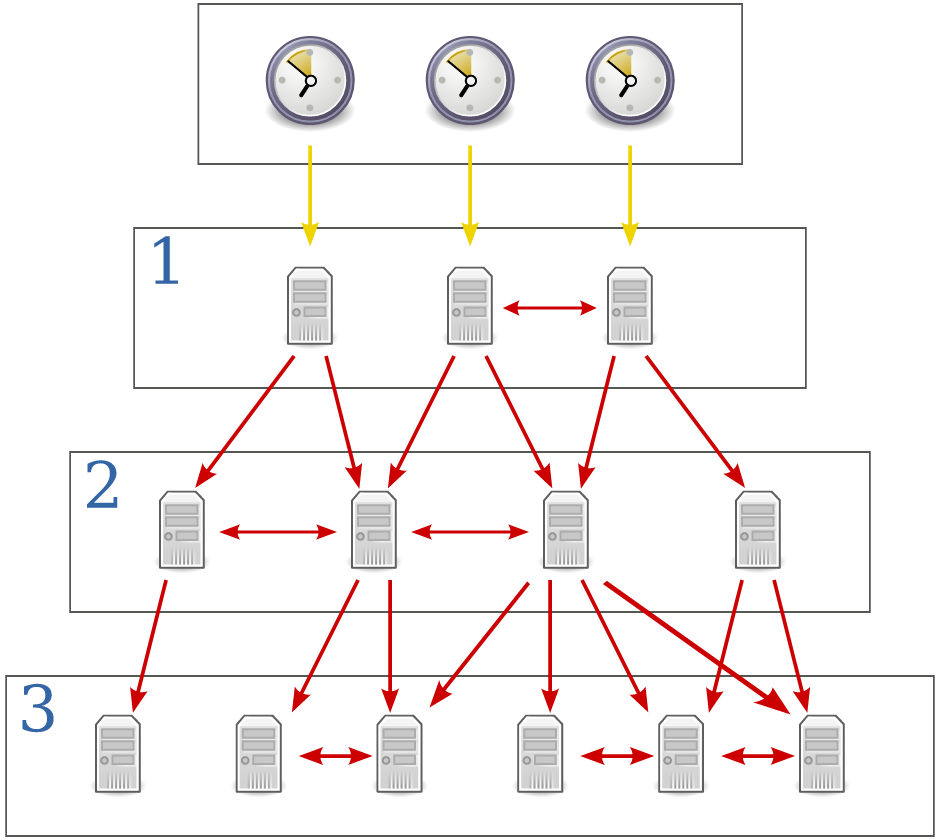
\includegraphics[width=\linewidth]{
      images/theory/Network_Time_Protocol_servers_and_clients.png
    }
    \caption{NTP hierarchy \cite{NetworkTimeProtocol2026}}
  \end{subfigure}
\end{figure}

Il protocollo generalmente opera sopra UDP, sulla porta 123, e utilizza lo
scambio di messaggi timestamp per stimare il ritardo di rete e l'offset tra il
clock locale e una sorgente temporale di riferimento.

\subsection{Modalità operative e topologia gerarchica}
Nella specifica vi sono tre varianti del protocollo NTP, rispettivamente simmetrico,
client/server e broadcast. Ognuna di queste varianti è associata a un diverso insieme
di modalità di pacchetto, che sono indicate in un campo specifico all'interno
del pacchetto NTP. \ref{tab:ntp_association_packet_modes}.

\begin{table}[h]
  \centering
  \begin{tabular}{lcc}
    \hline
    \textbf{Association Mode} & \textbf{Assoc. Mode Value} & \textbf{Packet Mode Value} \\
    \hline
    Symmetric Active          & 1                          & 1 or 2                     \\
    Symmetric Passive         & 2                          & 1                          \\
    Client                    & 3                          & 4                          \\
    Server                    & 4                          & 3                          \\
    Broadcast Server          & 5                          & 5                          \\
    Broadcast Client          & 6                          & N/A                        \\
    \hline
  \end{tabular}
  \caption{Association and packet modes in NTP.}
  \label{tab:ntp_association_packet_modes}
\end{table}

Nella v

Nella variante \texttt{client/server}, un client persistente invia pacchetti di modalità
4 a un server, che restituisce pacchetti di modalità 3. I server forniscono
sincronizzazione a uno o più client, ma non accettano sincronizzazione da loro.
Un server può anche essere un driver di orologio di riferimento che ottiene il
tempo direttamente da una fonte standard come un ricevitore GPS o un servizio di
modem telefonico. In questa variante,i client estraggono la sincronizzazione dai server.
Variante utilizzata in fase di testing, in entrambi le implementazioni NTPsec \ref{NTPsec}
e Chrony \ref{Chrony}.

Nella modalità \texttt{symmetric} due nodi operano come peer. Ciascun peer può trattare
l'altro come potenziale sorgente temporale e la relazione non è strutturata secondo
una direzione gerarchica client--server. Questa modalità è adatta a scenari in cui
più server temporali cooperano tra loro come nodi di pari livello.

La modalità \texttt{broadcast} prevede infine che un server invii periodicamente
messaggi temporali destinati a più client. I client possono ricevere passivamente
tali aggiornamenti, eventualmente dopo una fase iniziale di calibrazione del
ritardo. Questa modalità è utile quando si vuole distribuire la sincronizzazione a
più nodi riducendo lo scambio individuale di messaggi.

Il livello ricoperto da ciascun server nella gerarchia è definito secondo una numerazione
di stratum. Partendo da stratum 1, associato a server primari, si può arrivare
ad un massimo di 15 (16 si considera non sincronizzato). All'aumentare del numero
di stratum, la sua precisione si degrada a seconda del percorso di rete
specifico e della stabilità dell'orologio di sistema. Gli errori medi, misurati
in base alle distanze di sincronizzazione, aumentano approssimativamente in proporzione
ai numeri di stratum e al ritardo di andata e ritorno misurato.

NTP organizza la sincronizzazione secondo una struttura gerarchica orientata a evitare
cicli e a minimizzare la distanza di sincronizzazione rispetto alle sorgenti primarie.
La RFC 5905 descrive tale organizzazione come basata su una variante dell'algoritmo
distribuito Bellman-Ford, utilizzata per determinare uno spanning tree dei percorsi
più brevi radicato sui primary server~ \cite{martinNetworkTimeProtocol2010} In
questo modo, la subnet NTP può riorganizzarsi automaticamente in presenza di guasti
o variazioni nella rete temporale.

-------------
\subsection{Stima di offset e delay}
Il tempo di sistema è rappresentato dall'orologio di sistema gestito dall'hardware
e dal sistema operativo. L'obiettivo degli algoritmi NTP è minimizzare sia la
differenza di tempo che la differenza di frequenza tra UTC (Coordinated Universal
Time, o l'orologio di riferimento) e l'orologio di sistema. Quando queste
differenze sono state ridotte al di sotto delle tolleranze nominali, si dice che l'orologio
di sistema è sincronizzato con UTC. Un timestamp $T(t)$ rappresenta la data UTC
o l'offset di tempo rispetto a UTC al tempo di esecuzione t. Il significato inteso
dovrebbe essere chiaro dal contesto. Sia $T(t)$ l'offset di tempo, $R(t)$ l'offset
di frequenza e $D(t)$ il tasso di invecchiamento (derivata prima di $R(t)$
rispetto a t). Quindi, se $T(t_{0})$ è lo scostamento temporale UTC determinato a
$t = t_{0}$, lo scostamento temporale UTC al tempo t è

\[
  T(t) = T(t_{0}) + R(t_{0})(t-t_{0}) + 1/2 * D(t_{0})(t-t_{0})^{2}+ e
\]

dove e è un termine di errore stocastico.

Quattro statistiche vengono aggiornate ogni volta che un client effettua una
misurazione con un server. Lo scomostamento, ossia il \texttt{theta}, è
rappresentazione dello scostamento temporale di massima verosimiglianza dell'orologio
del server rispetto all'orologio di sistema. Vi è poi il ritardo,definito come \texttt{delta},
che è definito come il ritardo di andata e ritorno tra client e server. Vi è poi
la dispersione, \texttt{epsilon} cioè l'errore massimo intrinseco alla
misurazione, la quale aumenta a una velocità pari alla massima tolleranza di frequenza
dell'orologio di sistema disciplinato $PHI$, tipicamente 15 ppm. Infine, il
jitter, definito come \texttt{psi}, è la media quadratica (RMS) delle differenze di
offset più recenti e rappresenta l'errore nominale nella stima dell'offset.

La specifica NTPv4 descrive inoltre il protocollo come un insieme di processi e strutture
di stato, distinguendo tra variabili associate ai pacchetti, allo stato dei peer,
al processo di polling, allo stato di sistema e alla disciplina del clock \cite{martinNetworkTimeProtocol2010}.
Questa organizzazione evidenzia che il demone non si limita a ricevere timestamp
e applicare una correzione immediata, ma mantiene informazioni sullo stato delle associazioni,
valuta la qualità delle sorgenti e utilizza tali informazioni nel processo di
selezione, filtraggio e correzione del clock locale.

Dal punto di vista dei dati scambiati, un pacchetto NTP contiene informazioni
relative sia allo stato della sorgente temporale sia ai timestamp necessari alla
stima del tempo. Tra i campi più rilevanti per l'analisi della sincronizzazione vi
sono \texttt{mode}, che identifica la modalità del pacchetto, \texttt{stratum},
che indica la distanza gerarchica dalla sorgente di riferimento, \texttt{poll}, che
descrive l'intervallo di interrogazione, \texttt{rootdelay} e \texttt{rootdisp}, che
rappresentano rispettivamente il ritardo e la dispersione cumulativi verso la sorgente
primaria, e \texttt{refid}, che identifica il riferimento temporale utilizzato. Il
pacchetto include inoltre i timestamp \texttt{org}, \texttt{rec}, \texttt{xmt} e
\texttt{dst}, corrispondenti ai quattro istanti utilizzati nel modello di stima
di delay e offset. \cite{martinNetworkTimeProtocol2010}

Dal punto di vista del formato dei messaggi, un pacchetto NTP è trasportato come datagramma
UDP e contiene un header composto da campi che descrivono sia lo stato della sorgente
temporale sia i timestamp utilizzati per la stima della sincronizzazione \cite{martinNetworkTimeProtocol2010}.

Dal punto di vista del trasporto, NTP opera tramite pacchetti scambiati su UDP, tipicamente
sulla porta 123. La scelta di UDP è coerente con la natura della sincronizzazione
temporale: il protocollo non richiede consegna affidabile dei messaggi, poiché eventuali
ritrasmissioni introdurrebbero ulteriore ritardo e renderebbero meno rappresentativa
l'informazione temporale trasportata dal pacchetto. La RFC 5905 osserva infatti
che un trasporto affidabile, come TCP, può risultare controproducente per NTP, in
quanto i retry aumenterebbero il delay e gli errori associati alla stima temporale
\cite{martinNetworkTimeProtocol2010}.

Il protocollo on-wire si basa quindi sullo scambio di datagrammi contenenti timestamp
e informazioni di stato. Tali timestamp consentono di stimare il round-trip
delay e l'offset tra client e sorgente temporale. Ne consegue che la qualità della
sincronizzazione dipende direttamente dalle condizioni del percorso di rete:
delay variabile, jitter, perdita di pacchetti e congestione possono alterare la
regolarità delle osservazioni disponibili al demone.

\subsection{Filtraggio, selezione e disciplina del clock}
In NTPv4 è presente una sequenza di elaborazione delle osservazioni temporali, al
fine di ridurre l'effetto di misure rumorose, selezionare sorgenti coerenti e
correggere il clock del sistema in modo controllato
\cite{martinNetworkTimeProtocol2010}.

Il primo livello di elaborazione è il \textit{clock filter algorithm}. Per ogni
associazione con una sorgente temporale, il demone mantiene un insieme di campioni
recenti, ciascuno associato alle misure osservate. L'idea di base è individuare le
osservazioni più affidabili, privilegiando in generale campioni caratterizzati
da minore incertezza. In questo modo, il protocollo evita che una singola misura
degradata produca immediatamente una correzione errata del clock locale.

In seguito al filtraggio delle misure associate ai singoli peer, il demone procede
con il \textit{system process}, che valuta le sorgenti temporali disponibili.
Quando sono presenti più sorgenti, NTP deve stabilire quali siano coerenti tra loro
e quali debbano essere escluse perché considerate inaffidabili o anomale. Il
processo di selezione riduce quindi l'insieme delle sorgenti candidate e
individua il riferimento temporale da utilizzare per la sincronizzazione del
sistema. Anche quando nel testbed è presente una topologia controllata e con poche
sorgenti, questo meccanismo è concettualmente rilevante: la qualità della sorgente
percepita dal demone influenza lo stato operativo e le metriche riportate.

L'ultimo passaggio è la \textit{clock discipline}, cioè il meccanismo mediante il
quale le stime selezionate vengono utilizzate per correggere il clock locale. La
correzione non coincide necessariamente con uno spostamento immediato dell'orologio
di sistema. Il demone può intervenire anche regolando progressivamente la frequenza
di avanzamento del clock, in modo da ridurre l'offset preservando la continuità
temporale. Questa distinzione è importante: una misura di offset rappresenta una
stima dello scostamento, mentre la disciplina del clock determina come tale stima
viene trasformata in una correzione effettiva.

\subsection{NTPsec e il demone ntpd}

NTPsec è un progetto nato con l'obiettivo di fornire una implementazione più
sicura e manutenibile del protocollo NTP, mantenendo la compatibilità con la specifica
RFC 5905. Il progetto si è sviluppato a partire da NTP Classic. L'obiettivo di
NTPsec è quello di offrire una versione più robusta e semplificata del
protocollo, ottenutos anche attraverso la rimozione di codice legacy e funzionalità
obsolete. Questa caratteristica è rilevante soprattutto in contesti in cui il
demone di sincronizzazione è esposto in rete e deve operare come componente
infrastrutturale affidabile \cite{SecureNetworkTime}.

Il componente principale della suite è il demone \texttt{ntpd}, responsabile
dell'esecuzione del servizio NTP sul nodo. Il demone gestisce le associazioni configurate,
comunica con le sorgenti temporali, mantiene lo stato della sincronizzazione e applica
le correzioni necessarie al clock locale. Accanto al demone, la suite fornisce strumenti
di interrogazione e controllo, come \texttt{ntpq}, utilizzabili per osservare lo
stato delle associazioni e le metriche prodotte dal servizio.

\begin{table}[h]
  \centering
  \begin{tabular}{lll}
    \hline
    \textbf{Comando / fonte} & \textbf{Metrica / campo}       & \textbf{Significato}                                           \\
    \hline
    \texttt{ntpq -p}         & \texttt{remote}                & Sorgente o peer NTP remoto configurato.                        \\
    \texttt{ntpq -p}         & \texttt{refid}                 & Identificativo della sorgente temporale di riferimento.        \\
    \texttt{ntpq -p}         & \texttt{st}                    & Stratum della sorgente remota.                                 \\
    \texttt{ntpq -p}         & \texttt{t}                     & Tipo di associazione NTP.                                      \\
    \texttt{ntpq -p}         & \texttt{when}                  & Tempo trascorso dall'ultimo pacchetto ricevuto dalla sorgente. \\
    \texttt{ntpq -p}         & \texttt{poll}                  & Intervallo di polling verso la sorgente.                       \\
    \texttt{ntpq -p}         & \texttt{reach}                 & Registro di raggiungibilità della sorgente.                    \\
    \texttt{ntpq -p}         & \texttt{delay}                 & Ritardo stimato del percorso verso la sorgente.                \\
    \texttt{ntpq -p}         & \texttt{offset}                & Scostamento stimato tra clock locale e sorgente temporale.     \\
    \texttt{ntpq -p}         & \texttt{jitter}                & Variabilità delle misure associate alla sorgente.              \\
    \hline
    \texttt{peerstats}       & \texttt{offset}                & Scostamento stimato rispetto al peer remoto.                   \\
    \texttt{peerstats}       & \texttt{delay}                 & Ritardo stimato dell'associazione con il peer.                 \\
    \texttt{peerstats}       & \texttt{dispersion}            & Incertezza stimata della misura temporale.                     \\
    \texttt{peerstats}       & \texttt{jitter}                & Jitter RMS associato alle misure del peer.                     \\
    \hline
    \texttt{loopstats}       & \texttt{offset}                & Offset del clock locale rispetto alla sorgente selezionata.    \\
    \texttt{loopstats}       & \texttt{frequency}             & Correzione di frequenza applicata al clock locale.             \\
    \texttt{loopstats}       & \texttt{jitter}                & Variabilità stimata del clock locale.                          \\
    \texttt{loopstats}       & \texttt{wander}                & Variabilità lenta della frequenza del clock locale.            \\
    \hline
    \texttt{rawstats}        & \texttt{originate timestamp}   & Timestamp di invio della richiesta da parte del client.        \\
    \texttt{rawstats}        & \texttt{receive timestamp}     & Timestamp di ricezione della richiesta presso il server.       \\
    \texttt{rawstats}        & \texttt{transmit timestamp}    & Timestamp di invio della risposta da parte del server.         \\
    \texttt{rawstats}        & \texttt{destination timestamp} & Timestamp locale di ricezione della risposta presso il client. \\
    \hline
    \texttt{readvar}         & \texttt{rootdelay}             & Ritardo cumulativo verso la sorgente primaria.                 \\
    \texttt{readvar}         & \texttt{rootdisp}              & Dispersione cumulativa verso la sorgente primaria.             \\
    \texttt{readvar}         & \texttt{stratum}               & Livello gerarchico del sistema locale.                         \\
    \texttt{readvar}         & \texttt{refid}                 & Identificativo della sorgente selezionata.                     \\
    \texttt{readvar}         & \texttt{leap}                  & Stato relativo alla sincronizzazione e ai leap second.         \\
    \hline
  \end{tabular}
  \caption{Principali metriche e campi esposti da NTPsec tramite \texttt{ntpd},
  \texttt{ntpq} e file statistici, rielaborati dalla documentazione ufficiale~\cite{ntpsec-doc}.}
  \label{tab:ntpsec_metriche}
\end{table}

\subsection{Chrony e il demone chronyd}
\label{Chrony}

Chrony è una suite software per la sincronizzazione temporale e costituisce una
implementazione versatile del Network Time Protocol. Il progetto è progettato per
sincronizzare il clock di sistema rispetto a server NTP, reference clock, come ricevitori
GPS, oppure input manuali; può inoltre operare come server NTPv4, fornendo
sincronizzazione ad altri nodi della rete~\cite{ChronyDocumentation}.

Dal punto di vista protocollare, Chrony non definisce un protocollo alternativo a
NTP, ma implementa la sincronizzazione basata su NTP con una propria
architettura software e proprie strategie interne di stima e controllo del clock.
Questa distinzione è rilevante nel contesto della tesi, poiché Chrony e NTPsec
appartengono allo stesso ambito protocollare, ma rappresentano implementazioni differenti:
eventuali differenze di comportamento devono quindi essere ricondotte non al
protocollo di riferimento, bensì alle scelte implementative e operative dei rispettivi
demoni.

La suite Chrony è composta principalmente da due programmi: \texttt{chronyd} e \texttt{chronyc}.
Il primo è il demone responsabile della sincronizzazione del clock locale e viene
normalmente eseguito come servizio di sistema. Il secondo è un'interfaccia a
riga di comando che consente di interrogare lo stato del demone, monitorarne le prestazioni
e modificare alcuni parametri operativi durante l'esecuzione \cite{ChronyDocumentation}.

Una caratteristica rilevante di Chrony è la sua progettazione orientata al funzionamento
in condizioni operative variabili. La documentazione del progetto evidenzia
infatti il supporto a scenari quali connessioni di rete intermittenti, reti congestionate,
variazioni di temperatura che influenzano il clock locale, sistemi non sempre attivi
e ambienti virtualizzati \cite{ChronyDocumentation}. Queste caratteristiche
rendono Chrony particolarmente adatto a contesti nei quali la sincronizzazione
deve rimanere efficace anche quando la disponibilità della sorgente temporale o
la qualità del percorso di rete non sono costanti.

Le metriche rese disponibili da Chrony, in particolare attraverso le informazioni
di \textit{tracking} e \textit{sourcestats}, permettono di osservare lo stato
del clock locale, la qualità della sorgente temporale e la variabilità delle misure
utilizzate dal demone.

\begin{table}[h]
  \centering
  \begin{tabular}{lll}
    \hline
    \textbf{Comando / fonte} & \textbf{Metrica / campo} & \textbf{Significato}                                                         \\
    \hline
    \texttt{tracking}        & \texttt{Reference ID}    & Identificativo della sorgente selezionata.                                   \\
    \texttt{tracking}        & \texttt{Stratum}         & Livello gerarchico del nodo rispetto alla sorgente primaria.                 \\
    \texttt{tracking}        & \texttt{Ref time}        & Istante dell'ultimo aggiornamento dal riferimento.                           \\
    \texttt{tracking}        & \texttt{System time}     & Scostamento residuo del clock di sistema rispetto al tempo stimato corretto. \\
    \texttt{tracking}        & \texttt{Last offset}     & Ultimo offset misurato rispetto alla sorgente selezionata.                   \\
    \texttt{tracking}        & \texttt{RMS offset}      & Valore quadratico medio degli offset recenti.                                \\
    \texttt{tracking}        & \texttt{Frequency}       & Correzione di frequenza applicata al clock locale.                           \\
    \texttt{tracking}        & \texttt{Residual freq}   & Frequenza residua stimata dopo la correzione.                                \\
    \texttt{tracking}        & \texttt{Skew}            & Incertezza nella stima della frequenza del clock.                            \\
    \texttt{tracking}        & \texttt{Root delay}      & Ritardo cumulativo verso la sorgente primaria.                               \\
    \texttt{tracking}        & \texttt{Root dispersion} & Dispersione cumulativa verso la sorgente primaria.                           \\
    \texttt{tracking}        & \texttt{Update interval} & Intervallo tra gli ultimi aggiornamenti della sincronizzazione.              \\
    \texttt{tracking}        & \texttt{Leap status}     & Stato relativo alla sincronizzazione e ai leap second.                       \\
    \hline
    \texttt{sources}         & \texttt{MS}              & Tipo e stato della sorgente temporale.                                       \\
    \texttt{sources}         & \texttt{Name/IP address} & Nome o indirizzo della sorgente.                                             \\
    \texttt{sources}         & \texttt{Stratum}         & Stratum dichiarato dalla sorgente.                                           \\
    \texttt{sources}         & \texttt{Poll}            & Intervallo di polling verso la sorgente.                                     \\
    \texttt{sources}         & \texttt{Reach}           & Registro di raggiungibilità della sorgente.                                  \\
    \texttt{sources}         & \texttt{LastRx}          & Tempo trascorso dall'ultimo campione ricevuto.                               \\
    \texttt{sources}         & \texttt{Last sample}     & Ultimo offset misurato rispetto alla sorgente.                               \\
    \hline
    \texttt{sourcestats}     & \texttt{NP}              & Numero di campioni mantenuti per la sorgente.                                \\
    \texttt{sourcestats}     & \texttt{NR}              & Numero di run dei residui con lo stesso segno.                               \\
    \texttt{sourcestats}     & \texttt{Span}            & Intervallo temporale coperto dai campioni.                                   \\
    \texttt{sourcestats}     & \texttt{Frequency}       & Frequenza stimata rispetto alla sorgente.                                    \\
    \texttt{sourcestats}     & \texttt{Freq Skew}       & Incertezza della stima di frequenza.                                         \\
    \texttt{sourcestats}     & \texttt{Offset}          & Offset stimato della sorgente.                                               \\
    \texttt{sourcestats}     & \texttt{Std Dev}         & Deviazione standard dei residui delle misure.                                \\
    \hline
  \end{tabular}
  \caption{Principali metriche e campi esposti da Chrony tramite \texttt{chronyc}.}
  \label{tab:chrony_metriche}
\end{table}

\section{Precision Time Protocol}
\subsection{Caratteristiche generali di PTP}
\subsection{linuxptp e il demone ptp4l}

\section{Motivazione della scelta degli strumenti analizzati}
  \chapter{Ambiente sperimentale}
\label{cha:ambienteSperimentale}

\section{Obiettivo e criteri di progettazione del testbed}

L'Obiettivo di base per la progettazione del testbed è quello di creare un ambiente
controllato, riproducibile e parametrizzabile all'interno del quale poter
valutare il differente comportamento dei demoni di sincronizzazione temporale in
condizioni di rete variabili. Nel caso in questione: linuxptp, chrony e ntpsec.
L'impostazione è stata scelta per mettere in evidenza non la precisione assoluta
dei nodi rispetto a una sorgente temporale esterna, quindi con un riferimento UTC,
ma la loro capacità nel mantenere una relazione temporale coerente all'interno
dell'ambiente sperimentale, al differire delle condizioni dei canali di comunicazione.

L'ambiente si basa su tre criteri fondamentali. Per primo bisogna isolare
completamente il testbed dalla rete esterna. Non essendoci necessità di riferimenti
esterni è stato possibile disabilitare ogni forma di connettività, garantendo il
massimo isolamento e costringendo i nodi a sincronizzarsi all'interno della sola
topologia di rete. Il secondo criterio è stato la riproducibilità dell'ambiente.
Infine l'ultimo ciriterio coinvolgeva la parametrizzazione degli impairment di
rete, i quali devono essere facilmetne modificabili, potendo gestire in modo
indipendente da ogni script la loro applicazione.

La topolgia è stata creata con l'utilizzo dei container Docker. I rami logici sono
stati opportunamenti separati e lo stesso ragionamento è stato applicato agli script,
con l'obiettivo di ridurre al minimo interferenze tra demoni e protocolli
differenti. Le condizioni di rete sono state modificate mediante l'utilizzo di Linux
Traffic Control.

\section{Topologia di rete}
La topologia si divide su due reti logiche sperate, rappresentative dell'evoluzione
della topologia T1, utilizzata per la fase di test preliminari, ma poi risultata
obsoleta. La rete A è stata associata a una subnet \texttt{10.0.10.0/24}, mentre la
rete B è stata associata ad una subnet \texttt{10.0.20.0/24}. I nodi \texttt{servergm},
\texttt{serverntp}, \texttt{clientchrony} e l'interfaccia \texttt{eth0} di \texttt{boundary}
sono stati collocati nella rete A, mentre \texttt{clientptp}, \texttt{clientntp}
e l'interfaccia \texttt{eth1} di\texttt{boundary} sono stati collocati nella rete
B. La scelta si basa sulla praticità operativa, si è cercato di evitare i conflitti
di configurazioni tra demoni e protocolli differenti, raccogliendo al meglio, sucessivamente,
i dati.

Il nodo \texttt{boundary} è stato configurato come nodo intermedio tra le due reti
assumendo un differente ruolo al variare del demone considerato. Nel caso di PTP,
assume un ruolo di boundary clock ricevendo sincronizzazione dalla rete A e propagandola
verso la rete B, mentrenel caso di NTPsec, è utilizzato come nodo intermedio tra \texttt{serverntp}
e \texttt{clientntp}. Per Chrony non è stato necessario il suo utilizzo.

{ \setlength{\intextsep}{8pt} \setlength{\textfloatsep}{8pt} \setlength{\floatsep}{8pt}

\begin{table}[H]\captionsetup{skip=4pt} \begin{tabular}{lll}\hline \textbf{Nodo} & \textbf{Rete} & \textbf{Ruolo sperimentale} \\ \hline \texttt{servergm} & A & Sorgente interna per PTP e Chrony \\ \texttt{serverntp} & A & Sorgente interna per NTPsec \\ \texttt{boundary} & A / B & Nodo intermedio; boundary clock PTP \\ \texttt{clientptp} & B & Nodo client PTP \\ \texttt{clientntp} & B & Nodo client NTPsec \\ \texttt{clientchrony} & A & Nodo client Chrony \\ \hline\end{tabular} \caption{Nodi della topologia T2 e ruoli assegnati nel testbed.} \label{tab:nodi_t2}\end{table}

\vspace{1cm}

\begin{figure}[H]\centering \begin{tikzpicture}[ node distance=1.5cm and 1.8cm, box/.style={ rectangle, draw, rounded corners, align=center, minimum width=3.8cm, minimum height=1.25cm, font=\small }, netbox/.style={ rectangle, draw, rounded corners, inner sep=0.45cm, fill=gray!8 }, arrow/.style={ -{Latex[length=3mm]}, thick }, edgeLabel/.style={ midway, fill=white, inner sep=1pt, font=\footnotesize } ]
% --- Nodi rete A ---
\node[box] (servergm) {%
\texttt{servergm}\\ Grandmaster PTP / Server Chrony\\ \texttt{eth0: 10.0.10.1} };

\node[box, right=2.2cm of servergm] (serverntp) {%
\texttt{serverntp}\\ Server NTPsec\\ \texttt{eth0: 10.0.10.4} };

\node[box, below=1.5cm of servergm] (clientchrony) {%
\texttt{clientchrony}\\ Client Chrony\\ \texttt{eth0: 10.0.10.3} };

\node[box, below=1.5cm of serverntp] (boundary) {%
\texttt{boundary}\\ Boundary Clock / nodo intermedio\\ \texttt{eth0: 10.0.10.2}\\ \texttt{eth1: 10.0.20.1} };


% --- Nodi rete B ---
\node[box, below=3.0cm of boundary, xshift=-2.2cm] (clientntp) {%
\texttt{clientntp}\\ Client NTPsec\\ \texttt{eth0: 10.0.20.2} };

\node[box, below=3.0cm of boundary, xshift=2.2cm] (clientptp) {%
\texttt{clientptp}\\ Client PTP\\ \texttt{eth0: 10.0.20.3} };


% --- Domini/reti ---
\begin{scope}[on background layer]\node[netbox, fit=(servergm)(serverntp)(clientchrony)(boundary)] (domainA) {};

\node[netbox, fit=(clientntp)(clientptp)] (domainB) {};\end{scope}


% --- Titoli domini ---
\node[font=\bfseries, above=0.15cm of domainA.north] {Rete A -- \texttt{10.0.10.0/24}};

\node[font=\bfseries, above=0.15cm of domainB.north] {Rete B -- \texttt{10.0.20.0/24}};


% --- Collegamenti logici ---
\draw[arrow] (servergm) -- node[edgeLabel] {Chrony} (clientchrony); \draw[arrow] (servergm) -- node[edgeLabel] {PTP} (boundary); \draw[arrow] (serverntp) -- node[edgeLabel] {NTPsec} (boundary); \draw[arrow] (boundary) -- node[edgeLabel, left] {NTPsec} (clientntp); \draw[arrow] (boundary) -- node[edgeLabel, right] {PTP} (clientptp);\end{tikzpicture} \caption{Topologia logica T2 utilizzata nel testbed sperimentale. La rete A ospita le sorgenti temporali interne e il client Chrony, mentre la rete B ospita i client PTP e NTPsec. Il nodo \texttt{boundary} collega le due reti tramite le interfacce \texttt{eth0} e \texttt{eth1}.} \label{fig:topologia_t2}\end{figure}

\vspace{0.4cm} }

Per ragioni configurative, si è reso necessario spearare la sorgente temporale
in due nodi differenti, distinguendo tra PTP e Chrony da un lato, e NTPsec dall'altro.
Conflitti di configurazione, installazione e permessi rendevano incompatibile l'installazione
di implementazioni software differenti sullo stesso nodo, soprattutto nei casi in
cui più servizi potevano tentare di intervenire sullo stesso clock locale.Inoltre
la separazione logica delle rete permette di avere una distinzione più chiara tra
le diverse catene di sincronizzazione analizzate nel testbed.

\section{Ambiente containerizzato}

Il testbed è realizzato tramite la creazione di una topologia di rete
containerizzata attraverso l'ausilio di Kathará, cioè un sisteama di emulazione di
rete open source basato su container. Questa scelta ha reso possibile la
riproduzione di una rete composta da un insieme di nodi Linux isolati, ognuno dotato
di una sua interfaccia, di file di configurazioni personalizzati e degli
specifici demoni di sincronizzazione. L'utilizzo dei container ha permesso inoltre
di automatizzare l'intero ciclo sperimentale, rendendo possibile l'inizializzazione
della topologia, la configuazione degli indirizzi IP, l'installazione dei
pacchetti necessari, la copia dei file di configurazione, l'avvio dei demoni, l'applicazione
degli impairment di rete e infine la raccolta dei log.

Ogni run può essere eseguita a partire da uno stato pulito della topologia,
riducendo il rischio che processi residui, configurazioni di rete precedenti o discipline
di coda già applicate influenzino le misurazioni successive.

\subsection{Kathará e organizzazione dei container}

La topologia T2 viene descritta nel file \texttt{lab.conf}, dove vengono
definiti i nodi del testbed, le differenti reti virtuali a cui essi appartengono,
i volumi condivisi montati all'interno dei container e le capability necessarie
all'esecuzione degli esperimenti.

Nella topologia, descritta come T2, i nodi sono associati a due reti logiche
distinte, indicate come rete A e rete B. I nodi \texttt{servergm}, \texttt{serverntp},
\texttt{clientchrony} e l'interfaccia \texttt{eth0} di \texttt{boundary} appartengono
alla rete A. I nodi \texttt{clientntp}, \texttt{clientptp} e l'interfaccia \texttt{eth1}
di \texttt{boundary} appartengono alla rete B. Il nodo \texttt{boundary} è l'unico
container connesso a entrambe le reti interne e costituisce il punto di interconnessione
tra i due domini.

\begin{lstlisting}[language=bash,caption={Estratto del file \texttt{lab.conf}: assegnazione dei nodi alle reti A e B.},label={lst:labconf_topologia}]

# Topologia T2

servergm[0]=A
serverntp[0]=A
boundary[0]=A
boundary[1]=B
clientchrony[0]=A
clientntp[0]=B
clientptp[0]=B
\end{lstlisting}

Nella fase iniziale di avvio, ogni contanier va ad eseguire il proprio file di inizializzazione
\texttt{.startup}. Essi contengono gli indirizzi IP delle interfacce, attivano i
link, popolano il file \texttt{/etc/hosts}, installano i pacchetti necessari e copiano
i file di configurazione dei demoni dalle directory condivise del progetto verso i
percorsi attesi dal sistema.

Nel nodo \texttt{boundary}, per esempio, si configurano due interfacce interne: \texttt{eth0}
sulla rete A e \texttt{eth1} sulla rete B.

\begin{lstlisting}[language=bash,caption={Estratto di \texttt{boundary.startup}: configurazione delle interfacce interne.},label={lst:boundary_startup_ip}]
ip addr add 10.0.10.2/24 dev eth0
ip addr add 10.0.20.1/24 dev eth1
ip link set eth0 up
ip link set eth1 up
\end{lstlisting}

Per quanto riguarda la risoluzione locale dei nomi, ogni nodo mantiene un file \texttt{/etc/hosts}
che associa gli hostname ai rispettivi indirizzi IP, evitando problematiche derivate
dalla dipendenza da servizi DNS esterni e rende esplicita la corrispondenza tra hostname
e indirizzi IP della topologia.

\begin{lstlisting}[language=bash,caption={Mappatura locale degli hostname nei container.},label={lst:hosts_mapping}]
10.0.10.1 servergm
10.0.10.4 serverntp
10.0.10.2 boundary0
10.0.20.1 boundary1
10.0.10.3 clientchrony
10.0.20.2 clientntp
10.0.20.3 clientptp
\end{lstlisting}

Distinguendo tra \texttt{boundary0} e \texttt{boundary1} si riesce a
identificare in modo chiaro le due interfacce del nodo \texttt{boundary}.
\texttt{boundary0} corrisponde all'interfaccia sulla rete A (\texttt{10.0.10.2}),
mentre \texttt{boundary1} corrisponde all'interfaccia sulla rete B (\texttt{10.0.20.1}).
Ciò è utile ai fini del testNTPsec, nei quali il nodo \texttt{clientntp}
utilizza il boundary come sorgente temporale raggiungibile sulla rete B.

All'interno del file \texttt{lab.conf} viene montata una directory del progetto all'interno
di tutti i container. Tale volume condiviso viene utilizzato sia per rendere
accessibili i file di configurazione ai nodi, sia per salvare i log prodotti durante
le run sperimentali.

\begin{lstlisting}[language=bash,caption={Estratto del file \texttt{lab.conf}: volume condiviso tra host e container.},label={lst:labconf_volume}]
servergm[volume]=/home/gabrielemenestrina/tesi_sync_lab|/tesi_sync_lab|rw
serverntp[volume]=/home/gabrielemenestrina/tesi_sync_lab|/tesi_sync_lab|rw
boundary[volume]=/home/gabrielemenestrina/tesi_sync_lab|/tesi_sync_lab|rw
clientchrony[volume]=/home/gabrielemenestrina/tesi_sync_lab|/tesi_sync_lab|rw
clientntp[volume]=/home/gabrielemenestrina/tesi_sync_lab|/tesi_sync_lab|rw
clientptp[volume]=/home/gabrielemenestrina/tesi_sync_lab|/tesi_sync_lab|rw
\end{lstlisting}

L'obiettivo alla base di tale scelta è duplice. Se da un lato permette di mantenere
tutti i file di configurazione all'interno della repository del progetto e copirali
nei differenti container in fase di avvio, allo stesso modo consente ai demoni e
agli script di scrivere i log in una directory persistente accessibile dall'host,
evitando problematicità dovute alla chiusura della topologia.

Ad esempio, il nodo \texttt{servergm} installa Chrony e linuxptp, copia la
configurazione Chrony lato server e predispone il file di configurazione PTP da
utilizzare come grandmaster interno del dominio sperimentale.

\begin{lstlisting}[language=bash,caption={Estratto di \texttt{servergm.startup}: installazione e copia delle configurazioni.},label={lst:servergm_startup}]
apt update -y
apt install -y chrony linuxptp

cp /tesi_sync_lab/configs/chrony/server_chrony.conf /etc/chrony/chrony.conf

pkill chronyd 2>/dev/null
sleep 2
chronyd &

mkdir -p /etc/ptp
cp /tesi_sync_lab/configs/ptp/server_ptp.conf /etc/ptp/server_gm.conf
\end{lstlisting}

Analogamente, il nodo \texttt{clientchrony} installa Chrony, copia la
configurazione client e avvia manualmente il demone \texttt{chronyd}. La scelta
dell'avvio manuale è stata preferita poichè, all'interno dei container, la
gestione tramite \texttt{systemctl} non è necessaria e può risultare meno adatta rispetto
all'avvio diretto del processo.

\begin{lstlisting}[language=bash,caption={Estratto di \texttt{clientchrony.startup}: configurazione e avvio del client Chrony.},label={lst:clientchrony_startup}]
apt update -y
apt install -y chrony

cp /tesi_sync_lab/configs/chrony/client_chrony.conf /etc/chrony/chrony.conf

pkill chronyd 2>/dev/null
sleep 2
chronyd &
\end{lstlisting}

In NTPsec, il nodo \texttt{serverntp} installa il pacchetto \texttt{ntpsec},
copia la configurazione server e avvia \texttt{ntpd}. Una procedura simile viene
adottata per il nodo\texttt{clientntp} che però utilizza una confiurazione lato
client. Per quanto riguarda invece il nodo \texttt{boundary} si ha sia la
configurazione PTP sia la configurazione NTPsec, ma i demoni non vengono mantenuti
attivi simultaneamente in quanto potrebbero essere causa di conflitti interni,
come problematicità di permessi.

\begin{lstlisting}[language=bash,caption={Estratto di \texttt{serverntp.startup}: configurazione e avvio di NTPsec.},label={lst:serverntp_startup}]
apt update -y
apt install -y ntpsec

cp /tesi_sync_lab/configs/ntp/server_ntp.conf /etc/ntpsec/ntp.conf

pkill ntpd 2>/dev/null
sleep 2
/usr/sbin/ntpd -g -c /etc/ntpsec/ntp.conf &
\end{lstlisting}

Il nodo \texttt{clientptp} installa invece \texttt{linuxptp} e copia il file di configurazione
PTP lato client. L'avvio effettivo del demone \texttt{ptp4l} non avviene direttamente
nel file \texttt{.startup}, ma viene gestito successivamente dagli script di esecuzione,
in modo da controllare l'ordine di avvio del grandmaster, del boundary clock e del
client PTP.

\begin{lstlisting}[language=bash,caption={Estratto di \texttt{clientptp.startup}: predisposizione della configurazione PTP lato client.},label={lst:clientptp_startup}]
apt update -y
apt install -y linuxptp

mkdir -p /etc/ptp
cp /tesi_sync_lab/configs/ptp/client_ptp.conf /etc/ptp/client_ptp.conf
\end{lstlisting}

Uno script differente, indicato come \texttt{bootstrapT3\_V2.sh}, viene utilizzato
per coordinare l'intera esecuzione sperimentale. Esso definisce gli scenari da
eseguire, l'insieme delle run, la directory di output dei log, il percorso della topologia
Kathará e l'interfaccia su cui applicare gli impairment per i test che perturbano
il ramo B.

\begin{lstlisting}[language=bash,caption={Variabili principali dello script \texttt{bootstrapT3\_V2.sh}.},label={lst:bootstrap_vars}]
SCENARIOS=("low" "medium" "high")
SCENARIO_DIR="$(dirname "$0")/scenarios"
RAWLOG_ROOT="analysis/raw_logs/T3_multiplerun"
NETNS="boundary"
IFACE="eth1"   # boundary lato rete B
TOPOLOGY_DIR="topologies/T2"

RUNS=15

mkdir -p "$RAWLOG_ROOT"
\end{lstlisting}

Ogni scenario viene eseguito più volte. Nel caso mostrato, per ciascuno scenario
sono previste quindici run indipendenti. Permettendo di ridurre eventuali rumori statistici
e di ottenere una distribuzione più affidabile dei risultati.

\subsection{Privilegi e capability}

Ogni esecuzione dei demoni di sincronizzazione richiede specifici privilegi all'interno
dei container, e lo stesso accade per l'applicazione degli impairment di rete introdotti,
da qui nasce la necessità di avviare in modalità privilegiata la topologia e di
assegnare capability aggiuntive ai nodi, \texttt{--privileged}. Così facendo si sono
ridotti problemi leagti alle restrizioni imposte dal runtime dei container.

Le capacibility sono un meccanismo del kernel Linux che consente di concedere privilegi
specifici a processi o container senza dover concedere loro l'accesso completo come
utente root. Di seguito sono riportate le capability principali utilizzate nel
testbed: \texttt{SYS\_TIME}, \texttt{NET\_RAW} e \texttt{NET\_ADMIN}.

\begin{lstlisting}[language=bash,caption={Estratto del file \texttt{lab.conf}: capability assegnate ai container.},label={lst:labconf_capabilities}]
clientptp[cap_add]=SYS_TIME,NET_RAW,NET_ADMIN
boundary[cap_add]=SYS_TIME,NET_RAW,NET_ADMIN
servergm[cap_add]=SYS_TIME,NET_RAW,NET_ADMIN
serverntp[cap_add]=SYS_TIME,NET_RAW,NET_ADMIN
clientchrony[cap_add]=SYS_TIME,NET_RAW,NET_ADMIN
\end{lstlisting}

\texttt{SYS\_TIME} consente processi nel container di intervenire sull'orologio di
sistema, questo indipendentemente se poi avviene o meno. Si è reso necessario l'aggiunta
di essa poiché era origine di conflitti internii, in quanto essa è necessaria
per i demoni che disciplinano il clock locale, come \texttt{chronyd}, \texttt{ntpd}
e \texttt{ptp4l}. La capability \texttt{NET\_ADMIN} è necessaria per operazioni amministrative
sulle interfacce di rete, tra cui l'applicazione di qdisc tramite \texttt{tc}.
La capability \texttt{NET\_RAW} abilita invece funzionalità legate all'uso di socket
raw e operazioni di rete richieste da alcuni strumenti o implementazioni.

\begin{lstlisting}[language=bash,caption={Avvio privilegiato della topologia nello script di automazione.},label={lst:kathara_privileged}]
sudo -v
printf 'n\n' | sudo -n kathara lstart -d "$TOPOLOGY_DIR" --privileged
\end{lstlisting}

Nella fase di testbed la topologia viene "ripulita" e riavviata prima di ogni
scenario o run. È stato effettuato tramite \texttt{kathara lclean} elimnando i
container della run precedente, evitando che processi attivi, configurazioni
residue o discipline di coda rimangano applicate all'esecuzione successiva.

\begin{lstlisting}[language=bash,caption={Reset della topologia prima dell'avvio di una run.},label={lst:kathara_lclean}]
kathara lclean -d "$TOPOLOGY_DIR" || true
sudo -v
printf 'n\n' | sudo -n kathara lstart -d "$TOPOLOGY_DIR" --privileged
\end{lstlisting}

L'uso di \texttt{|| true} impedisce che un eventuale errore nella fase di
pulizia, ad esempio dovuto all'assenza di una topologia già attiva, interrompa
lo script.

Un'ulteriore precauzione riguarda l'esecuzione dei demoni sul nodo \texttt{boundary}.
Poiché tale nodo può essere coinvolto sia nei test PTP sia nei test NTPsec, gli script
evitano di mantenere attivi contemporaneamente demoni che potrebbero tentare di disciplinare
lo stesso clock locale. Nel caso PTP, prima dell'avvio di \texttt{ptp4l} sul
grandmaster viene terminato \texttt{chronyd}; nel caso NTPsec, \texttt{ntpd}
viene avviato soltanto quando necessario e con PTP non attivo.

\begin{lstlisting}[language=bash,caption={Esempio di avvio controllato dei demoni PTP.},label={lst:ptp_start_sequence}]
kathara exec -d "$TOPOLOGY_DIR" servergm -- bash -lc 
"pkill chronyd 2>/dev/null || true; 
sleep 1; 
ptp4l -f /etc/ptp/server_gm.conf -m -i eth0 -S 
&> /tesi_sync_lab/$RUN_DIR/ptp_server.log &"

sleep 3

kathara exec -d "$TOPOLOGY_DIR" boundary -- bash -lc 
"ptp4l -f /etc/ptp/bc.conf -m -i eth0 -i eth1 -S 
&> /tesi_sync_lab/$RUN_DIR/ptp_boundary.log &"

sleep 3

kathara exec -d "$TOPOLOGY_DIR" clientptp -- bash -lc 
"ptp4l -f /etc/ptp/client_ptp.conf -m -i eth0 -S -s 
&> /tesi_sync_lab/$RUN_DIR/ptp_client.log &"
\end{lstlisting}

La sequenza di avvio è rilevante perché permette di inizializzare prima il grandmaster,
poi il boundary clock e infine il client PTP. In questo modo, il dominio PTP
viene costruito secondo la gerarchia attesa, riducendo la presenza di transitori dovuti
all'assenza iniziale di una sorgente temporale.

\subsection{Isolamento dalla rete esterna}

Nella fase di avvio si è reso necessario mantenere la connettività verso l'esterno
per consentire l'installazione dei pacchetti necessari, quali \texttt{chrony}, \texttt{ntpsec}
e \texttt{linuxptp}, e l'aggiornametno delle repository. Questo spiega la presenza
di bridge temporanei verso l'esterno, che vengono successivamente disabilitati
per garantire l'isolamento del testbed.

\begin{lstlisting}[language=bash,caption={Estratto del file \texttt{lab.conf}: bridge temporaneo verso l'esterno.},label={lst:labconf_bridged}]
servergm[bridged]=true
serverntp[bridged]=true
boundary[bridged]=true
clientchrony[bridged]=true
clientntp[bridged]=true
clientptp[bridged]=true
\end{lstlisting}

Successivamente, terminata l'inzializzazione della T2, la connettività esterna è stata
disabilitata utilizzando lo script \texttt{endInternetConnection.sh}.

Lo script disabilita l'interfaccia esterna sui nodi dotati di una sola
interfaccia interna e disabilita l'interfaccia esterna dedicata sul nodo \texttt{boundary}.
Nei nodi collegati a una sola rete interna, l'interfaccia \texttt{eth0} è
utilizzata per la topologia sperimentale, mentre \texttt{eth1} rappresenta l'interfaccia
bridged verso l'esterno. Nel nodo \texttt{boundary}, invece, \texttt{eth0} ed \texttt{eth1}
sono già utilizzate per le reti A e B; l'interfaccia esterna risulta quindi \texttt{eth2}.

\begin{lstlisting}[language=bash,caption={Script \texttt{endInternetConnection.sh}: disabilitazione della connettività esterna.},label={lst:end_internet}]
#!/bin/bash
source ./scripts/envT2.sh

echo "[+] Disattivo eth1 in tutti i nodi (post-start)"
for node in servergm serverntp clientchrony clientntp clientptp; do
if kathara exec -d "$TOPOLOGY_DIR" "$node" 'ip link set eth1 down' >/dev/null 2>&1; then
echo "[+] eth1 disattivata in $node"
else
echo "[!] eth1 non presente in $node"
fi
done

if kathara exec -d "$TOPOLOGY_DIR" boundary 'ip link set eth2 down' >/dev/null 2>&1; then
echo "[+] eth2 disattivata in boundary"
else
echo "[!] eth2 non presente in boundary"
fi

echo "[DONE] Connessione Internet disattivata in tutti i nodi."
\end{lstlisting}

Questo script viene eseguito in ogni run dopo l'avvio della topologia.

\begin{lstlisting}[language=bash,caption={Punto del workflow in cui viene disabilitata la rete esterna.},label={lst:end_internet_workflow}]
kathara lclean -d "$TOPOLOGY_DIR" || true
sudo -v
printf 'n\n' | sudo -n kathara lstart -d "$TOPOLOGY_DIR" --privileged

sleep 25

./scripts/endInternetConnection.sh

sleep 5
\end{lstlisting}

Togliendo connettività esterna, garantiamo che disturbi non controllati possono essere
introdotti all'interno del testbed, e allo stesso modo garantiamo che i
riferimenti temporali siano interni rispetto ai nodi preventivamente stabiliti, quali
sono rispettivametne i nodi \texttt{servergm} e \texttt{serverntp}.

\section{Configurazione logica dei protocolli}
Come è stato precedentemente descritto, vi sono tre percorsi logici distinti. Le differenti
configurazioni applicate ai container nella fase di avvio, vengono
opportunamente selezionate in base all'ambiente di test selezionato.

Le tre catene logiche considerate sono:
\begin{center}
  \texttt{servergm} $\rightarrow$ \texttt{boundary} $\rightarrow$ \texttt{clientptp}
\end{center}
per PTP,
\begin{center}
  \texttt{servergm} $\rightarrow$ \texttt{clientchrony}
\end{center}
per Chrony, e
\begin{center}
  \texttt{serverntp} $\rightarrow$ \texttt{boundary} $\rightarrow$ \texttt{clientntp}
\end{center}
per NTPsec.

\subsection{Configurazione PTP}

Nella configurazione PTP, costrutia tramtie il software linuxptp, in particolare
tramite il demone \texttt{ptp4l}, vi è il nodo \texttt{servergm} che opera come grandmaster
interno del dominio PTP, il nodo \texttt{boundary} che rappresenta il boundary clock
del sistema tra la rete A e la rete B, ed infinte si ha il \texttt{clientptp} ovvero
il nodo slave finale sulla rete B.

Nel dominio PTP si è utilizzato il dominio 24, ed in tutte le configurazione si
è adottato il meccanismo di delay end-to-end e il timestamping software, coerente
con la strutta dei container stessi, assenti di timestamping hardware dedicato.

La configurazione del nodo \texttt{servergm} è presente nel file \texttt{server\_ptp.conf}.

\begin{lstlisting}[language=bash,caption={Configurazione PTP del nodo servergm.},label={lst:ptp-servergm}]
[global]
twoStepFlag 1
domainNumber 24
delay_mechanism E2E
time_stamping software
slaveOnly 0
priority1 128
priority2 128
[eth0]
\end{lstlisting}

Il parametro \texttt{slaveOnly 0} rende possibile assegnare al nodo il ruolo di
master. I valori \texttt{priority1} e \texttt{priority2}, entrambi pari a 128, così
opportunamente scelti per \texttt{servergm}, permettono al nodo di avere prelazione
nella scelta come di selezione dei master. Così facendo si ha che la gerarchia
PTP viene resa coerente con il disegno logico sperimentale nel quale il \texttt{servergm}
rappresenta il riferimento temporale principale del dominio.

Differentemente si ha che il nodo \texttt{boundary} è configurato attraverso un
interfaccia multipla. È connesso alla rete A tramite \texttt{eth0} e alla rete B
tramite \texttt{eth1}. La configurazione è contenuta nel file \texttt{boundary\_ptp.conf}.

\begin{lstlisting}[language=bash,caption={Configurazione PTP del nodo boundary.},label={lst:ptp-boundary}]
[global]
twoStepFlag 1
domainNumber 24
delay_mechanism E2E
time_stamping software
slaveOnly 0
priority1 200
priority2 200
announceReceiptTimeout 3
tx_timestamp_timeout 20
[eth0]
[eth1]
\end{lstlisting}

Allo stesso modo del servergm anceh il \texttt{boundary} ha una configurazione di
tipo \texttt{slaveOnly 0}, dovendo svolgere il ruolo di master sulla porta downstream
verso \texttt{clientptp}. Tuttavia, i valori \texttt{priority1} e \texttt{priority2}
sono pari a 200, riducendo la preferenza rispetto al \texttt{servergm}. Questa configurazione
permette al boundary clock di sincronizzarsi rispetto al grandmaster sulla rete A
e di propagare la sincronizzazione verso la rete B.

Il nodo \texttt{clientptp} è configurato invece come slave PTP. La configurazione
è contenuta nel file \texttt{client\_ptp.conf}.

\begin{lstlisting}[language=bash,caption={Configurazione PTP del nodo clientptp.},label={lst:ptp-client}]
[global]
twoStepFlag 1
domainNumber 24
delay_mechanism E2E
time_stamping software
summary_interval 1
logging_level 6
slaveOnly 1
announceReceiptTimeout 3
tx_timestamp_timeout 20
verbose 1
logMinDelayReqInterval 0
logAnnounceInterval 1
logSyncInterval 0
[eth0]
\end{lstlisting}

Impostantdo il parametro \texttt{slaveOnly 1} si impedisce al client di
candidarsi come master, vincolandolo alla sincronizzazione rispetto al nodo upstream
selezionato nel dominio PTP. Per quanto rigurda i parametri rivolti agli
intervalli dei messaggi e al livello di logging, sono stati opportunamente modificati
per ottenre un comportamente osservabile più coerente con le neccessità dell'
analisi dati.

\subsection{Configurazione Chrony}

Nella configurazione Chrony il nodo \texttt{servergm} svolge il ruolo di
sorgente temporale interna, mentre \texttt{clientchrony} opera come client
Chrony.

La configurazione del server Chrony è contenuta nel file \texttt{server\_chrony.conf}.

\begin{lstlisting}[language=bash,caption={Configurazione Chrony del nodo servergm.},label={lst:chrony-server}]
server 127.127.1.0
local stratum 8
manual
makestep 1 -1
driftfile /var/lib/chrony/chrony.drift
bindaddress 0.0.0.0
allow 10.0.10.0/24
log measurements statistics tracking refclocks
logchange 0.01
\end{lstlisting}

La specifica \texttt{local stratum 8} permette al nodo di comportarsi come sorgente
temporale interna indipendentemente dalla presenza di un riferimento esterno. La
direttiva \texttt{allow 10.0.10.0/24} autorizza i nodi della rete A a interrogare
il server Chrony. La specifica \texttt{bindaddress 0.0.0.0} abilita l'ascolto sulle
interfacce disponibili del container.

Il client Chrony è configurato per utilizzare come sorgente il nodo \texttt{servergm},
raggiungibile all'indirizzo \texttt{10.0.10.1}. La configurazione è presente nel file
\texttt{client\_chrony.conf}.

\begin{lstlisting}[language=bash,caption={Configurazione Chrony del nodo clientchrony.},label={lst:chrony-client}]
server 10.0.10.1 iburst minpoll 1 maxpoll 2
driftfile /var/lib/chrony/chrony.drift
logdir /analysis/raw_logs/T2/chrony_logs
log measurements statistics tracking refclocks
logchange 0.01
\end{lstlisting}

L'opzione di \texttt{iburst} peremette al client del dominio di acquisire più
rapidamente la sorgente nella fase iniziale. I parametri \texttt{minpoll 1} e
\texttt{maxpoll 2} limitano l'intervallo di polling, mantenendo una frequenza di
campionamento elevata rispetto alla durata delle run sperimentali. La direttiva \texttt{driftfile}
specifica il file utilizzato da Chrony per memorizzare la stima del drift del
clock locale.

\subsection{Configurazione NTPsec}

Nella configurazione NTPsec, realizzata tramite \texttt{ntpd}, si ha come
riferimento temporale il nodo \texttt{serverntp}, utilizzando il clock locale. Il
nodo \texttt{boundary} si sincronizza con \texttt{serverntp} sulla rete A e rende
disponibile il servizio NTPsec verso la rete B vero il nodo \texttt{clientntp}, collocato
sulla rete B.

La catena logica è:

\begin{center}
  \texttt{serverntp} $\rightarrow$ \texttt{boundary} $\rightarrow$ \texttt{clientntp}
\end{center}

La configurazione è presente nel file \texttt{server\_ntp.conf}.

\begin{lstlisting}[language=bash,caption={Configurazione NTPsec del nodo serverntp.},label={lst:ntpsec-server}]
server 127.127.1.0
fudge 127.127.1.0 stratum 8
local stratum 8

driftfile /var/lib/ntpsec/ntp.drift

restrict default kod nomodify notrap nopeer limited
restrict 127.0.0.1
restrict ::1
restrict 10.0.10.0 mask 255.255.255.0 nomodify notrap
\end{lstlisting}

La sorgente \texttt{127.127.1.0} indica l'utilizzo del clock locale. Lo stratum
è impostato a 8, ciò è coerente con la sorgente temporale interna. La direttiva
\texttt{driftfile} specifica il file in cui NTPsec memorizza la stima del drift del
clock. Le direttive \texttt{restrict} limitano le operazioni consentite ai client
e autorizzano la rete \texttt{10.0.10.0/24} a interrogare il server.

La configurazione è contenuta nel file \texttt{boundary\_ntp.conf}.

\begin{lstlisting}[language=bash,caption={Configurazione NTPsec del nodo boundary.},label={lst:ntpsec-boundary}]
server 10.0.10.4 iburst
driftfile /var/lib/ntpsec/ntp.drift

restrict default kod nomodify notrap nopeer limited
restrict 10.0.10.0 mask 255.255.255.0 nomodify notrap
restrict 10.0.20.0 mask 255.255.255.0
restrict 127.0.0.1
restrict ::1
\end{lstlisting}

La direttiva \texttt{server 10.0.10.4 iburst} indica che il boundary si sincronizza
con \texttt{serverntp} sulla rete A. La rete B è autorizzata tramite la direttiva
\texttt{restrict 10.0.20.0 mask 255.255.255.0}, permettendo a \texttt{clientntp}
di utilizzare il boundary come sorgente NTPsec.

Il client NTPsec utilizza il boundary sulla rete B, raggiungibile all'indirizzo \texttt{10.0.20.1}.
La configurazione è contenuta nel file \texttt{client\_ntp.conf}.

\begin{lstlisting}[language=bash,caption={Configurazione NTPsec del nodo clientntp.},label={lst:ntpsec-client}]
server 10.0.20.1 iburst
driftfile /var/lib/ntpsec/ntp.drift
restrict 127.0.0.1
restrict ::1
\end{lstlisting}

Differentemente dalla configurazione PTP, il nodo \texttt{boundary} opera come classico
nodo intermedio e non come boundary clock nel senso del protocollo IEEE 1588.

\section{Emulazione degli impairment di rete}
\subsection{Linux Traffic Control}
\subsection{Parametri di degrado}
\subsection{Applicazione degli scenari}

\section{Automazione e raccolta dei log}
\subsection{Script di esecuzione}
\subsection{Organizzazione dei dati raccolti}
  \chapter{Metodologia di raccolta e analisi dei dati}
\label{cha:metodologiaRaccoltaDati}
  \chapter{Analisi sperimentale}
\label{cha:AnalisiSperimentale}

Il presente capitolo è dedicato all'analisi dei dati raccolti per i demoni
\texttt{\textbf{NTPsec}}, \texttt{\textbf{ptp4l}} e \texttt{\textbf{Chronyd}}, con
l'obiettivo di valutarne il comportamento al variare delle condizioni di rete introdotte
nei tre scenari sperimentali. L'attenzione è rivolta all'esame delle principali
metriche di sincronizzazione temporale osservate durante la fase di testing, al fine
di evidenziare l'impatto del progressivo incremento degli impairment di rete sulla
stabilità del sistema e sulla qualità del processo di sincronizzazione.

Per ciascuna metrica di interesse non è stata considerata una singola esecuzione,
bensì un insieme di run indipendenti, ottenute ripetendo più volte la medesima procedura
sperimentale. Di conseguenza, i grafici e le statistiche riportati nel seguito non
descrivono l'andamento di una sola acquisizione, ma una sintesi aggregata delle
diverse run effettuate.

L'analisi è organizzata per metrica. Per ciascuna grandezza considerata viene condotto
un confronto sistematico tra i tre scenari sperimentali definiti in precedenza,
corrispondenti a differenti livelli di degrado della rete (\texttt{low}, \texttt{medium},
\texttt{high}). L'aggregazione dei dati è stata effettuata allineando i campioni
omologhi delle diverse run rispetto all'indice di campionamento, così da rendere confrontabili
tra loro le varie esecuzioni anche in presenza di leggere differenze temporali nella
raccolta.

Per ogni metrica sono stati costruiti due differenti tipi di rappresentazione grafica.
Nel primo caso, la curva centrale rappresenta la media dei valori osservati tra le
run, mentre la banda associata corrisponde all'intervallo di confidenza al 95\%,
fornendo una misura della stabilità della stima media ottenuta. Nel secondo caso,
la curva centrale rimane la media aggregata, ma le bande descrivono direttamente la
dispersione empirica dei dati: la banda interna rappresenta l'intervallo
inter-quartile, compreso tra primo e terzo quartile, mentre la banda esterna
rappresenta l'intervallo tra il decimo e il novantesimo percentile. I due grafici
risultano quindi complementari: il primo è utile per valutare quanto la media
osservata sia statisticamente stabile tra le run, mentre il secondo consente di apprezzare
con maggiore immediatezza la variabilità effettiva dei valori misurati e la presenza
di eventuali oscillazioni o dispersioni marcate.

Nel seguito, l'interpretazione delle metriche verrà svolta confrontando i tre
scenari sperimentali sia in termini di livello medio delle grandezze osservate, sia
in termini di variabilità, robustezza e regolarità del comportamento dei diversi
demoni di sincronizzazione.

Nella discussione dei risultati verrà attribuito particolare rilievo ai grafici
con intervallo inter-quartile e banda p10--p90, in quanto più adatti a
rappresentare la dispersione effettiva delle osservazioni aggregate.

\begin{table}[H]
  \centering
  \caption{Matrice di scenario - fase 3 (topologia T2 + tc/netem)}
  \begin{tabular}{|c|c|c|c|c|c|}
    \hline
    \textbf{Scenario} & \textbf{Delay} & \textbf{Jitter} & \textbf{Loss} & \textbf{Reorder} & \textbf{Rate Limit} \\
    \hline
    \texttt{LOW}      & 5 ms           & 1 ms            & 0.1\%         & 1\%              & 50 Mbit             \\
    \hline
    \texttt{MEDIUM}   & 15 ms          & 5 ms            & 0.5\%         & 5\%              & 20 Mbit             \\
    \hline
    \texttt{HIGH}     & 60 ms          & 20 ms           & 10\%          & 20\%             & 5 Mbit              \\
    \hline
  \end{tabular}
  \label{tab:scenario_matrix}
\end{table}
\section{\texttt{NTPsec}}

Nel caso di \texttt{\textbf{NTPsec}}, l'analisi si concentra su tre metriche principali:
\texttt{\textbf{delay}}, \texttt{\textbf{jitter}} e \texttt{\textbf{offset}}. Queste
grandezze permettono di caratterizzare, rispettivamente, sia il tempo di propagazione
dei pacchetti NTP, sia la variabilità temporale delle misurazioni e lo
scostamento tra il clock locale e il clock di riferimento. L'evoluzione nei diversi
scenari permette di valutare la robustezza del demone rispetto al degrado delle condizioni
di rete e di analizzare la qualità del processo di sincronizzazione in termini sia
di stabilità sia di accuratezza.

I dati oggetto dell'analisi sono stati raccolti secondo la metodologia sperimentale
illustrata nei capitoli precedenti. In questa sede non saranno quindi ripresi
gli aspetti relativi alla configurazione dell'ambiente di prova o alla
disposizione della topologia. Nel caso di \texttt{\textbf{NTPsec}}, le misurazioni
considerate sono state rilevate sui nodi \texttt{clientntp} e \texttt{boundary} della
topologia, in coerenza con il ruolo da essi ricoperto nel processo di
sincronizzazione.

Ciascuna sezione seguente è quindi dedicata a una singola metrica e presenta, per
i tre scenari sperimentali, i risultati osservati e il relativo confronto
interpretativo, con l'obiettivo di individuare eventuali differenze significative
tra le condizioni di rete considerate e valutarne gli effetti sul comportamento del
demone.

\subsection{\texttt{clientntp}}
L'analisi effettuata sul nodo \texttt{clientntp} è caratterizzata da uno stato
di inizializzazione, identificato da \texttt{refid=.INIT.}, \texttt{stratum=16}, \texttt{selected=False}
e \texttt{reach=0}. L'intervallo non è rappresentativo del regime operativo
della sincronizzazione, pertanto non viene considerato nel confronto tra scenari,
il quale viene condotto a partire dal primo campione valido. Ai fini interpretativi,
l'attenzione è principalmente rivolta alla porzione \texttt{post-selected} della serie,
cioè ai campioni successivi alla selezione del peer di riferimento.
\subsubsection{Analisi metrica: \texttt{delay}}
\begin{figure}[H]
  \centering

  \begin{subfigure}
    {0.32\textwidth}
    \centering
    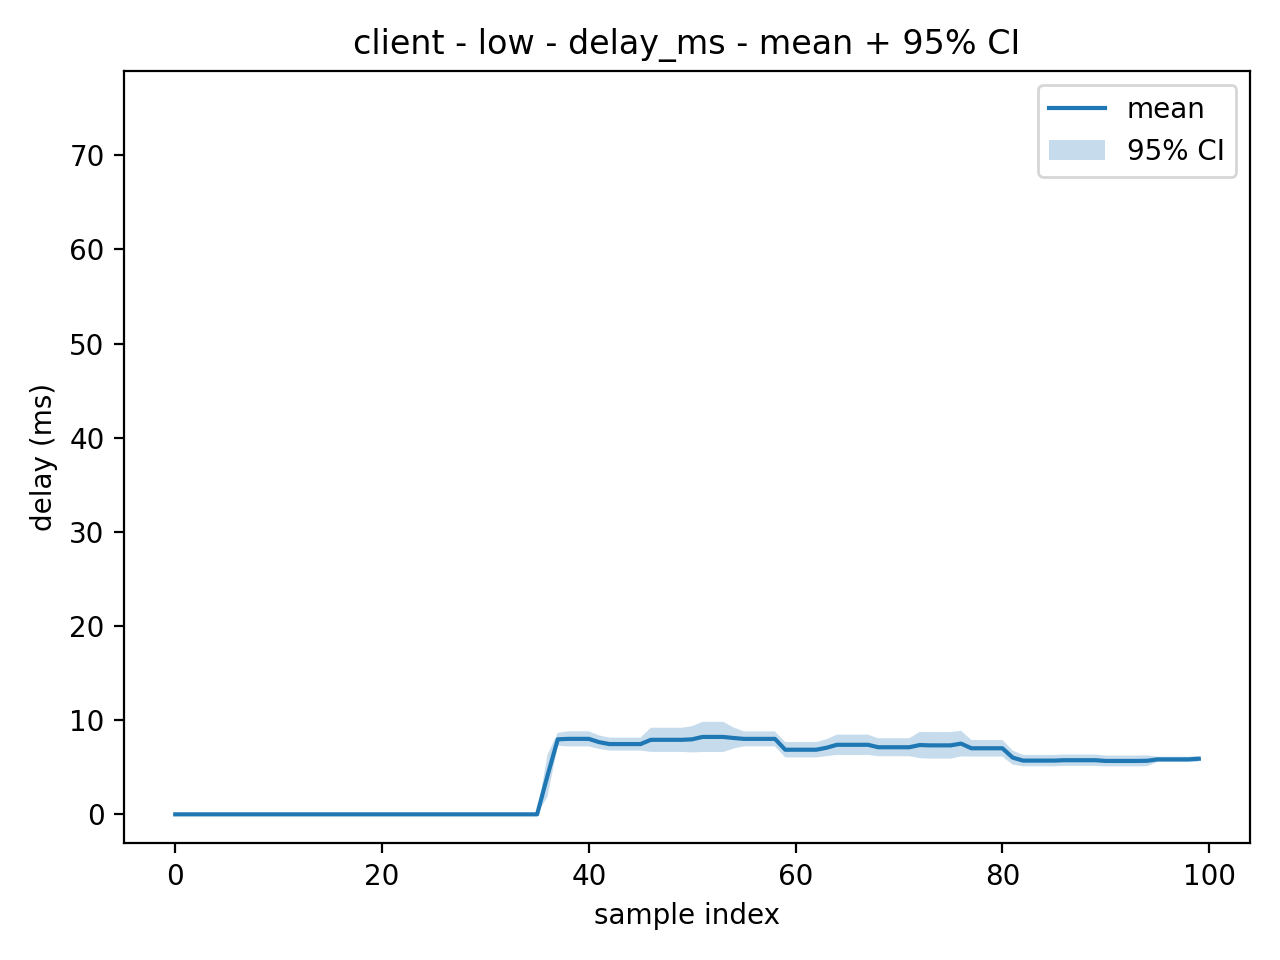
\includegraphics[width=\linewidth]{
      pars_plots/ntpsec/_aggregated/client/low/delay_ms_mean_ci95.png
    }
    \caption{Scenario LOW}
  \end{subfigure}
  \hfill
  \begin{subfigure}
    {0.32\textwidth}
    \centering
    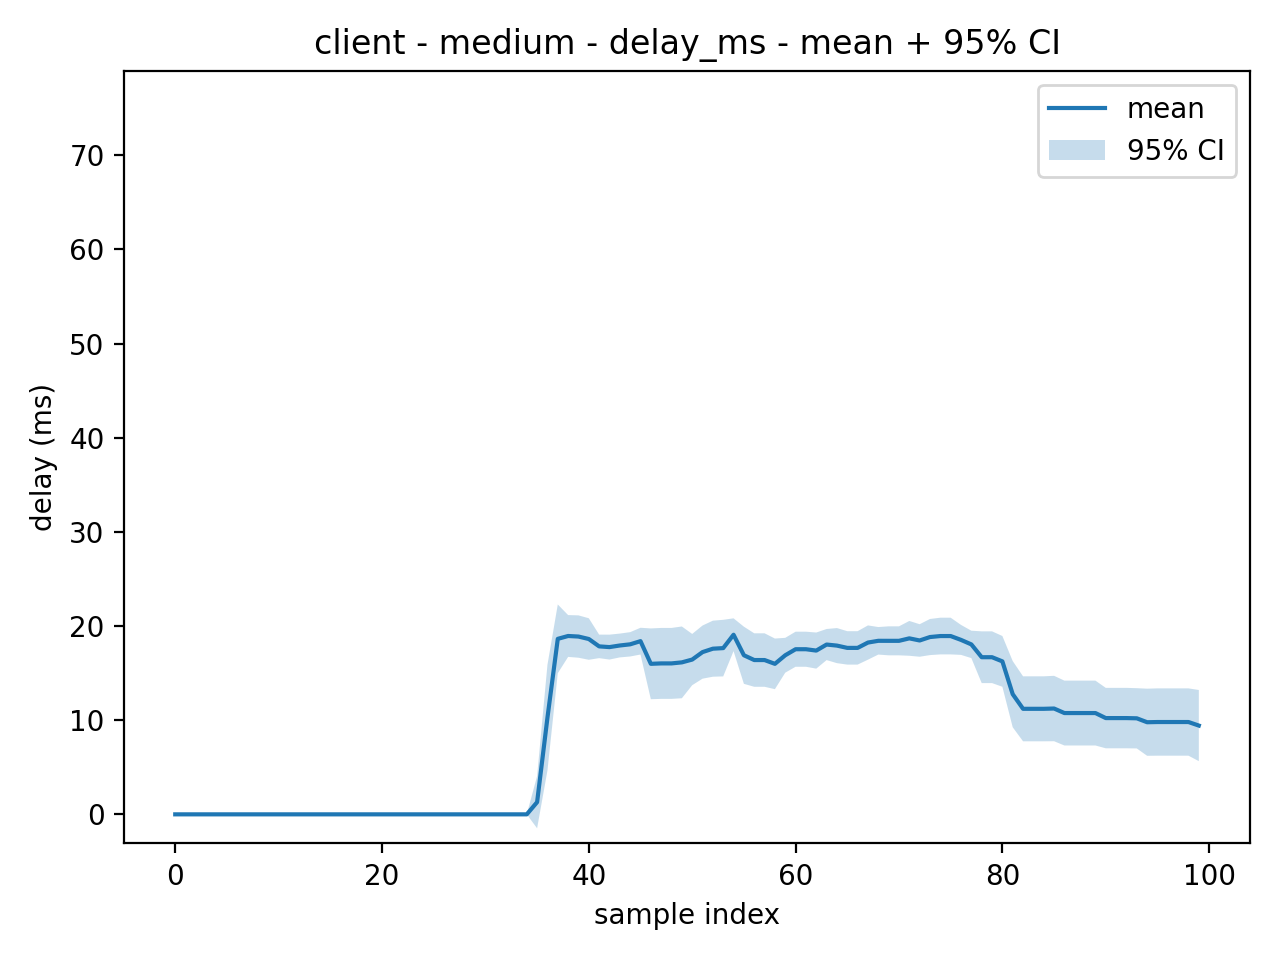
\includegraphics[width=\linewidth]{
      pars_plots/ntpsec/_aggregated/client/medium/delay_ms_mean_ci95.png
    }
    \caption{Scenario MEDIUM}
  \end{subfigure}
  \hfill
  \begin{subfigure}
    {0.32\textwidth}
    \centering
    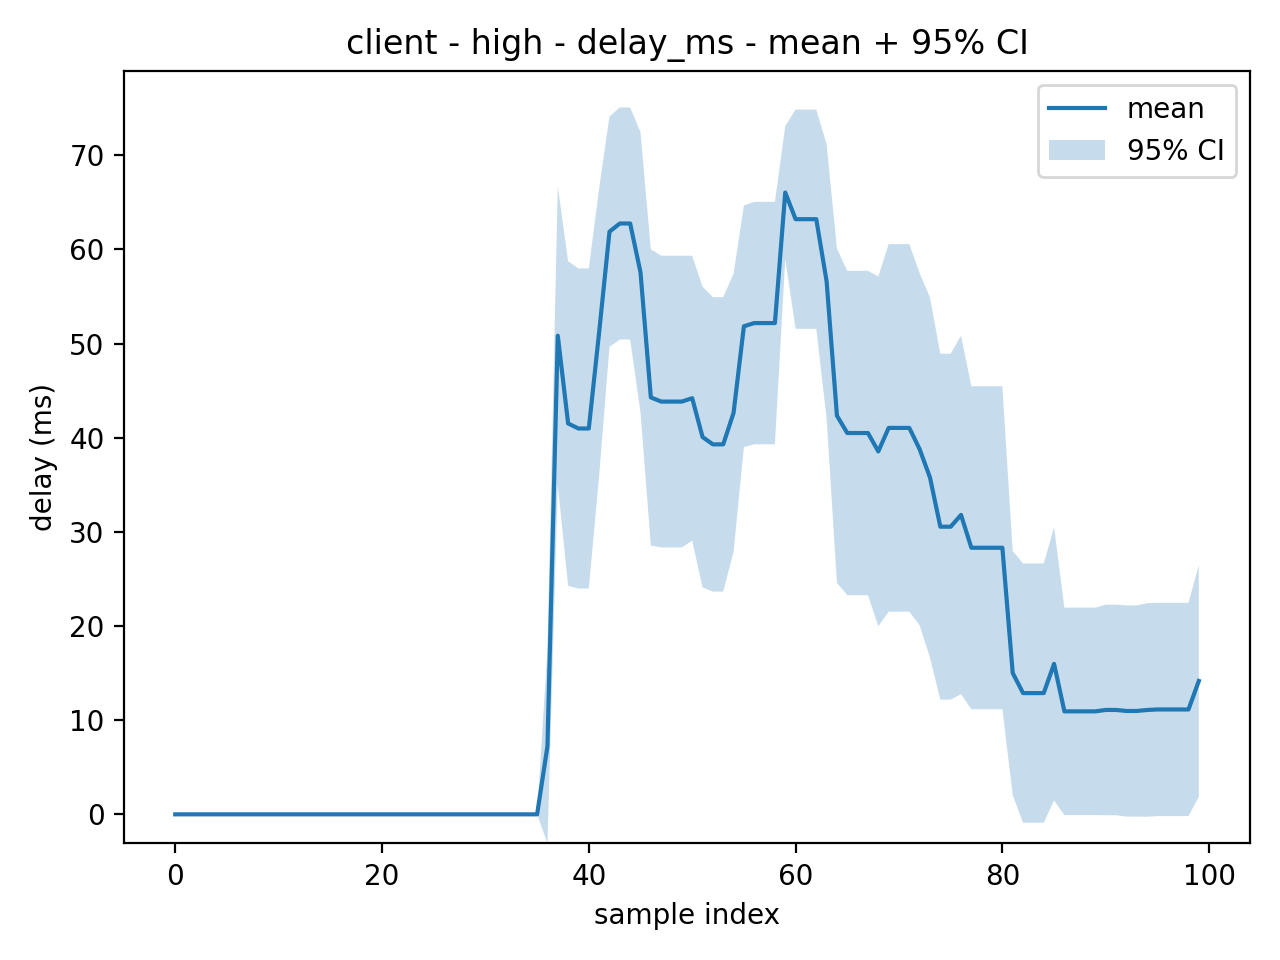
\includegraphics[width=\linewidth]{
      pars_plots/ntpsec/_aggregated/client/high/delay_ms_mean_ci95.png
    }
    \caption{Scenario HIGH}
  \end{subfigure}

  \caption{Media con intervallo di confidenza al 95\% - nodo: \texttt{clientntp}}
  \label{fig:scenario_comparison}
\end{figure}
\begin{figure}[H]
  \centering

  \begin{subfigure}
    {0.32\textwidth}
    \centering
    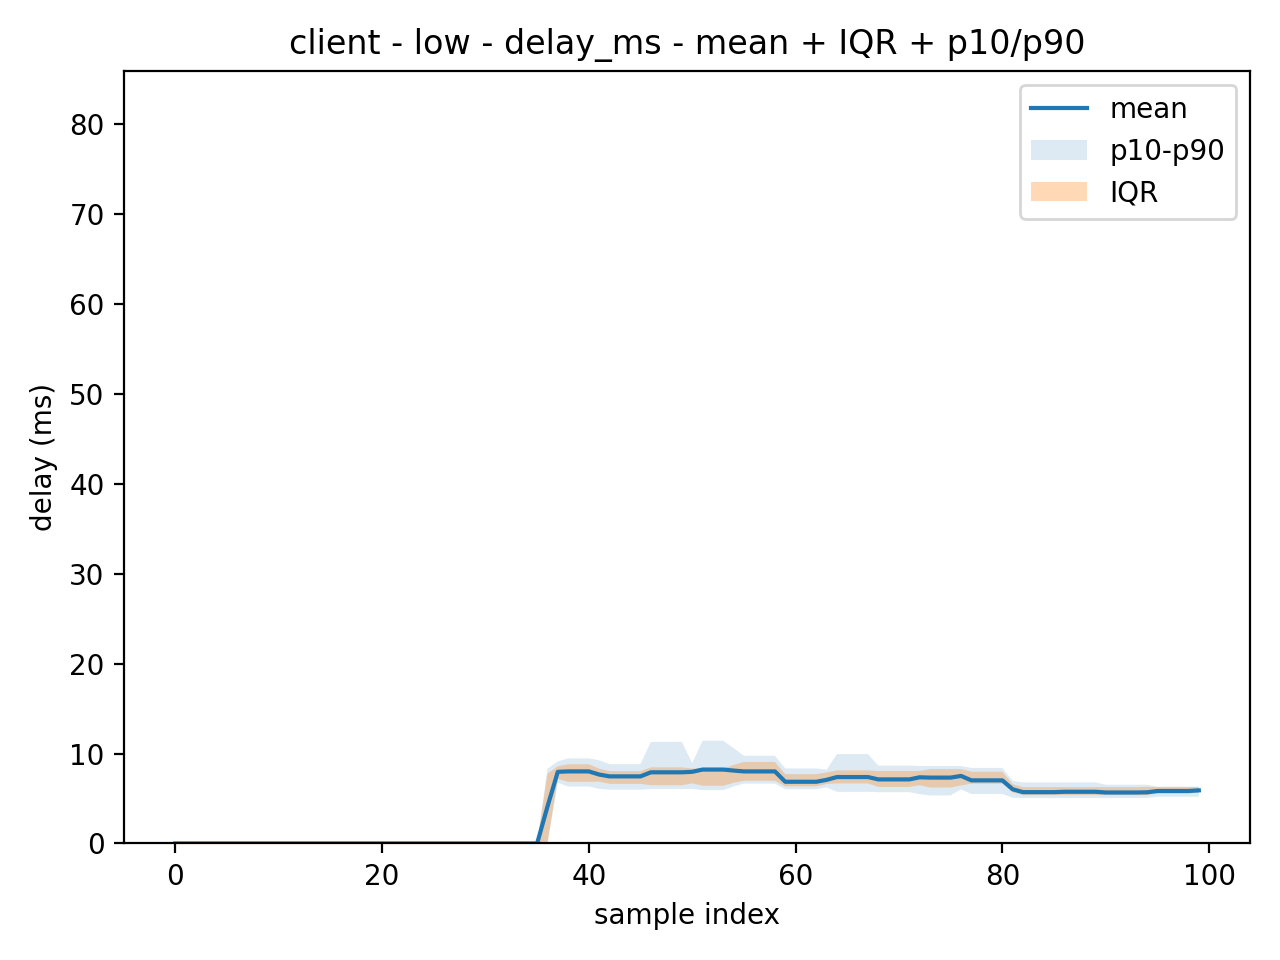
\includegraphics[width=\linewidth]{
      pars_plots/ntpsec/_aggregated/client/low/delay_ms_mean_iqr_p10_p90.png
    }
    \caption{Scenario LOW}
  \end{subfigure}
  \hfill
  \begin{subfigure}
    {0.32\textwidth}
    \centering
    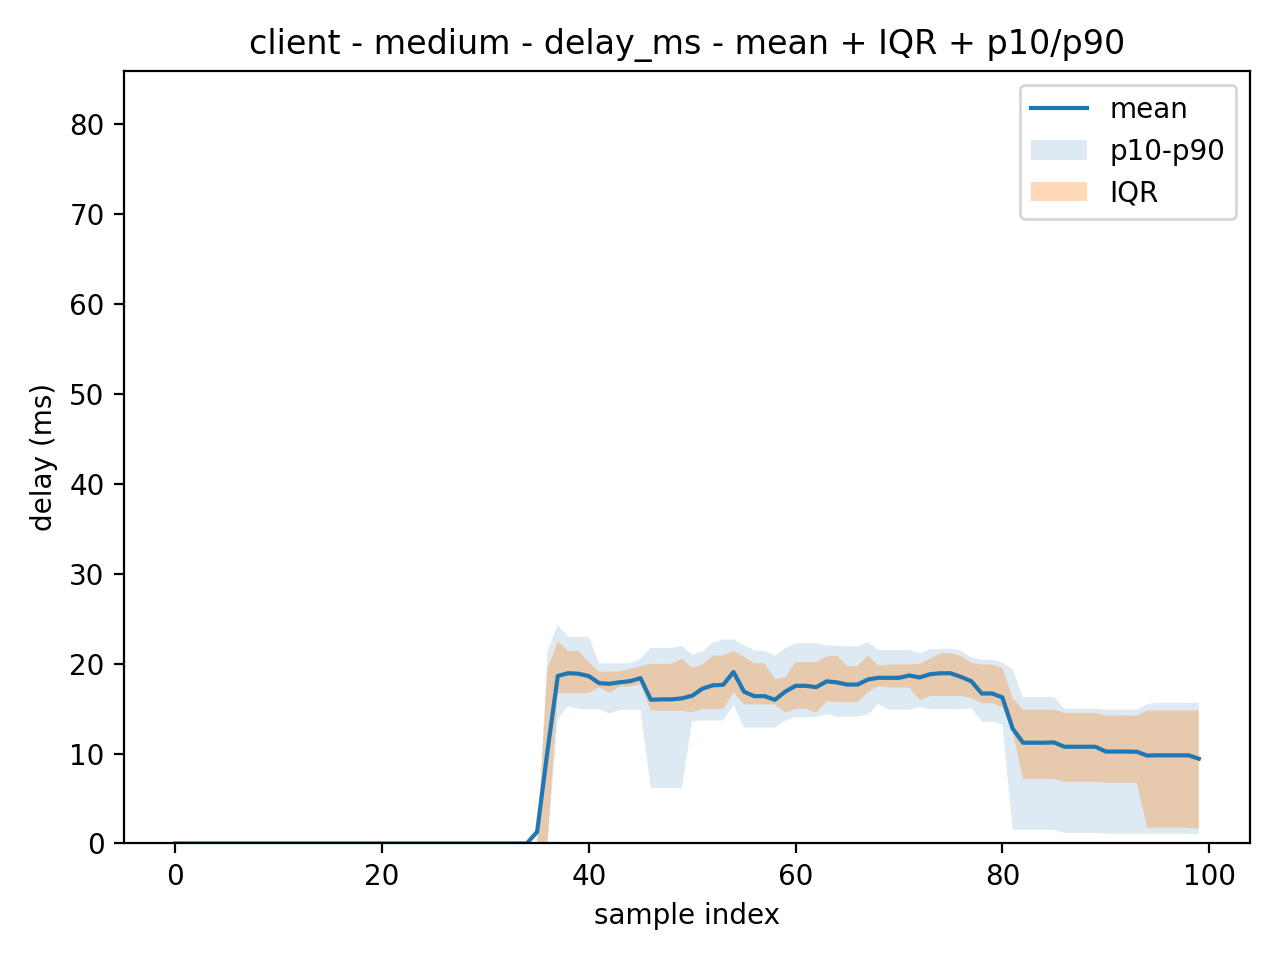
\includegraphics[width=\linewidth]{
      pars_plots/ntpsec/_aggregated/client/medium/delay_ms_mean_iqr_p10_p90.png
    }
    \caption{Scenario MEDIUM}
  \end{subfigure}
  \hfill
  \begin{subfigure}
    {0.32\textwidth}
    \centering
    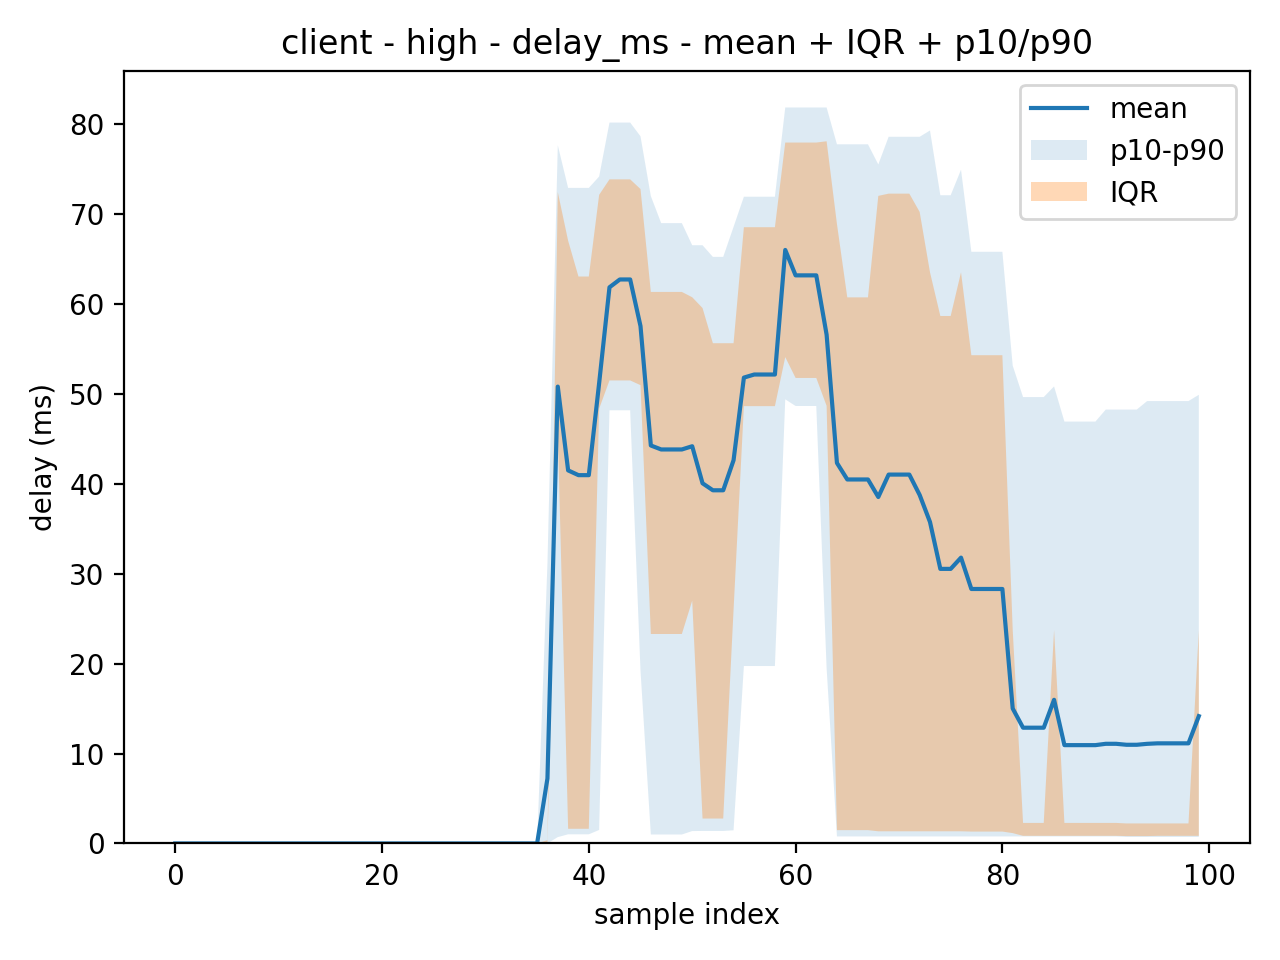
\includegraphics[width=\linewidth]{
      pars_plots/ntpsec/_aggregated/client/high/delay_ms_mean_iqr_p10_p90.png
    }
    \caption{Scenario HIGH}
  \end{subfigure}

  \caption{Media con banda inter-quartile e banda p10-p90 - nodo: \texttt{clientntp}}
  \label{fig:scenario_comparison}
\end{figure}

L'analisi del delay misurato sul nodo \texttt{clientntp} per il demone \texttt{NTPsec}
mette in evidenza una dipendenza dagli impairment di rete introdotte nei tre
scenari.

Nello scenario \texttt{low}, il delay assume valori contenuti e presenta un
andamento sostanzialmente regolare. La curva media si colloca stabilmente in una fascia
di circa 6–8 ms, con oscillazioni sufficientemente moderate con delle bande di
dispersione relativamente strette. Il delay medio è circa 7.00 ms, con una
mediana 6.82 ms e un intervallo inter-quartile uguale ~1.95 ms. La media della
banda inter-quartile di circa 1.43 ms, invece la larghezza media della banda p10–p90
è di circa 2.85 ms.

Nel caso \texttt{medium}, il delay cresce e si posiziona in una fascia superiore rispetto
al caso precedente. La curva media è nell'intervallo (16-19) ms per una parte
consistente dell'osservazione, per poi diminuire in fase finale verso valori ~10
ms. Il delay medio è ~15.5 ms, con mediana 16.5 ms e un intervallo inter-quartile di
~5.18 ms. L'IQR lungo la curva è ~5.62 ms e la p10–p90 ~10.0 ms.
Complessivamente l'andamento rimane leggibile e non ha instabilità estrema, evidenziando
comunque un peggioramento generale.

Nello scenario \texttt{high} si ha un comportamento con più degrado e meno
regolare. Post peer-selection, la curva media si posiziona in fase iniziale su
valori molto elevati, spesso compresi tra ~(40-65) ms, con oscillazioni ampie e una
forte eterogeneità tra run, evidenziato dall'ampliamento delle bande di
dispersione. Il livello medio è verso valori ~(10–15) ms. Il delay medio è pari a ~35.0
ms, con mediana 46.7 ms e l'intervallo inter-quartile molto ampio, pari a ~59.9 ms.
Le statistiche della curva aggregata confermano il trend, infatti si ha una
larghezza media della banda IQR è ~31.0 ms e quella p10–p90 ~59.4 ms.

Nel confronto tra scenari si evidenzia una progressione complessivamente coerente
con l'aumento della severità degli impairment di rete. Da \texttt{low} a \texttt{medium},
il delay del client cresce e contestualmente anche la sua dispersione,
mantenendo una dinamica ancora sufficientemente controllata. Nello scenario \texttt{high}
si evidenzia una maggiore discontinuità. Il livello medio è spostato su valori più
alti e lo stesso comportamento vale per la variabilità. Qualitativamente, la metrica
del delay risulta quindi efficace nel differenziare i tre scenari e nel mostrare come
l'incremento del degrado di rete si traduca in un peggioramento sia del livello della
misura sia della sua regolarità temporale.

\subsubsection{Analisi metrica: \texttt{jitter}}
\begin{figure}[H]
  \centering

  \begin{subfigure}
    {0.32\textwidth}
    \centering
    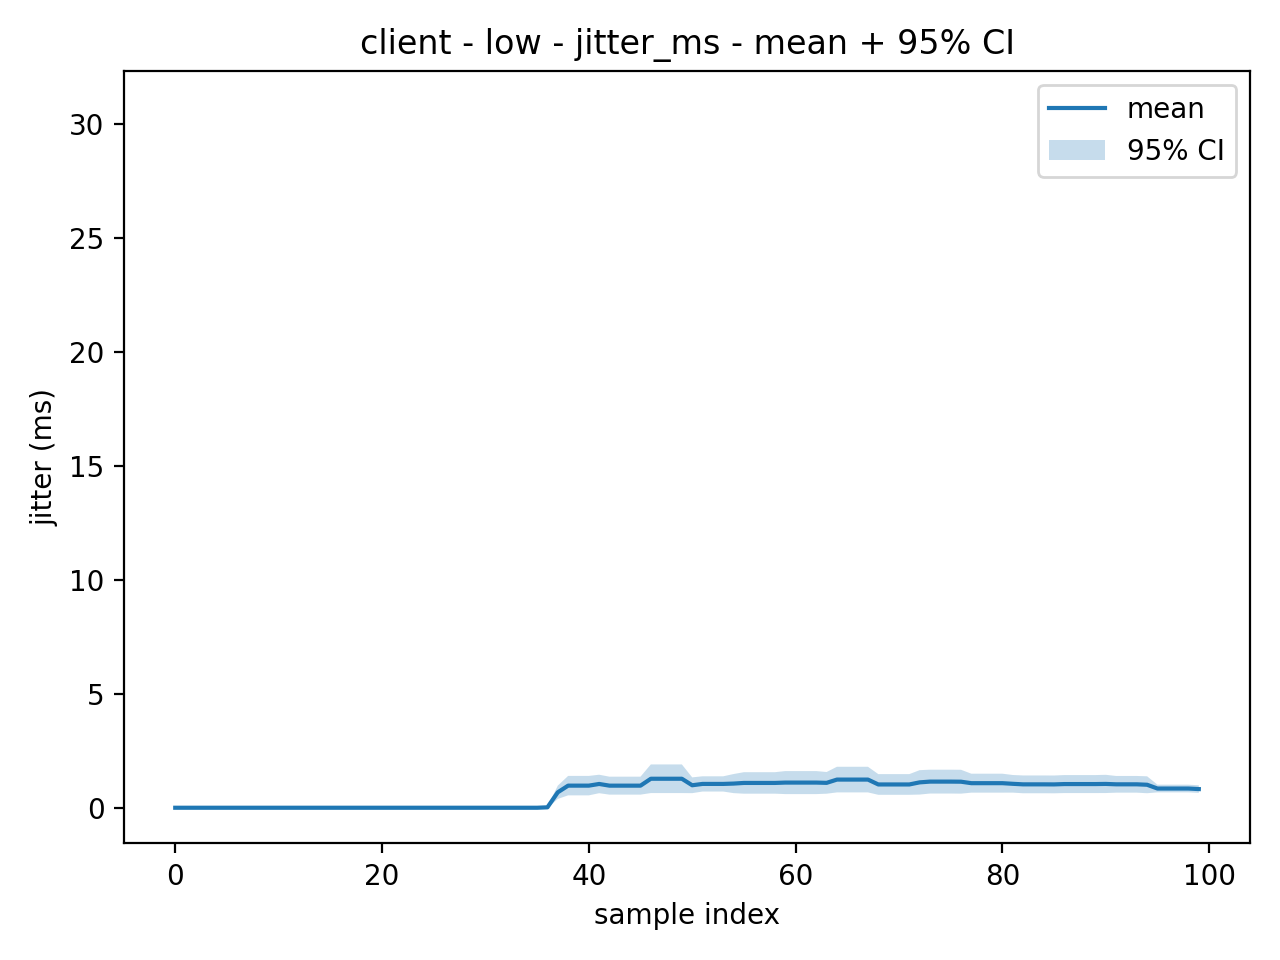
\includegraphics[width=\linewidth]{
      pars_plots/ntpsec/_aggregated/client/low/jitter_ms_mean_ci95.png
    }
    \caption{Scenario LOW}
  \end{subfigure}
  \hfill
  \begin{subfigure}
    {0.32\textwidth}
    \centering
    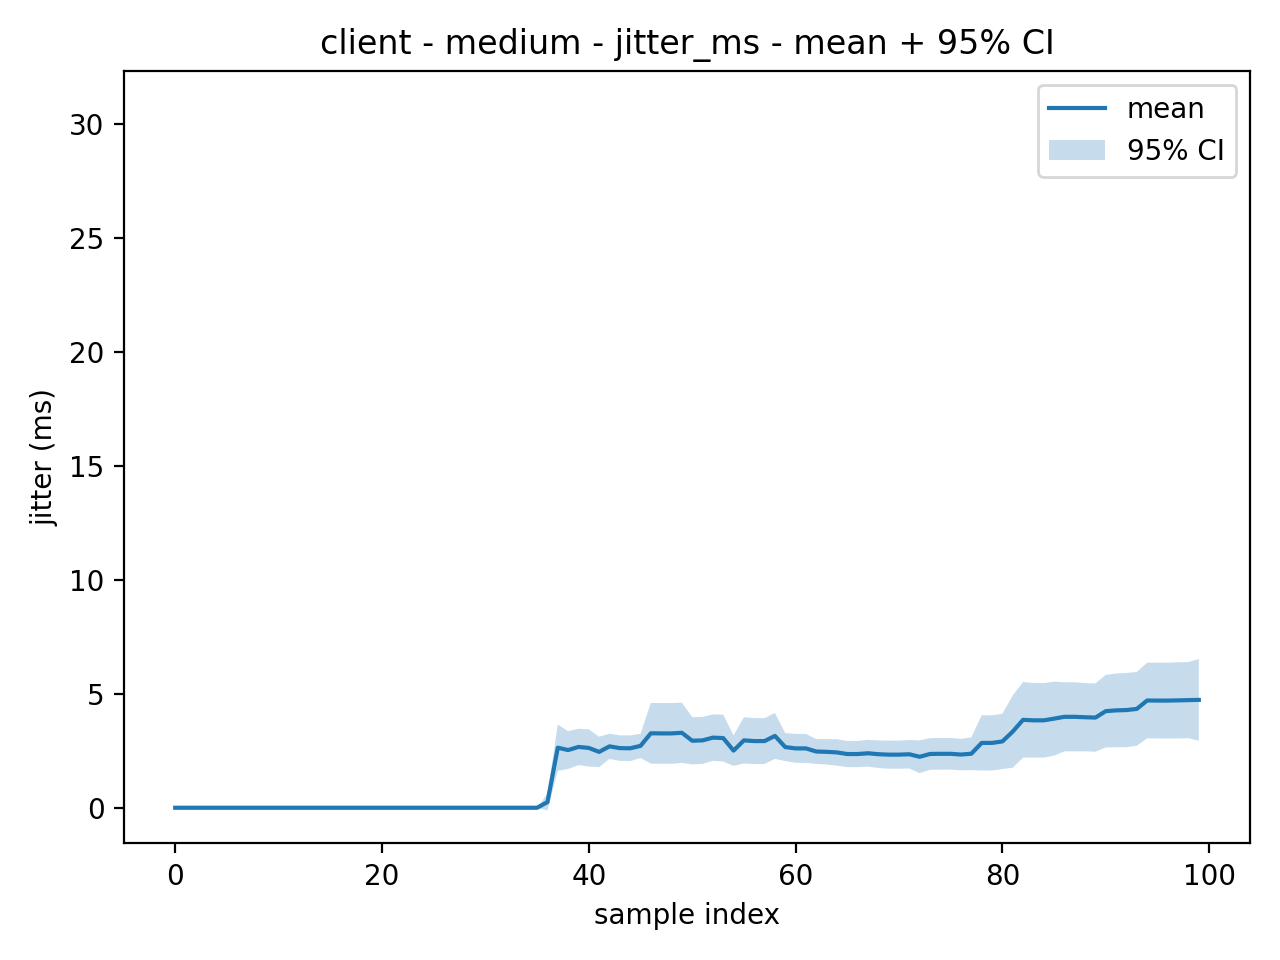
\includegraphics[width=\linewidth]{
      pars_plots/ntpsec/_aggregated/client/medium/jitter_ms_mean_ci95.png
    }
    \caption{Scenario MEDIUM}
  \end{subfigure}
  \hfill
  \begin{subfigure}
    {0.32\textwidth}
    \centering
    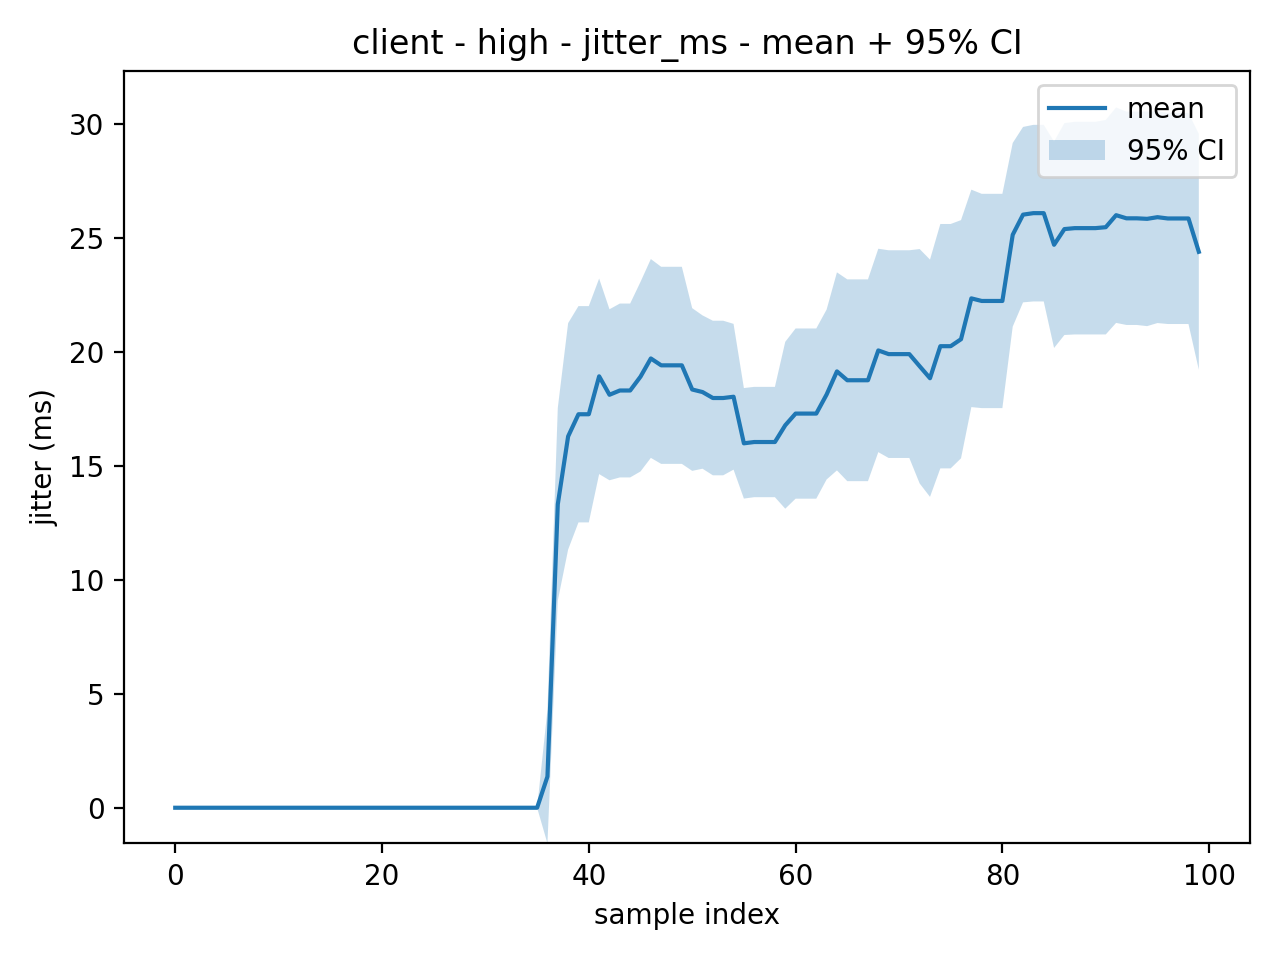
\includegraphics[width=\linewidth]{
      pars_plots/ntpsec/_aggregated/client/high/jitter_ms_mean_ci95.png
    }
    \caption{Scenario HIGH}
  \end{subfigure}

  \caption{Media con intervallo di confidenza al 95\% - nodo: \texttt{clientntp}}
  \label{fig:scenario_comparison}
\end{figure}
\begin{figure}[H]
  \centering

  \begin{subfigure}
    {0.32\textwidth}
    \centering
    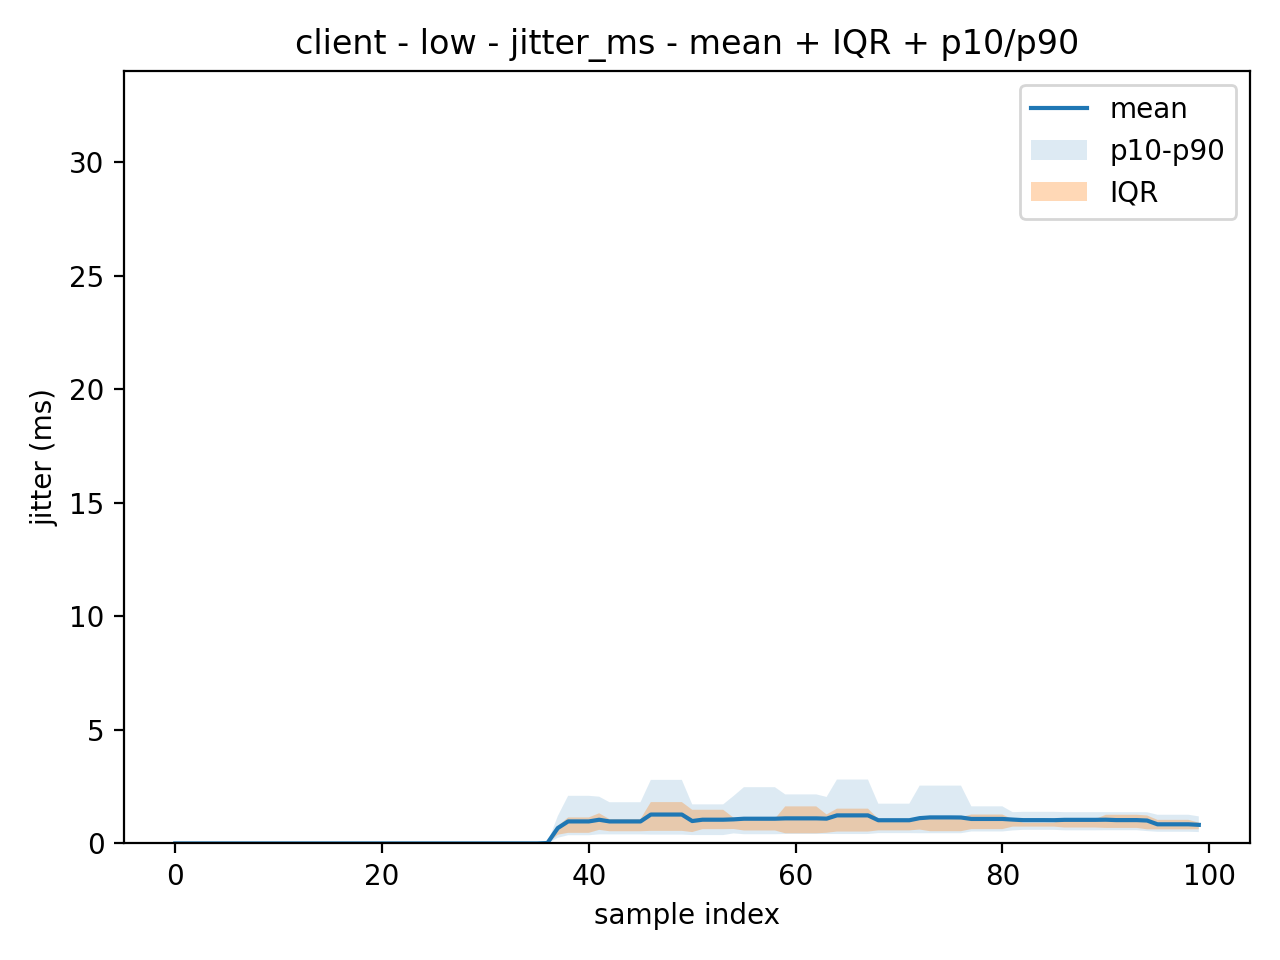
\includegraphics[width=\linewidth]{
      pars_plots/ntpsec/_aggregated/client/low/jitter_ms_mean_iqr_p10_p90.png
    }
    \caption{Scenario LOW}
  \end{subfigure}
  \hfill
  \begin{subfigure}
    {0.32\textwidth}
    \centering
    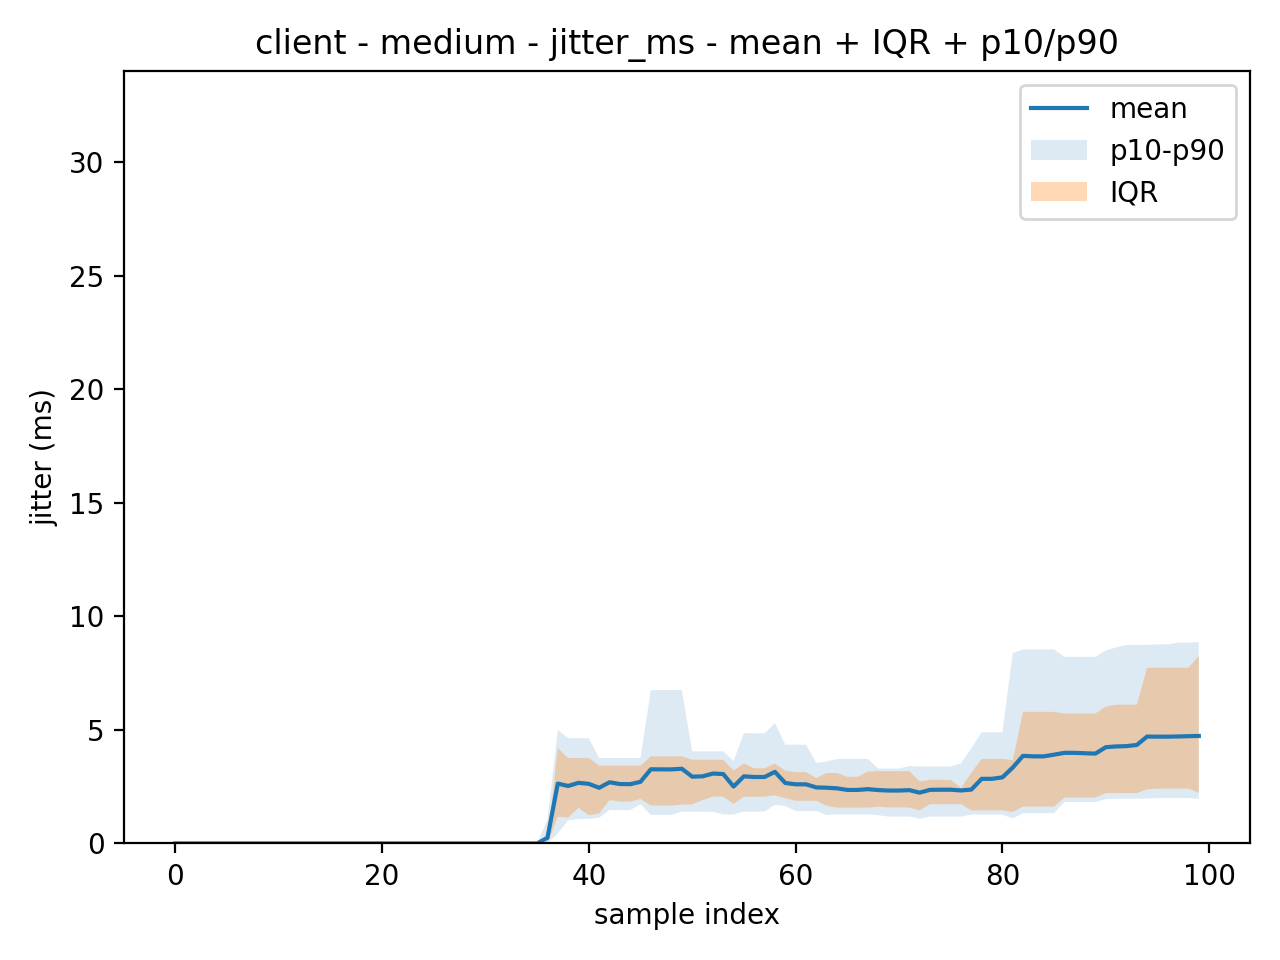
\includegraphics[width=\linewidth]{
      pars_plots/ntpsec/_aggregated/client/medium/jitter_ms_mean_iqr_p10_p90.png
    }
    \caption{Scenario MEDIUM}
  \end{subfigure}
  \hfill
  \begin{subfigure}
    {0.32\textwidth}
    \centering
    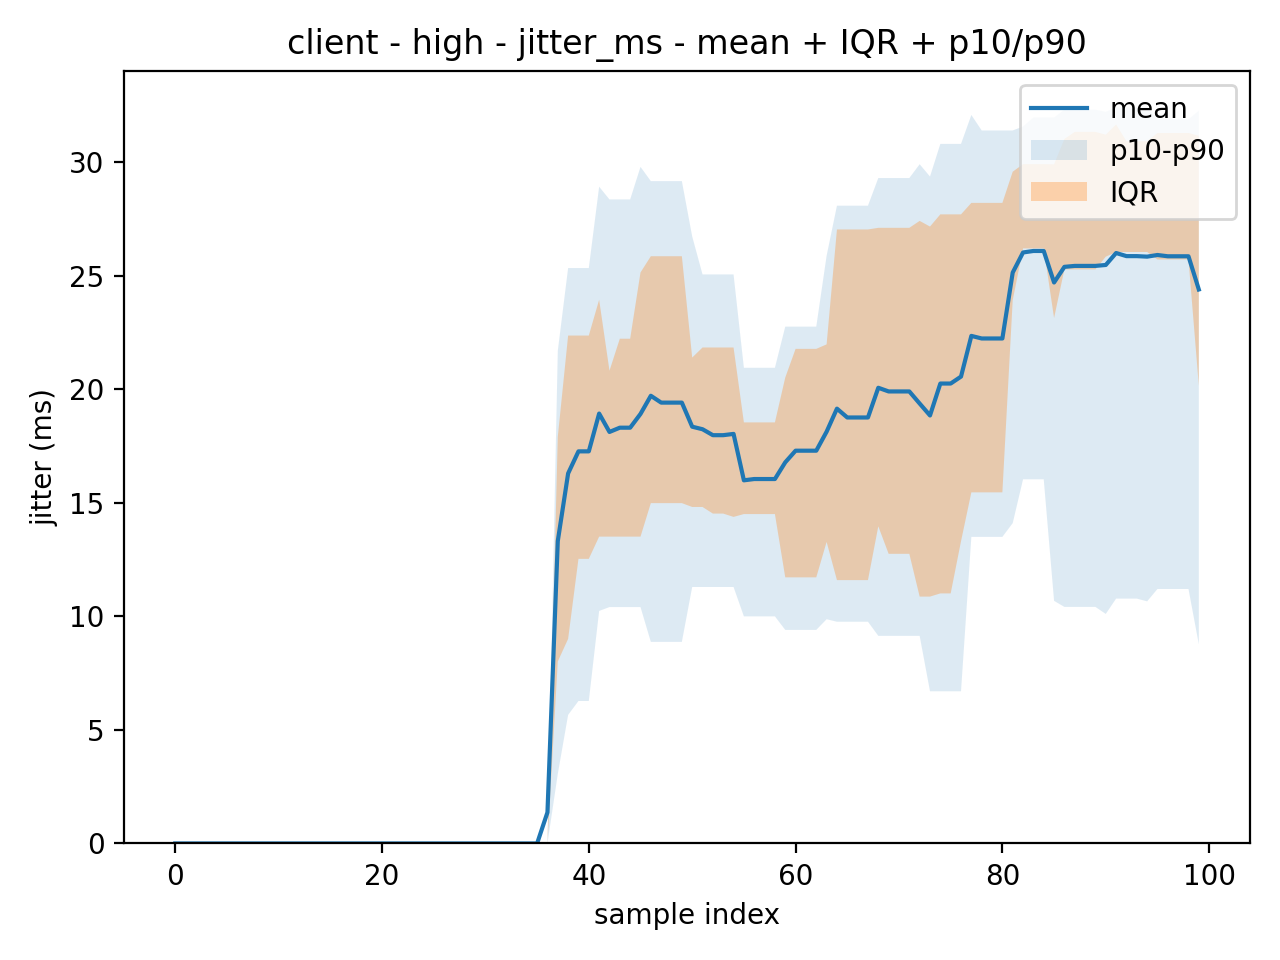
\includegraphics[width=\linewidth]{
      pars_plots/ntpsec/_aggregated/client/high/jitter_ms_mean_iqr_p10_p90.png
    }
    \caption{Scenario HIGH}
  \end{subfigure}

  \caption{Media con banda inter-quartile e banda p10-p90 - nodo: \texttt{clientntp}}
  \label{fig:scenario_comparison}
\end{figure}

L'analisi del jitter mostra un incremento di degrado attraverso un progressivo
aumento del livello medio e della variabilità.

Nello scenario \texttt{low} il valore medio risulta ~1.05 ms, con una dispersione
moderata. La banda inter-quartile media della curva aggregata è pari a ~0.65 ms,
invece la banda p10--p90 si attesta intorno a ~1.46 ms. Il comportamento osservato
è coerente con un degrado debole, evidenziando una condizione di rete stabile.

Nel caso \texttt{medium}, il jitter cresce in modo evidente e si posiziona su
una fascia sensibilmente superiore.Il valore medio è ~3.14 ms, all'incirca tre
volte il corrispondente valore osservato nello scenario \texttt{low}. Si ha un
aumento della dispersione, con banda inter-quartile media di ~2.40 ms e banda p10--p90
di ~4.18 ms.

Nello scenario \texttt{high} si manifesta un degradato più marcato. Il jitter
assume valori elevati lungo l'intera serie aggregata, con una media all'incirca di
20.9 ms. Sia ha un incremento rispetto agli scenari precedenti, in particolare rispetto
allo scenario \texttt{low}, con un divario di un ordine di grandezza. La
dispersione misurata aumenta con banda inter-quartile media ~9.38 ms e banda p10--p90
di circa 18.3 ms. Nel grafico si evidenzia una forte oscillazione, ampia e
persiste.

Vi è un generale aumento coerente con il degrado di rete, evidenziando un impatto
maggiore da gli scenari \texttt{low-medium} allo scenario \texttt{high} caratterizzato
da valori medi elevati e da una dispersione significativamente maggiore.

\subsubsection{Analisi metrica: \texttt{offset}}
\begin{figure}[H]
  \centering

  \begin{subfigure}
    {0.32\textwidth}
    \centering
    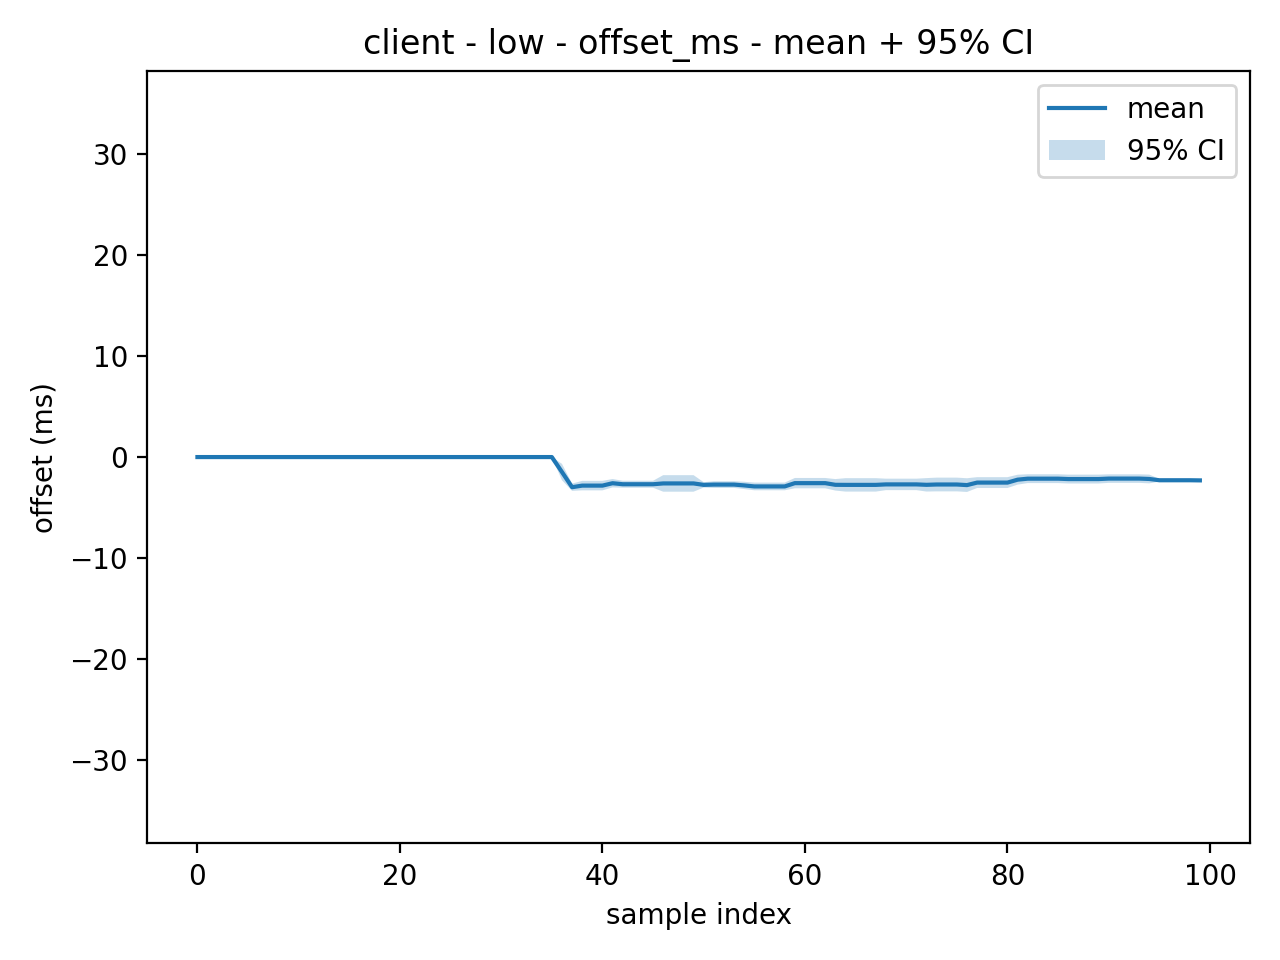
\includegraphics[width=\linewidth]{
      pars_plots/ntpsec/_aggregated/client/low/offset_ms_mean_ci95.png
    }
    \caption{Scenario LOW}
  \end{subfigure}
  \hfill
  \begin{subfigure}
    {0.32\textwidth}
    \centering
    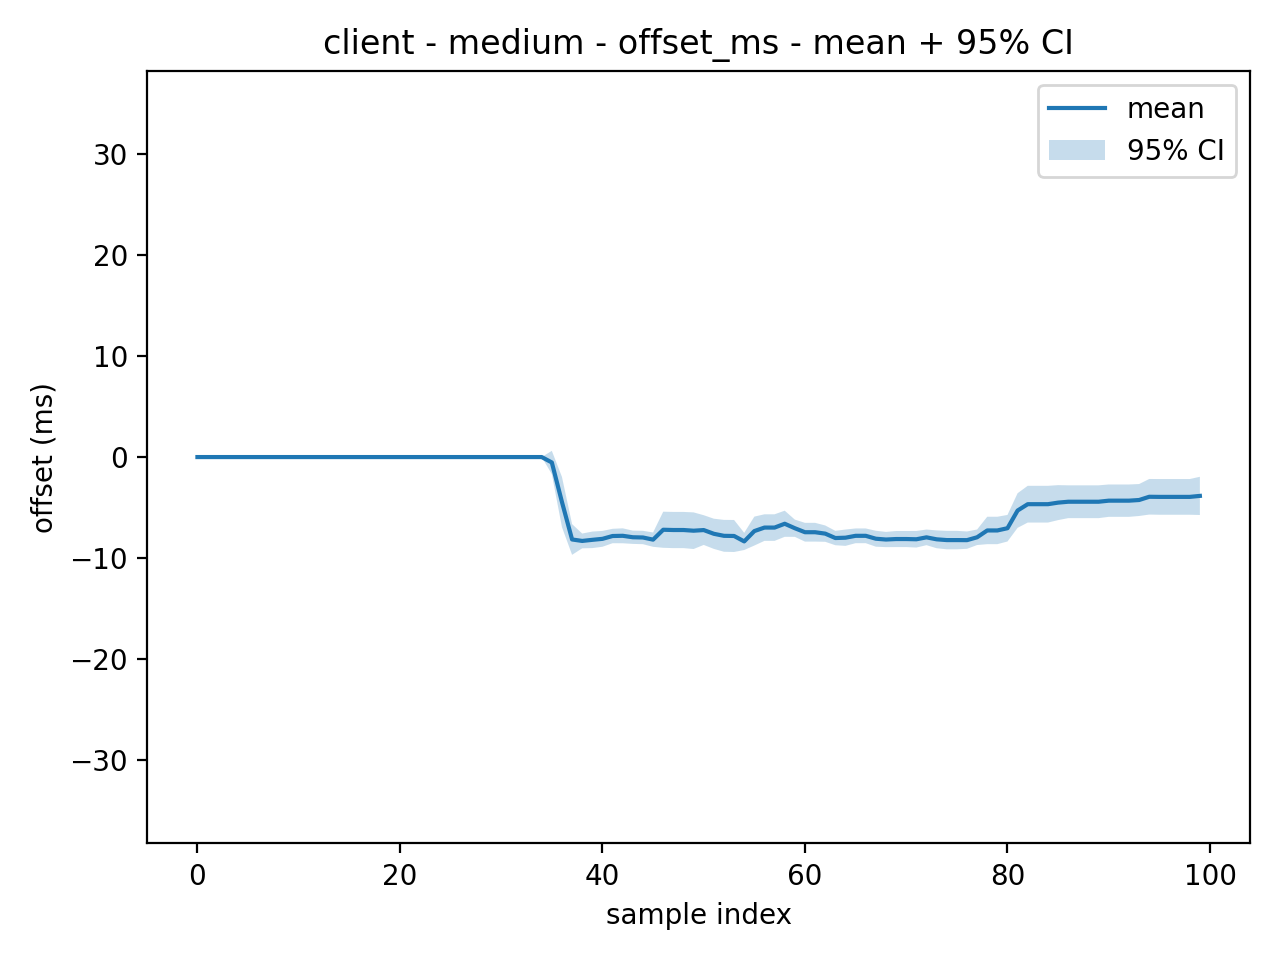
\includegraphics[width=\linewidth]{
      pars_plots/ntpsec/_aggregated/client/medium/offset_ms_mean_ci95.png
    }
    \caption{Scenario MEDIUM}
  \end{subfigure}
  \hfill
  \begin{subfigure}
    {0.32\textwidth}
    \centering
    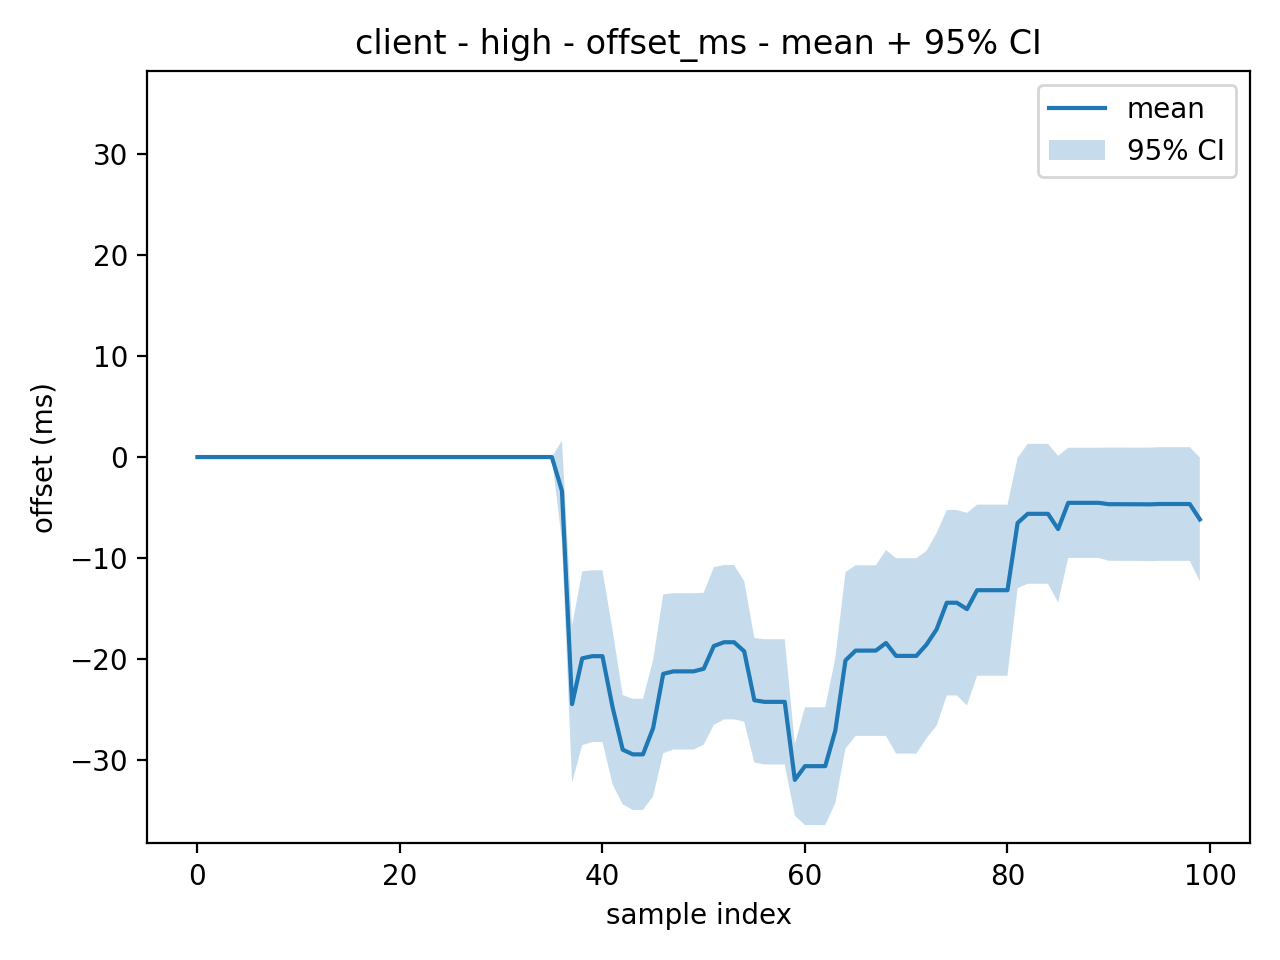
\includegraphics[width=\linewidth]{
      pars_plots/ntpsec/_aggregated/client/high/offset_ms_mean_ci95.png
    }
    \caption{Scenario HIGH}
  \end{subfigure}

  \caption{Media con intervallo di confidenza al 95\% - nodo: \texttt{clientntp}}
  \label{fig:scenario_comparison}
\end{figure}
\begin{figure}[H]
  \centering

  \begin{subfigure}
    {0.32\textwidth}
    \centering
    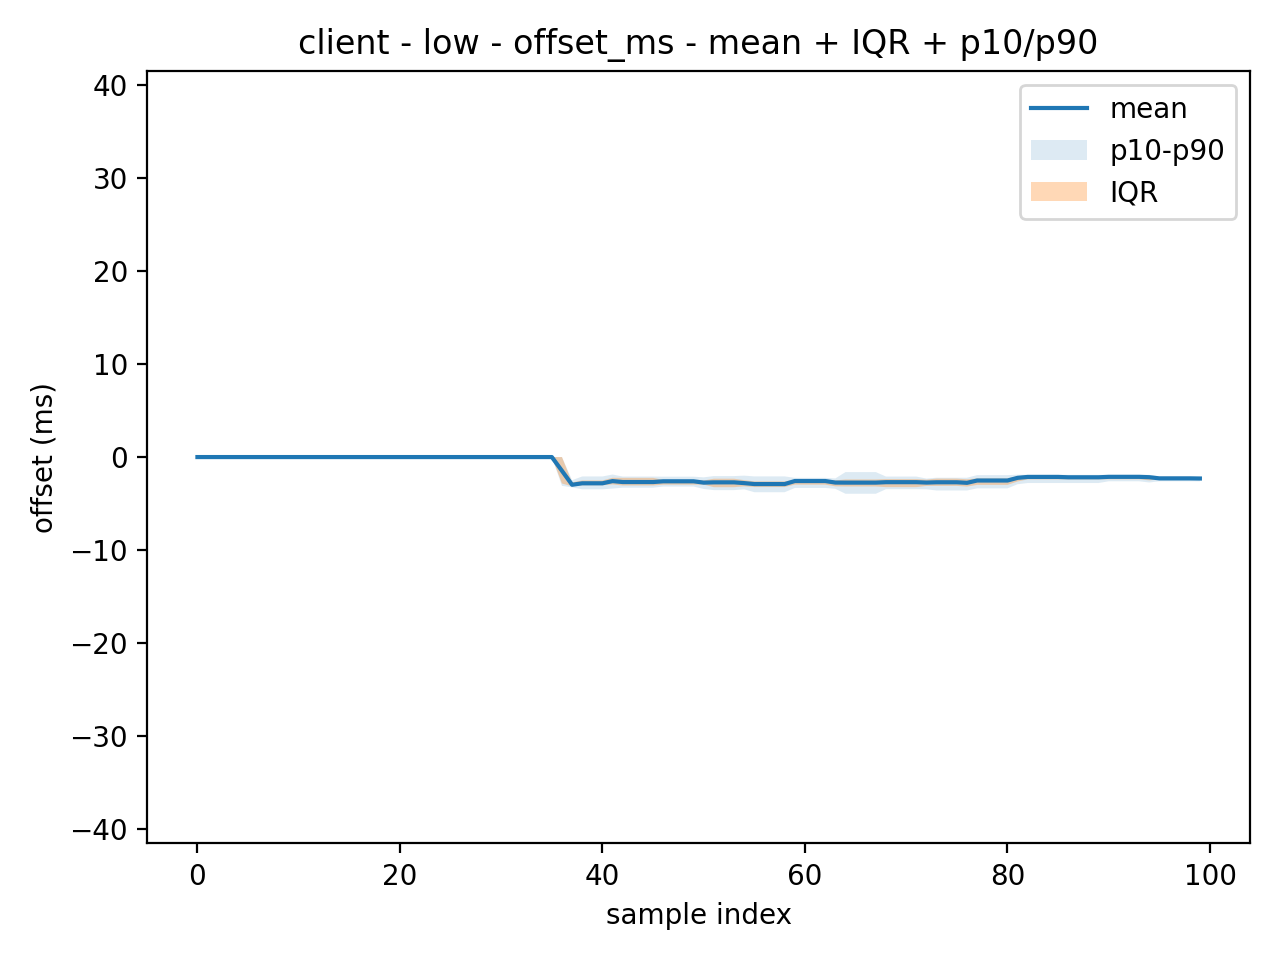
\includegraphics[width=\linewidth]{
      pars_plots/ntpsec/_aggregated/client/low/offset_ms_mean_iqr_p10_p90.png
    }
    \caption{Scenario LOW}
  \end{subfigure}
  \hfill
  \begin{subfigure}
    {0.32\textwidth}
    \centering
    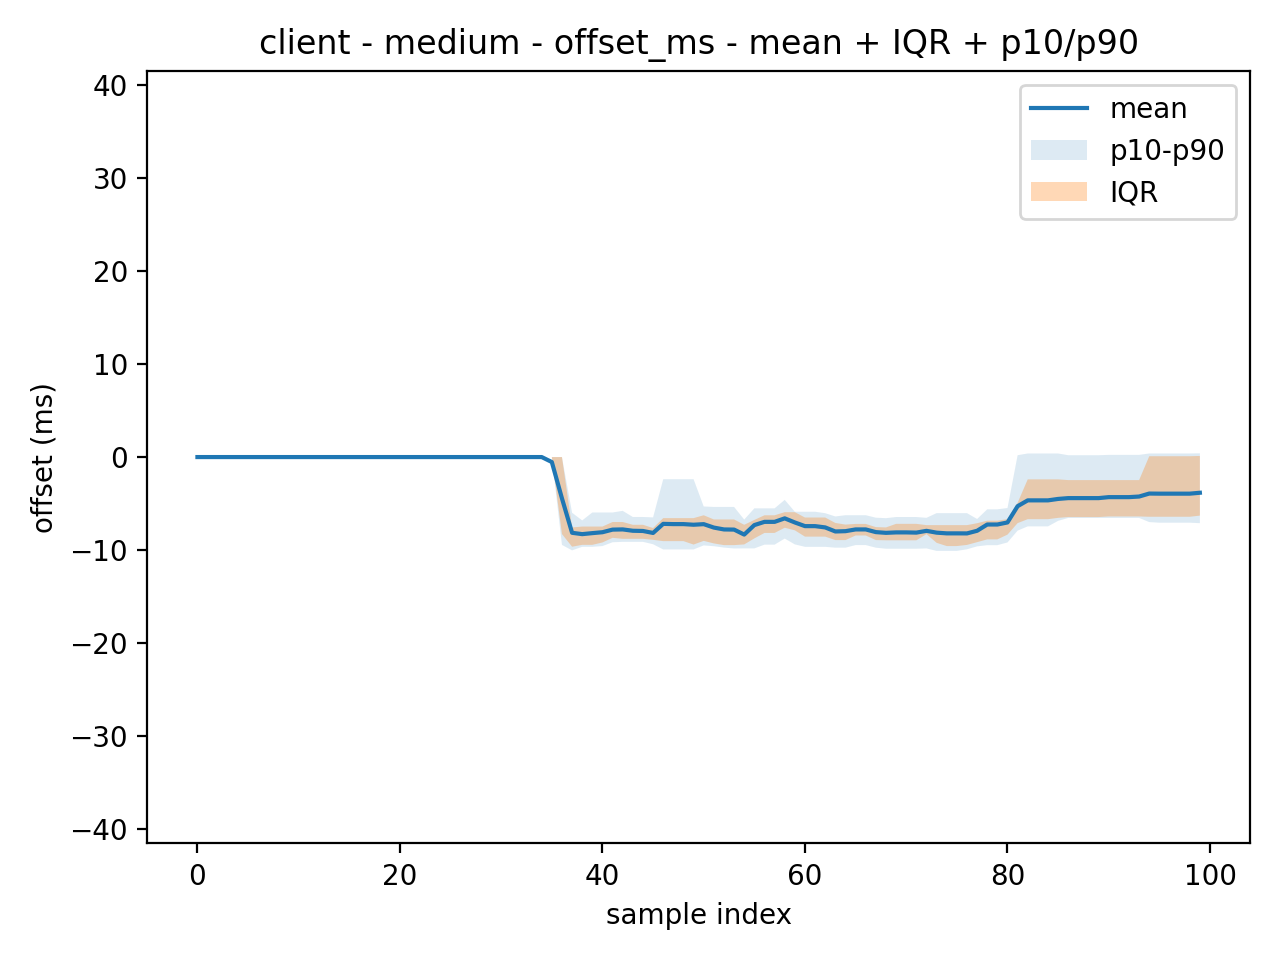
\includegraphics[width=\linewidth]{
      pars_plots/ntpsec/_aggregated/client/medium/offset_ms_mean_iqr_p10_p90.png
    }
    \caption{Scenario MEDIUM}
  \end{subfigure}
  \hfill
  \begin{subfigure}
    {0.32\textwidth}
    \centering
    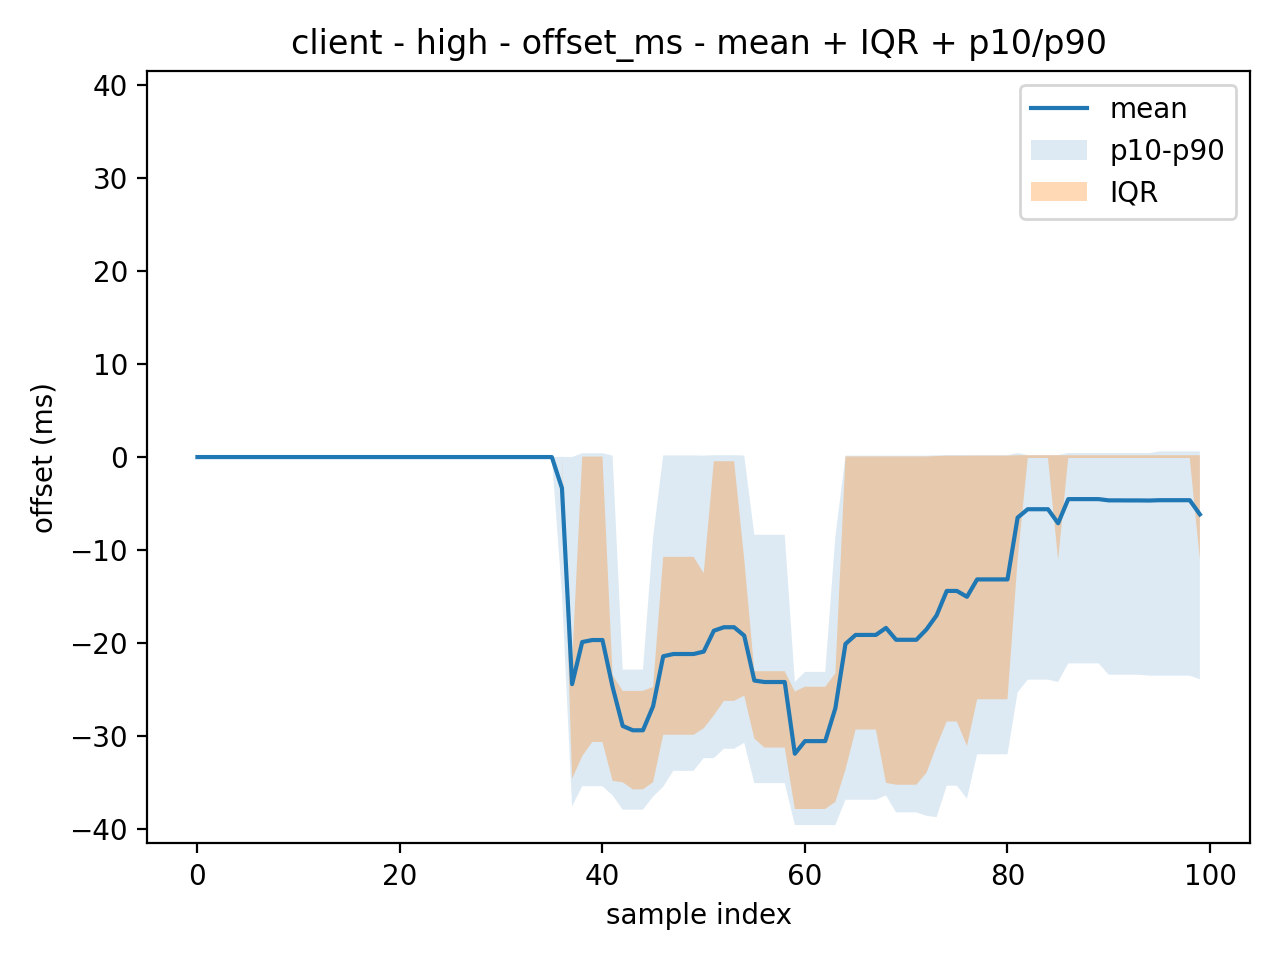
\includegraphics[width=\linewidth]{
      pars_plots/ntpsec/_aggregated/client/high/offset_ms_mean_iqr_p10_p90.png
    }
    \caption{Scenario HIGH}
  \end{subfigure}

  \caption{Media con banda inter-quartile e banda p10-p90 - nodo: \texttt{clientntp}}
  \label{fig:scenario_comparison}
\end{figure}

Nell'analisi dell'offset si evidenziano valori sistematicamente negativi.

Nello scenario \texttt{low}, l'offset si stabilizza su valori nell'intervallo ~$-
2.5$/$-3\,\mathrm{ms}$. La media è di ~$-2.55\,\mathrm{ms}$. La mediana è
pressoché identica, $-2 .55\,\mathrm{ms}$. La dispersione è moderata, ($\sigma \approx
0.91\,\mathrm{ms}$). La curva aggregata conferma il trend con un valore medio
centrale di $-2.55\,\mathrm{ms}$, invece l'ampiezza banda inter-quartile è di ~($\mathrm{IQR}
\approx 0.56\,\mathrm{ms}$) e la fascia $p10$--$p 90$ di circa ($\approx 1.21\,\mathrm{ms}$).Il
comportamento è stabile e uno scostamento limitato rispetto al riferimento.

Nel caso \texttt{medium} si ha un offset traslato su valori più marcati (negativi).
La misura è in un intervallo di $-7$/$-8\,\mathrm{ms}$, con un aumento nella
fase finale della serie. La media è ~$-6.70\,\mathrm{ms}$, con mediana pari a $-7
.08\,\mathrm{ms}$. La deviazione standard è di ~$2.81\,\mathrm{ms}$. La curva
aggregata rimane coerente con un valor medio centrale di $-6.69\,\mathrm{ms}$. C'è
una crescita anche della variabilità, mostrato dall'ampiezza media della banda
inter-quartile ($\approx 2.74\,\mathrm{ms}$) e della fascia $p10$--$p90$ ($\approx
4.97\,\mathrm{ms}$).

Lo scenario \texttt{high}, conferma il trend. La curva aggregata evidenzia una
prolungata permanenza dei valori in una fascia di circa $-20$ e
$-30\,\mathrm{ms}$ per poi avere valori che si stabiliscono nella parte finale
della run. La media pari a circa $-16.42\,\mathrm{ms}$, la mediana a
$-21.87\,\mathrm{ms}$ e la deviazione standard a circa $15.38\,\mathrm{ms}$
confermano quanto osservato. Vi è una dispersione superiore rispetto agli altri scenari.
L'ampiezza media della banda inter-quartile è di ~$15 .17\,\mathrm{ms}$, La
fascia $p10$--$p90$ di ~$29.44\, \mathrm{ms}$. Il minimo della curva media aggregata
scende inoltre fino a circa $-30.12\,\mathrm{ms}$.
Nella fase finale si osserva una presenza più marcata dagli outlier, con una curva media
esterna alla banda inter-quartile.

La misura dell'offset conferma un coerente e progressivo degrado al variare degli
impairment. Nello scenario \texttt{high} si ha un peggioramento marcato.

\subsection{\texttt{boundary}}
Nel caso del nodo \texttt{boundary} vi è necessario fare un considerazione
preliminare. A differenza di quanto osservato sul nodo \texttt{clientntp}, gli impairment
di rete introdotti mediante \texttt{tc/netem} non impattano direttamente sul
collegamento \texttt{upstream} tra il nodo \texttt{boundary} e il nodo di
riferimento ma solamente nel ramo \texttt{downstream} tra \texttt{boundary} e
\texttt{clientntp}. Di conseguenza le metriche osservate non dovrebbero, in linea
teorica, risentirne. La sezione seguente quindi, ha come scopo verificare se i
dati sono coerenti con il sistema.

L'analisi è quindi orientata principalmente a verificare la coerenza tra tale
aspettativa teorica e i dati effettivamente osservati.

È utile notare che nell'analisi il tempo di peer-selection differente rispetto a
quello osservato sul nodo \texttt{clientntp} è tenuto in considerazione.

\subsubsection{Analisi metriche: \texttt{delay, jitter, offset}}
\begin{figure}[H]
  \centering

  \begin{subfigure}
    {0.32\textwidth}
    \centering
    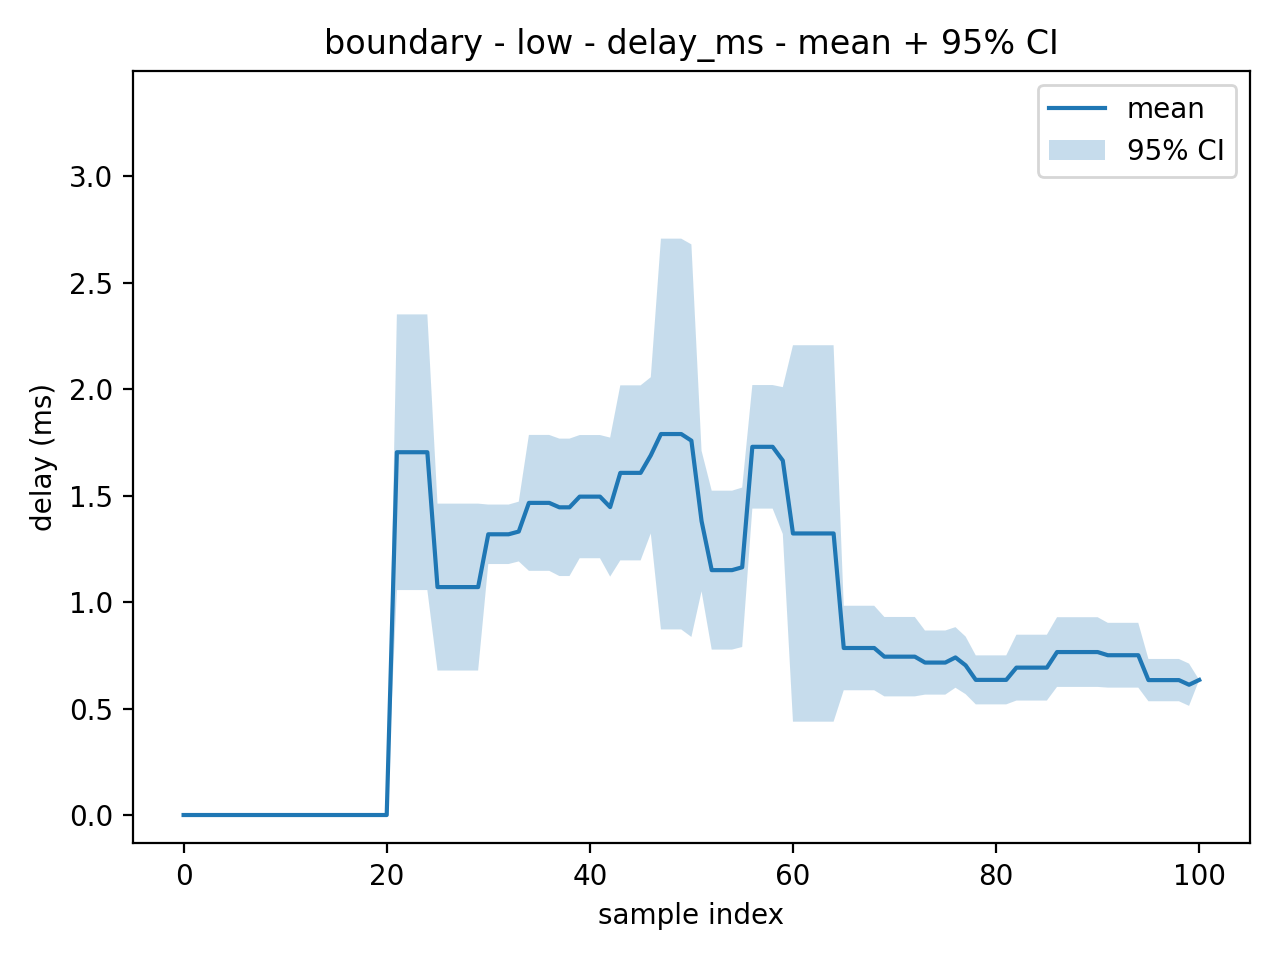
\includegraphics[width=\linewidth]{
      pars_plots/ntpsec/_aggregated/boundary/low/delay_ms_mean_ci95.png
    }
    \caption{Scenario LOW}
  \end{subfigure}
  \hfill
  \begin{subfigure}
    {0.32\textwidth}
    \centering
    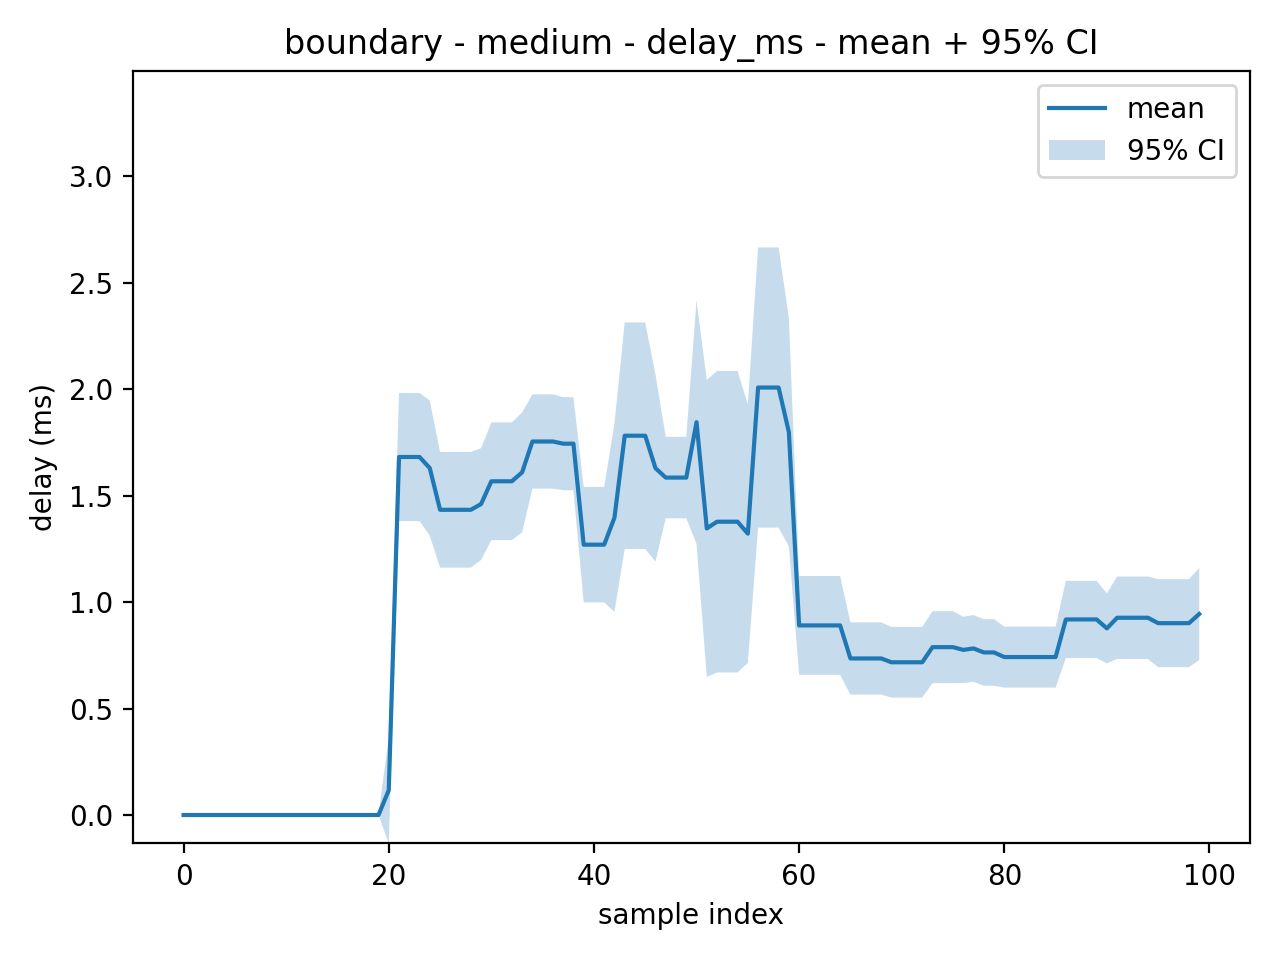
\includegraphics[width=\linewidth]{
      pars_plots/ntpsec/_aggregated/boundary/medium/delay_ms_mean_ci95.png
    }
    \caption{Scenario MEDIUM}
  \end{subfigure}
  \hfill
  \begin{subfigure}
    {0.32\textwidth}
    \centering
    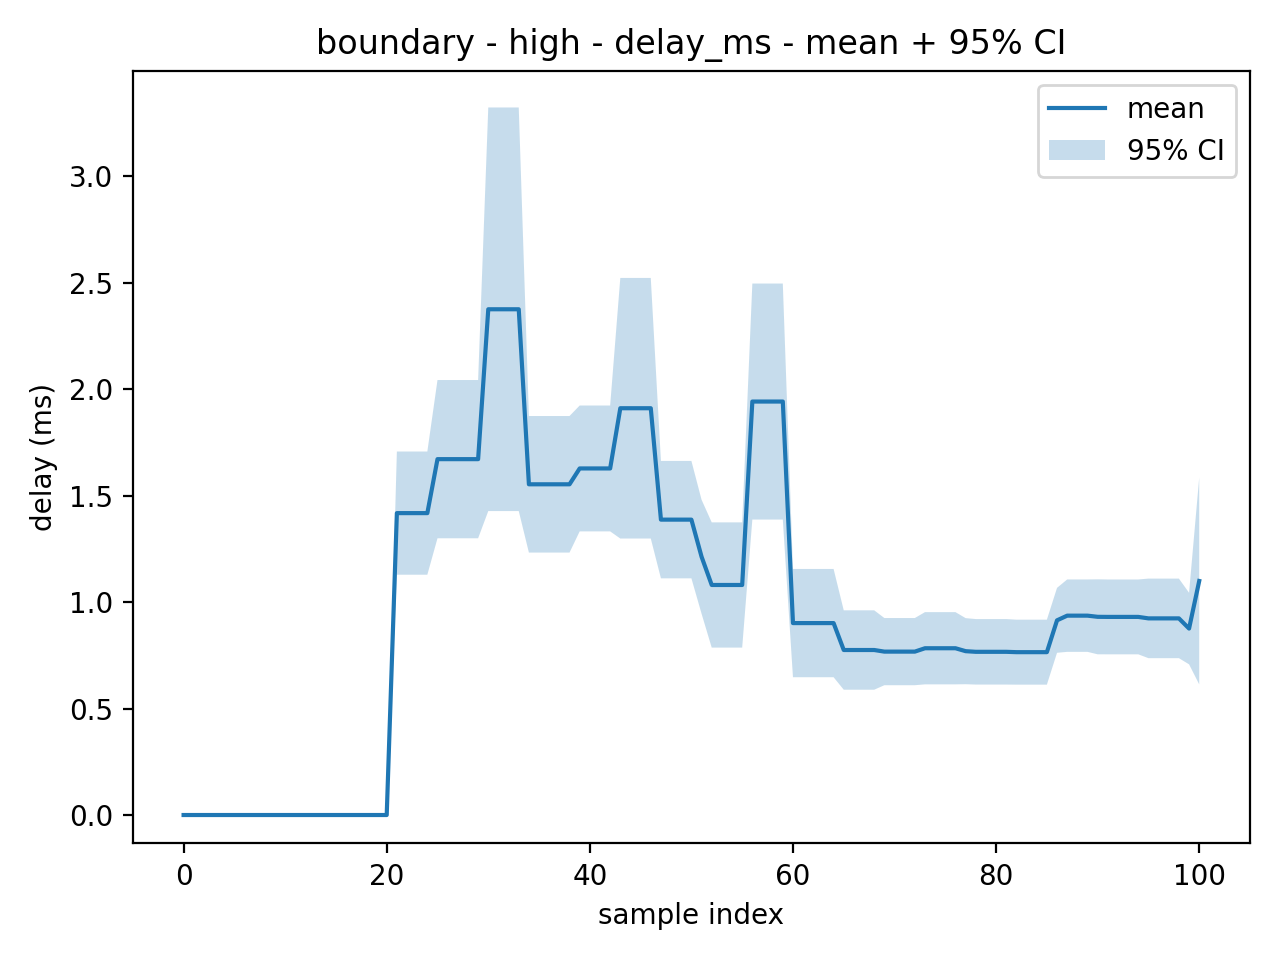
\includegraphics[width=\linewidth]{
      pars_plots/ntpsec/_aggregated/boundary/high/delay_ms_mean_ci95.png
    }
    \caption{Scenario HIGH}
  \end{subfigure}

  \caption{Media con intervallo di confidenza al 95\% - nodo: \texttt{boundary} metrica:
  \texttt{delay}}
  \label{fig:scenario_comparison}
\end{figure}
\begin{figure}[H]
  \centering

  \begin{subfigure}
    {0.32\textwidth}
    \centering
    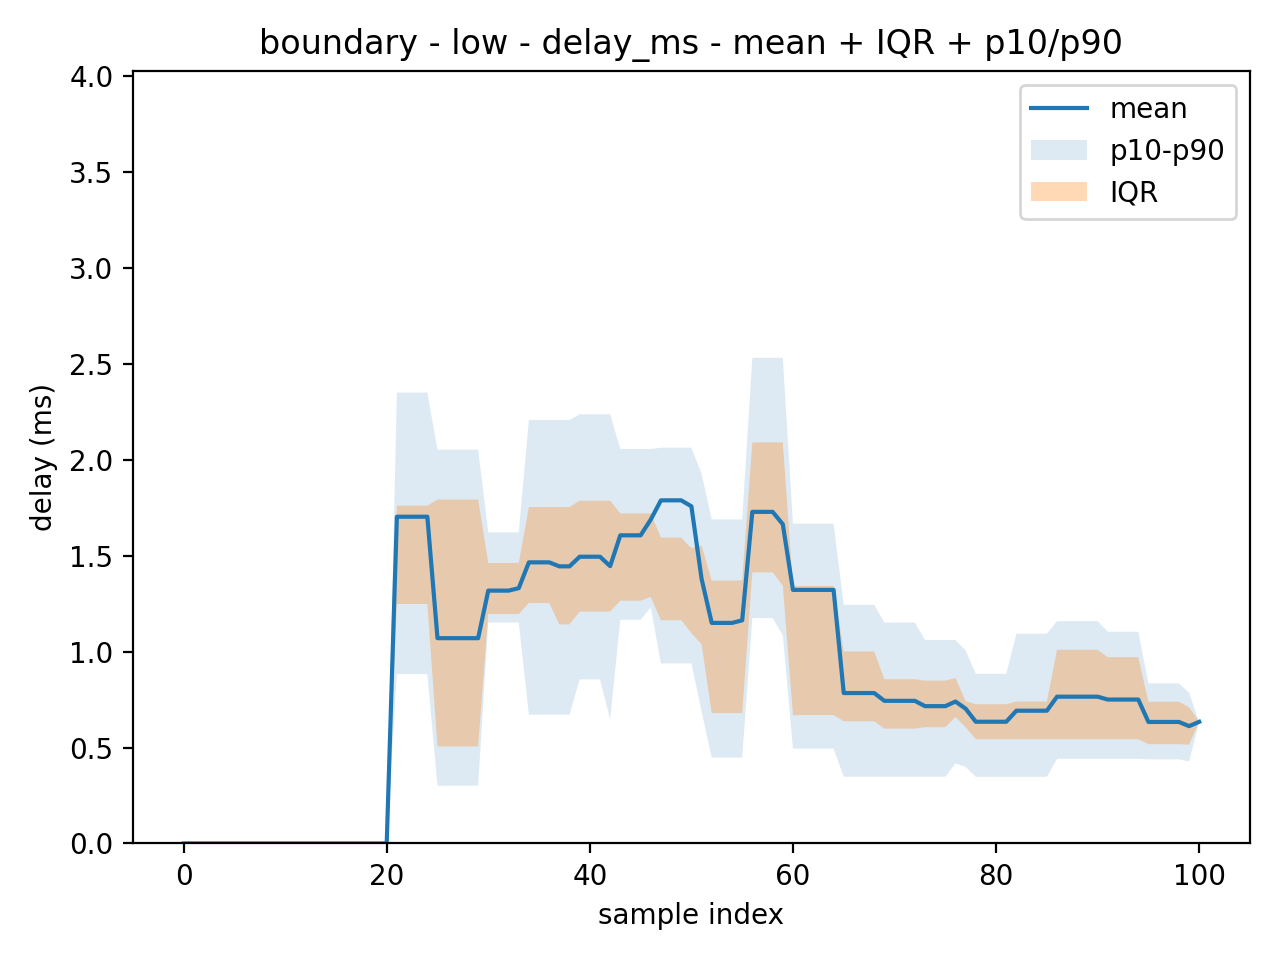
\includegraphics[width=\linewidth]{
      pars_plots/ntpsec/_aggregated/boundary/low/delay_ms_mean_iqr_p10_p90.png
    }
    \caption{Scenario LOW}
  \end{subfigure}
  \hfill
  \begin{subfigure}
    {0.32\textwidth}
    \centering
    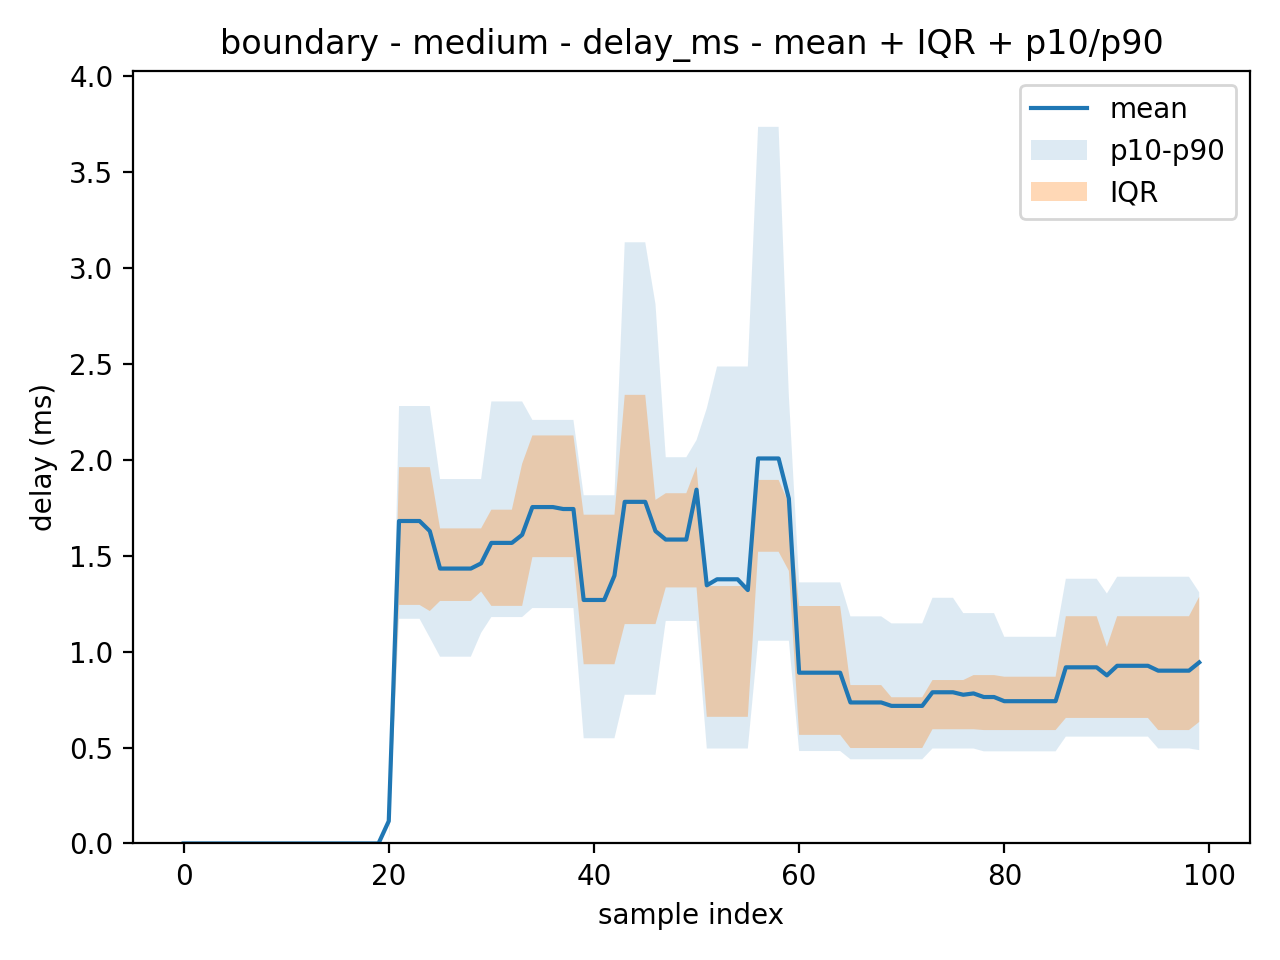
\includegraphics[width=\linewidth]{
      pars_plots/ntpsec/_aggregated/boundary/medium/delay_ms_mean_iqr_p10_p90.png
    }
    \caption{Scenario MEDIUM}
  \end{subfigure}
  \hfill
  \begin{subfigure}
    {0.32\textwidth}
    \centering
    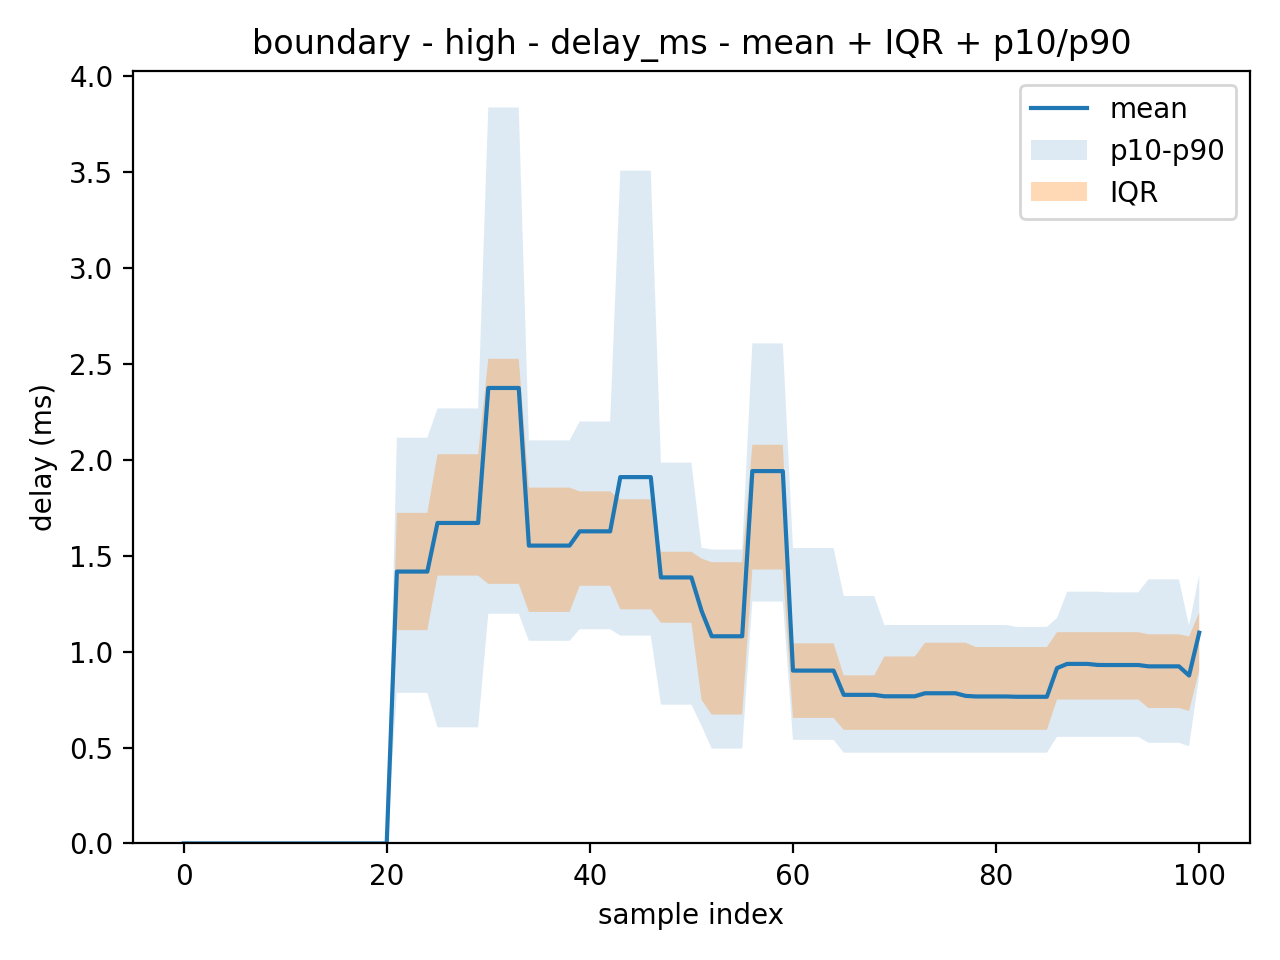
\includegraphics[width=\linewidth]{
      pars_plots/ntpsec/_aggregated/boundary/high/delay_ms_mean_iqr_p10_p90.png
    }
    \caption{Scenario HIGH}
  \end{subfigure}

  \caption{Media con banda inter-quartile e banda p10-p90 - nodo: \texttt{boundary}
  metrica: \texttt{delay}}
  \label{fig:scenario_comparison}
\end{figure}

\hrule

\begin{figure}[H]
  \centering

  \begin{subfigure}
    {0.32\textwidth}
    \centering
    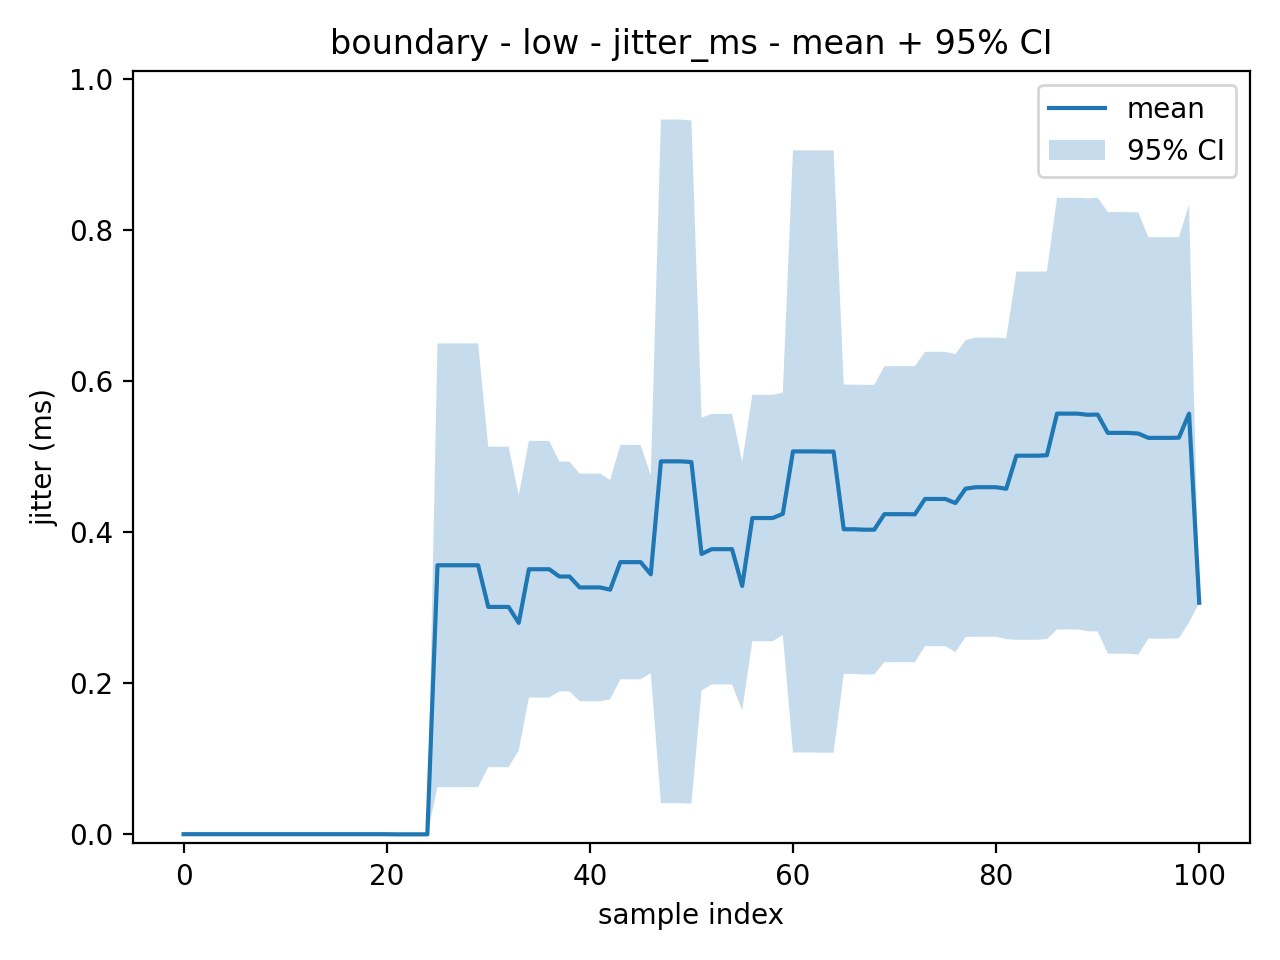
\includegraphics[width=\linewidth]{
      pars_plots/ntpsec/_aggregated/boundary/low/jitter_ms_mean_ci95.png
    }
    \caption{Scenario LOW}
  \end{subfigure}
  \hfill
  \begin{subfigure}
    {0.32\textwidth}
    \centering
    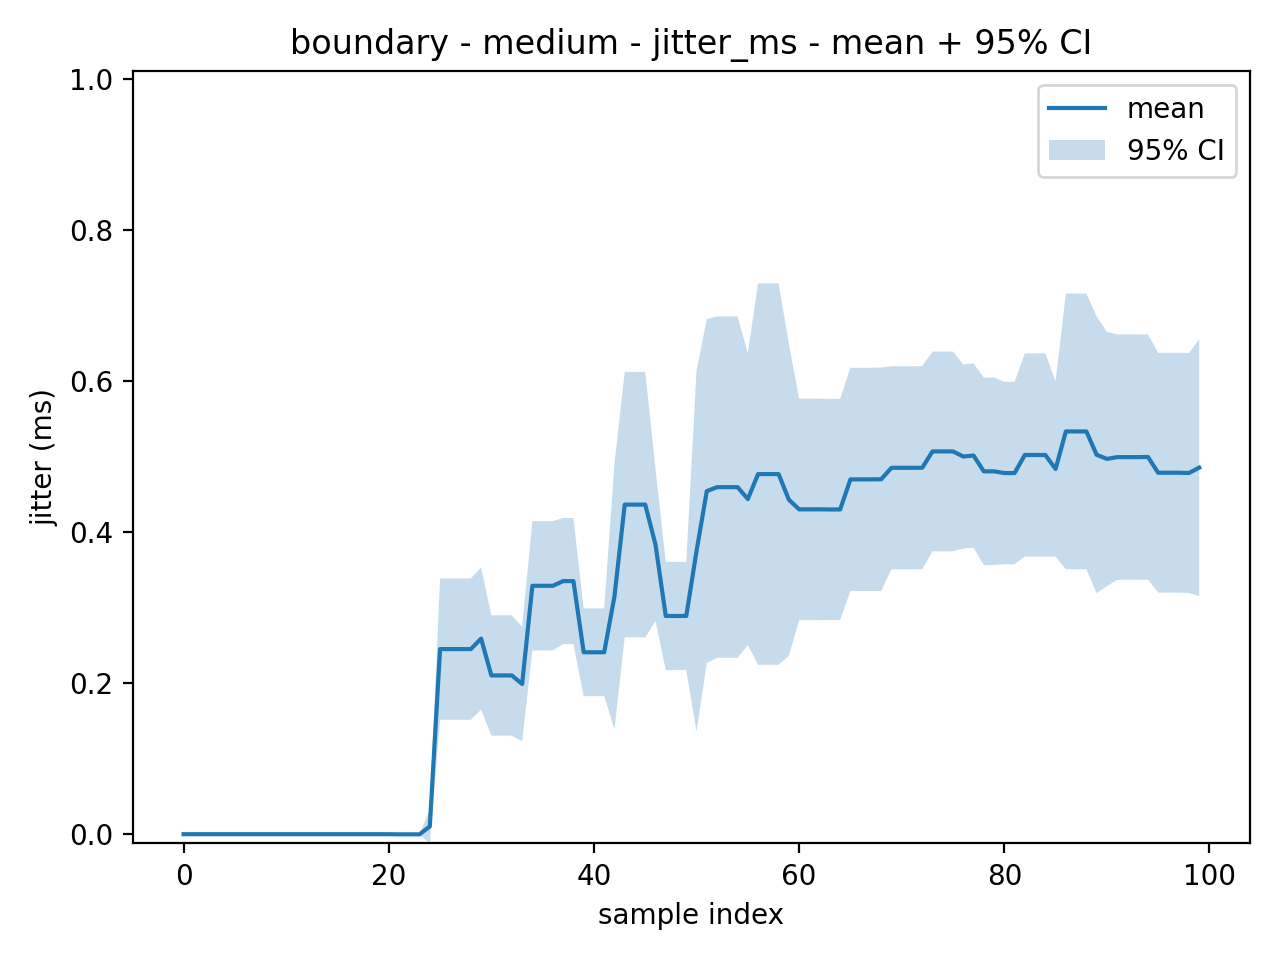
\includegraphics[width=\linewidth]{
      pars_plots/ntpsec/_aggregated/boundary/medium/jitter_ms_mean_ci95.png
    }
    \caption{Scenario MEDIUM}
  \end{subfigure}
  \hfill
  \begin{subfigure}
    {0.32\textwidth}
    \centering
    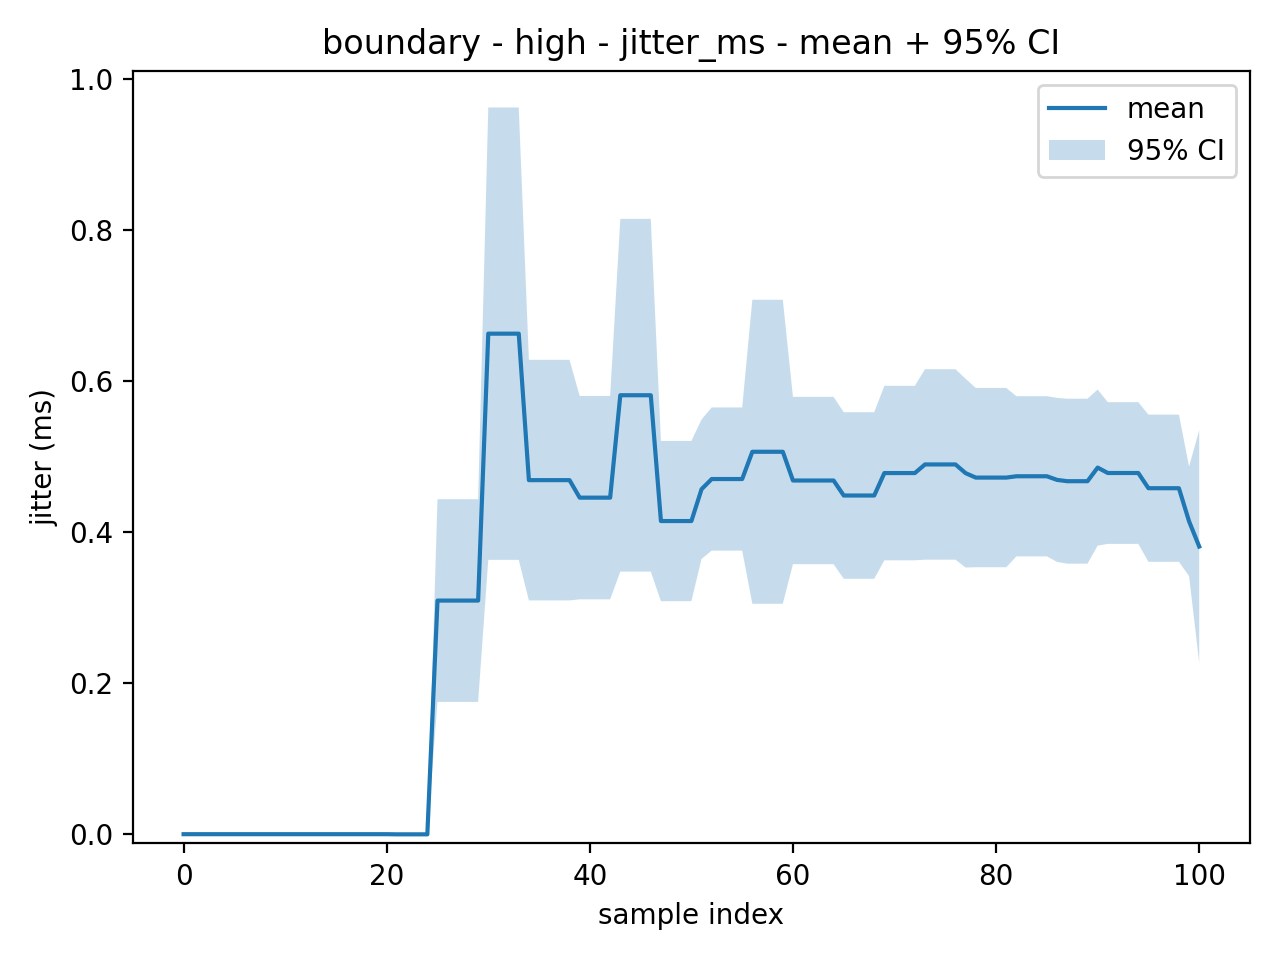
\includegraphics[width=\linewidth]{
      pars_plots/ntpsec/_aggregated/boundary/high/jitter_ms_mean_ci95.png
    }
    \caption{Scenario HIGH}
  \end{subfigure}

  \caption{Media con intervallo di confidenza al 95\% - nodo: \texttt{boundary} metrica:
  \texttt{jitter}}
  \label{fig:scenario_comparison}
\end{figure}
\begin{figure}[H]
  \centering

  \begin{subfigure}
    {0.32\textwidth}
    \centering
    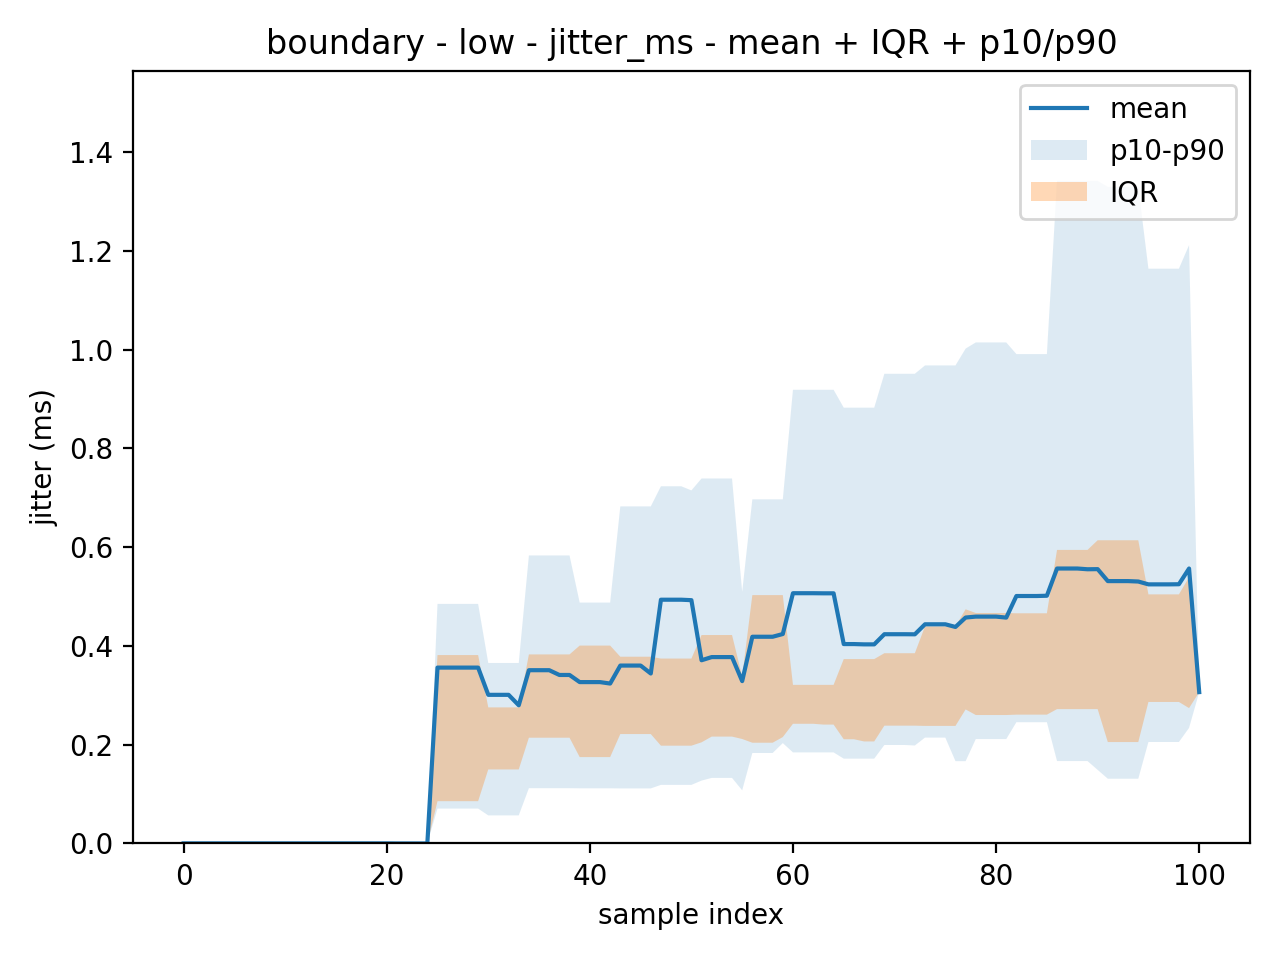
\includegraphics[width=\linewidth]{
      pars_plots/ntpsec/_aggregated/boundary/low/jitter_ms_mean_iqr_p10_p90.png
    }
    \caption{Scenario LOW}
  \end{subfigure}
  \hfill
  \begin{subfigure}
    {0.32\textwidth}
    \centering
    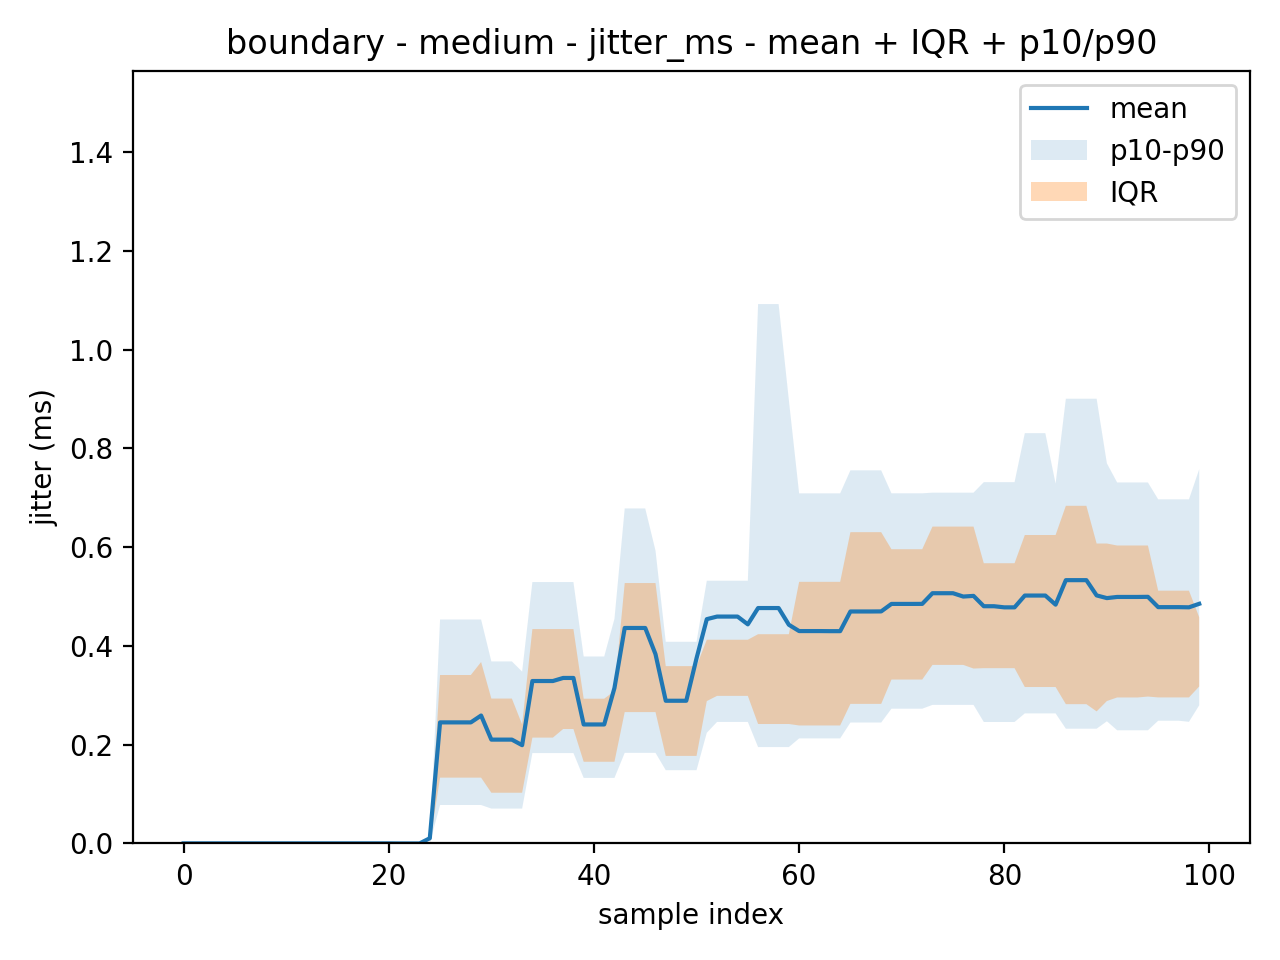
\includegraphics[width=\linewidth]{
      pars_plots/ntpsec/_aggregated/boundary/medium/jitter_ms_mean_iqr_p10_p90.png
    }
    \caption{Scenario MEDIUM}
  \end{subfigure}
  \hfill
  \begin{subfigure}
    {0.32\textwidth}
    \centering
    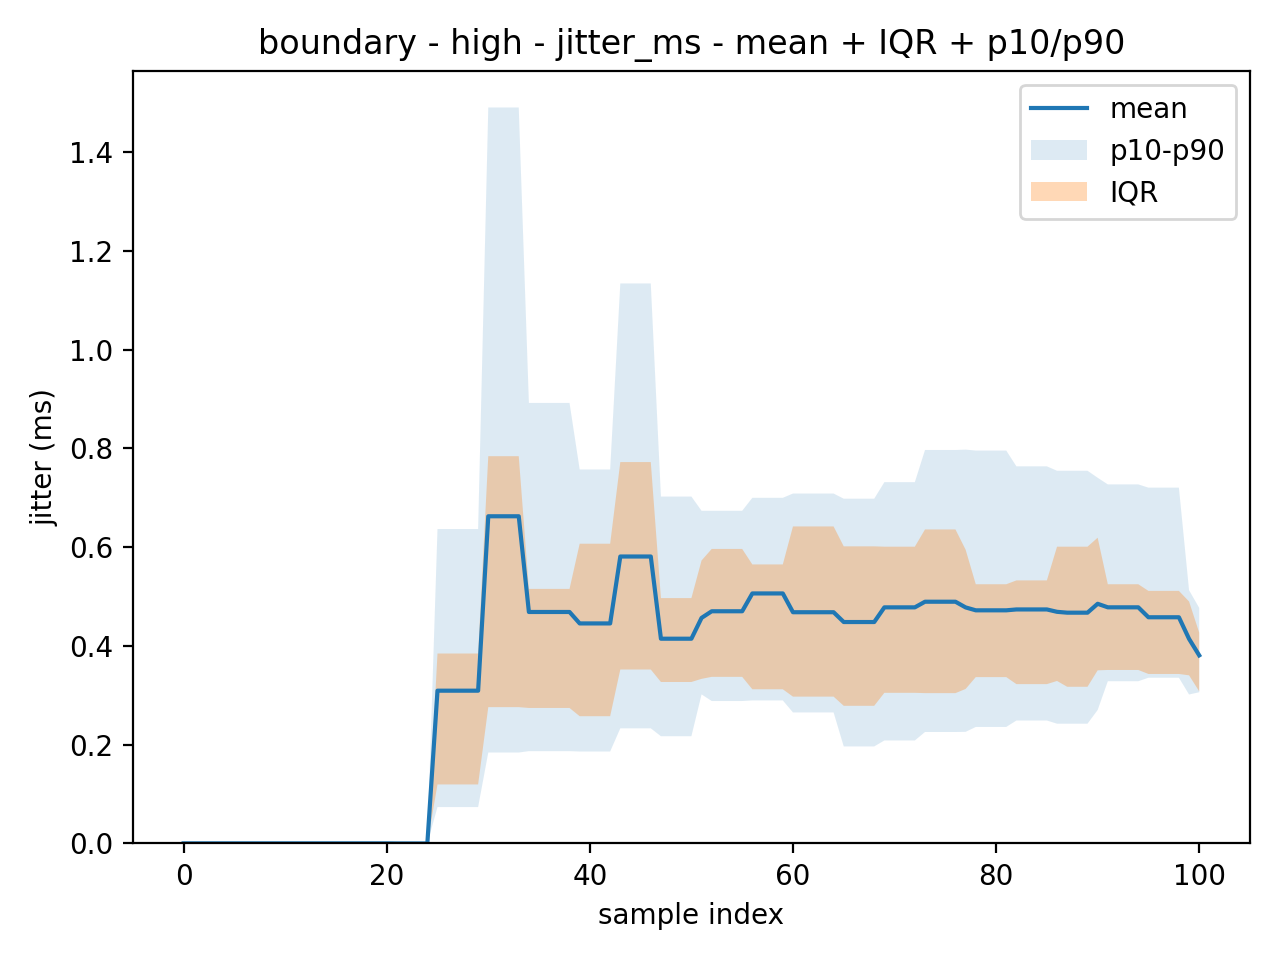
\includegraphics[width=\linewidth]{
      pars_plots/ntpsec/_aggregated/boundary/high/jitter_ms_mean_iqr_p10_p90.png
    }
    \caption{Scenario HIGH}
  \end{subfigure}

  \caption{Media con banda inter-quartile e banda p10-p90 - nodo: \texttt{boundary}
  metrica: \texttt{jitter}}
  \label{fig:scenario_comparison}
\end{figure}

\hrule

\begin{figure}[H]
  \centering

  \begin{subfigure}
    {0.32\textwidth}
    \centering
    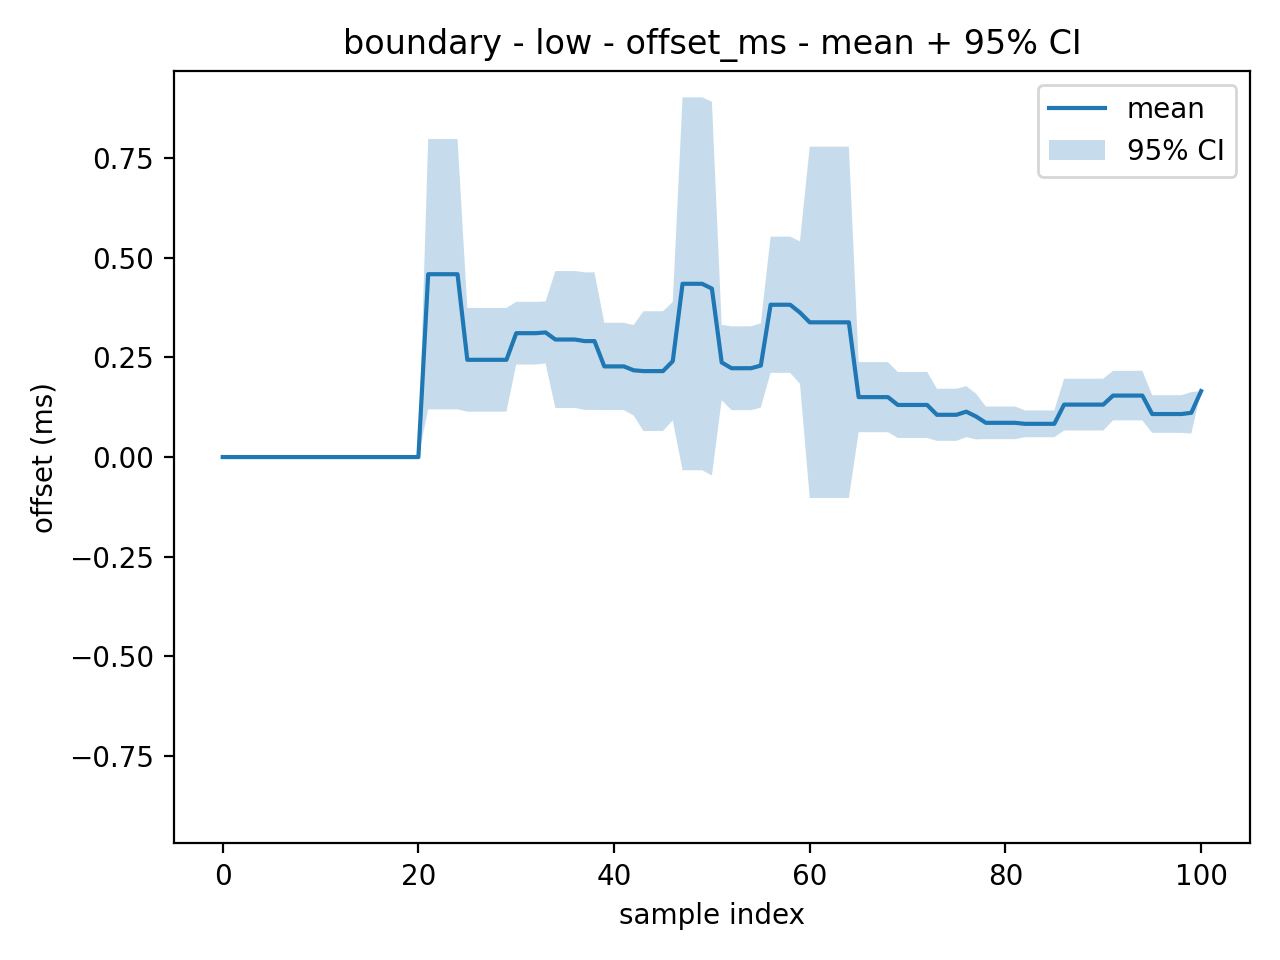
\includegraphics[width=\linewidth]{
      pars_plots/ntpsec/_aggregated/boundary/low/offset_ms_mean_ci95.png
    }
    \caption{Scenario LOW}
  \end{subfigure}
  \hfill
  \begin{subfigure}
    {0.32\textwidth}
    \centering
    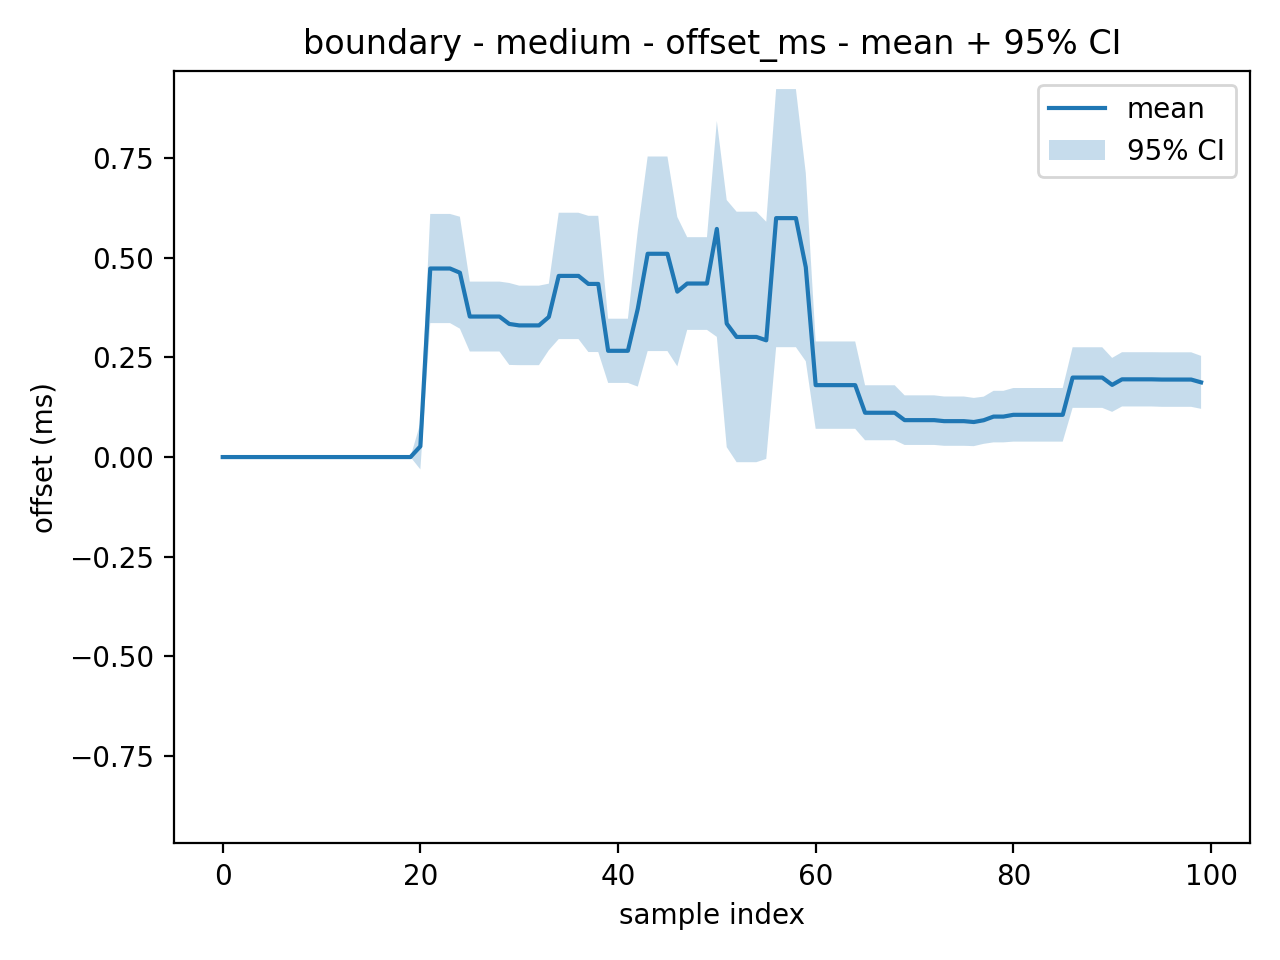
\includegraphics[width=\linewidth]{
      pars_plots/ntpsec/_aggregated/boundary/medium/offset_ms_mean_ci95.png
    }
    \caption{Scenario MEDIUM}
  \end{subfigure}
  \hfill
  \begin{subfigure}
    {0.32\textwidth}
    \centering
    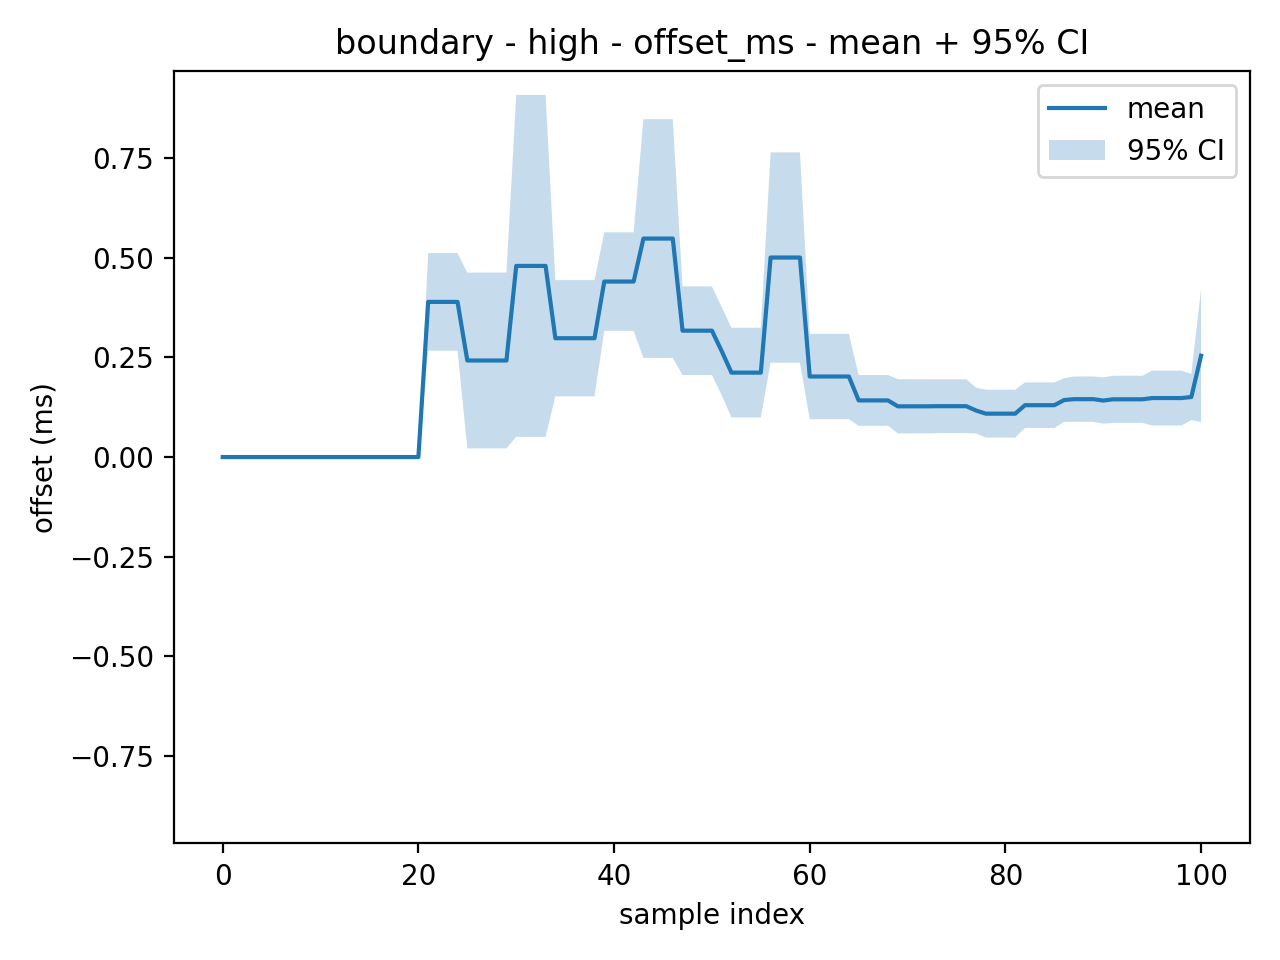
\includegraphics[width=\linewidth]{
      pars_plots/ntpsec/_aggregated/boundary/high/offset_ms_mean_ci95.png
    }
    \caption{Scenario HIGH}
  \end{subfigure}

  \caption{Media con intervallo di confidenza al 95\% - nodo: \texttt{boundary} metrica:
  \texttt{offset}}
  \label{fig:scenario_comparison}
\end{figure}
\begin{figure}[H]
  \centering

  \begin{subfigure}
    {0.32\textwidth}
    \centering
    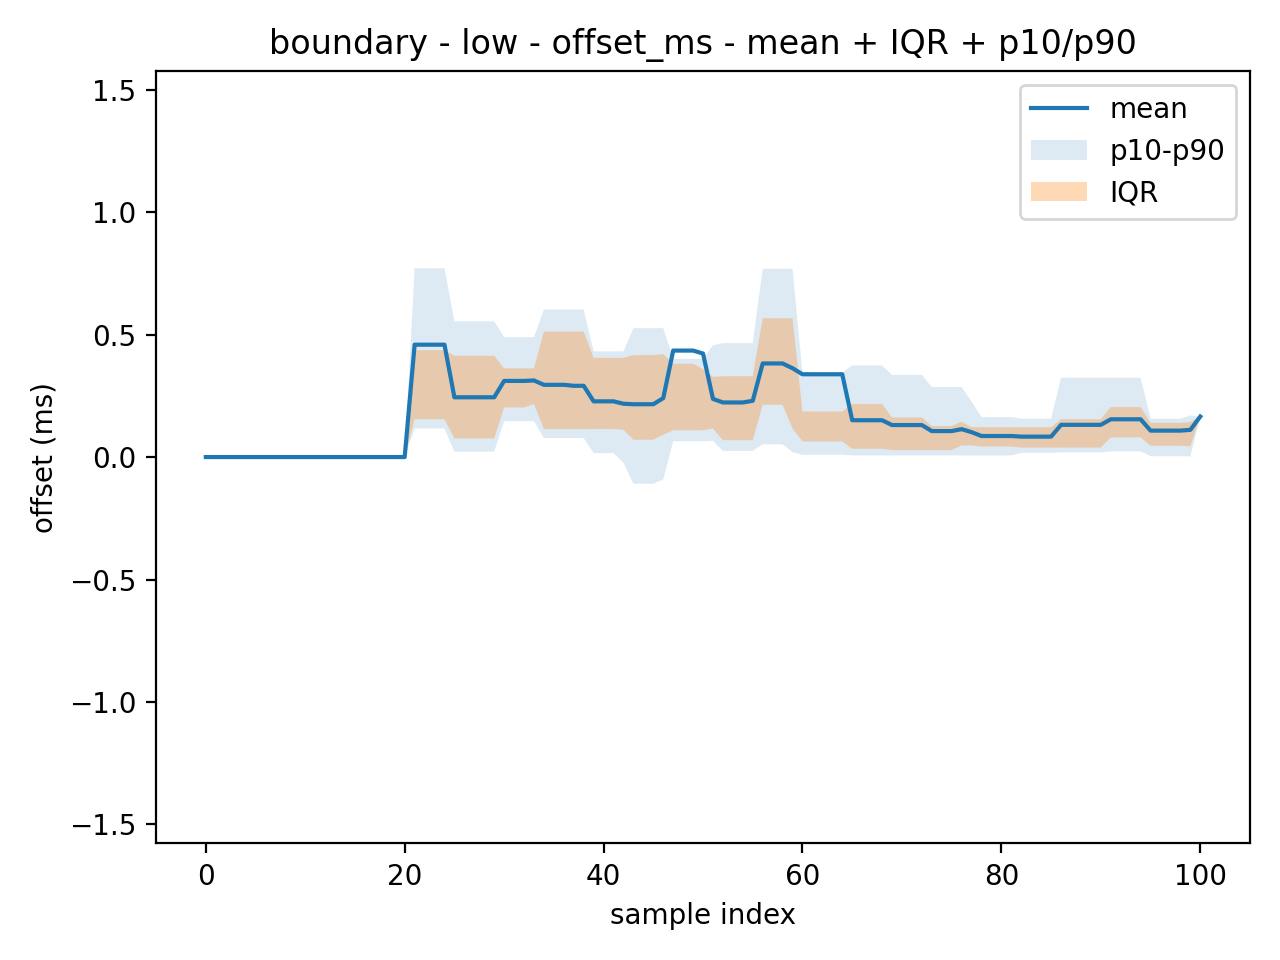
\includegraphics[width=\linewidth]{
      pars_plots/ntpsec/_aggregated/boundary/low/offset_ms_mean_iqr_p10_p90.png
    }
    \caption{Scenario LOW}
  \end{subfigure}
  \hfill
  \begin{subfigure}
    {0.32\textwidth}
    \centering
    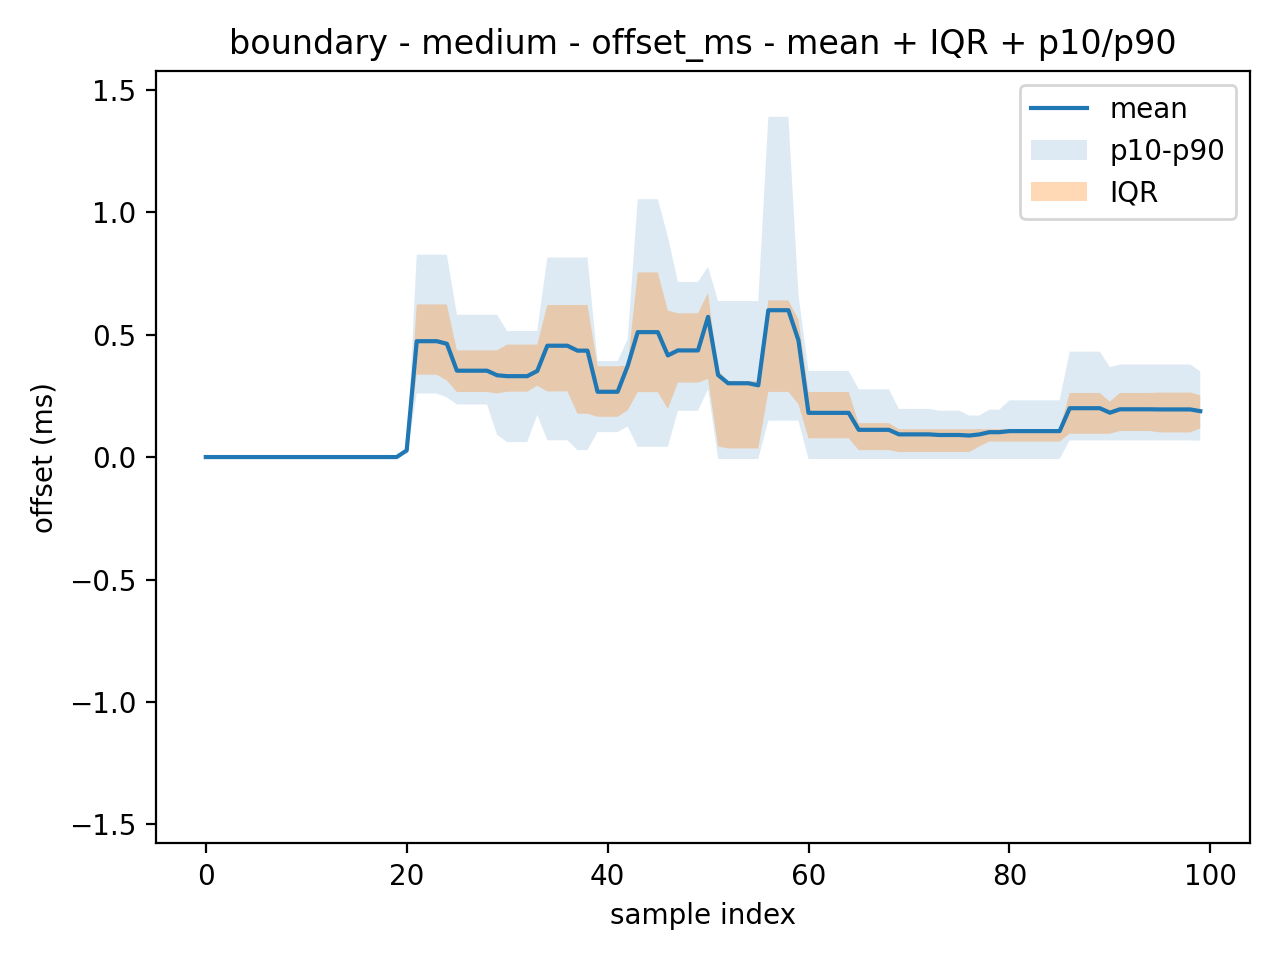
\includegraphics[width=\linewidth]{
      pars_plots/ntpsec/_aggregated/boundary/medium/offset_ms_mean_iqr_p10_p90.png
    }
    \caption{Scenario MEDIUM}
  \end{subfigure}
  \hfill
  \begin{subfigure}
    {0.32\textwidth}
    \centering
    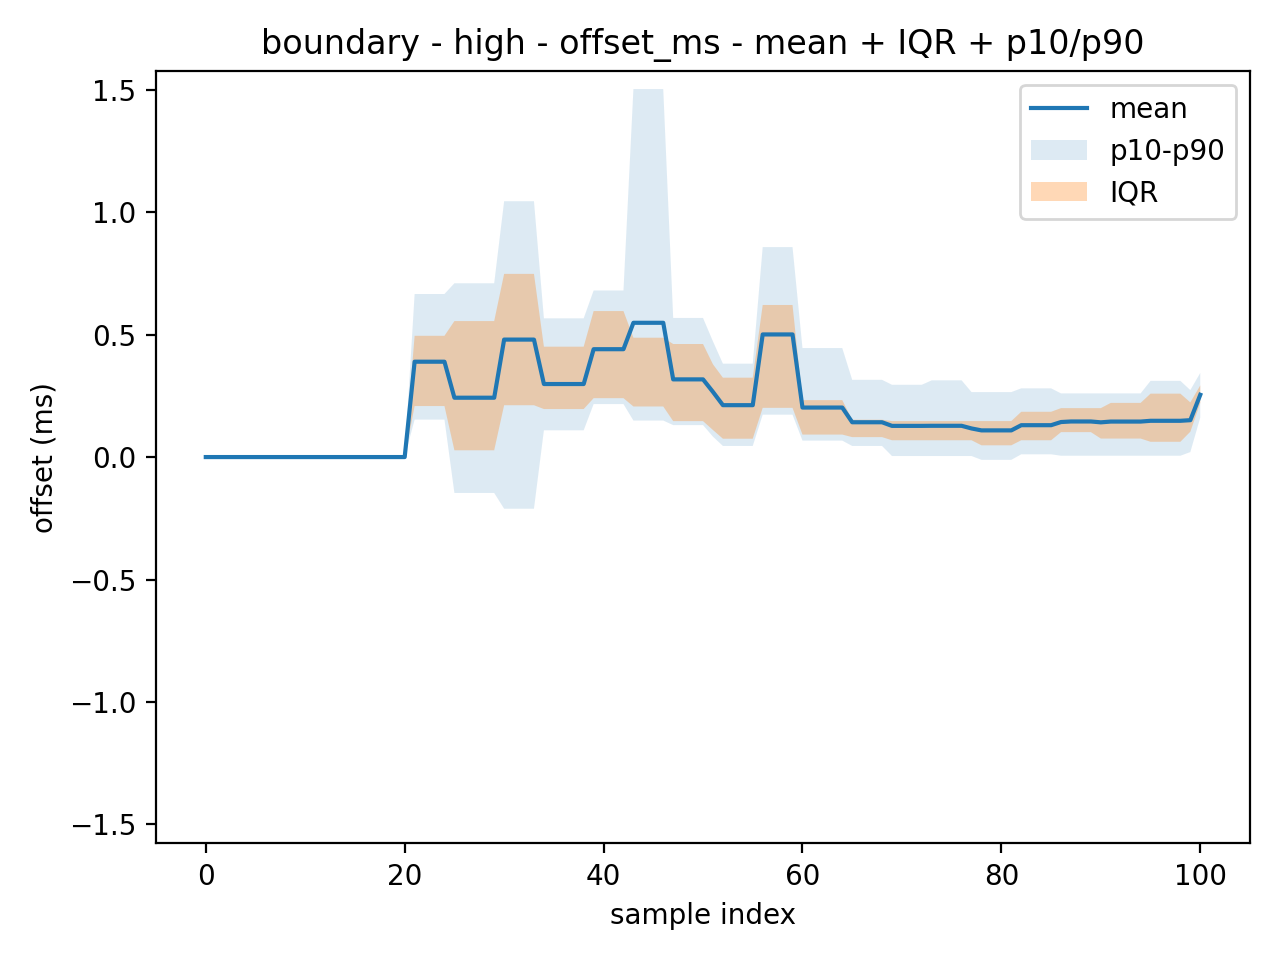
\includegraphics[width=\linewidth]{
      pars_plots/ntpsec/_aggregated/boundary/high/offset_ms_mean_iqr_p10_p90.png
    }
    \caption{Scenario HIGH}
  \end{subfigure}

  \caption{Media con banda inter-quartile e banda p10-p90 - nodo: \texttt{boundary}
  metrica: \texttt{offset}}
  \label{fig:scenario_comparison}
\end{figure}

Le metriche rilevate evidenziano un comportamento notevolmente differente
rispetto a quelle osservate sul nodo client. In tutti e tre gli scenari i dati restano
coerenti e stabili, con valori dello stesso ordine di grandezza, non evidenziando
una crescita progressiva netta al crescere della severità degli impairment di rete.
Vi è coerenza con la premessa iniziale.

Il delay ha valori medi di ~1.080 ms nello scenario low, ~1.139 ms nello scenario
medium e ~1.127 ms nello scenario high. Variazioni minime che non configurano un cambio
di regime. La dispersione associata conferma le ipotesi, con metriche dello stesso
ordine di grandezza.

Andamento analogo è osservabile per il jitter. I valori medi sono di circa 0.446
ms in low, 0.442 ms in medium e 0.473 ms in high. Differenze ridotte, evidenziando
un'assenza di degrado del nodo \texttt{boundary}.La variabilità delle curve
aggregate resta limitata, suggerendo un comportamento omogeneo nei tre casi.

Infine l'offset, con valori anche essi contenuti in tutti gli scenari. La media di
~0.204 ms nel caso low, 0.254 ms nel caso medium e 0.236 ms nel caso high.
Comportamento invariato, anche per la dispersione, con minime oscillazioni
compatibili con l'ambiente sperimentale, ma non un andamento monotono né un incremento
compatibile con un peggioramento strutturale.

I risultati ottenuti mostrano quindi un assenza di degrado. Le differenze
osservate tra low, medium e high risultano contenute e prive di una tendenza sistematica,
confermando l'ipotesi iniziale.

\section{\texttt{ptp4l}}
L'analisi dei dati relativa al demone \texttt{\textbf{ptp4l}} è fatta su due nodi
della topologia. In particolare sui nodi \texttt{clientptp} e \texttt{boundary}, per
i quali sono disponibili misurazioni direttamente riconducibili al comportamento del
protocollo in termini di sincronizzazione e ritardo.

Il nodo \texttt{servergm}, per configurazione, essendo eletto definitivamente GM,
non fornisce metriche comparabili, poiché il relativo output è limitato
essenzialmente allo stato di inizializzazione del demone e alla selezione del
clock locale come \texttt{best master}, non viene quindi incluso nell'analisi.

Anche in questa situazione \texttt{\textbf{ptp4l}}, gli impairment di rete
introdotti mediante \texttt{tc/netem} sono applicati sul ramo \texttt{downstream}
a valle del nodo \texttt{boundary}. Di conseguenza il confronto tra scenari
assume significato principalmente nel caso del nodo \texttt{clientptp}. Per
quanto riguarda il nodo \texttt{boundary} ci si attende, in linea teorica, un impatto
più contenuto, o una totale assenza di degrado.

Alla luce di ciò, l'analisi viene sviluppata separatamente per i nodi \texttt{clientptp}
e \texttt{boundary}.

\subsection{\texttt{clientptp}}
Per quanto riguarda, l'analisi quantitativa delle metriche, non può essere estesa
in modo uniforme a tutti gli scenari. Infatti, nello scenario \texttt{high} non
venendo raggiunta una stabile condizione operativa i campioni prodotti non sono
utilizzabili per un confronto. Quindi l'analisi si limita agli scenari \texttt{low}
e \texttt{medium}.

L'instabilità non raggiunta è evidenziata dal file di log, il quale mostra
ripetute selezioni del clock locale come miglior master e un solo tentativo
transitorio di passaggio verso un master esterno, seguito tuttavia da ritorno allo
stato di \texttt{LISTENING}. L'assenza di campioni numerici confrontabili nello scenario
\texttt{high} rappresenta dunque un risultato sperimentale, e segnala un livello di
degrado tale da impedire la normale operatività del client PTP. Il relativo
output viene comunque richiamato a supporto di tale evidenza qualitativa.

\subsubsection{Analisi metrica: \texttt{path Delay}}
\begin{figure}[H]
  \centering

  \begin{subfigure}
    {0.4\textwidth}
    \centering
    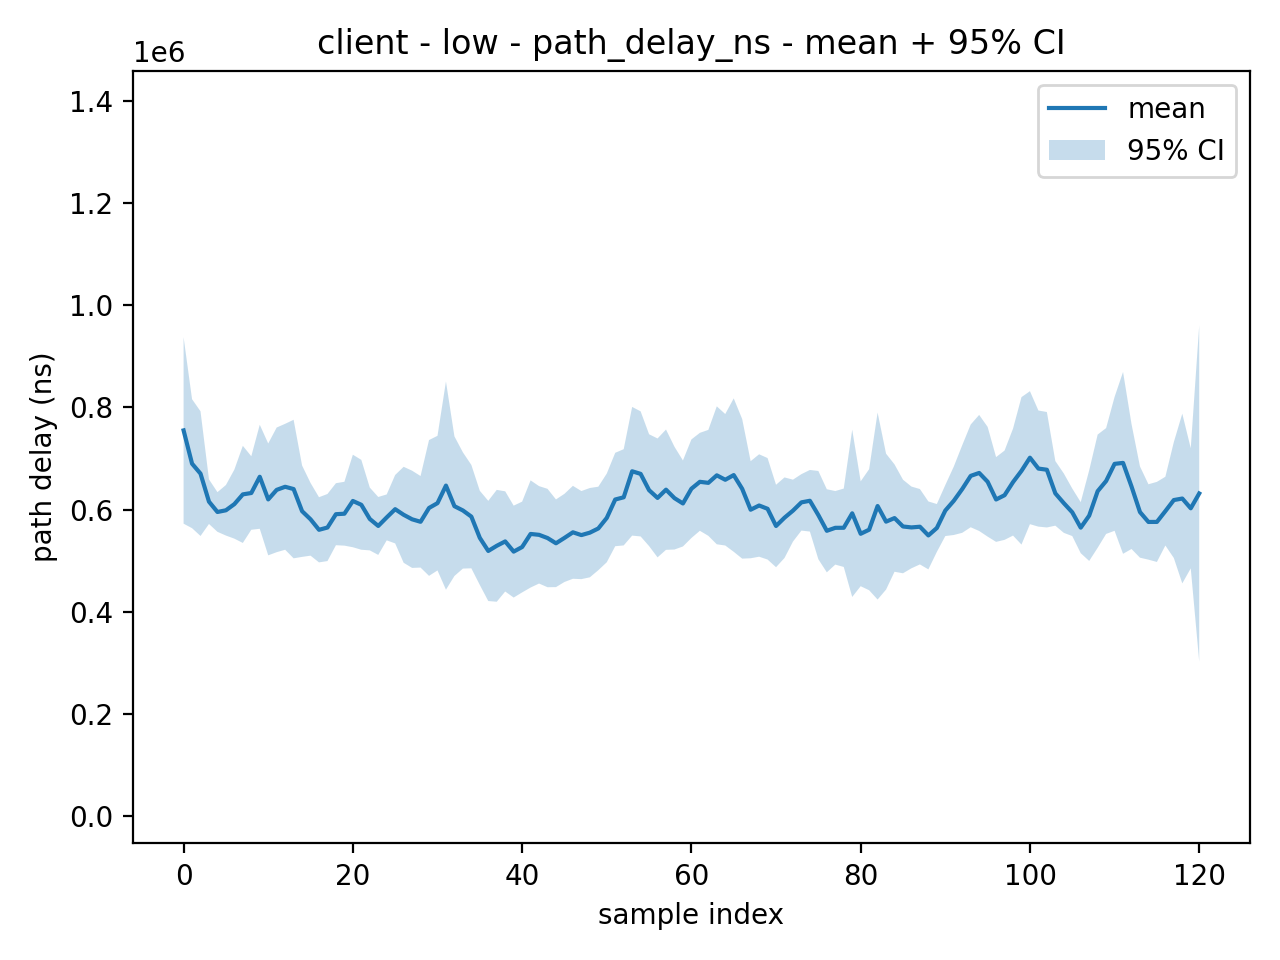
\includegraphics[width=\linewidth]{
      pars_plots/ptp/_aggregated/client/low/path_delay_ns_mean_ci95.png
    }
    \caption{Scenario LOW}
  \end{subfigure}
  \hfill
  \begin{subfigure}
    {0.4\textwidth}
    \centering
    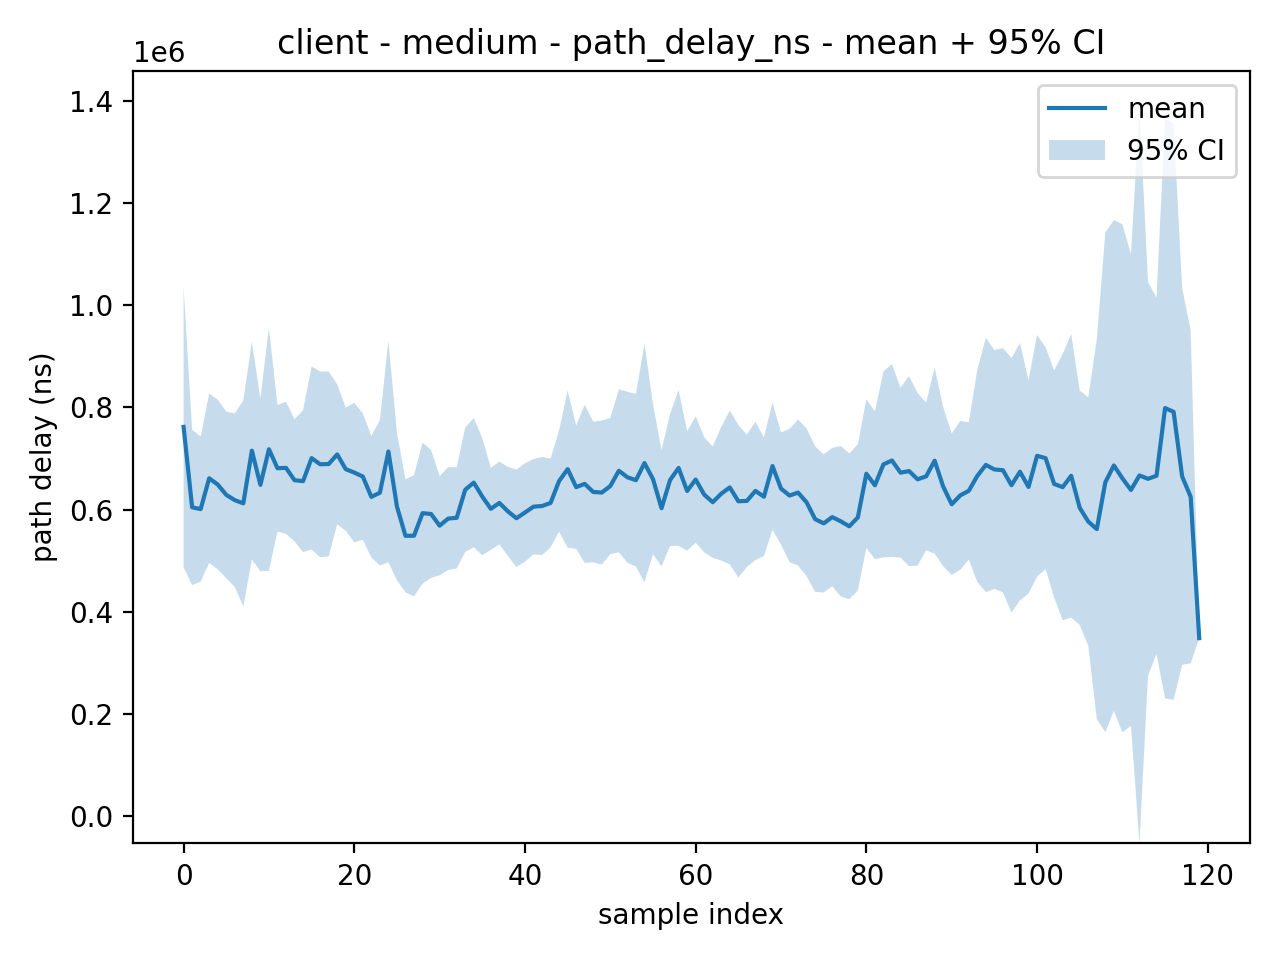
\includegraphics[width=\linewidth]{
      pars_plots/ptp/_aggregated/client/medium/path_delay_ns_mean_ci95.png
    }
    \caption{Scenario MEDIUM}
  \end{subfigure}
  \caption{Media con intervallo di confidenza al 95\% - nodo: \texttt{clientptp}}
  \label{fig:scenario_comparison}
\end{figure}
\begin{figure}[H]
  \centering

  \begin{subfigure}
    {0.4\textwidth}
    \centering
    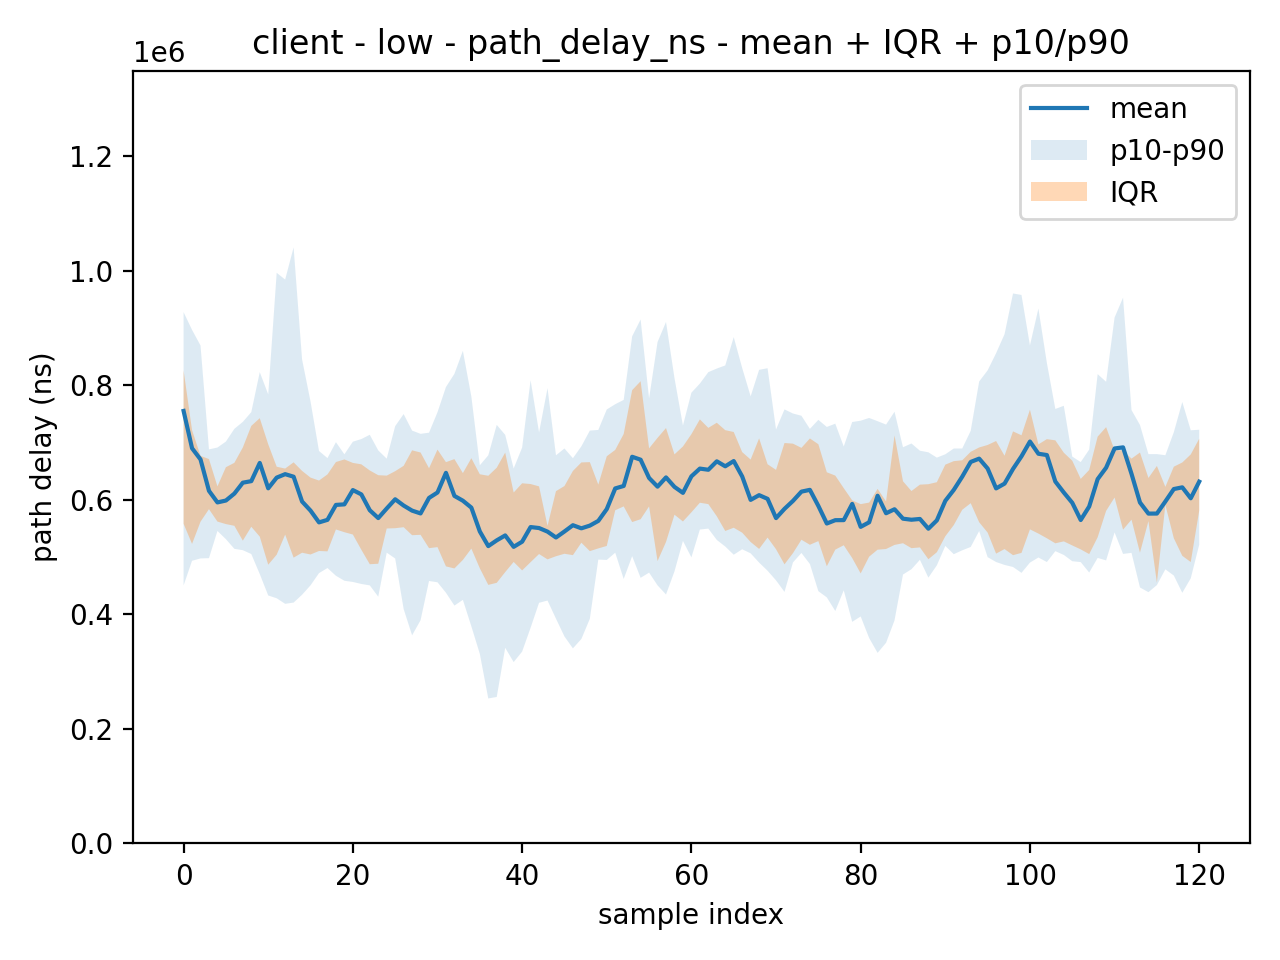
\includegraphics[width=\linewidth]{
      pars_plots/ptp/_aggregated/client/low/path_delay_ns_mean_iqr_p10_p90.png
    }
    \caption{Scenario LOW}
  \end{subfigure}
  \hfill
  \begin{subfigure}
    {0.4\textwidth}
    \centering
    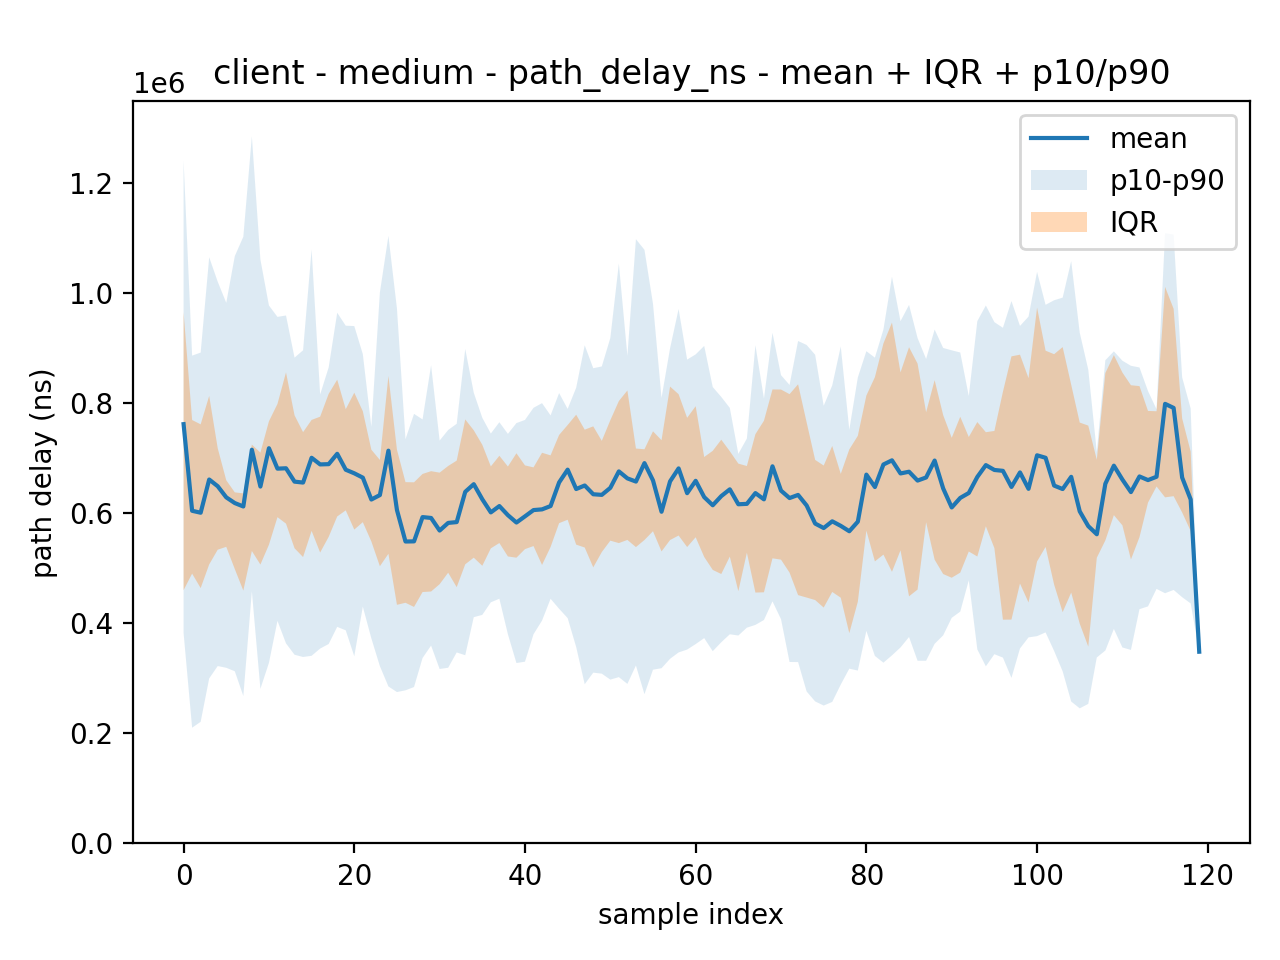
\includegraphics[width=\linewidth]{
      pars_plots/ptp/_aggregated/client/medium/path_delay_ns_mean_iqr_p10_p90.png
    }
    \caption{Scenario MEDIUM}
  \end{subfigure}
  \caption{Media con banda inter-quartile e banda p10-p90 - nodo: \texttt{clientptp}}
  \label{fig:scenario_comparison}
\end{figure}

La metrica \texttt{path delay} sul nodo \texttt{clientptp} consente di valutare il
ritardo stimato lungo il percorso di sincronizzazione tra il client e il master.

Nello scenario \texttt{low} vi è un andamento mediamente regolare, collocandosi su
valori nell'ordine di centinaia di microsecondi. La curva aggregata ha un valore
medio ~$606.8\,\mu s$ e la mediana è di ~$602.5\,\mu s$. La distribuzione dei valori
centrali è piuttosto contenuta, con il primo e terzo quartile rispettivamente a
$575.8\,\mu s$ e $638.6\,\mu s$. L'analisi dei grafici conferma un andamento stabile,
pur con oscillazioni locali non trascurabili, ma complessivamente compatibili con
una condizione di rete moderatamente controllata.

Nel caso \texttt{medium}, si ha un livello medio crescente ma sempre contenuto.
La curva aggregata ha un valore medio di ~$6 42.2\,\mu s$, con mediana pari a ~$6
45 .5\,\mu s$. L'incremento rispetto allo scenario precedente è nell'ordine di
decine di microsecondi. Questo scenario, comunque, mostra una dispersione più elevata.
Il primo e il terzo quartile della curva centrale sono rispettivamente pari a
$613.0\,\mu s$ e $672.3\, \mu s$, invece le bande di variabilità sono mediamente più
ampie. L'ampiezza dell'IQR, cosi come quella della fascia $p10$--$p 90$, segnalano una
minore regolarità della stima del ritardo di percorso.

Vi è un chiaro aumento del degrado tra i primi due scenari, in termini di misurazioni
ottenute. Nonostante il degrado della rete non produce un forte aumento del
valore medio del \texttt{path delay}, ma si riflette soprattutto in una maggiore
variabilità delle misurazioni. La metrica risulta quindi sensibile al peggioramento
dello scenario sperimentale, ma l'effetto osservato si manifesta principalmente
come perdita di stabilità più che come incremento netto del livello centrale. Lo scenario
\texttt{high}, come già discusso, evidenzia una totale perdita di connessione
con il riferimento principale.

\subsubsection{Analisi metrica: \texttt{RMS offset}}
\begin{figure}[H]
  \centering

  \begin{subfigure}
    {0.4\textwidth}
    \centering
    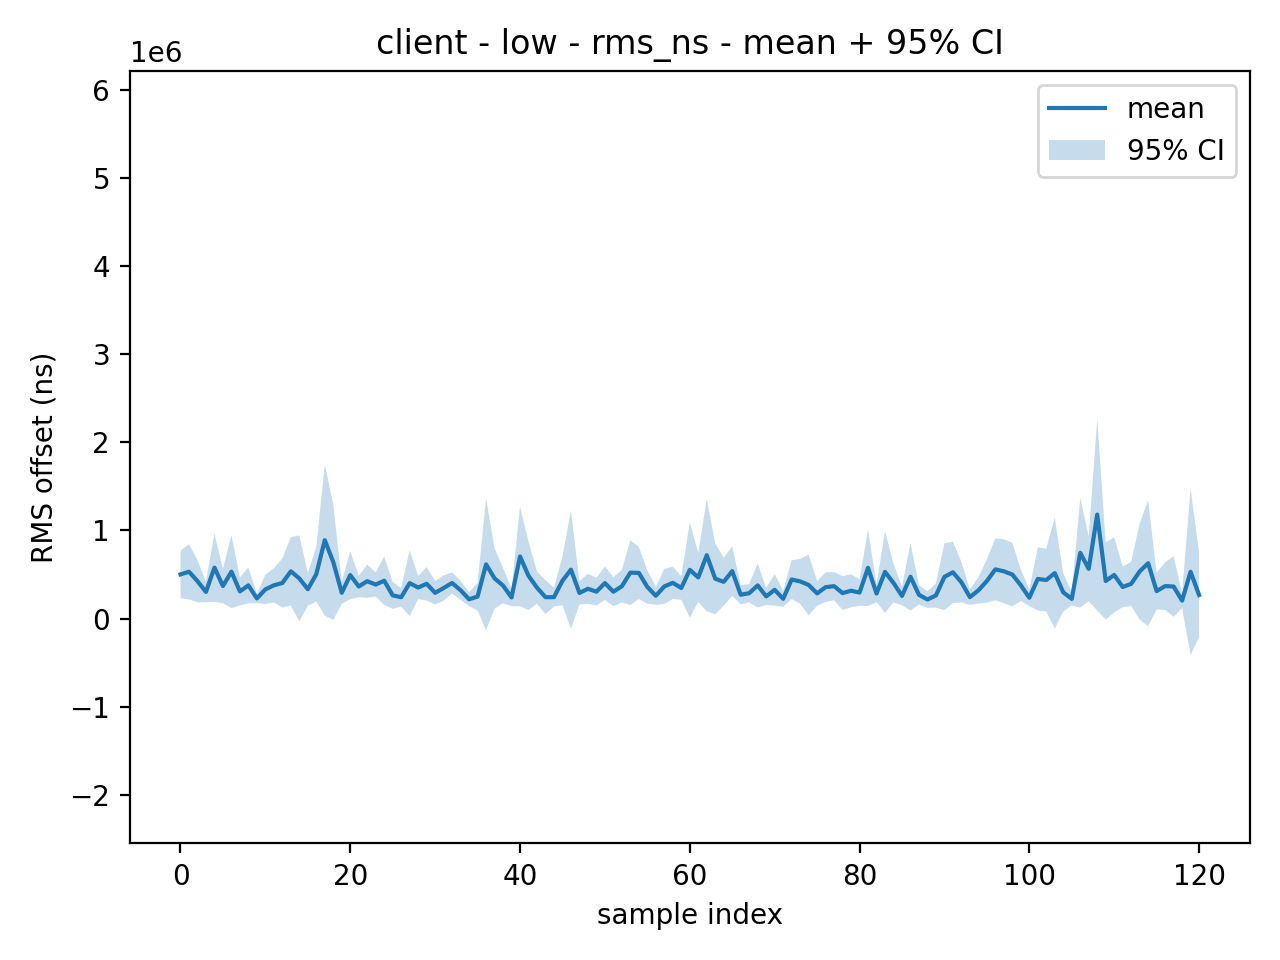
\includegraphics[width=\linewidth]{
      pars_plots/ptp/_aggregated/client/low/rms_ns_mean_ci95.png
    }
    \caption{Scenario LOW}
  \end{subfigure}
  \hfill
  \begin{subfigure}
    {0.4\textwidth}
    \centering
    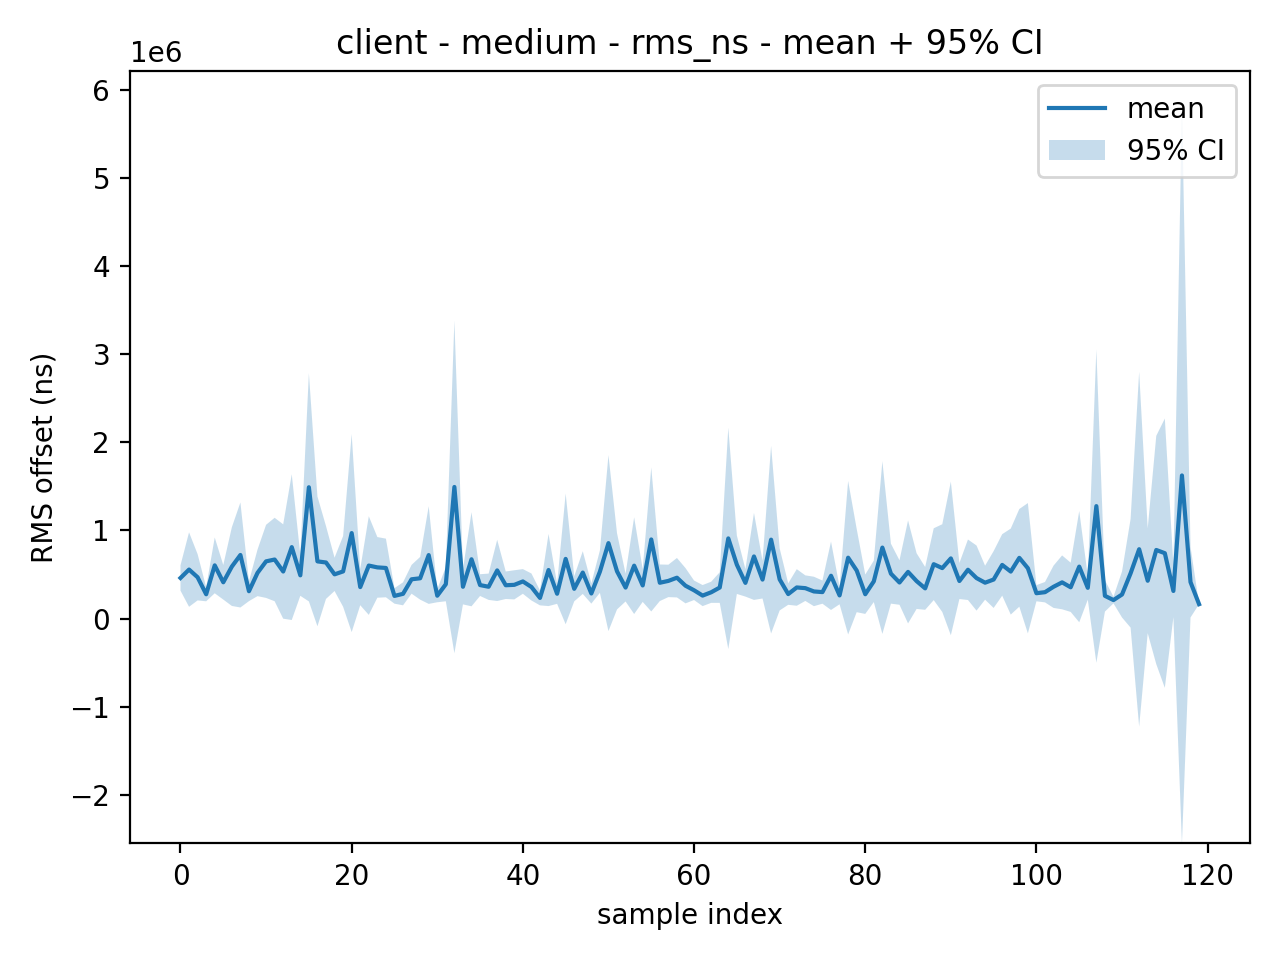
\includegraphics[width=\linewidth]{
      pars_plots/ptp/_aggregated/client/medium/rms_ns_mean_ci95.png
    }
    \caption{Scenario MEDIUM}
  \end{subfigure}
  \caption{Media con intervallo di confidenza al 95\% - nodo: \texttt{clientptp}}
  \label{fig:scenario_comparison}
\end{figure}
\begin{figure}[H]
  \centering

  \begin{subfigure}
    {0.4\textwidth}
    \centering
    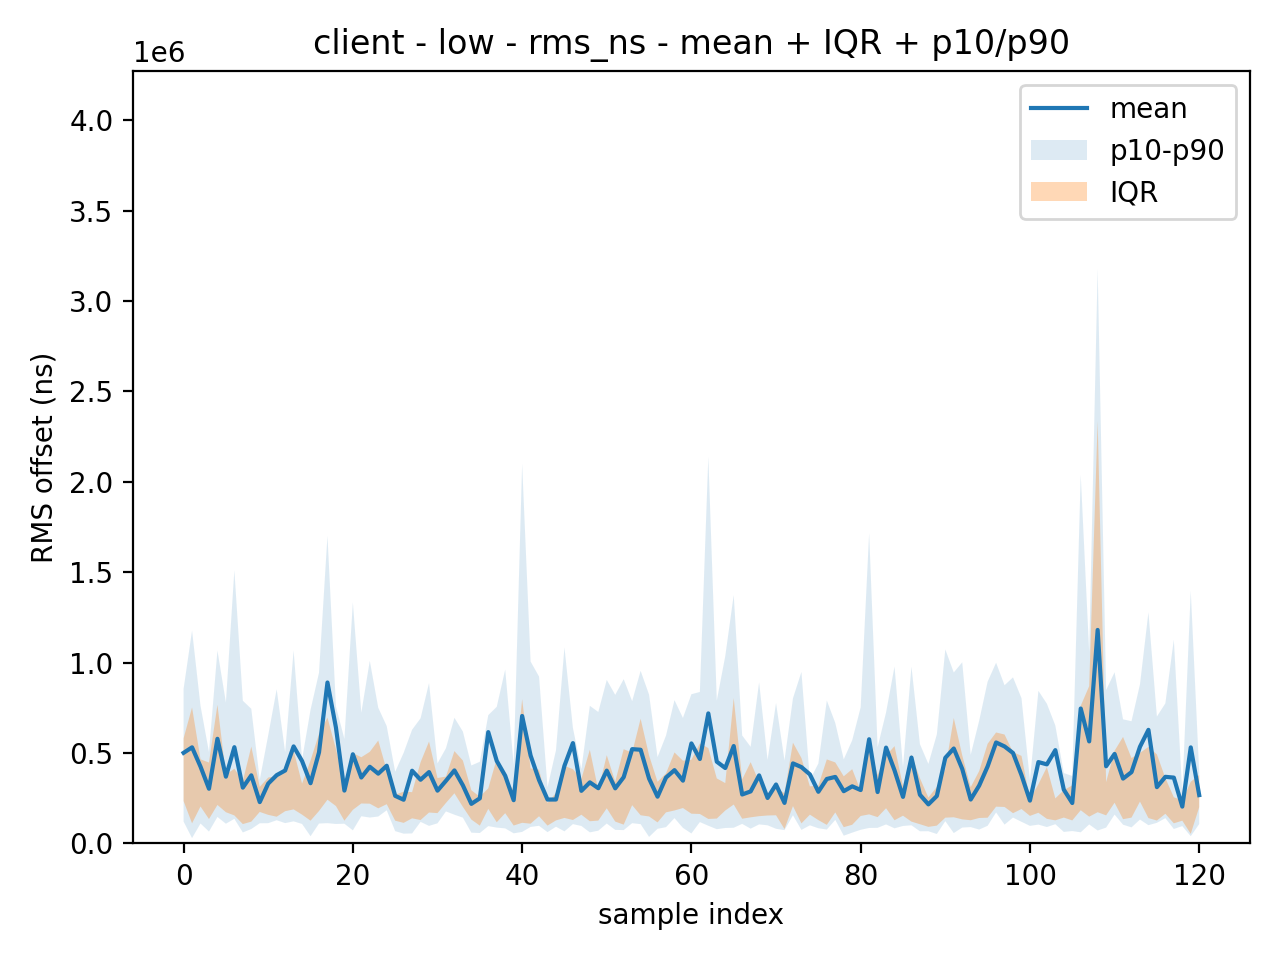
\includegraphics[width=\linewidth]{
      pars_plots/ptp/_aggregated/client/low/rms_ns_mean_iqr_p10_p90.png
    }
    \caption{Scenario LOW}
  \end{subfigure}
  \hfill
  \begin{subfigure}
    {0.4\textwidth}
    \centering
    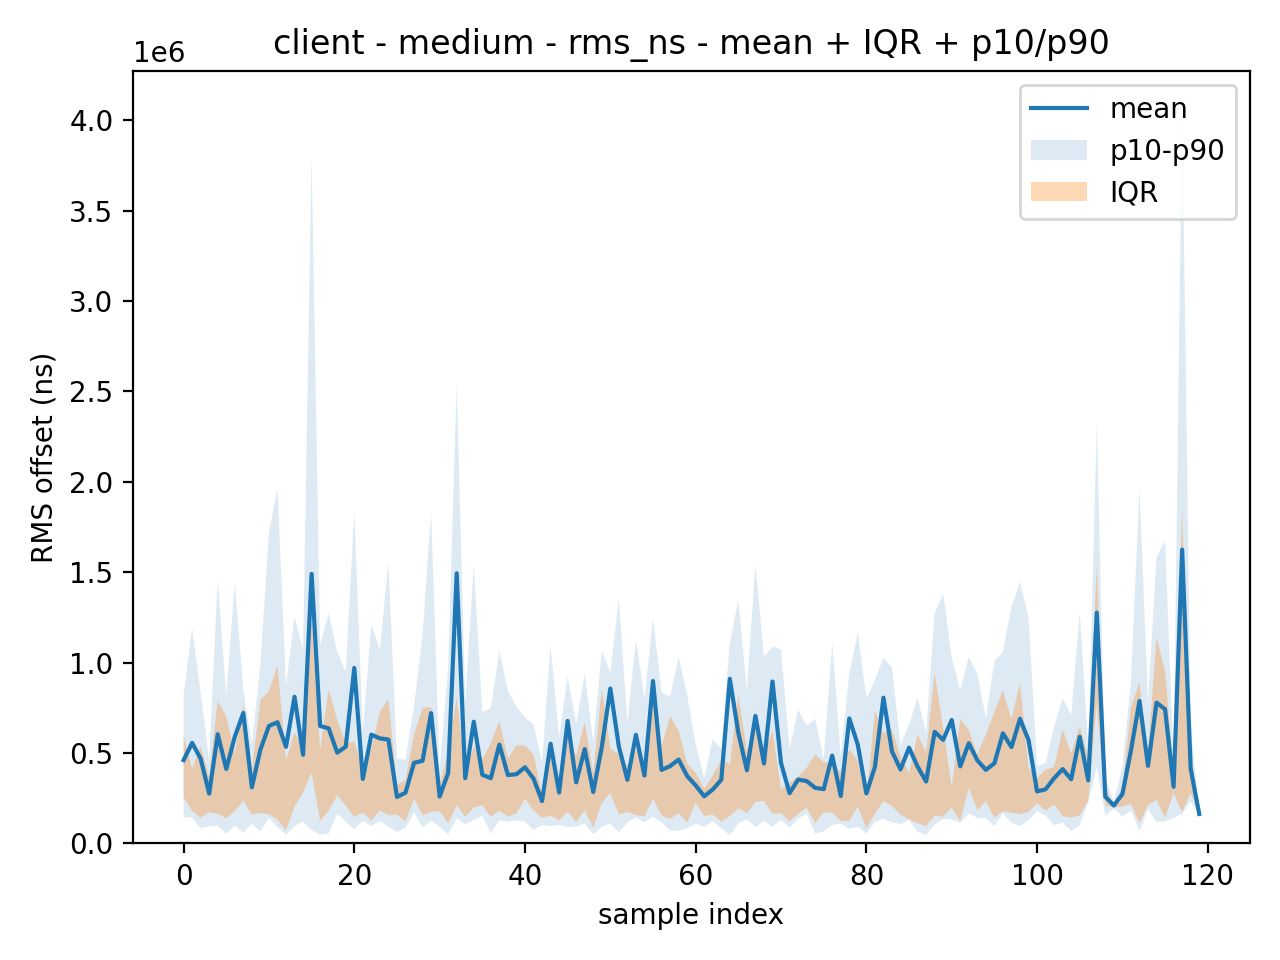
\includegraphics[width=\linewidth]{
      pars_plots/ptp/_aggregated/client/medium/rms_ns_mean_iqr_p10_p90.png
    }
    \caption{Scenario MEDIUM}
  \end{subfigure}
  \caption{Media con banda inter-quartile e banda p10-p90 - nodo: \texttt{clientptp}}
  \label{fig:scenario_comparison}
\end{figure}

La metrica \texttt{RMS} sul nodo \texttt{clientptp} misura l'entità media dell'errore
di sincronizzazione osservato dal client PTP fornendo una misura della qualità temporale
raggiunta dal nodo nel corso dell'esperimento.

Nello scenario \texttt{low}, i valori medi sono nell'ordine di alcune centinaia di
microsecondi. Il valore medio della curva aggregata è di ~$406.7\,\mu s$, mentre
la mediana è ~$378.1\,\mu s$. La distribuzione dei valori centrali è nell'intervallo
$3 02.5\,\mu s$ e $493.2\,\mu s$, con presenza di picchi locali più elevati.
L'andamento della serie risulta nel complesso irregolare ma ancora contenuto.

Nello scenario \texttt{medium}, la RMS aumenta. Il valore medio della curva aggregata
si attesta a ~$514.9\,\mu s$. La mediana ha un valore di ~$458.5\,\mu s$. Rispetto
allo scenario \texttt{low} vi è un incremento sensibile pari a poco più di
$100\,\mu s$. L'aspetto però più rilevante è rappresentato dall'aumento della dispersione.
L'intervallo inter-quartile dei valori centrali è maggiore e le bande di
variabilità nei grafici risultano più estese. In generale la serie mostra una maggiore
oscillazione.

In generale, la metrica RMS mostra un marcato peggioramento al passaggio dallo
scenario \texttt{low} a quello \texttt{medium}. A differenza di quanto osservato sul
\texttt{path delay} vi è anche un incremento maggiore del livello medio
dell'errore temporale. Per lo scenario \texttt{high} vale sempre la premessa
iniziale, confermando l'eccessivo degrado di rete che non permette a \texttt{clientptp}
di stabilizzarsi.

\subsection{\texttt{boundary}}
L'analisi sul nodo \texttt{boundary} è simmetrica a quella effettuata con il demone
\texttt{NTPsec}. Le metriche osservate in questo caso descrivono infatti il comportamento
della sincronizzazione del boundary rispetto al \texttt{master upstream} (\texttt{servergm}).
Non essendoci impairment di rete direttamente applicati, in linea teorica, non
ci si attende un degrado strutturale. A sostegno dell'ipotesi vi è la presenza dei
dati osservati anche nello scenario \texttt{high}.

Occorre tuttavia considerare che il demone \texttt{ptp4l} opera sul nodo in modo unitario,
gestendo contemporaneamente più porte della topologia. Per tale ragione,
eventuali fault, transizioni di stato o condizioni di instabilità osservate sulla
porta downstream possono comunque riflettersi indirettamente sulla stabilità complessiva
del processo di sincronizzazione, introducendo fluttuazioni o anomalie anche
nelle metriche riferite al tratto upstream. L'analisi che segue è pertanto finalizzata
a verificare se i dati confermino una sostanziale stabilità del nodo \texttt{boundary}
nei tre scenari sperimentali, oppure se emergano effetti indiretti riconducibili alle
criticità operative osservate durante il testing.

\subsubsection{Analisi metrica: \texttt{path delay}}
\begin{figure}[H]
  \centering

  \begin{subfigure}
    {0.32\textwidth}
    \centering
    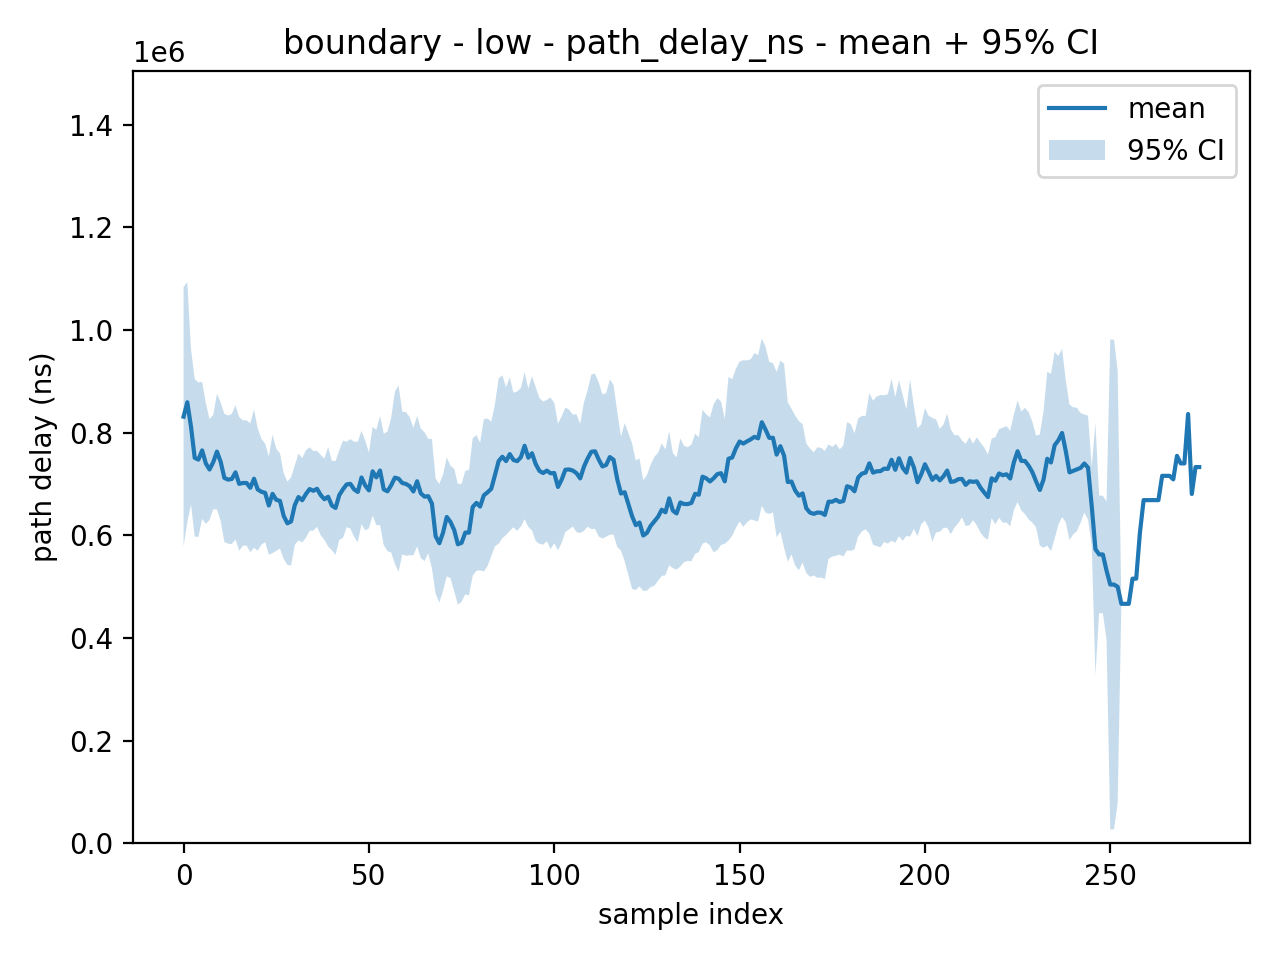
\includegraphics[width=\linewidth]{
      pars_plots/ptp/_aggregated/boundary/low/path_delay_ns_mean_ci95.png
    }
    \caption{Scenario LOW}
  \end{subfigure}
  \hfill
  \begin{subfigure}
    {0.32\textwidth}
    \centering
    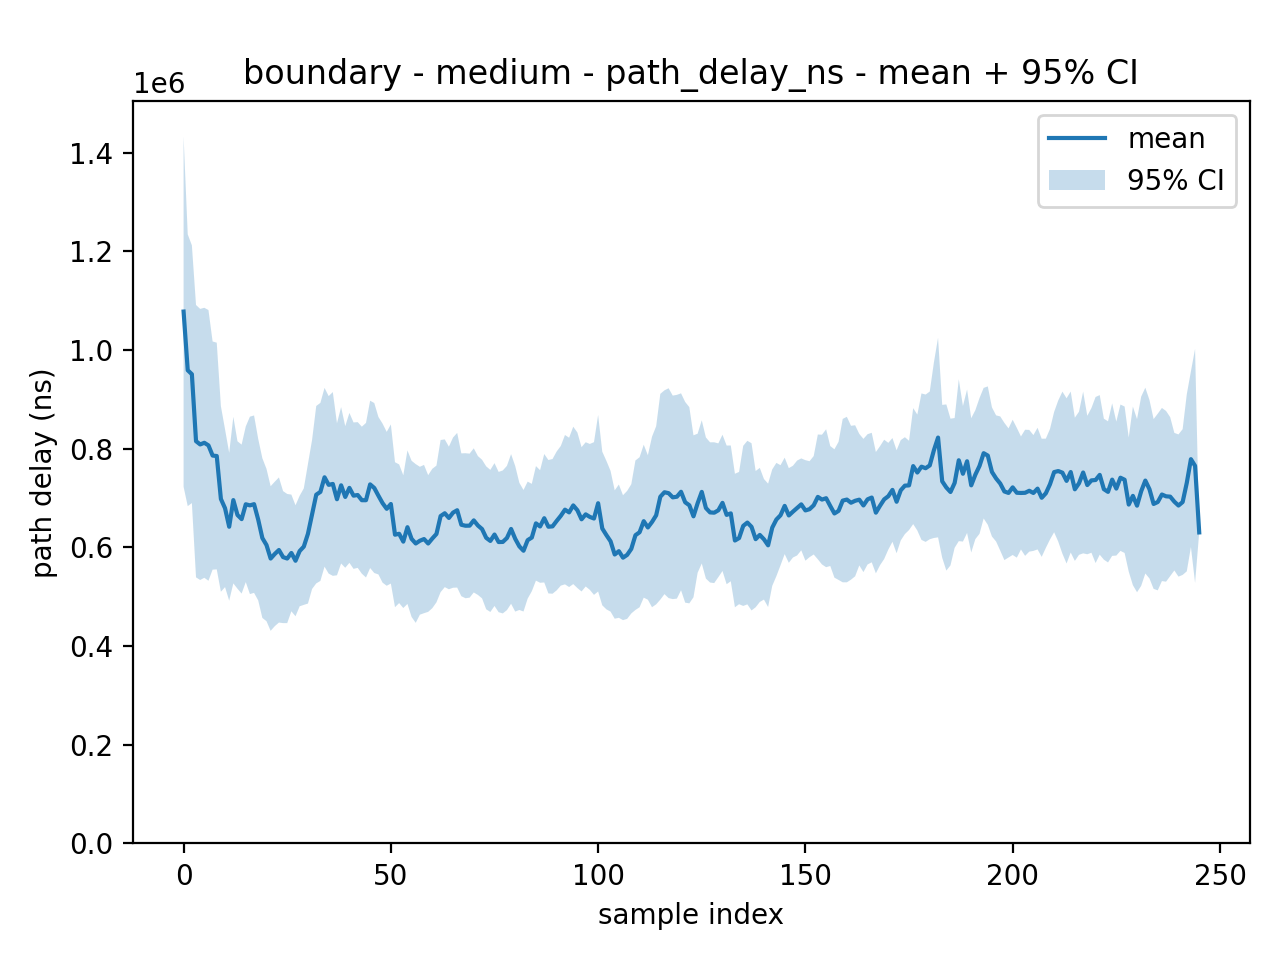
\includegraphics[width=\linewidth]{
      pars_plots/ptp/_aggregated/boundary/medium/path_delay_ns_mean_ci95.png
    }
    \caption{Scenario MEDIUM}
  \end{subfigure}
  \begin{subfigure}
    {0.32\textwidth}
    \centering
    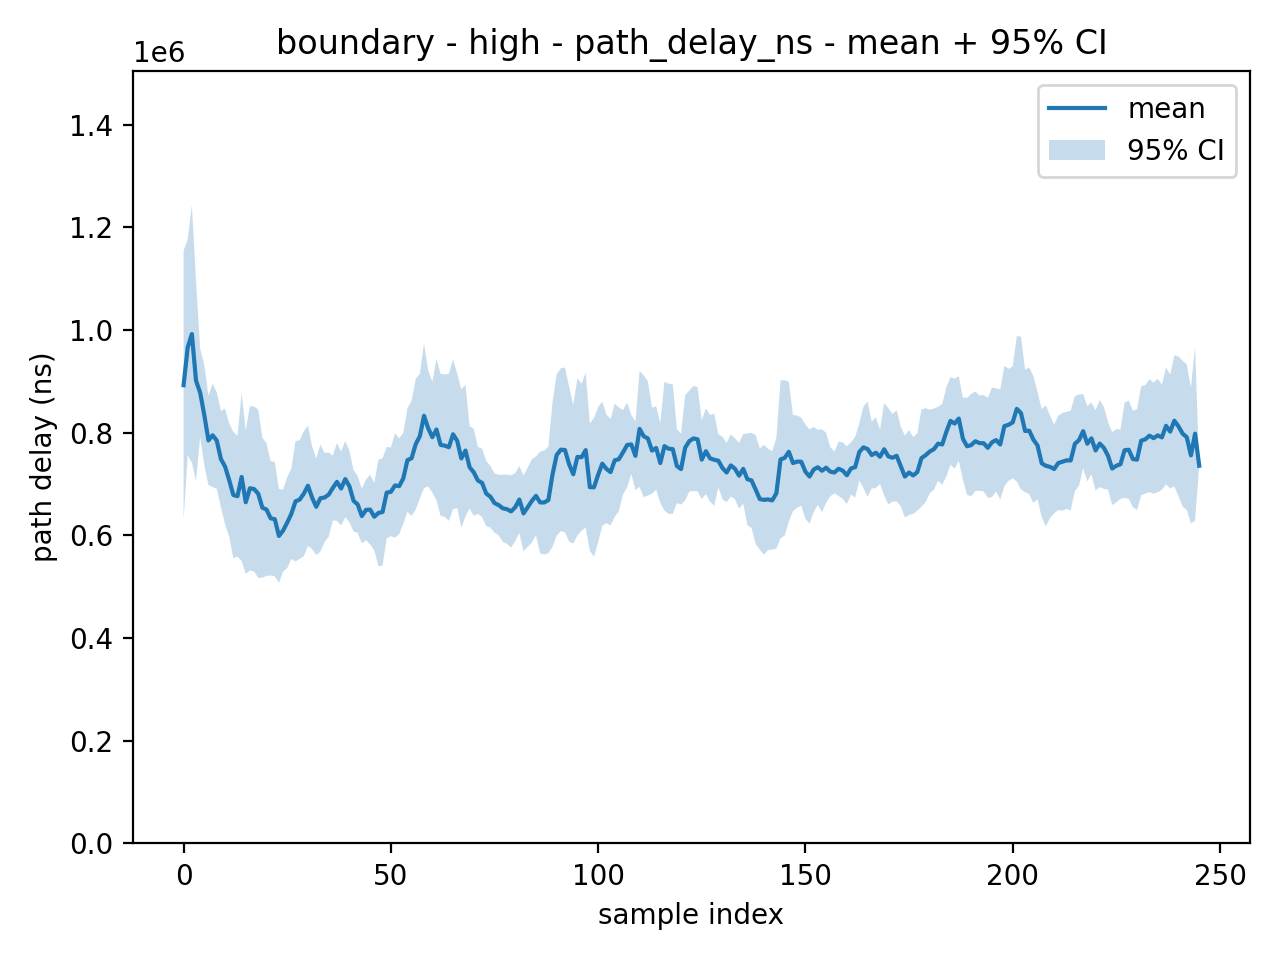
\includegraphics[width=\linewidth]{
      pars_plots/ptp/_aggregated/boundary/high/path_delay_ns_mean_ci95.png
    }
    \caption{Scenario HIGH}
  \end{subfigure}
  \caption{Media con intervallo di confidenza al 95\% - nodo: \texttt{boundary}}
  \label{fig:scenario_comparison}
\end{figure}
\begin{figure}[H]
  \centering

  \begin{subfigure}
    {0.32\textwidth}
    \centering
    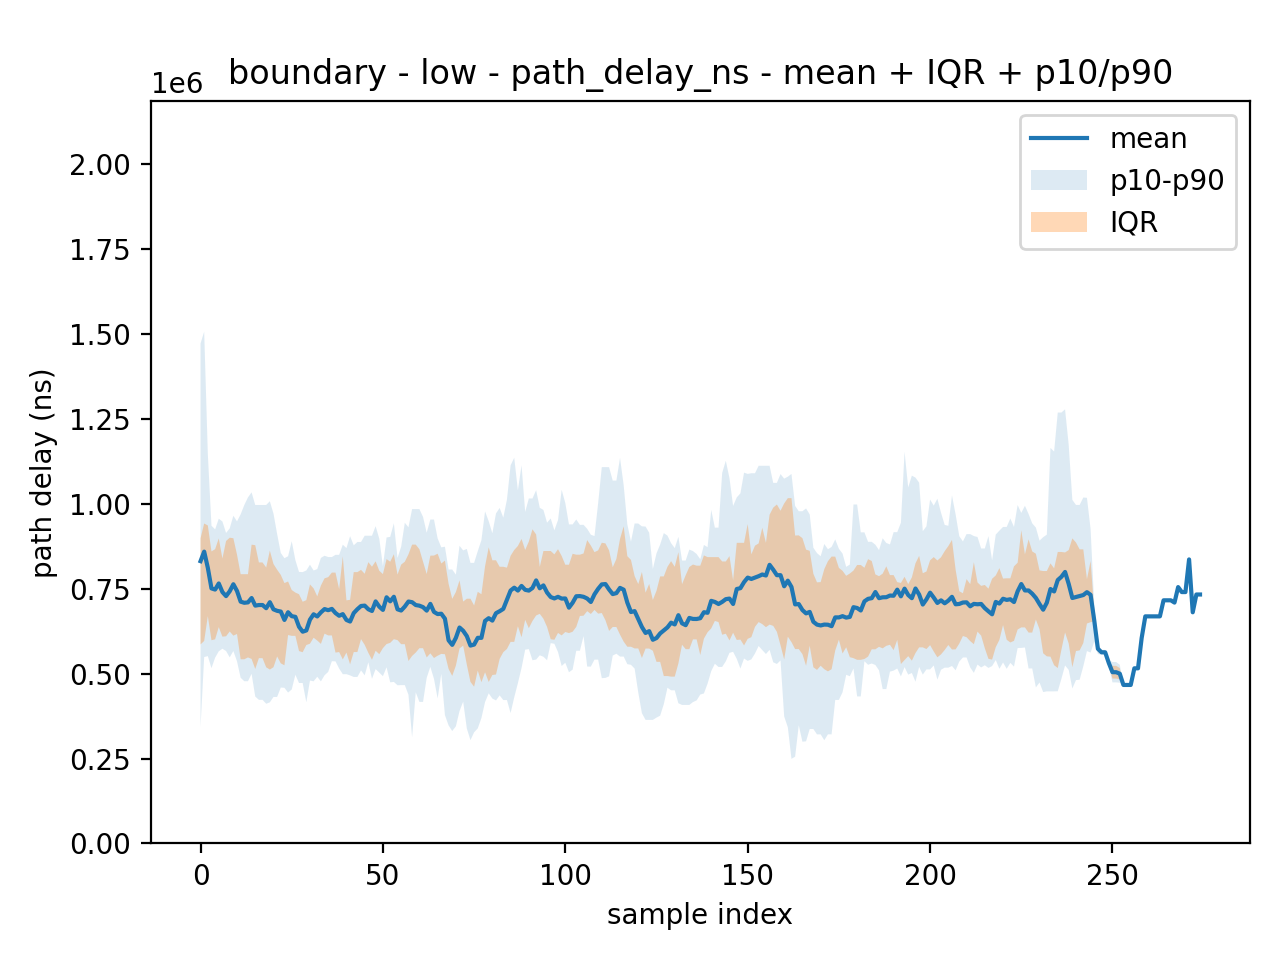
\includegraphics[width=\linewidth]{
      pars_plots/ptp/_aggregated/boundary/low/path_delay_ns_mean_iqr_p10_p90.png
    }
    \caption{Scenario LOW}
  \end{subfigure}
  \hfill
  \begin{subfigure}
    {0.32\textwidth}
    \centering
    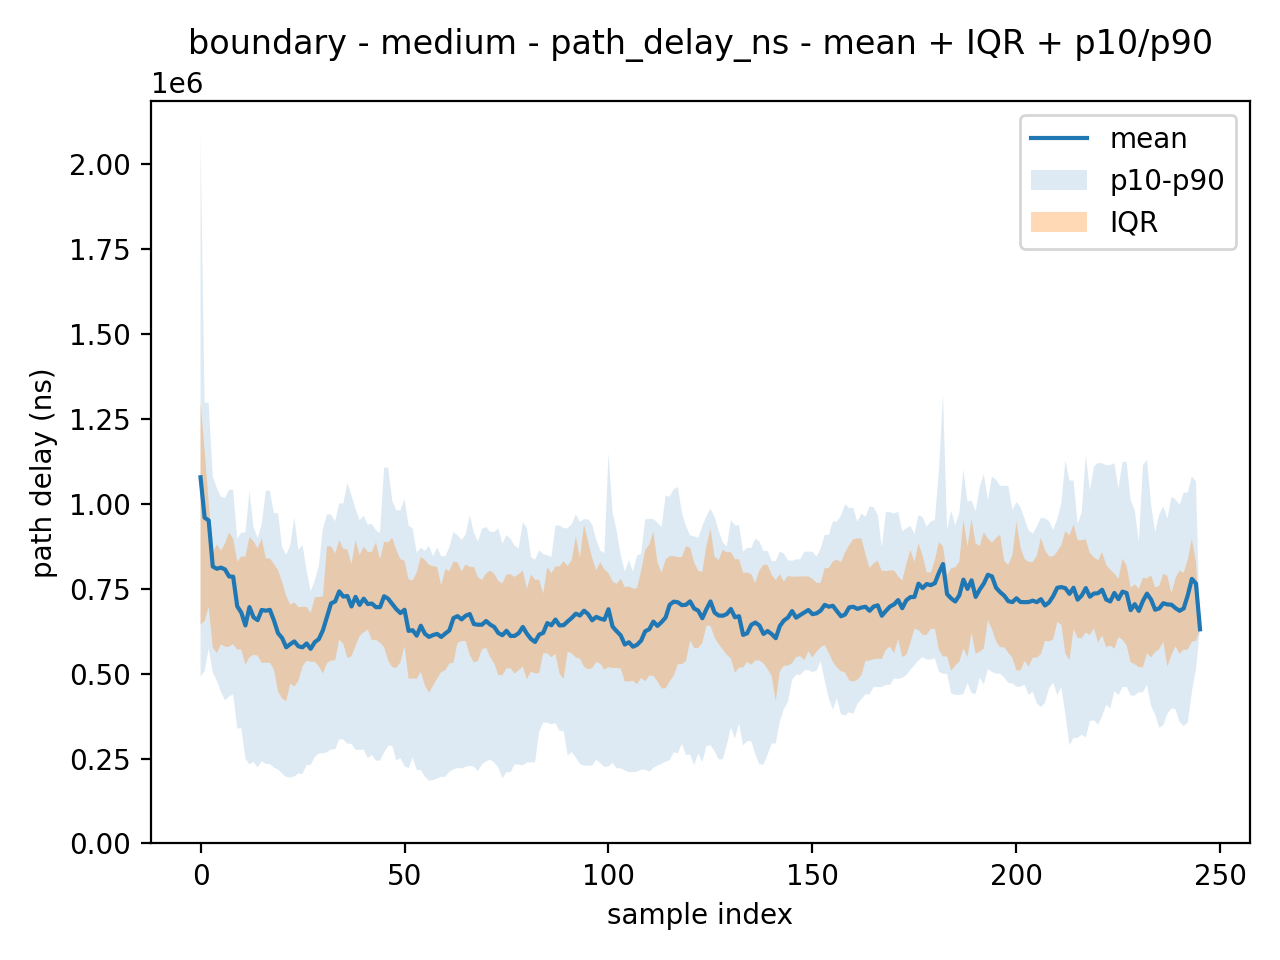
\includegraphics[width=\linewidth]{
      pars_plots/ptp/_aggregated/boundary/medium/path_delay_ns_mean_iqr_p10_p90.png
    }
    \caption{Scenario MEDIUM}
  \end{subfigure}
  \begin{subfigure}
    {0.32\textwidth}
    \centering
    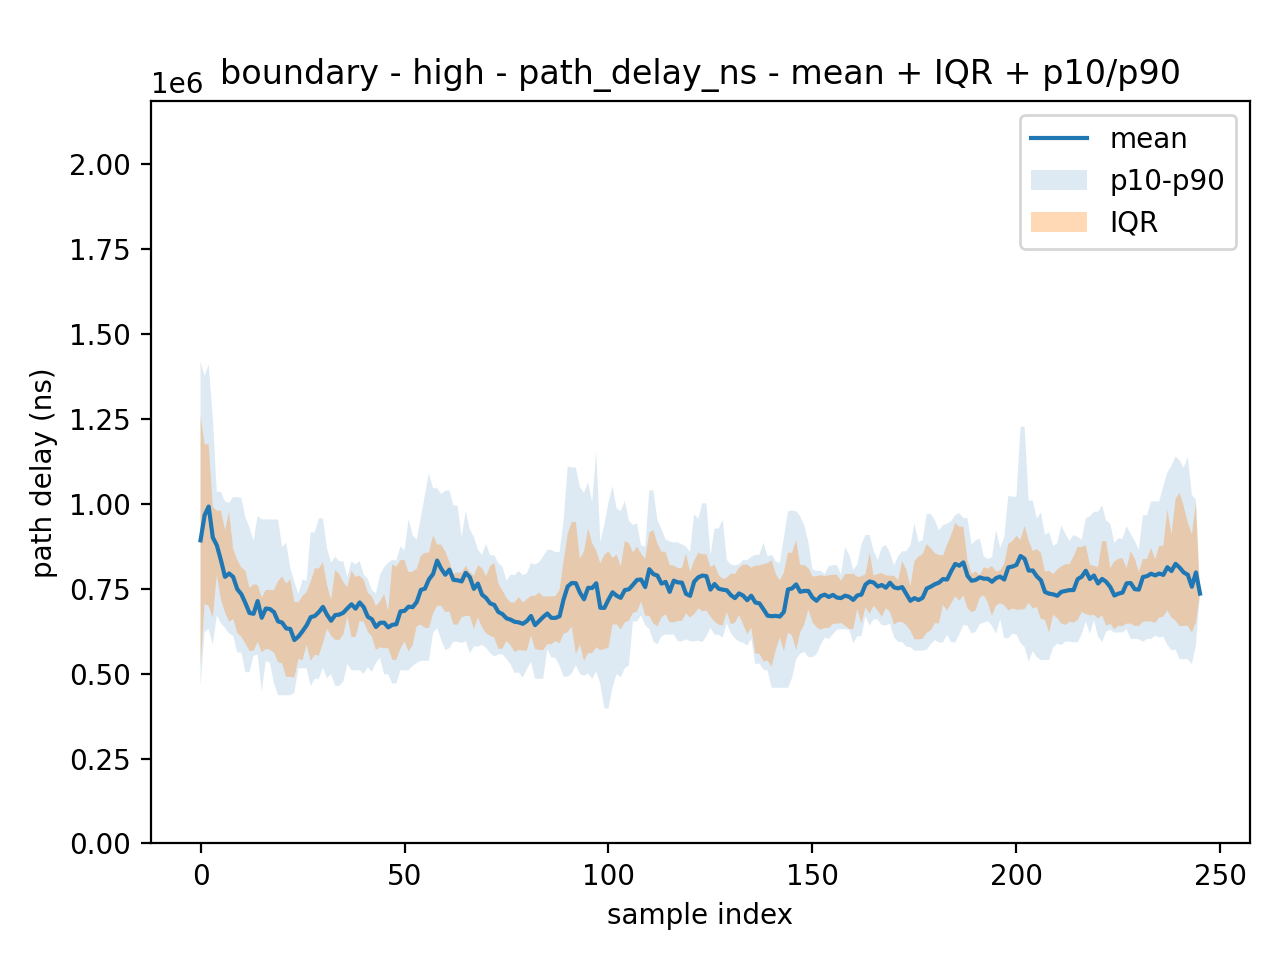
\includegraphics[width=\linewidth]{
      pars_plots/ptp/_aggregated/boundary/high/path_delay_ns_mean_iqr_p10_p90.png
    }
    \caption{Scenario HIGH}
  \end{subfigure}
  \caption{Media con banda inter-quartile e banda p10-p90 - nodo: \texttt{boundary}}
  \label{fig:scenario_comparison}
\end{figure}
Per quanto riguarda il \texttt{path delay} vi è conferma, nel complesso, dell'ipotesi.
Le tre condizioni sperimentali presentano infatti valori medi dello stesso ordine
di grandezza e profili temporali complessivamente regolari, senza evidenza di un
deterioramento sistematico e monotono.

Da un punto di vista quantitativo, si ha un valore medio aggregato del \texttt{path
delay} di ~697.227~\textmu s nello scenario \texttt{low}, 687.669~\textmu s nello
scenario \texttt{medium} e 740.415~\textmu s nello scenario \texttt{high}.
Differenze contenute nei tre casi, non indicano quindi una variazione sostanziale.
L'ampiezza inter-quartile media e la banda p10--p90 non mostrano infatti un incremento
progressivo e coerente con il livello di stress applicato.

Il grafico suggerisce, nello scenario \texttt{low} una curva media attorno a un stabile,
con eventuali fluttuazioni locali. Lo scenario \texttt{medium} mostra un
andamento particolarmente regolare nel tratto centrale, mentre nello scenario \texttt{high}
si osserva un innalzamento moderato del livello medio, comunque compatibile con una
condizione di sincronizzazione ancora stabile.

Per quanto riguarda la metrica del \texttt{path delay} c'è conferma sperimentale
dell'assenza di degrado strutturato. Le variazioni osservate possono essere interpretate
più plausibilmente come effetti indiretti del funzionamento complessivo del demone
\texttt{ptp4l}.

\subsubsection{Analisi metrica: \texttt{offset}}
\begin{figure}[H]
  \centering

  \begin{subfigure}
    {0.32\textwidth}
    \centering
    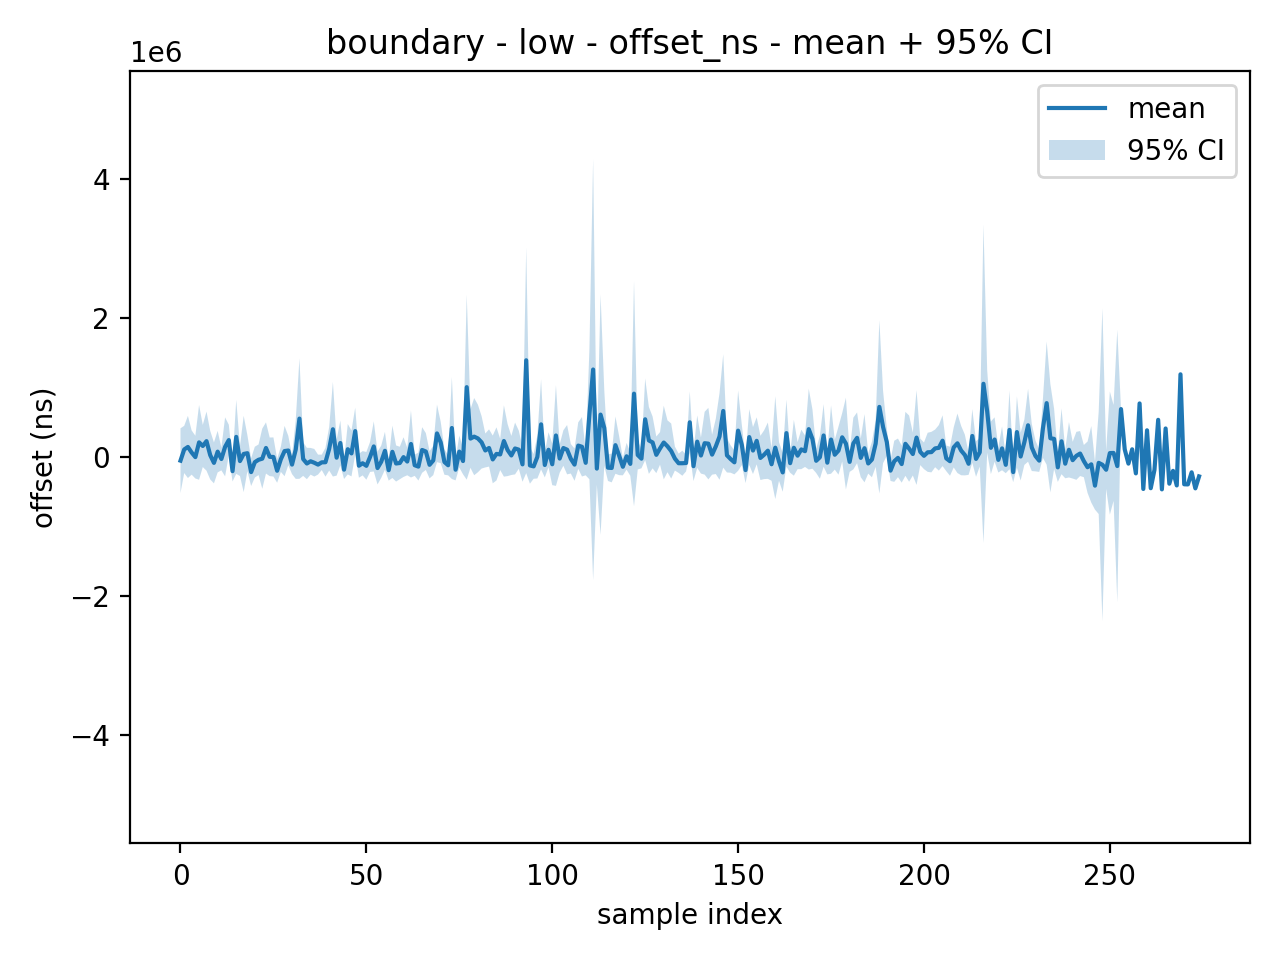
\includegraphics[width=\linewidth]{
      pars_plots/ptp/_aggregated/boundary/low/offset_ns_mean_ci95.png
    }
    \caption{Scenario LOW}
  \end{subfigure}
  \hfill
  \begin{subfigure}
    {0.32\textwidth}
    \centering
    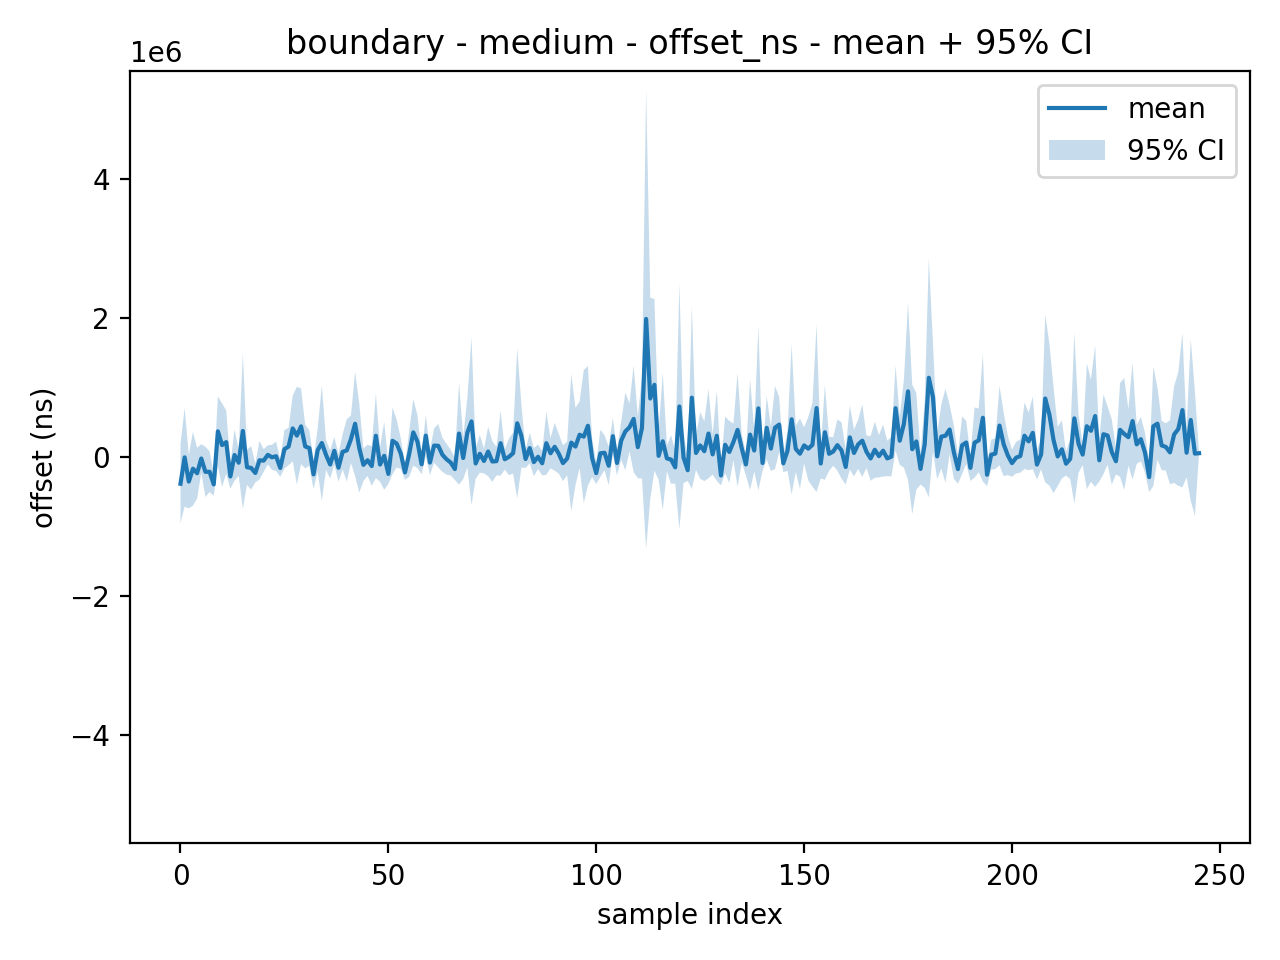
\includegraphics[width=\linewidth]{
      pars_plots/ptp/_aggregated/boundary/medium/offset_ns_mean_ci95.png
    }
    \caption{Scenario MEDIUM}
  \end{subfigure}
  \begin{subfigure}
    {0.32\textwidth}
    \centering
    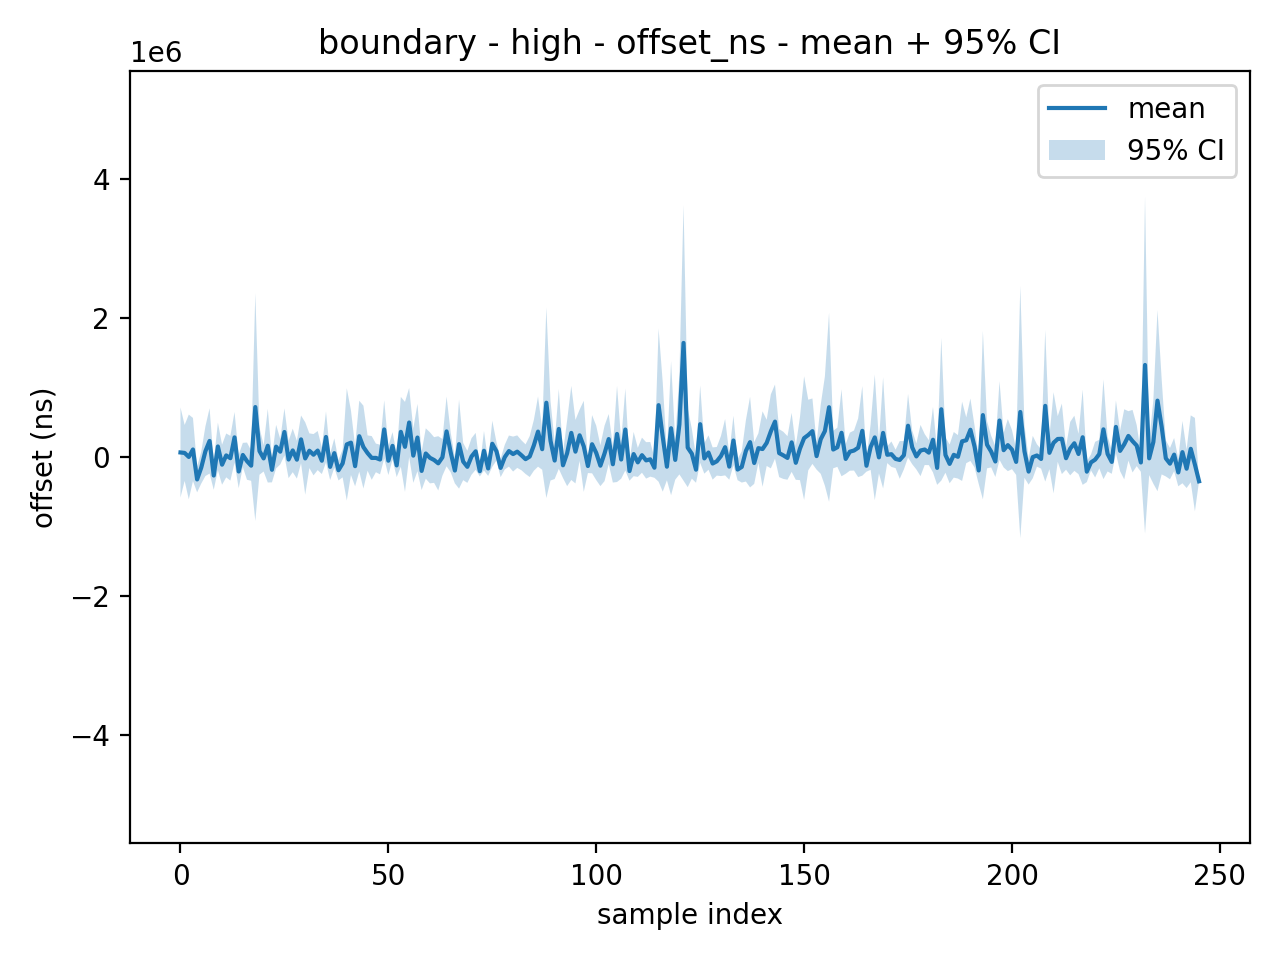
\includegraphics[width=\linewidth]{
      pars_plots/ptp/_aggregated/boundary/high/offset_ns_mean_ci95.png
    }
    \caption{Scenario HIGH}
  \end{subfigure}
  \caption{Media con intervallo di confidenza al 95\% - nodo: \texttt{boundary} -
  dati completi}
  \label{fig:scenario_comparison}
\end{figure}
\begin{figure}[H]
  \centering

  \begin{subfigure}
    {0.32\textwidth}
    \centering
    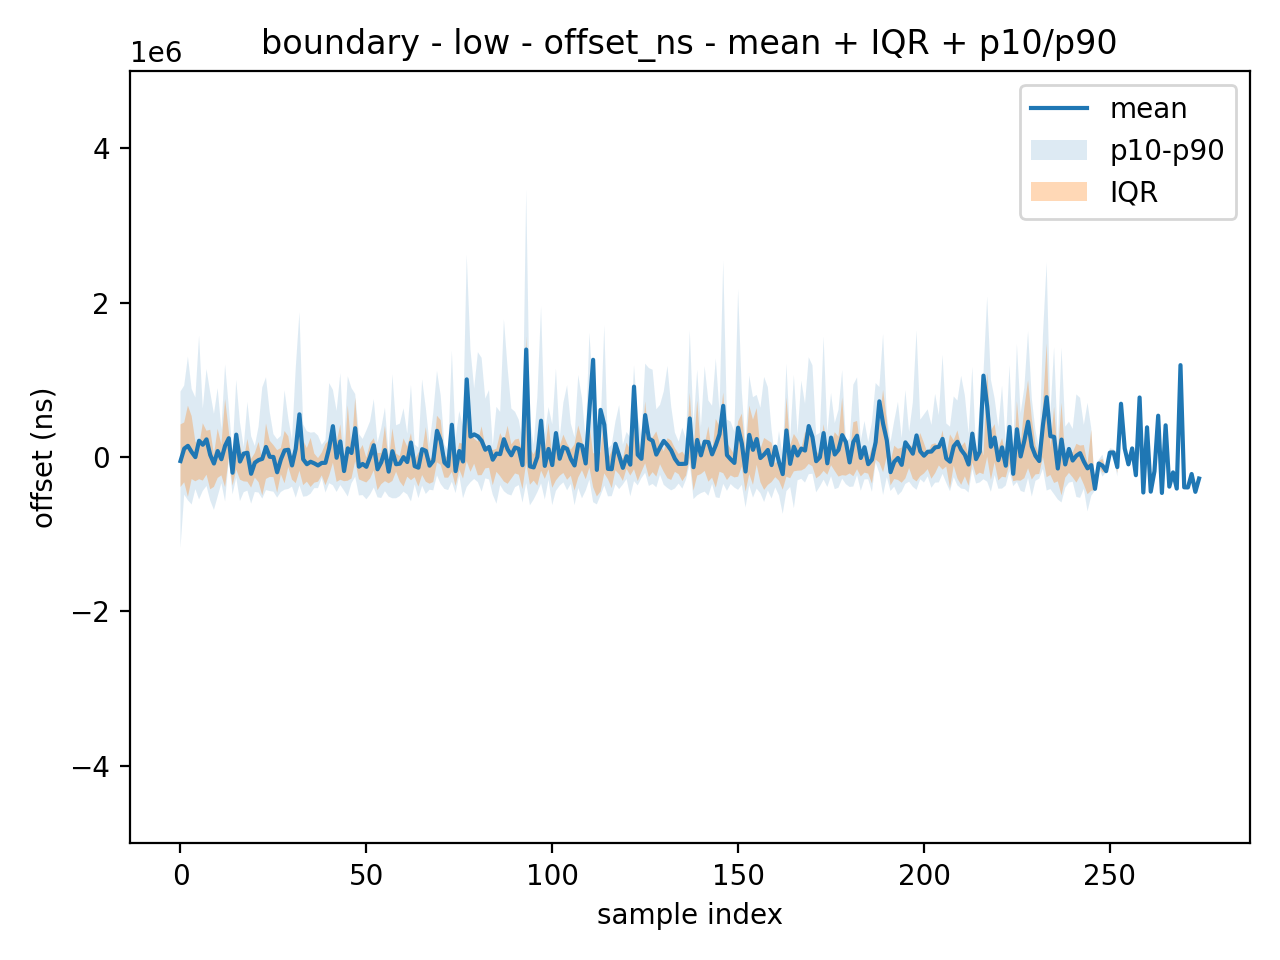
\includegraphics[width=\linewidth]{
      pars_plots/ptp/_aggregated/boundary/low/offset_ns_mean_iqr_p10_p90.png
    }
    \caption{Scenario LOW}
  \end{subfigure}
  \hfill
  \begin{subfigure}
    {0.32\textwidth}
    \centering
    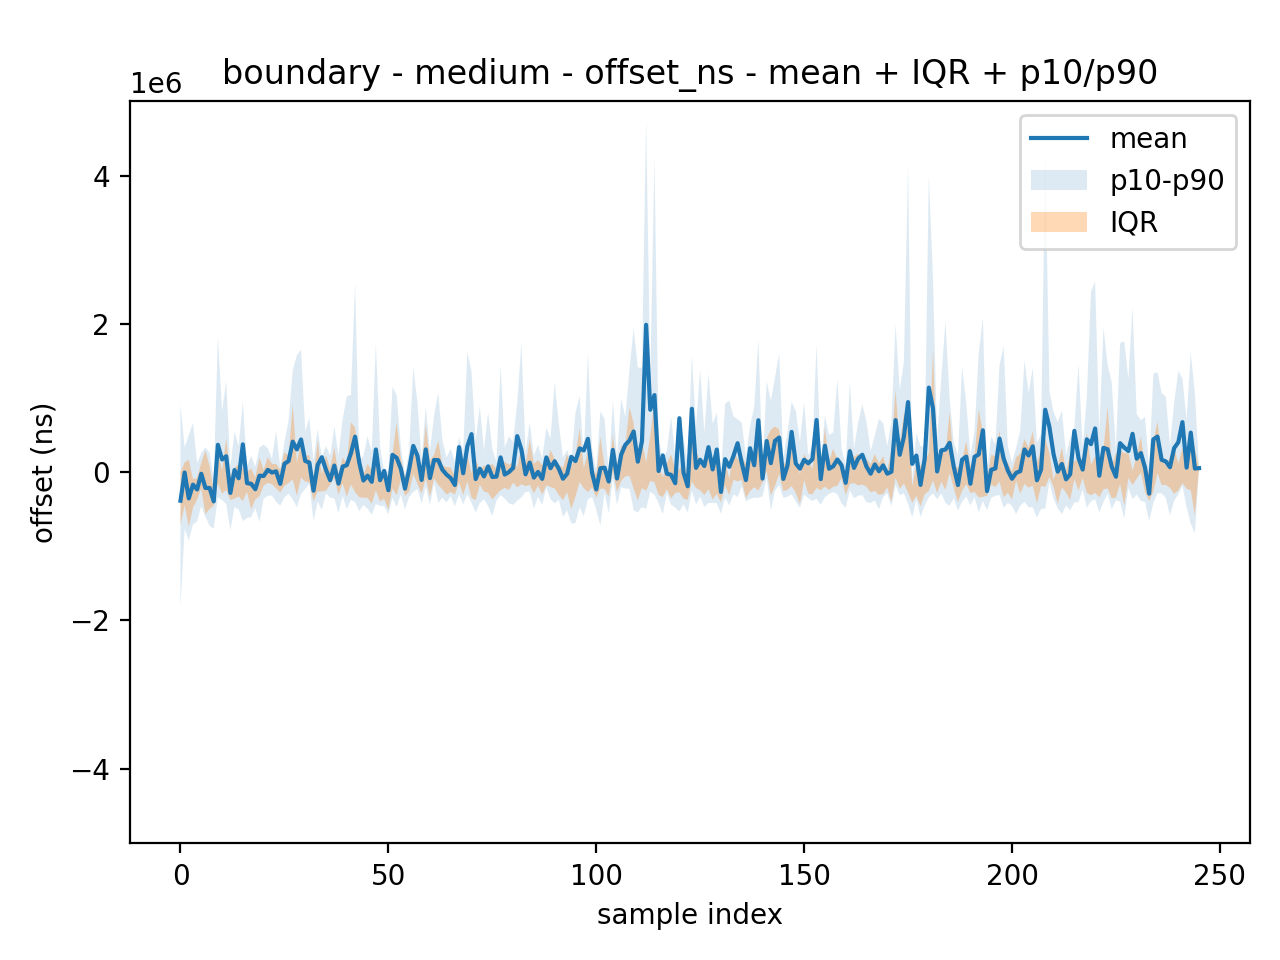
\includegraphics[width=\linewidth]{
      pars_plots/ptp/_aggregated/boundary/medium/offset_ns_mean_iqr_p10_p90.png
    }
    \caption{Scenario MEDIUM}
  \end{subfigure}
  \begin{subfigure}
    {0.32\textwidth}
    \centering
    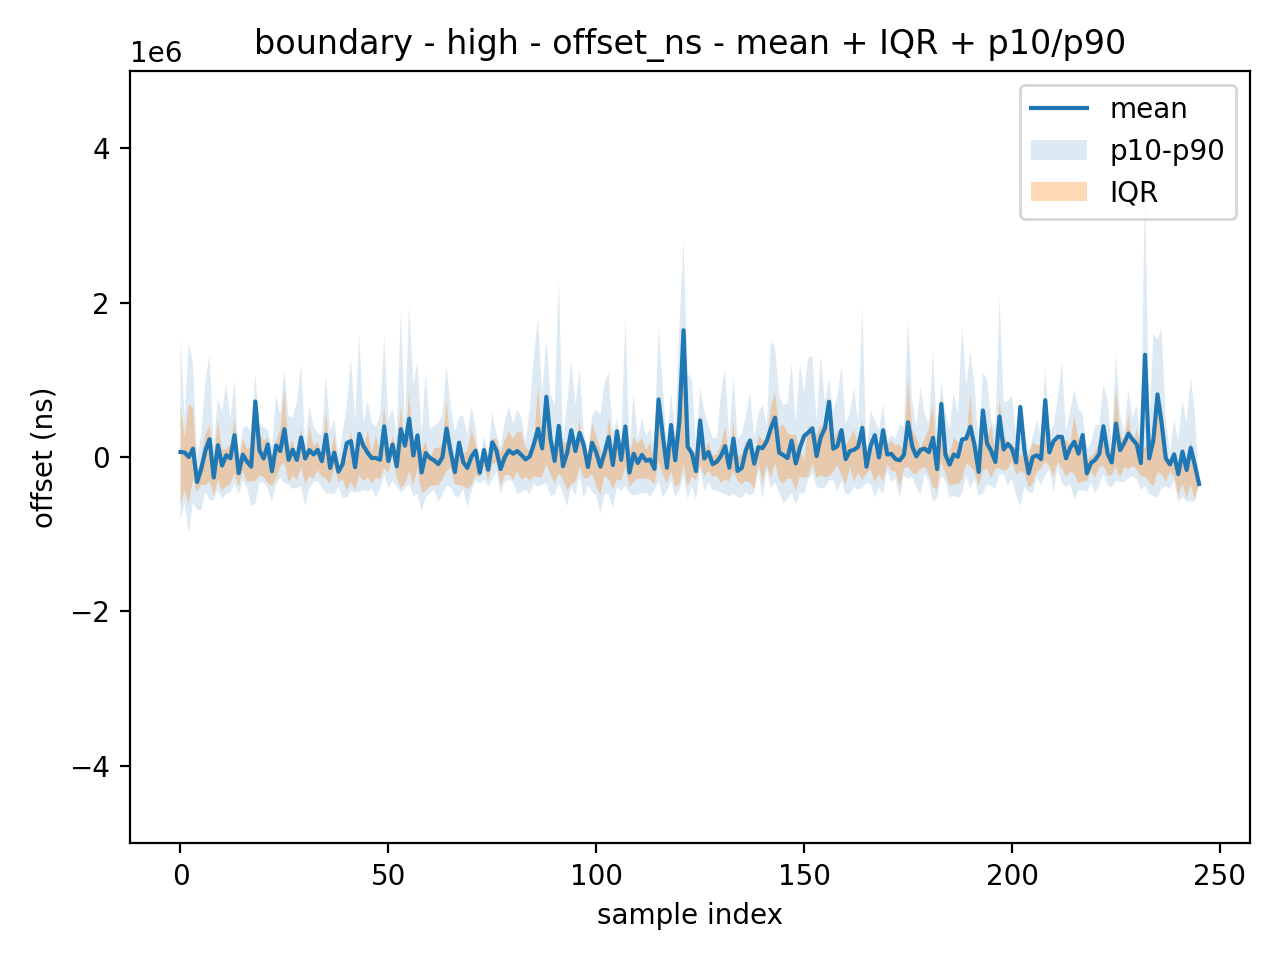
\includegraphics[width=\linewidth]{
      pars_plots/ptp/_aggregated/boundary/high/offset_ns_mean_iqr_p10_p90.png
    }
    \caption{Scenario HIGH}
  \end{subfigure}
  \caption{Media con banda inter-quartile e banda p10-p90 - nodo: \texttt{boundary}}
  \label{fig:scenario_comparison}
\end{figure}

Anche i dati dell'\texttt{offset} confermano il trend. I tre scenari evidenziano un
andamento complessivamente centrato in prossimità dello zero, con oscillazioni
di segno alterno e picchi sporadici.

Il valore medio dell'\texttt{offset} è di ~87.809~\textmu s nello scenario
\texttt{low}, ~153.961~\textmu s nello scenario \texttt{medium} e ~110.782~\textmu
s nello scenario \texttt{high}. La mediana assume valori contenuti rispettivamente
nei tre scenari,con valori di ~45.375~\textmu s, ~97.301~\textmu s e ~65.087~\textmu
s. I risultati mostrano una lieve prevalenza di offset positivo, ma sempre compatibile
con le premesse.

L'ampiezza inter-quartile media è di ~279.114~\textmu s nello scenario \texttt{low},
~327.530~\textmu s nello scenario \texttt{medium} e ~250.843~\textmu s nello scenario
\texttt{high}. La banda p10--p90 media assume valori pari a circa 1017.673~\textmu
s, 1243.040~\textmu s e 1122.148~\textmu s. L'osservazione dei profili temporali
porta alle stesse conclusioni.

Nel complesso, l'\texttt{offset} del \texttt{boundary} conferma una condizione di
stabilità della sincronizzazione. Le differenze osservate tra i tre scenari
appaiono limitate, non monotone e non sufficienti a sostenere l'ipotesi di un impatto
diretto del degrado downstream sulla sincronizzazione del \texttt{boundary}
rispetto al \texttt{servergm}.

\section{\texttt{chronyd}}
Per quanto riguarda il demone \texttt{Chrony}, l'analisi è stata svolta su una topologia
composta dal solo collegamento tra \texttt{servergm} e \texttt{clientchrony}. In
questo contesto, il degrado di rete tramite \texttt{tc}/\texttt{netem} è stato applicato
in due configurazioni distinte: in un primo caso sull'interfaccia del \texttt{clientchrony},
in un secondo caso sull'interfaccia del \texttt{servergm}.

La doppia configurazione permette di osservare in modo separato effetti del degrado
introdotto lungo le due direzioni logiche della comunicazione tra client e server.

Nei risultati proposti, quindi, oltre alla comparazione dei differenti scenari,
si ha la distinzione delle due configurazioni.È utile precisare che tutte le
metriche analizzate sono state rilevate esclusivamente tramite interrogazione
del nodo \texttt{clientchrony}, poiché è da esso che si ricavano le misure
direttamente rilevanti per valutare la qualità della sincronizzazione dal punto
di vista del client.

\subsection{Analisi metrica: \texttt{offset}}
\begin{figure}[H]
  \centering

  \begin{subfigure}
    {0.32\textwidth}
    \centering
    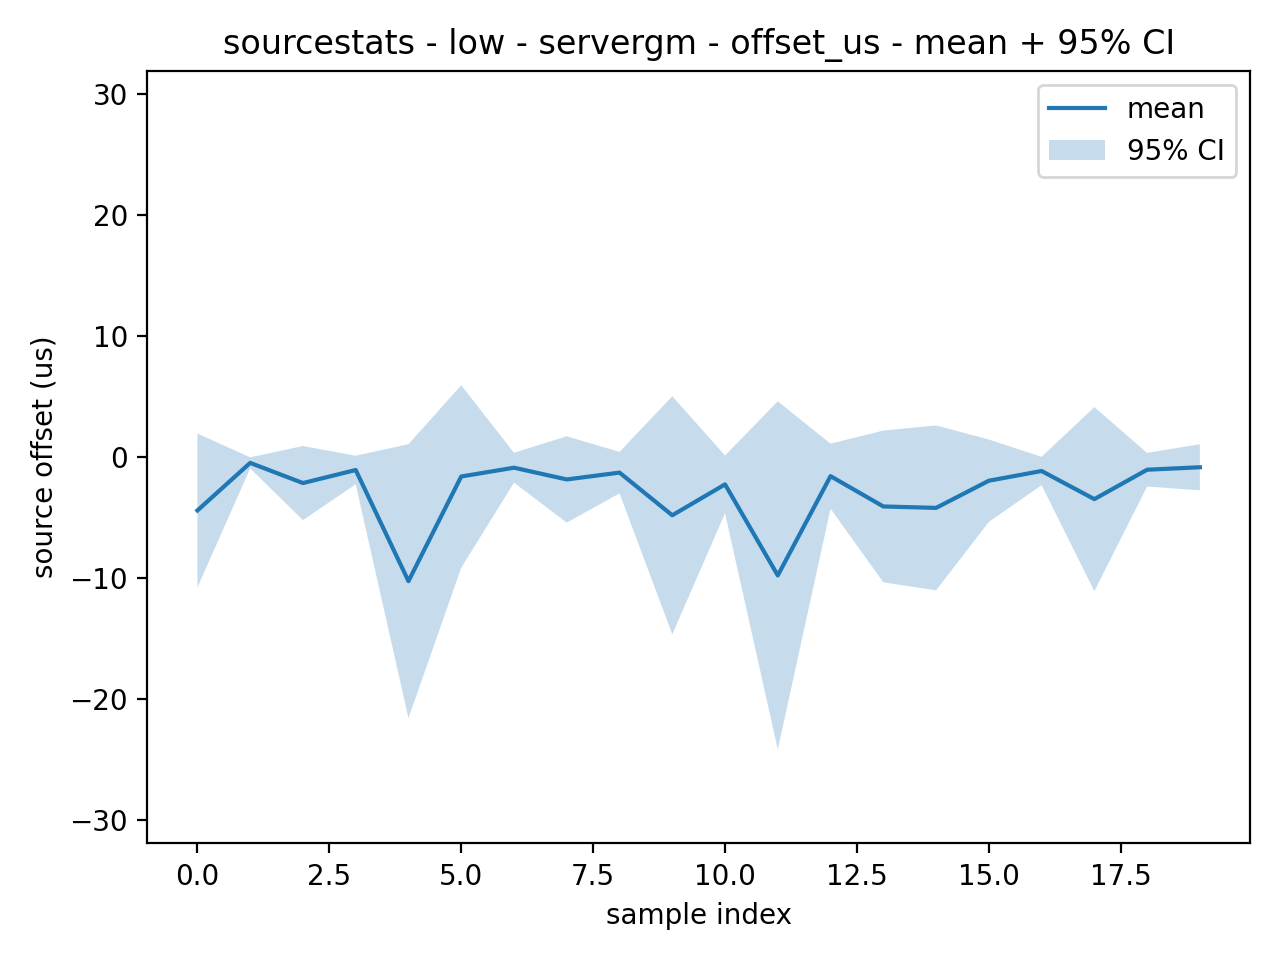
\includegraphics[width=\linewidth]{
      pars_plots/chrony_clientchrony/_aggregated/sourcestats/low/servergm/offset_us_mean_ci95.png
    }
    \caption{Scenario LOW}
  \end{subfigure}
  \hfill
  \begin{subfigure}
    {0.32\textwidth}
    \centering
    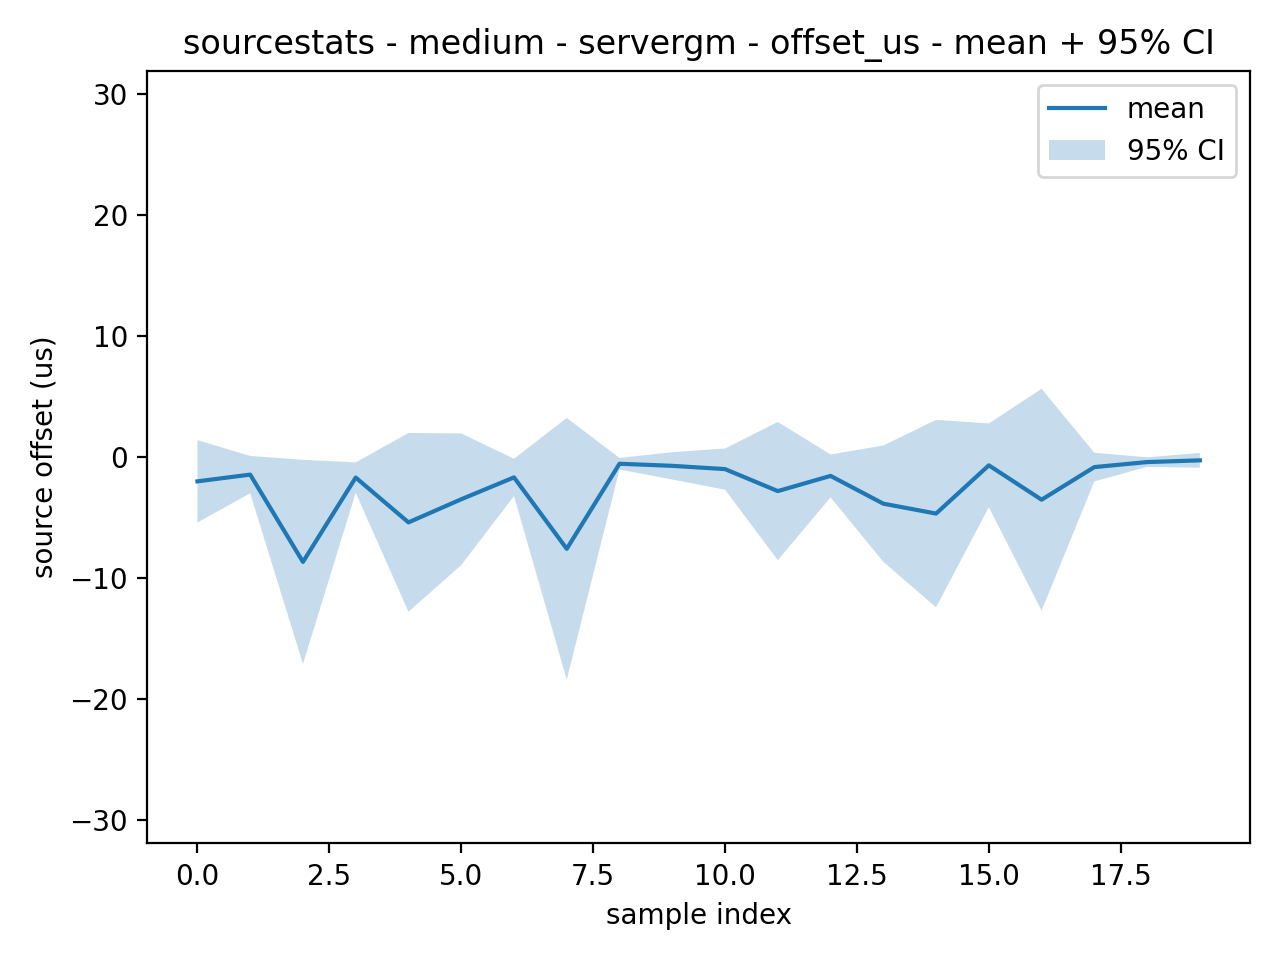
\includegraphics[width=\linewidth]{
      pars_plots/chrony_clientchrony/_aggregated/sourcestats/medium/servergm/offset_us_mean_ci95.png
    }
    \caption{Scenario MEDIUM}
  \end{subfigure}
  \begin{subfigure}
    {0.32\textwidth}
    \centering
    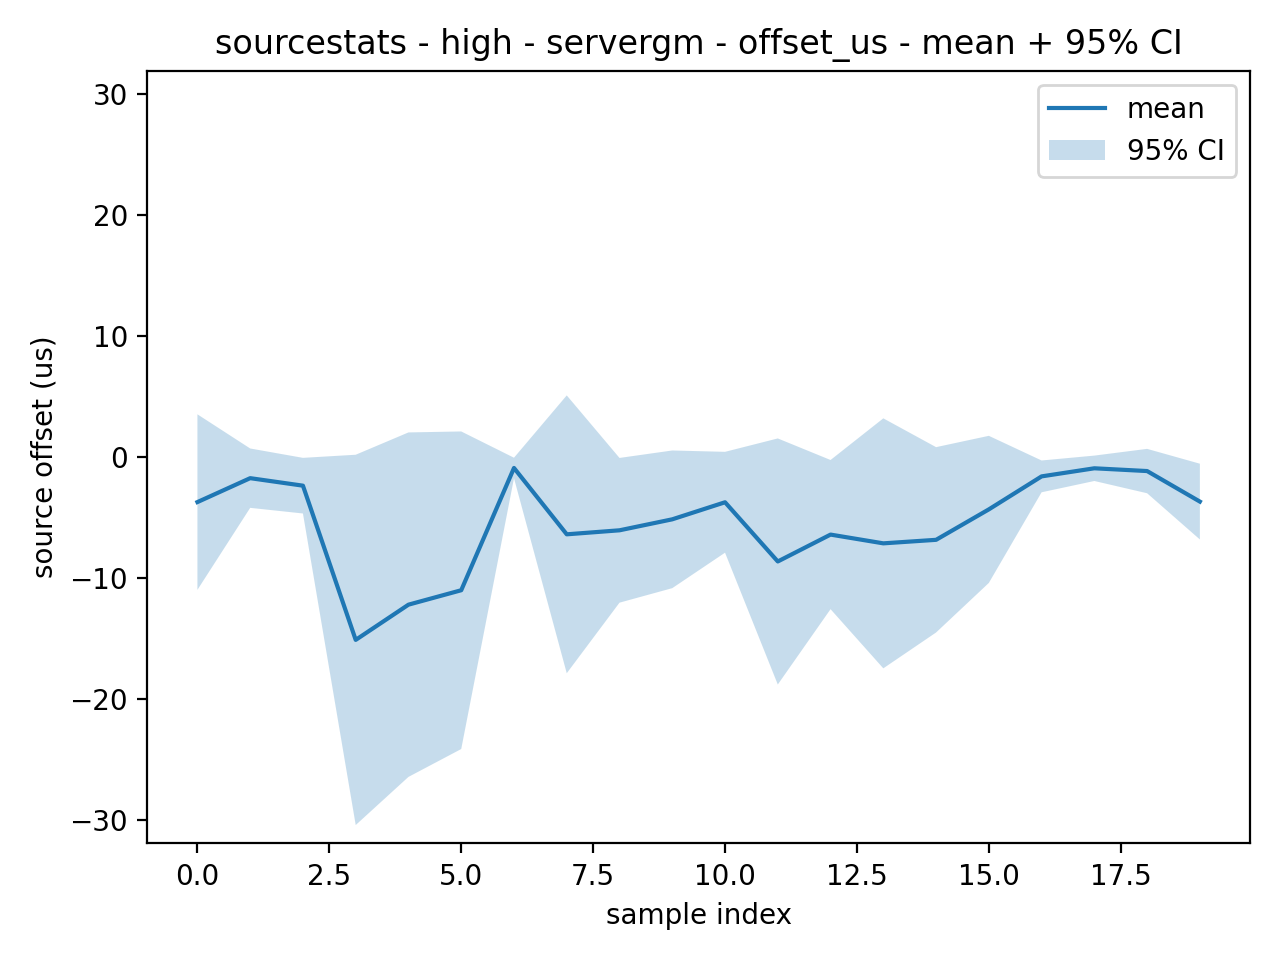
\includegraphics[width=\linewidth]{
      pars_plots/chrony_clientchrony/_aggregated/sourcestats/high/servergm/offset_us_mean_ci95.png
    }
    \caption{Scenario HIGH}
  \end{subfigure}
  \caption{Media con intervallo di confidenza al 95\% - nodo: \texttt{clientchrony}
  - netem/tc: \texttt{clientchrony}}
  \label{fig:scenario_comparison}
\end{figure}
\begin{figure}[H]
  \centering

  \begin{subfigure}
    {0.32\textwidth}
    \centering
    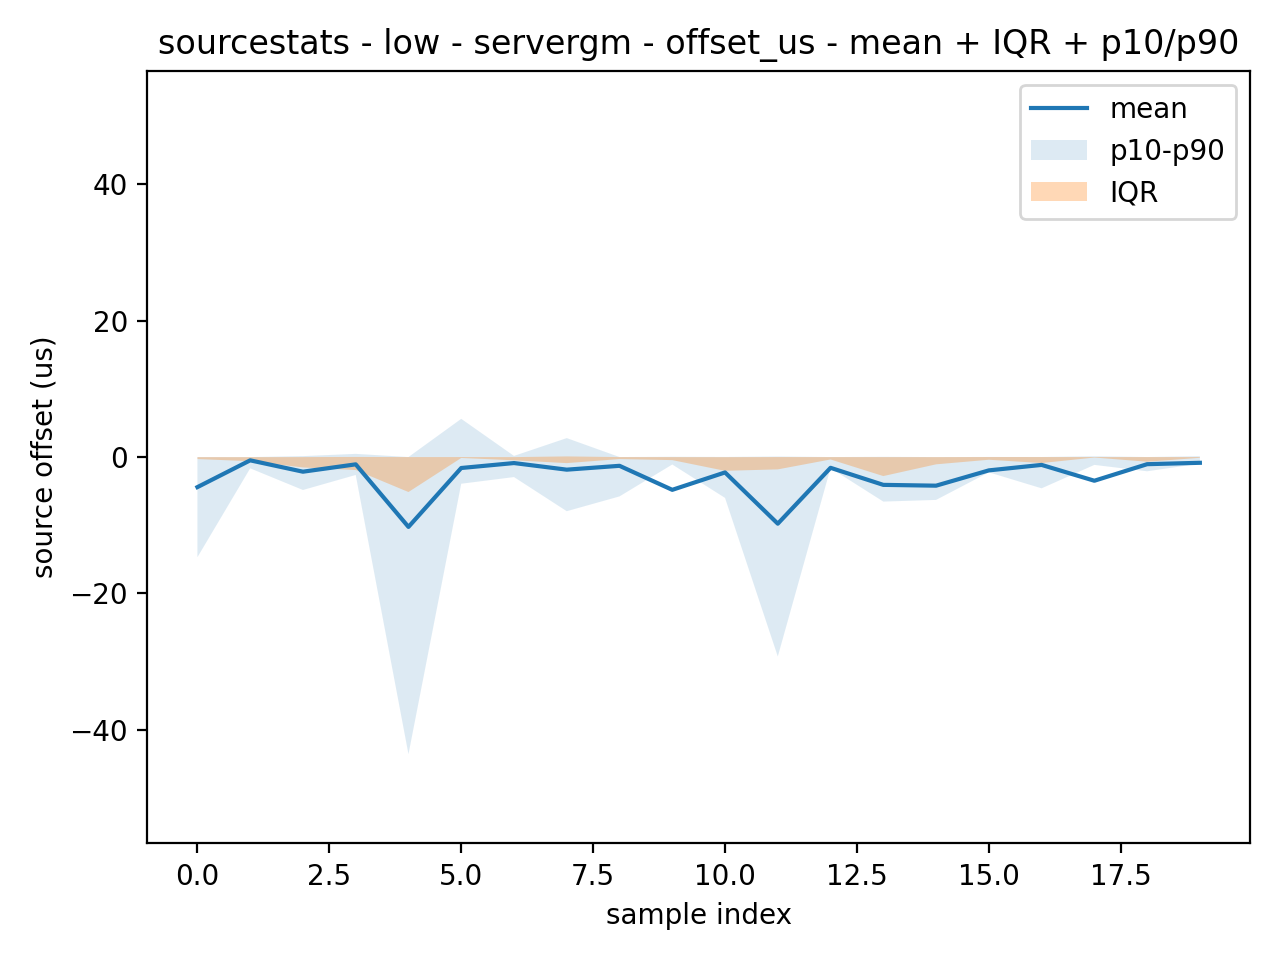
\includegraphics[width=\linewidth]{
      pars_plots/chrony_clientchrony/_aggregated/sourcestats/low/servergm/offset_us_mean_iqr_p10_p90.png
    }
    \caption{Scenario LOW}
  \end{subfigure}
  \hfill
  \begin{subfigure}
    {0.32\textwidth}
    \centering
    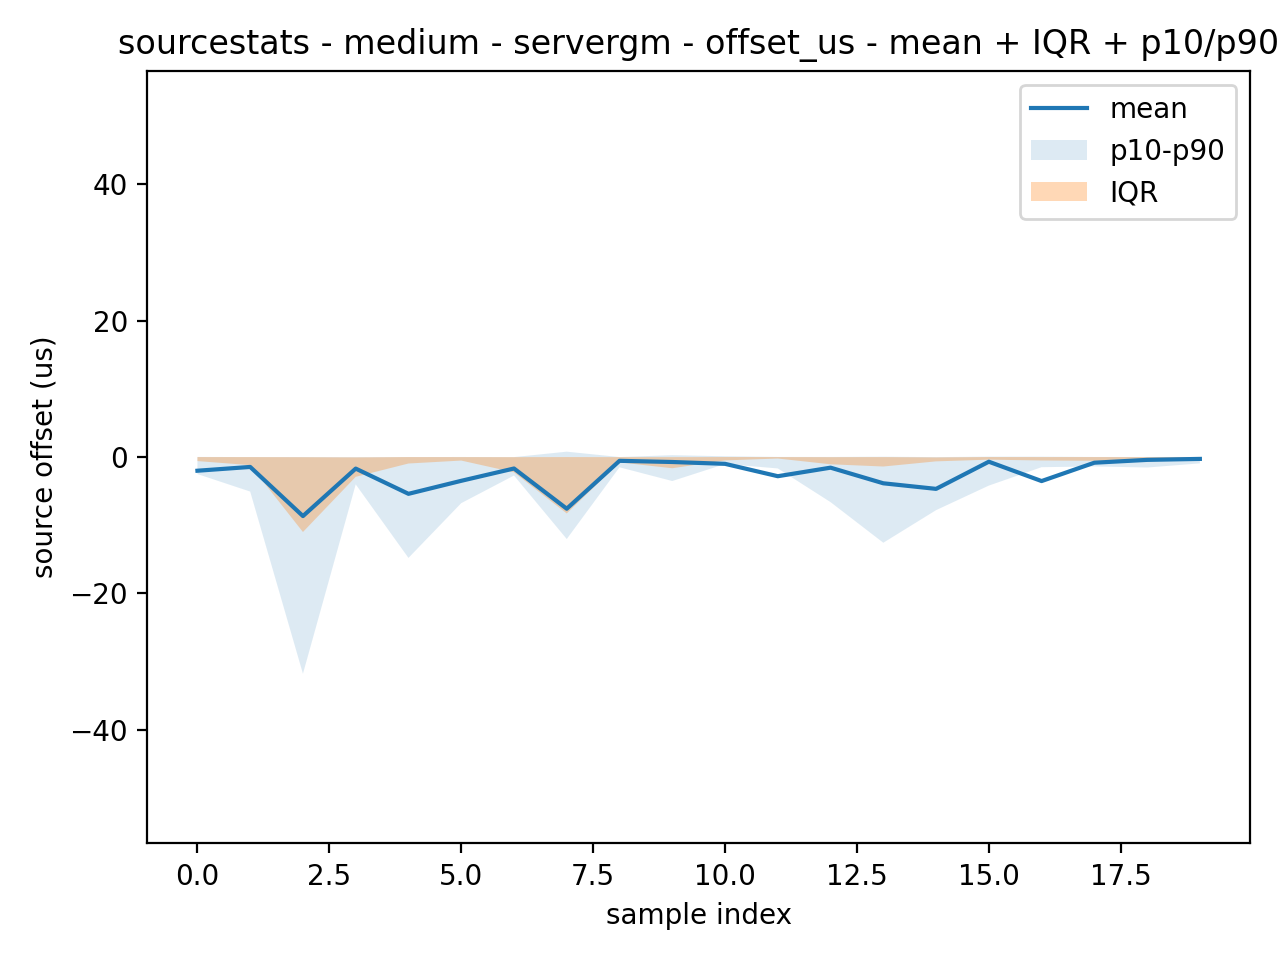
\includegraphics[width=\linewidth]{
      pars_plots/chrony_clientchrony/_aggregated/sourcestats/medium/servergm/offset_us_mean_iqr_p10_p90.png
    }
    \caption{Scenario MEDIUM}
  \end{subfigure}
  \begin{subfigure}
    {0.32\textwidth}
    \centering
    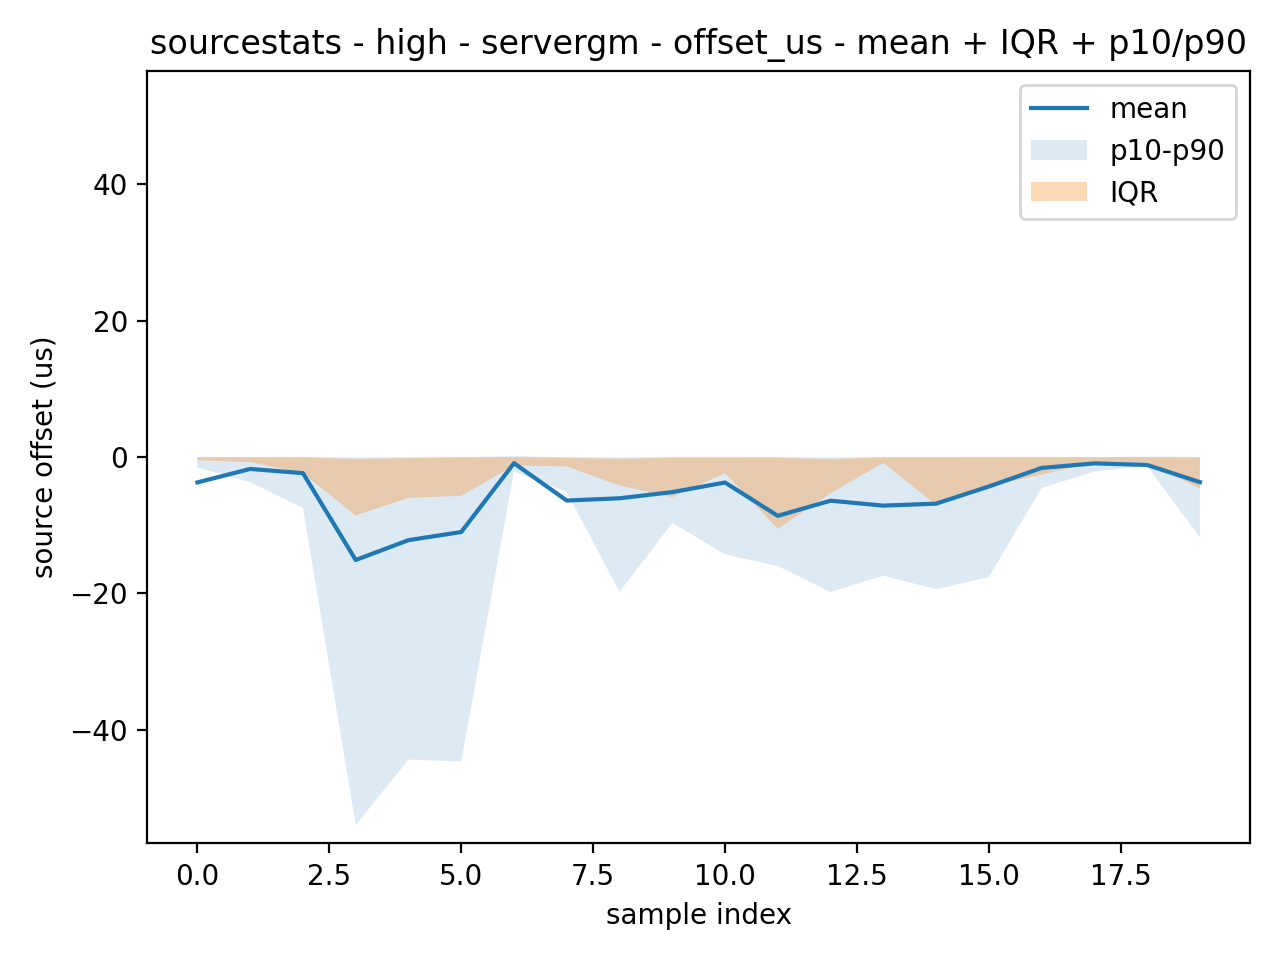
\includegraphics[width=\linewidth]{
      pars_plots/chrony_clientchrony/_aggregated/sourcestats/high/servergm/offset_us_mean_iqr_p10_p90.png
    }
    \caption{Scenario HIGH}
  \end{subfigure}
  \caption{Media con banda inter-quartile e banda p10-p90 - nodo: \texttt{clientchrony}
  - netem/tc: \texttt{clientchrony}}
  \label{fig:scenario_comparison}
\end{figure}
\paragraph*{clientchrony - netem/tc:}
Nel caso della metrica \texttt{offset\_us}, l'analisi relativa a \texttt{clientchrony}
vi è un peggioramento progressivo all'aumentare dell'intensità dello scenario, nonostante
non venga compromessa la sincronizzazione verso la sorgente.

Nel caso \texttt{low}, si ha una curva delle medie vicino all zero, ma con
prevalenza di valori leggermente negativi. L'aggregazione sulle curve fornisce una
media di ~\texttt{-2.958 \,$\mu$s} e i valori medi sono compresi nell'intervallo ~\texttt{-10.250
\,$\mu$s} e ~\texttt{-0.481 \,$\mu$s}. Per quanto riguarda le statistiche
globali sui campioni si ha la mediana pari a ~\texttt{-0.049 \,$\mu$s}, il primo quartile
è ~\texttt{-0.927 \,$\mu$s} e il terzo quartile è ~\texttt{-0.002 \,$\mu$s}. L'ampiezza
media dell'intervallo ~\texttt{p10-p90}, pari a ~\texttt{7.971 \,$\mu$s}. La
banda inter-quartile media è contenuta, con un valore di ~\texttt{1.095 \,$\mu$s}.
In questo scenario il degrado introdotto sul client produce soltanto un lieve
sbilanciamento negativo dell'offset, senza alterare in modo significativo il regime
di sincronizzazione.

Nel caso \texttt{medium} cresce la dispersione e compaiono fluttuazioni negative
più frequenti. La media della curva aggregata è pari a \texttt{-2.642 \,$\mu$s}, simile
al caso \texttt{low}, ma i grafici evidenziano dei picchi più accentuati. La
mediana è ~\texttt{-0.073 \,$\mu$s}, il primo quartile ~\texttt{-1.075 \,$\mu$s} e
il terzo quartile ~\texttt{-0.004 \,$\mu$s}. Il peggioramento è principalmente
evidente nella variabilità. L'ampiezza media della banda \texttt{p10-p90} è di ~\texttt{6.266
\,$\mu$s}. La banda inter-quartile media cresce a \texttt{1.804 \,$\mu$s}.Inoltre,
il valore massimo dell'IQR raggiunge \texttt{10.978 \,$\mu$s}, segnale che in
alcuni punti il comportamento tra le run diventa più irregolare.

Nello scenario \texttt{high}, la media delle curve aggregate scende a \texttt{-5.451
\,$\mu$s}, quindi circa il doppio in valore assoluto rispetto ai casi \texttt{low}
e \texttt{medium}, e la curva delle medie mostra tratti più chiaramente distanti dallo
zero, con minimi fino a \texttt{-15.103 \,$\mu$s}. La mediana resta vicino allo
zero (\texttt{-0.360 \,$\mu$s}). Non c'è quindi un peggioramento uniforme su
tutti i campioni. Vi è un aumento della dispersione. L'ampiezza media dell'intervallo
\texttt{p10-p90} è di ~\texttt{15.836 \,$\mu$s}, e l'IQR medio è di ~\texttt{3.693
\,$\mu$s}.

In tutti e tre gli scenari, in molteplici punti, la curva media è esterna alla banda inter-quartile.
Quindi si ha un valore medio non coincidente con il comportamento tipico della run, risentendo maggiormente
di anomalie o di code negative della distribuzione.

Nei primi due casi i risultati sono sufficientemente uniformi, mentre nello scenario
\texttt{high} vi è un peggioramento più marcato.

\begin{figure}[H]
  \centering

  \begin{subfigure}
    {0.32\textwidth}
    \centering
    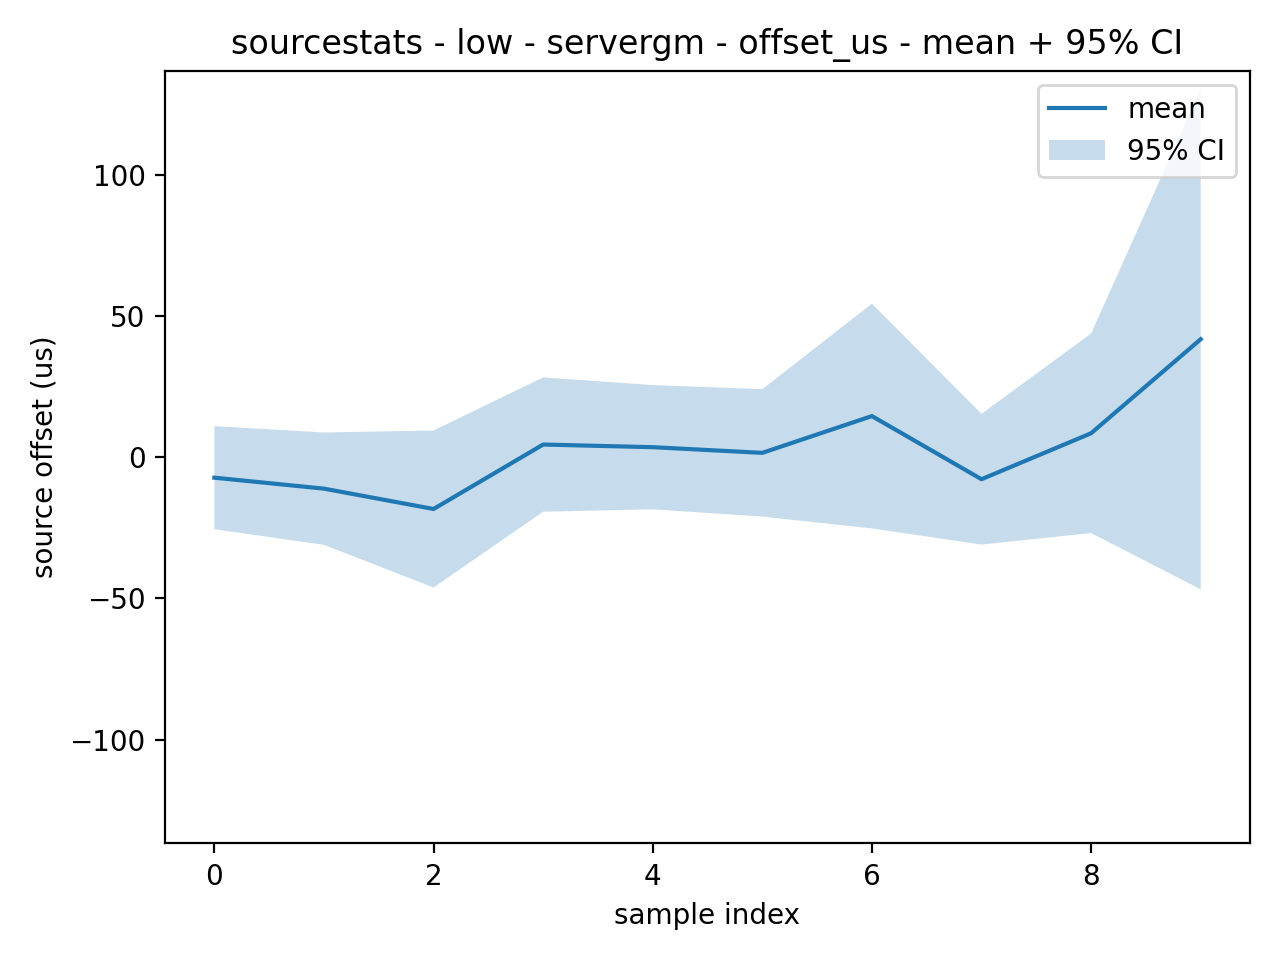
\includegraphics[width=\linewidth]{
      pars_plots/chrony_servergm/_aggregated/sourcestats/low/servergm/offset_us_mean_ci95.png
    }
    \caption{Scenario LOW}
  \end{subfigure}
  \hfill
  \begin{subfigure}
    {0.32\textwidth}
    \centering
    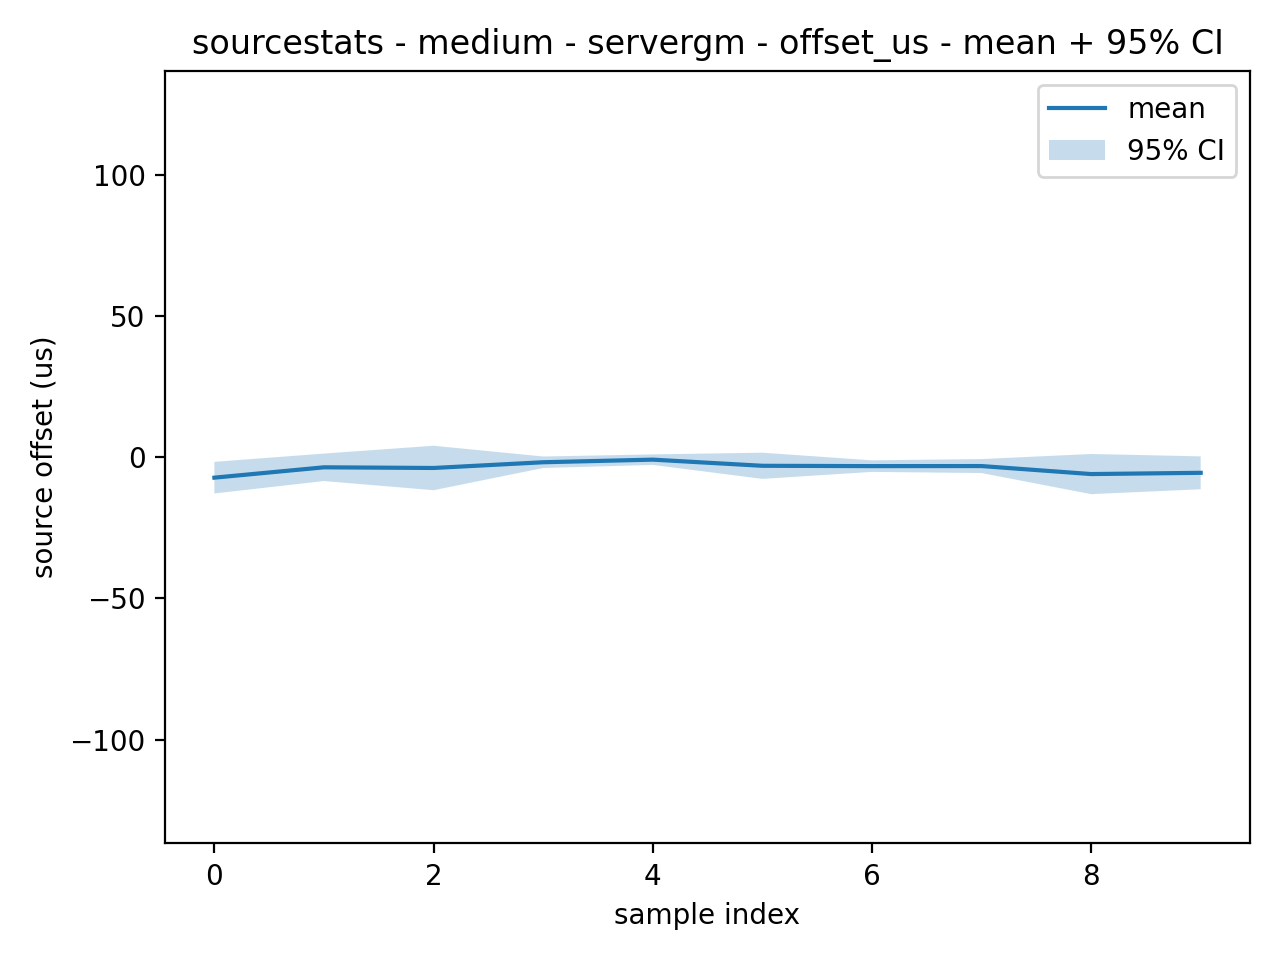
\includegraphics[width=\linewidth]{
      pars_plots/chrony_servergm/_aggregated/sourcestats/medium/servergm/offset_us_mean_ci95.png
    }
    \caption{Scenario MEDIUM}
  \end{subfigure}
  \begin{subfigure}
    {0.32\textwidth}
    \centering
    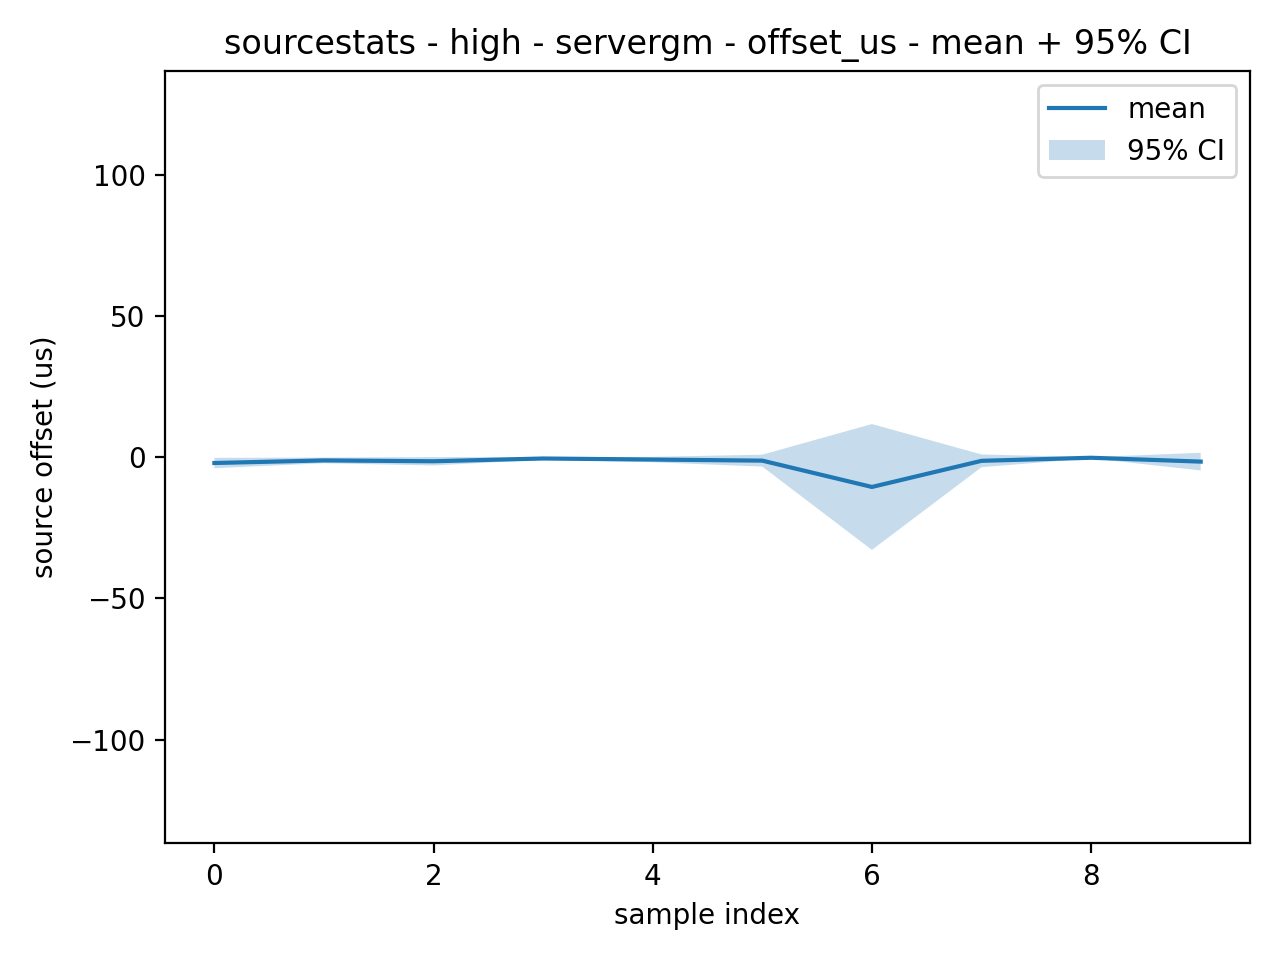
\includegraphics[width=\linewidth]{
      pars_plots/chrony_servergm/_aggregated/sourcestats/high/servergm/offset_us_mean_ci95.png
    }
    \caption{Scenario HIGH}
  \end{subfigure}
  \caption{Media con intervallo di confidenza al 95\% - nodo: \texttt{clientchrony}
  - netem/tc: \texttt{servergm}}
  \label{fig:scenario_comparison}
\end{figure}
\begin{figure}[H]
  \centering

  \begin{subfigure}
    {0.32\textwidth}
    \centering
    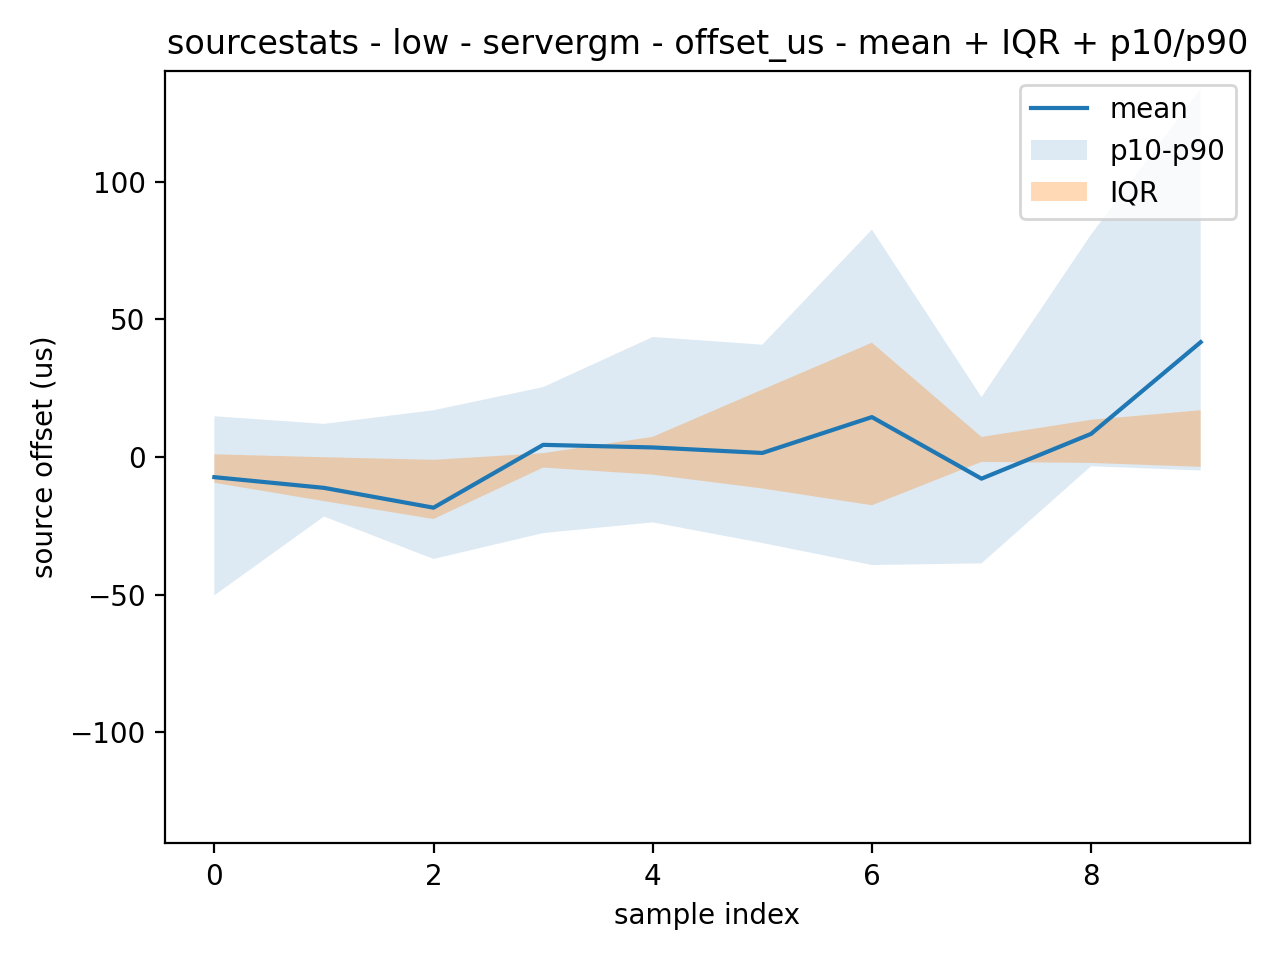
\includegraphics[width=\linewidth]{
      pars_plots/chrony_servergm/_aggregated/sourcestats/low/servergm/offset_us_mean_iqr_p10_p90.png
    }
    \caption{Scenario LOW}
  \end{subfigure}
  \hfill
  \begin{subfigure}
    {0.32\textwidth}
    \centering
    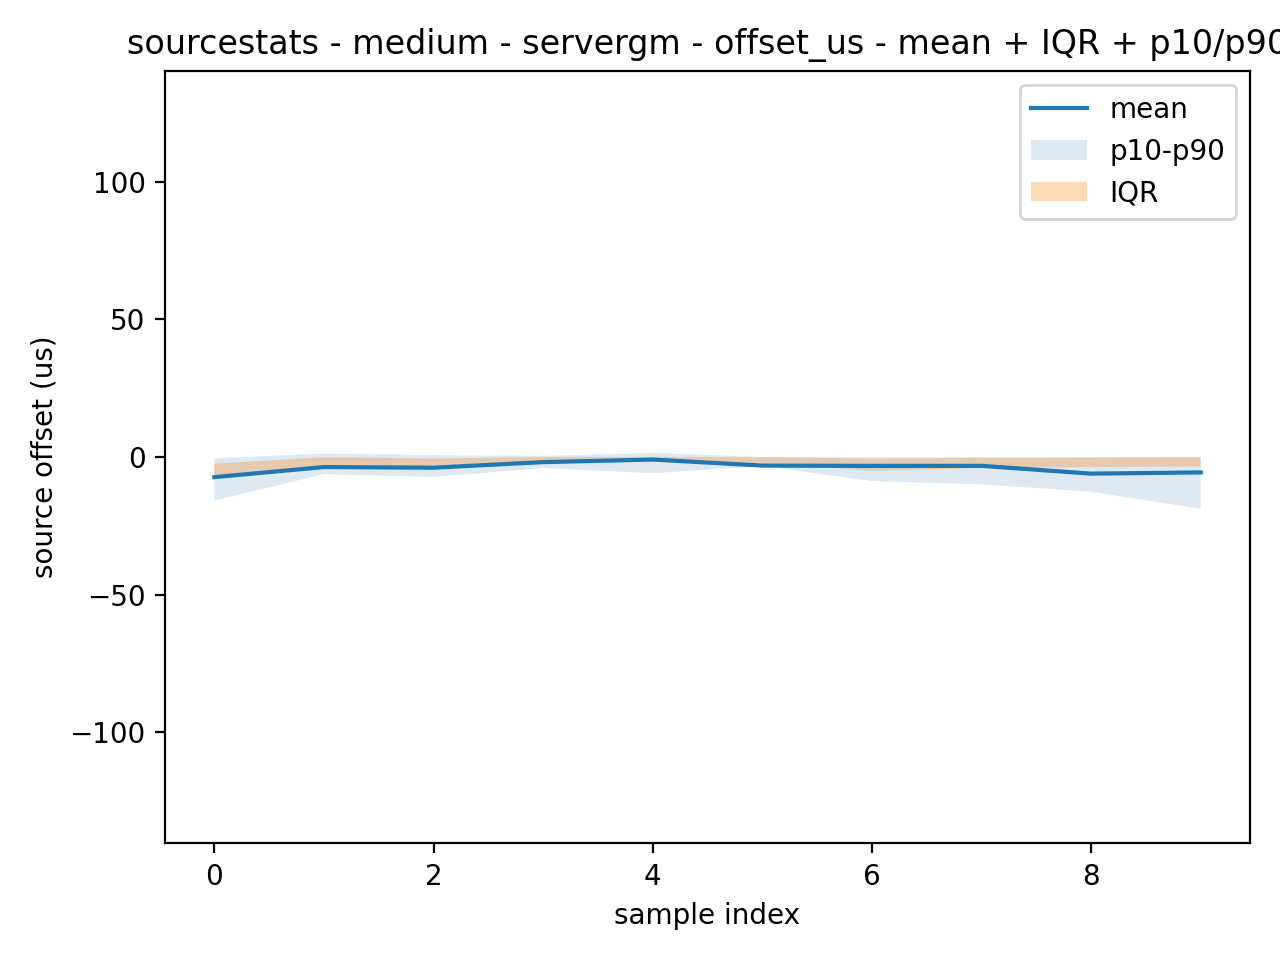
\includegraphics[width=\linewidth]{
      pars_plots/chrony_servergm/_aggregated/sourcestats/medium/servergm/offset_us_mean_iqr_p10_p90.png
    }
    \caption{Scenario MEDIUM}
  \end{subfigure}
  \begin{subfigure}
    {0.32\textwidth}
    \centering
    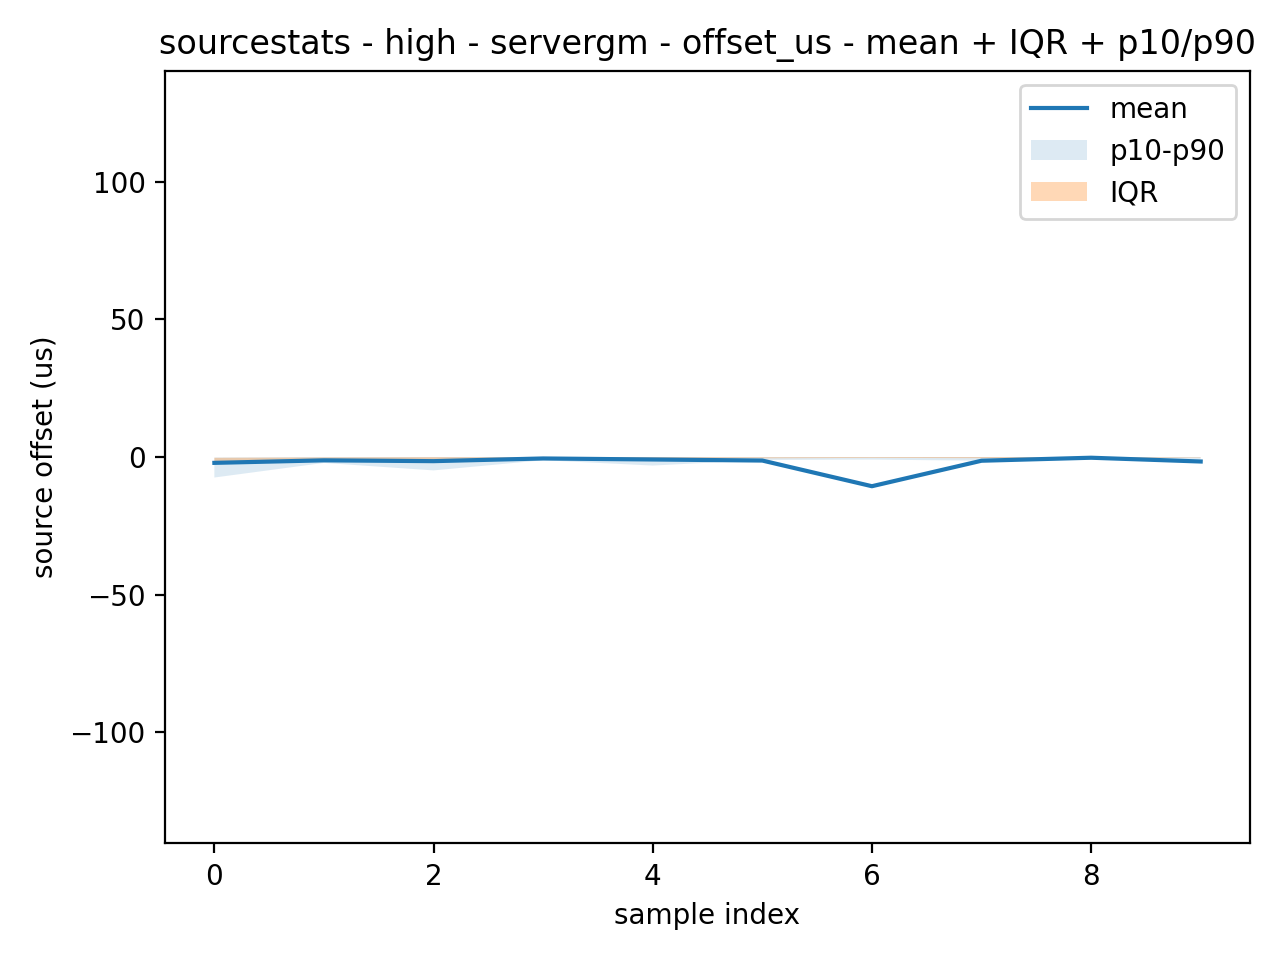
\includegraphics[width=\linewidth]{
      pars_plots/chrony_servergm/_aggregated/sourcestats/high/servergm/offset_us_mean_iqr_p10_p90.png
    }
    \caption{Scenario HIGH}
  \end{subfigure}
  \caption{Media con banda inter-quartile e banda p10-p90 - nodo: \texttt{clientchrony}
  - netem/tc: \texttt{servergm}}
  \label{fig:scenario_comparison}
\end{figure}
\paragraph*{servergm - netem/tc:}
La \texttt{offset\_us} riferita alla sezione \texttt{sourcestats}, l'evidenzia
un comportamento non monotono al variare dello scenario, ma nel complesso compatibile
con una sincronizzazione che resta attiva e generalmente prossima alla sorgente di
riferimento.

Nello scenario \texttt{low}. Il valor medio è di ~\texttt{2.935 \,$\mu$s},
prossimo allo zero, La deviazione standard delle medie è \texttt{16.824 \,$\mu$s},
con valori in un intervallo di \texttt{-18.383 \,$\mu$s} e \texttt{41.717 \,$\mu$s}.
Le bande di variabilità sono ampie, con una larghezza media dell'intervallo \texttt{p10-p90}
pari a \texttt{74.976 \,$\mu$s} con presenza di picchi fino a \texttt{138.489 \,$\mu$s}.
Il comportamento nello scenario \texttt{low} è caratterizzato da variabilità
inter-run e da outlier positivi che ampliano sensibilmente la dispersione
osservata.

Nel caso \texttt{medium}, c'è un comportamento più regolare. Si ha una media aggregata
di ~\texttt{-3.863 \,$\mu$s}. La dispersione è ridotta notevolmente la deviazione
standard delle medie scende a \texttt{1.935 \,$\mu$s}, mentre l'intervallo medio
\texttt{p10-p90} è di ~\texttt{9.546 \,$\mu$s}.In questo caso l'offset contenuto vicino
allo zero e mostra una variabilità minore rispetto al caso precedente.

Nello scenario \texttt{high} si ha un comportamento stabile. La media aggregata della
curva è pari a \texttt{-2.122 \,$\mu$s}. La deviazione standard delle medie è \texttt{3.022
\,$\mu$s}. L'ampiezza media dell'IQR è di ~\texttt{0.709 \,$\mu$s}, mentre l'intervallo
medio \texttt{p10-p90} è pari a \texttt{2.355 \,$\mu$s}, valori che descrivono una
forte concentrazione della parte centrale della distribuzione. Nel grafico è
visibile una singola flessione più marcata, coerente con il minimo della curva pari
a \texttt{-10.588 \,$\mu$s}.

Nel confronto complessivo non c'è un risultato lineare. Il caso \texttt{low}
mostra maggiore dispersione con valori anomali, mantenendo comunque valori prossimi
allo zero. I casi \texttt{medium} e \texttt{high} appaiono invece più regolari. Tale
metrica non produce una deriva sistematica progressivamente crescente al variare dello
scenario.

\paragraph*{Confronto:}
L'impairment introdotto su \texttt{clientchrony} si hanno valori sulla metrica più
coerenti: al crescere dello scenario si osserva un progressivo peggioramento, con
medie che si spostano verso valori più negativi e con un aumento della dispersione. Nel
caso invece di \texttt{servergm}, il comportamento appare meno regolare e non monotono.
In sintesi, applicando il degrado sul lato client si manifestano dati più coerenti
con le aspettative.

\subsection{Analisi metrica: \texttt{stddev}}
\begin{figure}[H]
  \centering

  \begin{subfigure}
    {0.32\textwidth}
    \centering
    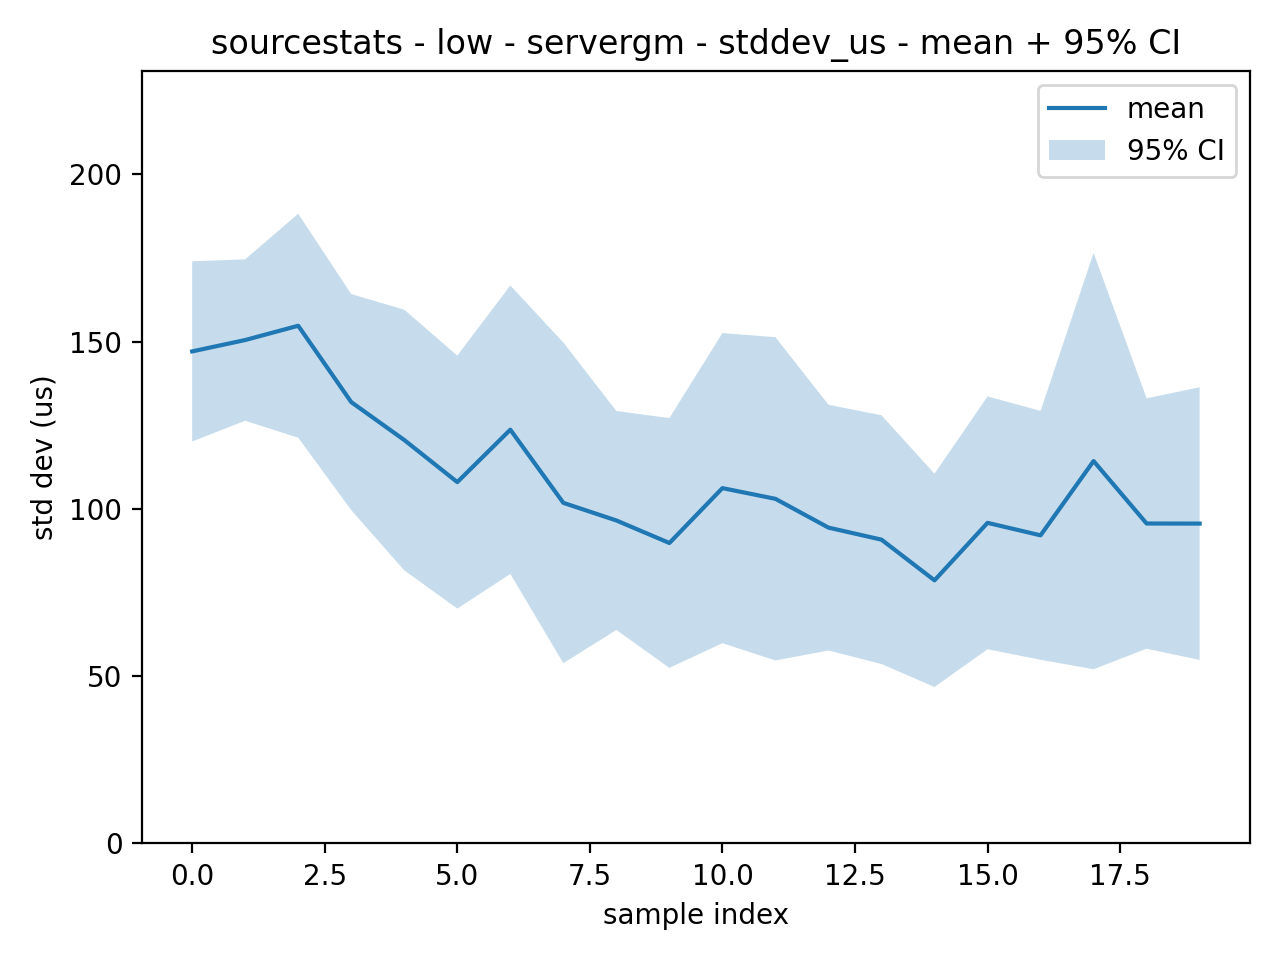
\includegraphics[width=\linewidth]{
      pars_plots/chrony_clientchrony/_aggregated/sourcestats/low/servergm/stddev_us_mean_ci95.png
    }
    \caption{Scenario LOW}
  \end{subfigure}
  \hfill
  \begin{subfigure}
    {0.32\textwidth}
    \centering
    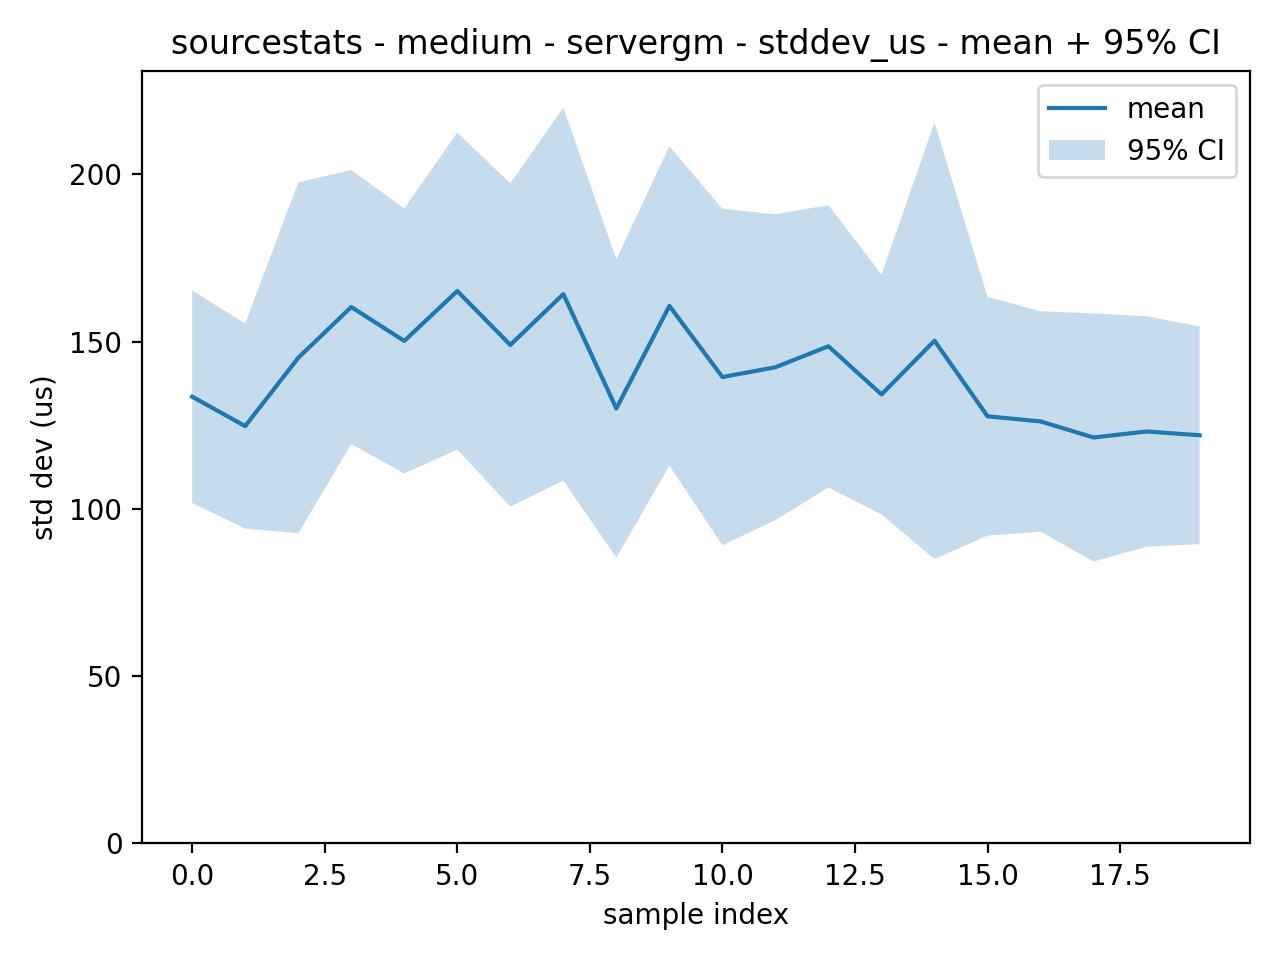
\includegraphics[width=\linewidth]{
      pars_plots/chrony_clientchrony/_aggregated/sourcestats/medium/servergm/stddev_us_mean_ci95.png
    }
    \caption{Scenario MEDIUM}
  \end{subfigure}
  \begin{subfigure}
    {0.32\textwidth}
    \centering
    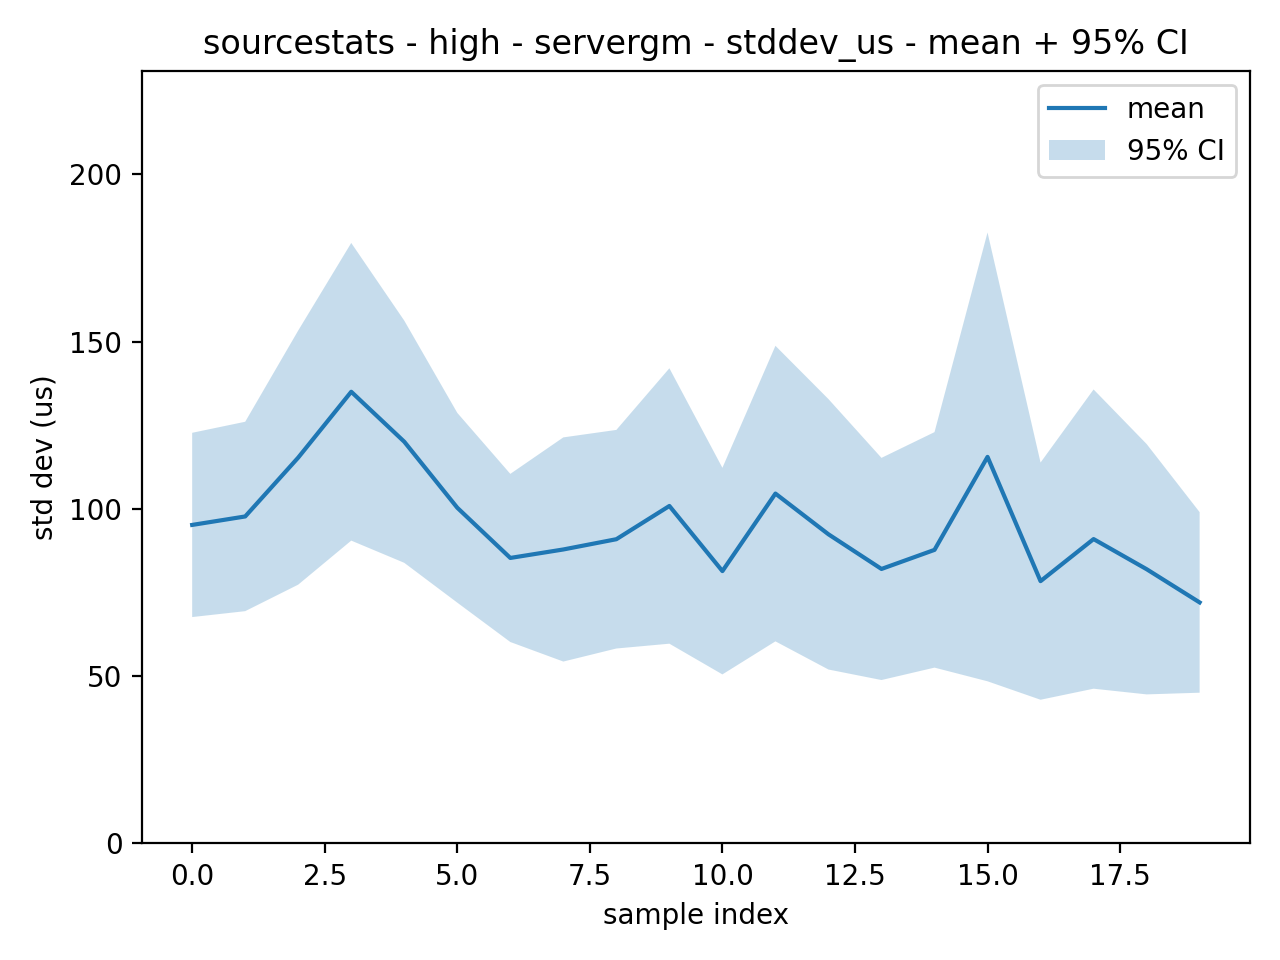
\includegraphics[width=\linewidth]{
      pars_plots/chrony_clientchrony/_aggregated/sourcestats/high/servergm/stddev_us_mean_ci95.png
    }
    \caption{Scenario HIGH}
  \end{subfigure}
  \caption{Media con intervallo di confidenza al 95\% - nodo: \texttt{clientchrony}
  - netem/tc: \texttt{clientchrony}}
  \label{fig:scenario_comparison}
\end{figure}
\begin{figure}[H]
  \centering

  \begin{subfigure}
    {0.32\textwidth}
    \centering
    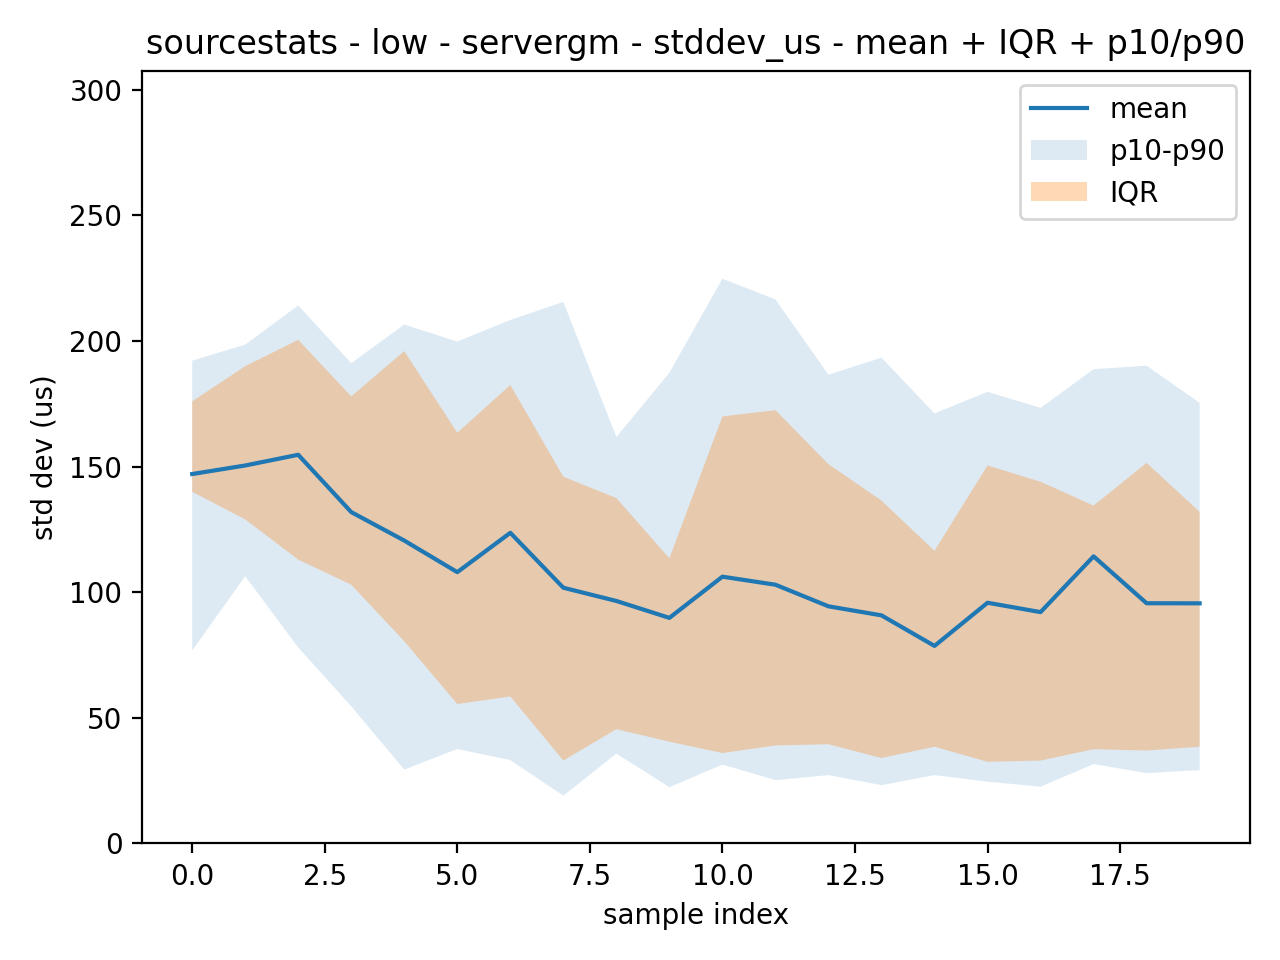
\includegraphics[width=\linewidth]{
      pars_plots/chrony_clientchrony/_aggregated/sourcestats/low/servergm/stddev_us_mean_iqr_p10_p90.png
    }
    \caption{Scenario LOW}
  \end{subfigure}
  \hfill
  \begin{subfigure}
    {0.32\textwidth}
    \centering
    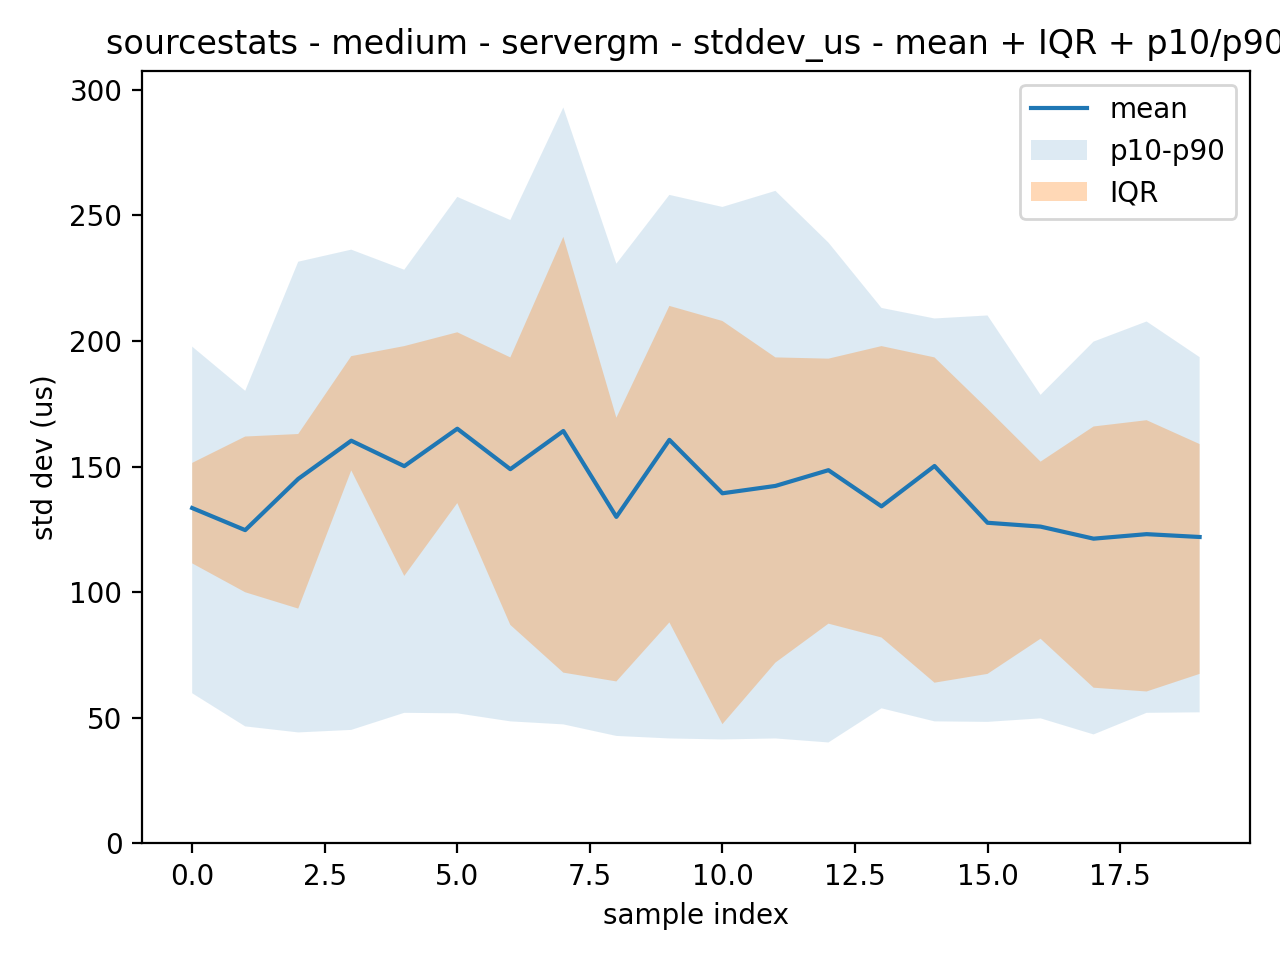
\includegraphics[width=\linewidth]{
      pars_plots/chrony_clientchrony/_aggregated/sourcestats/medium/servergm/stddev_us_mean_iqr_p10_p90.png
    }
    \caption{Scenario MEDIUM}
  \end{subfigure}
  \begin{subfigure}
    {0.32\textwidth}
    \centering
    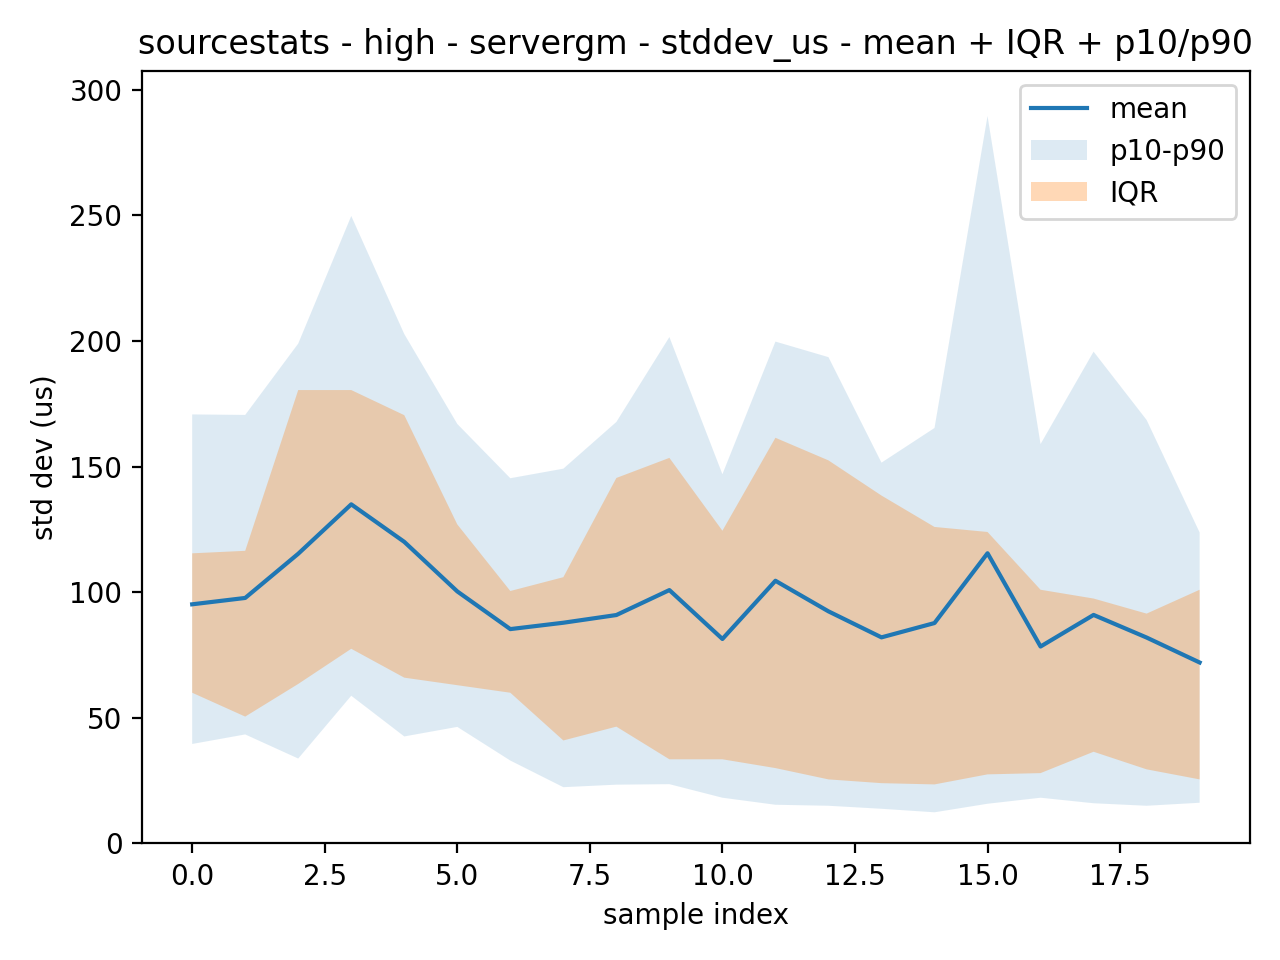
\includegraphics[width=\linewidth]{
      pars_plots/chrony_clientchrony/_aggregated/sourcestats/high/servergm/stddev_us_mean_iqr_p10_p90.png
    }
    \caption{Scenario HIGH}
  \end{subfigure}
  \caption{Media con banda inter-quartile e banda p10-p90 - nodo: \texttt{clientchrony}
  - netem/tc: \texttt{clientchrony}}
  \label{fig:scenario_comparison}
\end{figure}
\paragraph*{clientchrony - netem/tc:}
Per la metrica \texttt{stddev\_us}, il caso \texttt{clientchrony} non è presente una variazione
monotona crescente, ma piuttosto una risposta non lineare della variabilità
stimata rispetto alla sorgente. In tutti i casi i valori restano dell'ordine delle
centinaia di microsecondi.

Nello scenario \texttt{low} si ha una media aggregata di ~\texttt{109.552 \,$\mu$s}.
La dispersione non è trascurabile. La deviazione standard delle medie è di ~\texttt{21.838
\,$\mu$s}, in un intervallo d \texttt{78.637 \,$\mu$s} e \texttt{154.733 \,$\mu$s}.
Ci sono bande relativamente ampie, con IQR medio di ~\texttt{98.925 \,$\mu$s} e
ampiezza media \texttt{p10-p90} pari a \texttt{155.630 \,$\mu$s}. La mediana è ~\texttt{103
\,$\mu$s}, il terzo quartile \texttt{167 \,$\mu$s} e il massimo \texttt{464 \,$\mu$s}.

Nel caso \texttt{medium} si ha una crescita dei valori. La media aggregata è di
~\texttt{140.899 \,$\mu$s}. La mediana della curva è di ~\texttt{140.867 \,$\mu$s}
con valori che oscillano nell'intervallo \texttt{121.333 \,$\mu$s} e \texttt{165.109
\,$\mu$s}. La deviazione standard delle medie è \texttt{14.774 \,$\mu$s}. Le
bande di variabilità risultano tuttavia più larghe del caso \texttt{low}: l'IQR
medio sale a \texttt{100.000 \,$\mu$s} e l'ampiezza media \texttt{p10-p90}
raggiunge \texttt{178.740 \,$\mu$s}. Si ha un terzo quartile di\texttt{191.250
\,$\mu$s} e un massimo di \texttt{510 \,$\mu$s}.

Nello scenario \texttt{high} la media aggregata della curva è di ~\texttt{95.787
\,$\mu$s}, con mediana \texttt{91.687 \,$\mu$s}. L'IQR medio vale \texttt{88.450
\,$\mu$s}, mentre l'ampiezza media \texttt{p10-p90} è pari a \texttt{154.760 \,$\mu$s},
dunque molto vicina al caso \texttt{low} ma inferiore al caso \texttt{medium}. I dati
mostrano una riduzione del livello medio, con media complessiva \texttt{95.787
\,$\mu$s}, mediana \texttt{88 \,$\mu$s} e massimo \texttt{410 \,$\mu$s}.

Lo scenario \texttt{medium} è quello che presenta il livello medio più elevato,
\texttt{low} occupa una posizione intermedia e \texttt{high} mostra invece valori
medi più contenuti. Anche sul piano della dispersione intra-curva e inter-run non
si osserva una crescita progressiva con l'intensità del degrado. Pertanto, per questa
metrica, il degrado applicato su \texttt{clientchrony} non produce una risposta semplicemente
crescente, ma modifica la stima della deviazione standard in modo più articolato,
con un massimo nel caso \texttt{medium} e un successivo ridimensionamento nel
caso \texttt{high}.

\begin{figure}[H]
  \centering

  \begin{subfigure}
    {0.32\textwidth}
    \centering
    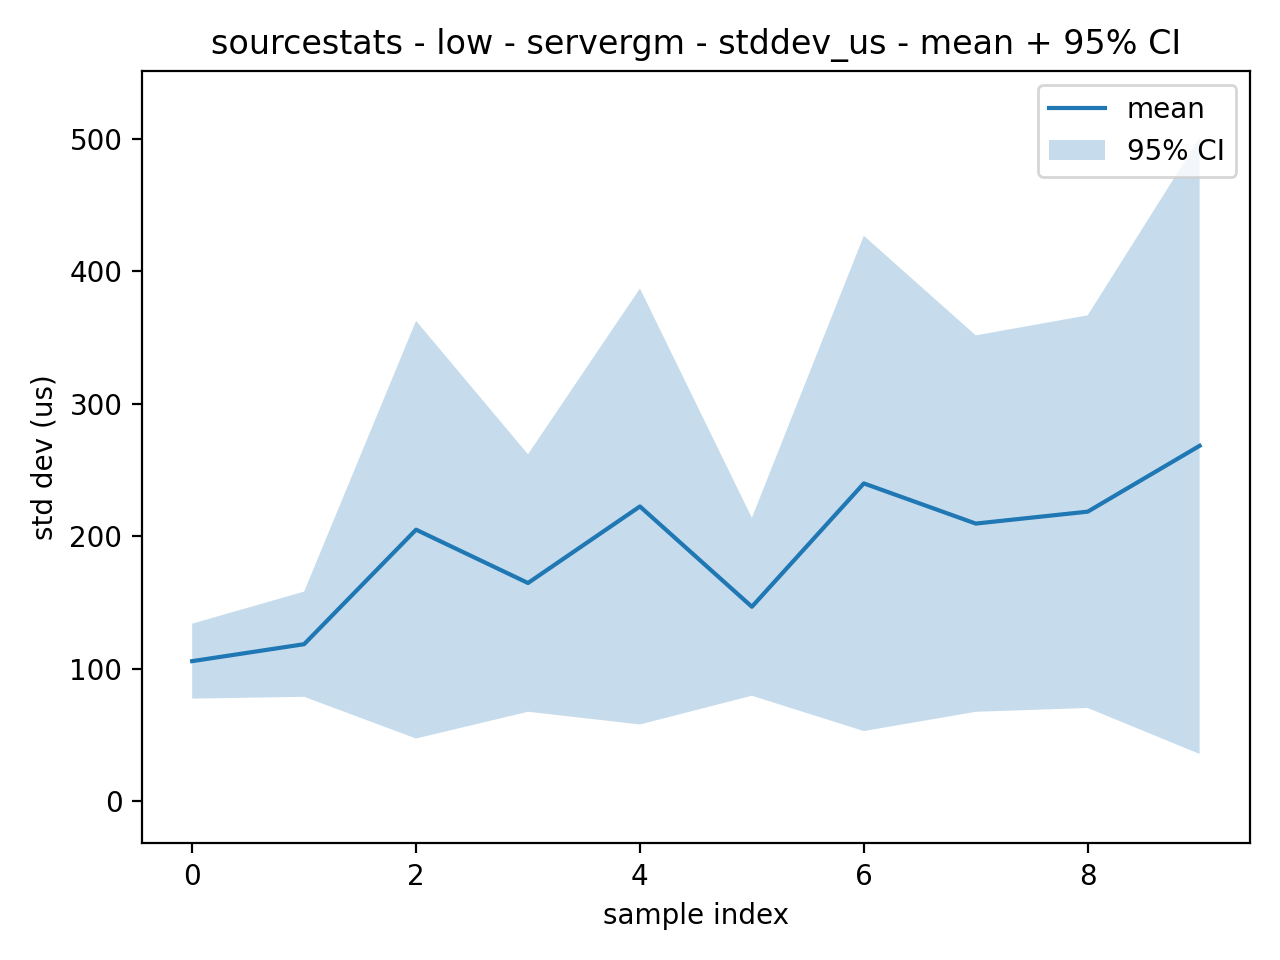
\includegraphics[width=\linewidth]{
      pars_plots/chrony_servergm/_aggregated/sourcestats/low/servergm/stddev_us_mean_ci95.png
    }
    \caption{Scenario LOW}
  \end{subfigure}
  \hfill
  \begin{subfigure}
    {0.32\textwidth}
    \centering
    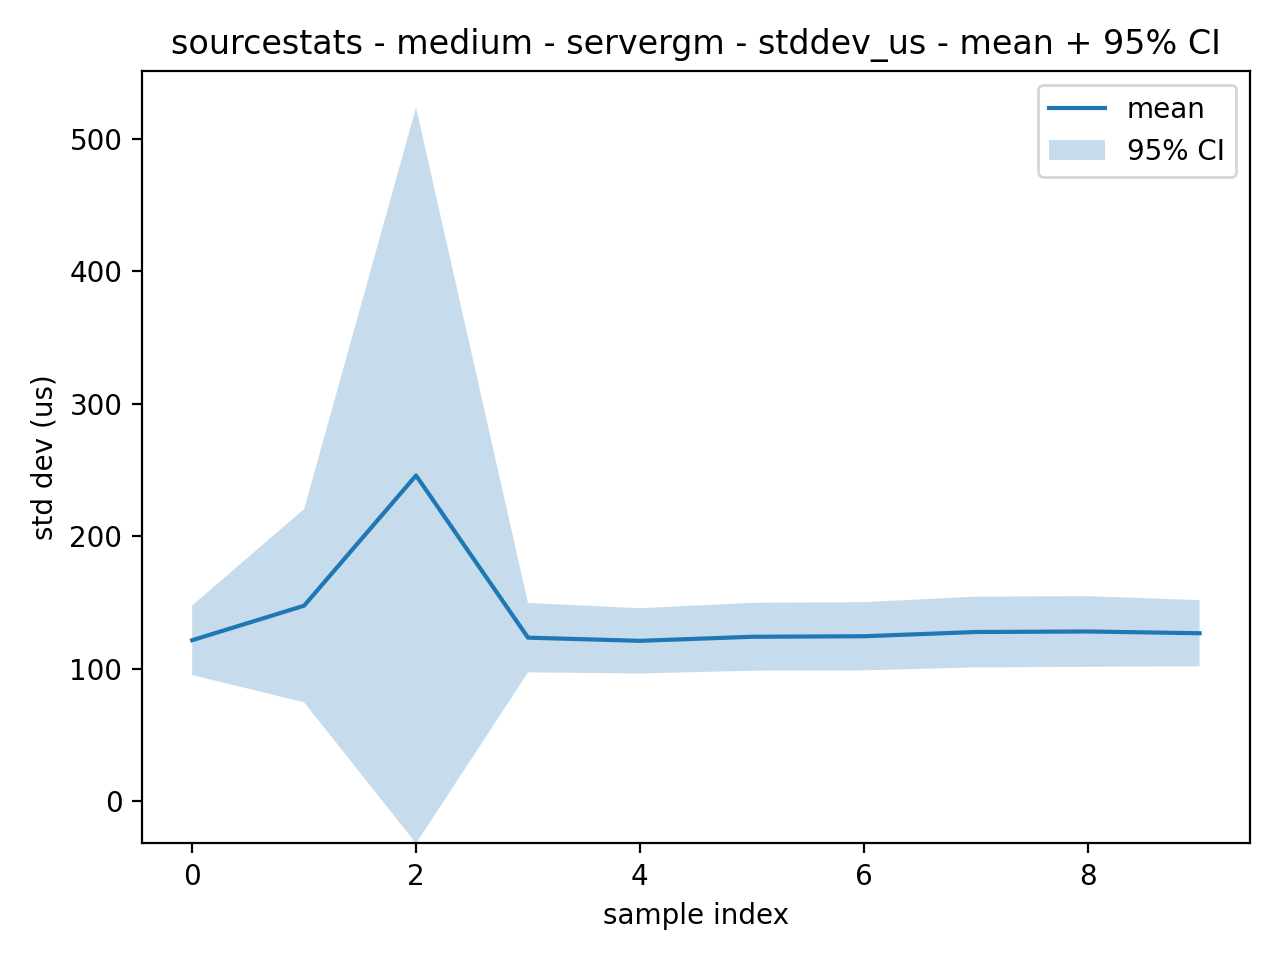
\includegraphics[width=\linewidth]{
      pars_plots/chrony_servergm/_aggregated/sourcestats/medium/servergm/stddev_us_mean_ci95.png
    }
    \caption{Scenario MEDIUM}
  \end{subfigure}
  \begin{subfigure}
    {0.32\textwidth}
    \centering
    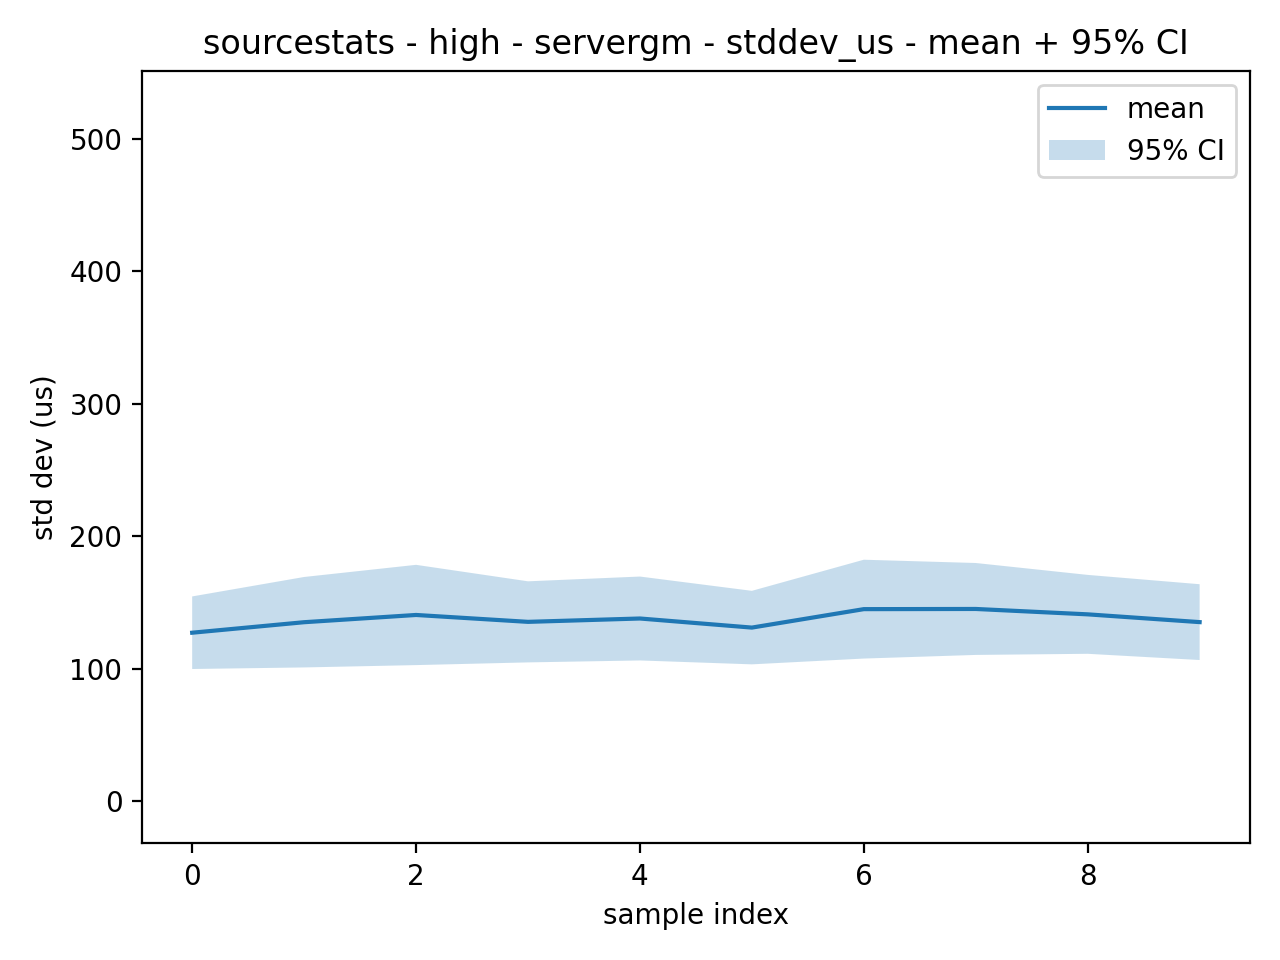
\includegraphics[width=\linewidth]{
      pars_plots/chrony_servergm/_aggregated/sourcestats/high/servergm/stddev_us_mean_ci95.png
    }
    \caption{Scenario HIGH}
  \end{subfigure}
  \caption{Media con intervallo di confidenza al 95\% - nodo: \texttt{clientchrony}
  - netem/tc: \texttt{servergm}}
  \label{fig:scenario_comparison}
\end{figure}
\begin{figure}[H]
  \centering

  \begin{subfigure}
    {0.32\textwidth}
    \centering
    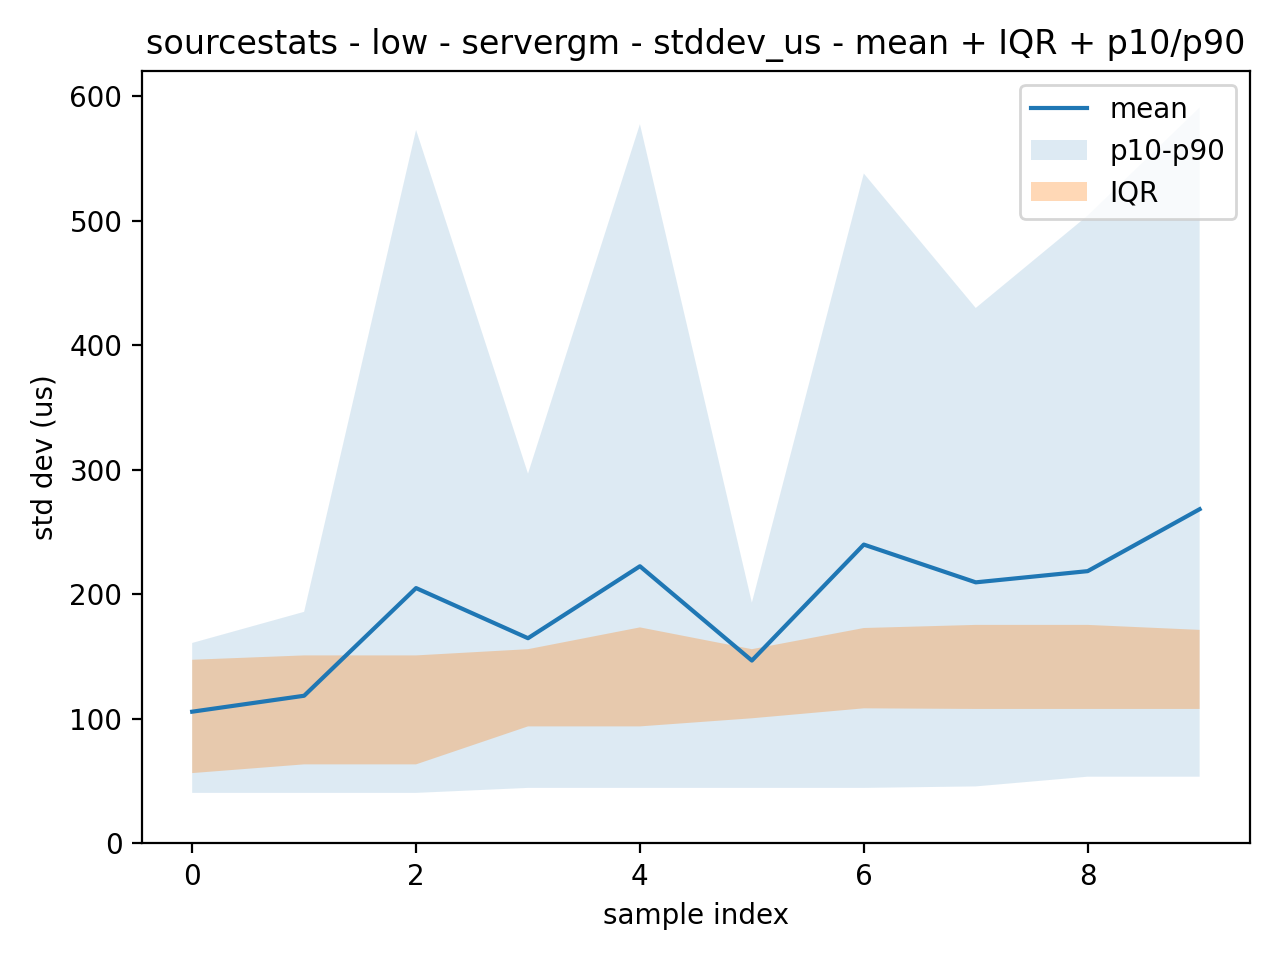
\includegraphics[width=\linewidth]{
      pars_plots/chrony_servergm/_aggregated/sourcestats/low/servergm/stddev_us_mean_iqr_p10_p90.png
    }
    \caption{Scenario LOW}
  \end{subfigure}
  \hfill
  \begin{subfigure}
    {0.32\textwidth}
    \centering
    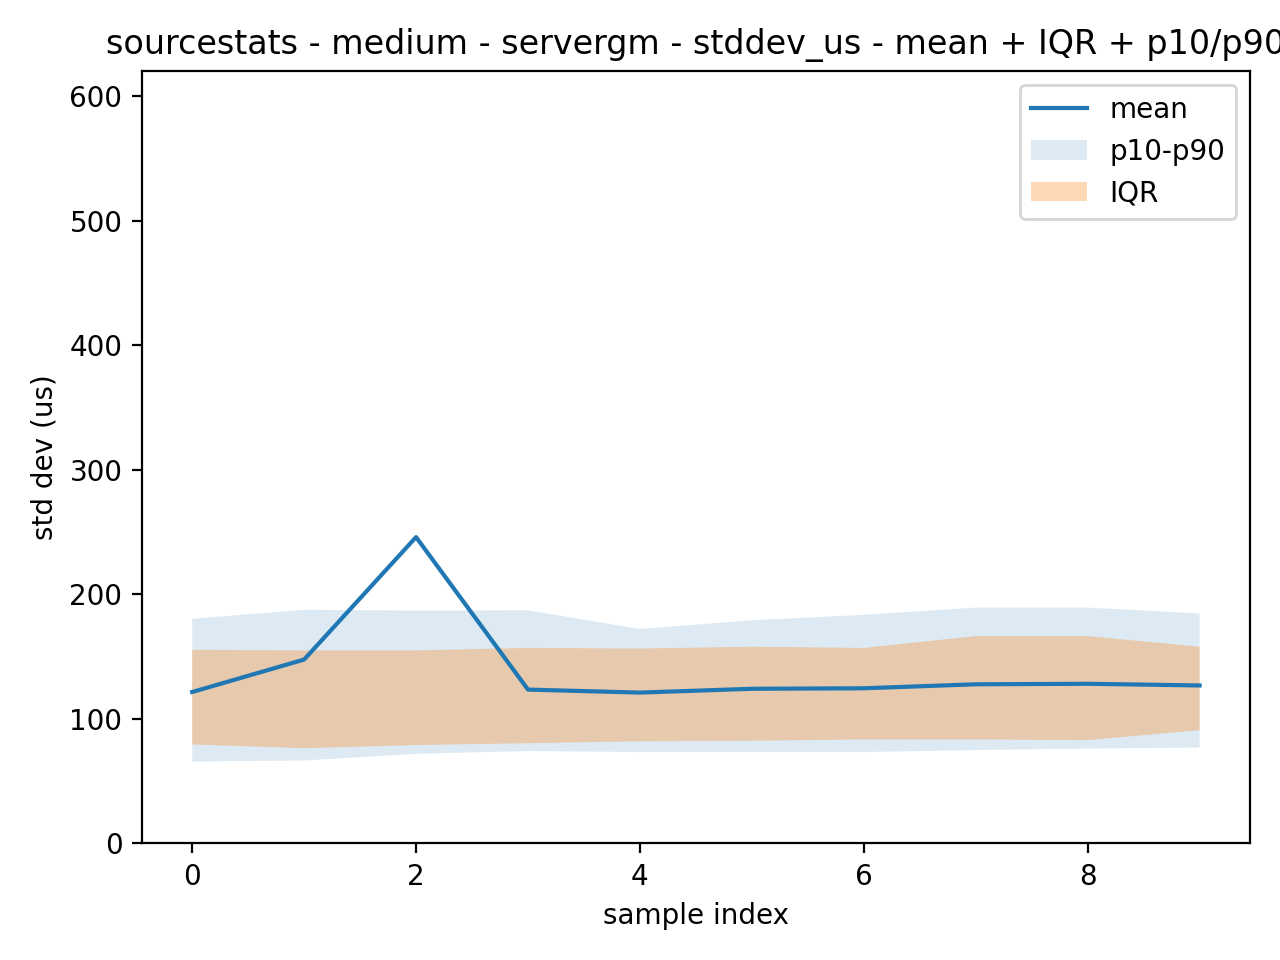
\includegraphics[width=\linewidth]{
      pars_plots/chrony_servergm/_aggregated/sourcestats/medium/servergm/stddev_us_mean_iqr_p10_p90.png
    }
    \caption{Scenario MEDIUM}
  \end{subfigure}
  \begin{subfigure}
    {0.32\textwidth}
    \centering
    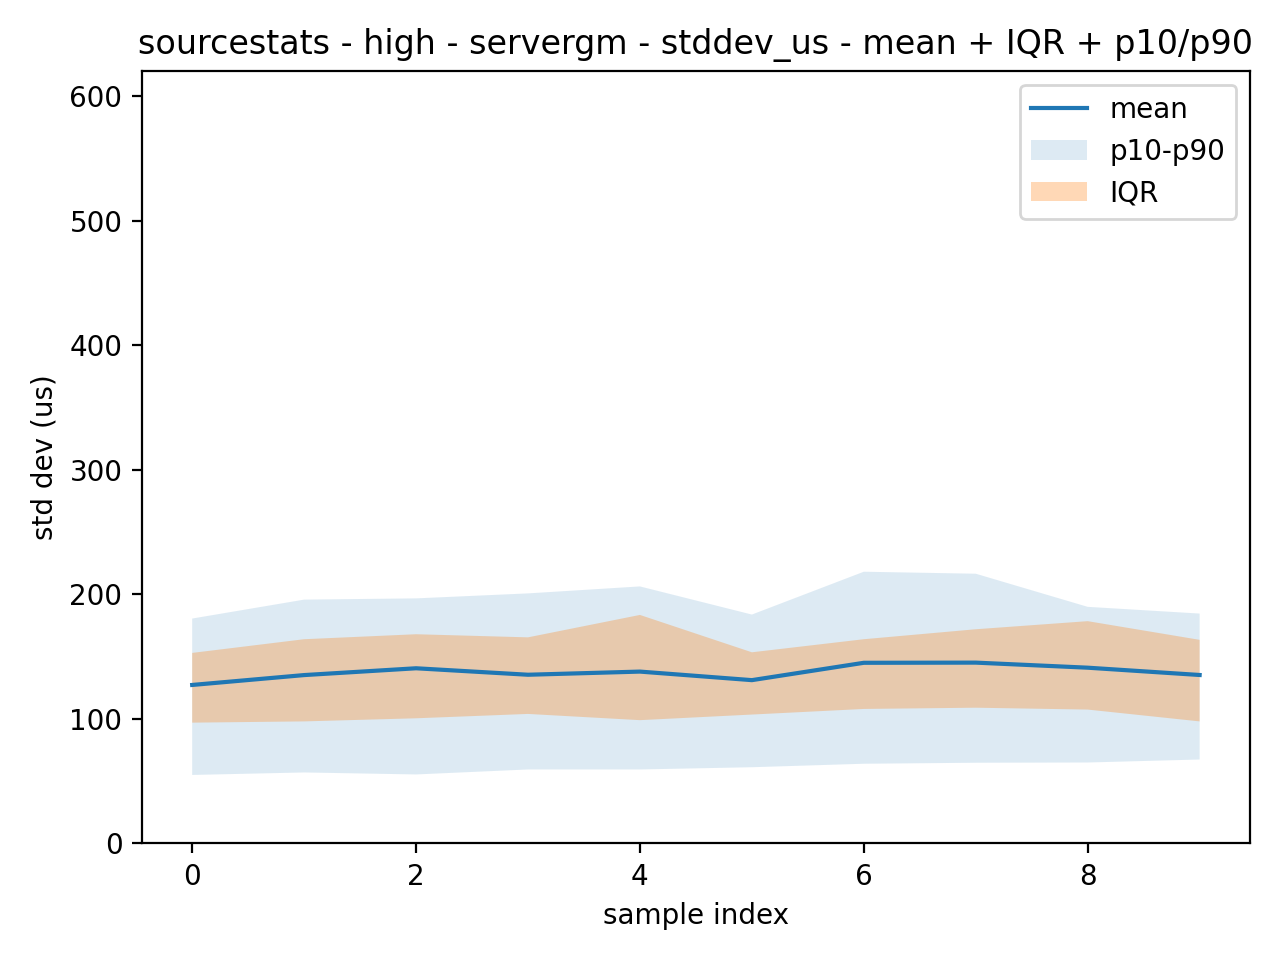
\includegraphics[width=\linewidth]{
      pars_plots/chrony_servergm/_aggregated/sourcestats/high/servergm/stddev_us_mean_iqr_p10_p90.png
    }
    \caption{Scenario HIGH}
  \end{subfigure}
  \caption{Media con banda inter-quartile e banda p10-p90 - nodo: \texttt{clientchrony}
  - netem/tc: \texttt{servergm}}
  \label{fig:scenario_comparison}
\end{figure}

\paragraph*{servergm - netem/tc:}
Nello scenario \texttt{low} la media aggregata è \texttt{190.047 \,$\mu$s} e la deviazione
standard delle medie è di \texttt{53.570 \,$\mu$s}. L'IQR medio è di \texttt{72.600
\,$\mu$s}, e l'ampiezza media dell'intervallo \texttt{p10-p90} raggiunge \texttt{359.800
\,$\mu$s}, con picchi fino a \texttt{537.400 \,$\mu$s}. Si ha un massimo di
\texttt{1622 \,$\mu$s}. Nel complesso, quindi, lo scenario \texttt{low} descrive una
stima della deviazione standard elevata e accompagnata da una variabilità molto marcata
tra le run. In tale scenario, la media è più affetta dagli outlier che dai valori tipici, 
si nota dalla presenza di un valore medio che si discosta dalla banda inter-quartile.

Nel caso \texttt{medium} la media aggregata della curva è di \texttt{139.160 \,$\mu$s}.
La deviazione standard delle medie è di \texttt{38.298 \,$\mu$s}. I valori medi
risultano compresi tra \texttt{121.133 \,$\mu$s} e \texttt{246.000 \,$\mu$s}. L'IQR
medio vale \texttt{76.400 \,$\mu$s}, mentre l'intervallo medio \texttt{p10-p90}
è pari a \texttt{111.360 \,$\mu$s}. Si ha una mediana di \texttt{130 \,$\mu$s}.
Il massimo pari a \texttt{2053 \,$\mu$s}

Nello scenario \texttt{high} la media aggregata è pari a \texttt{137.440 \,$\mu$s}.
La deviazione standard delle medie scende drasticamente a \texttt{5.770 \,$\mu$s}.
Anche l'intervallo dei valori medi lungo la curva risulta molto ristretto,
compreso tra \texttt{127.267 \,$\mu$s} e \texttt{145.200 \,$\mu$s}. Le bande di dispersione
si contraggono: l'IQR medio è pari a \texttt{64.100 \,$\mu$s} e l'ampiezza media \texttt{p10-p90}
è \texttt{136.500 \,$\mu$s}.

Non è presente una dinamica lineare nel confronto. Il caso \texttt{low} la maggiore
dispersione. I casi \texttt{medium} e \texttt{high} mostrano invece medie
inferiori e molto simili tra loro, ma differiscono sul piano della stabilità.

\paragraph*{Confronto:}
L'impairment sul server tende a produrre un effetto più severo soprattutto nel
caso \texttt{low}, accompagnato da una dispersione molto marcata e da outlier
più pronunciati. L'impairment sul client mostra invece un comportamento più regolare,
con variazioni meno estreme e una risposta non monotona centrata sul caso
\texttt{medium}.

\subsection{Analisi metrica: \texttt{system time offset}}
\begin{figure}[H]
  \centering

  \begin{subfigure}
    {0.32\textwidth}
    \centering
    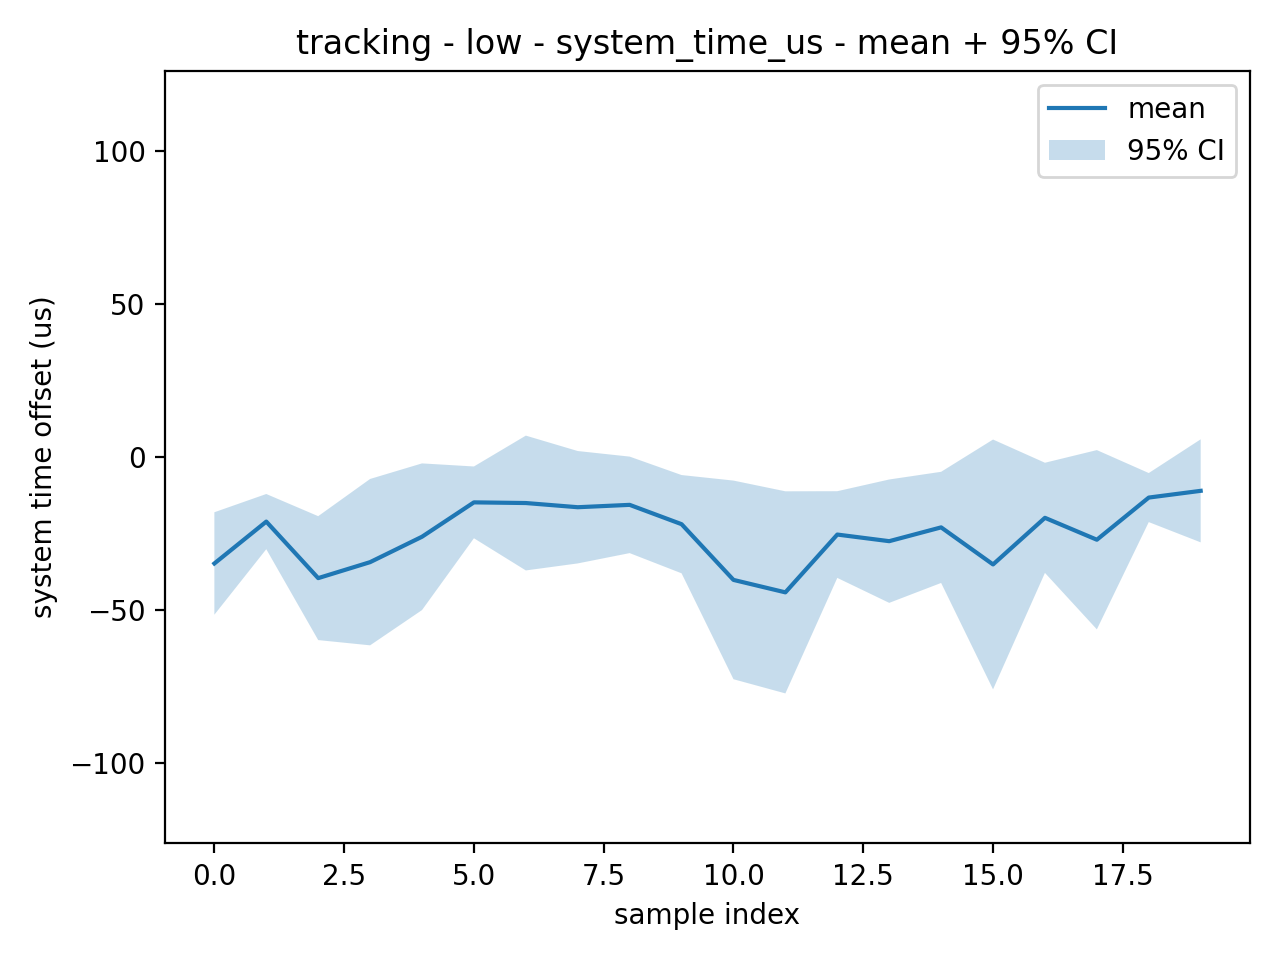
\includegraphics[width=\linewidth]{
      pars_plots/chrony_clientchrony/_aggregated/tracking/low/system_time_us_mean_ci95.png
    }
    \caption{Scenario LOW}
  \end{subfigure}
  \hfill
  \begin{subfigure}
    {0.32\textwidth}
    \centering
    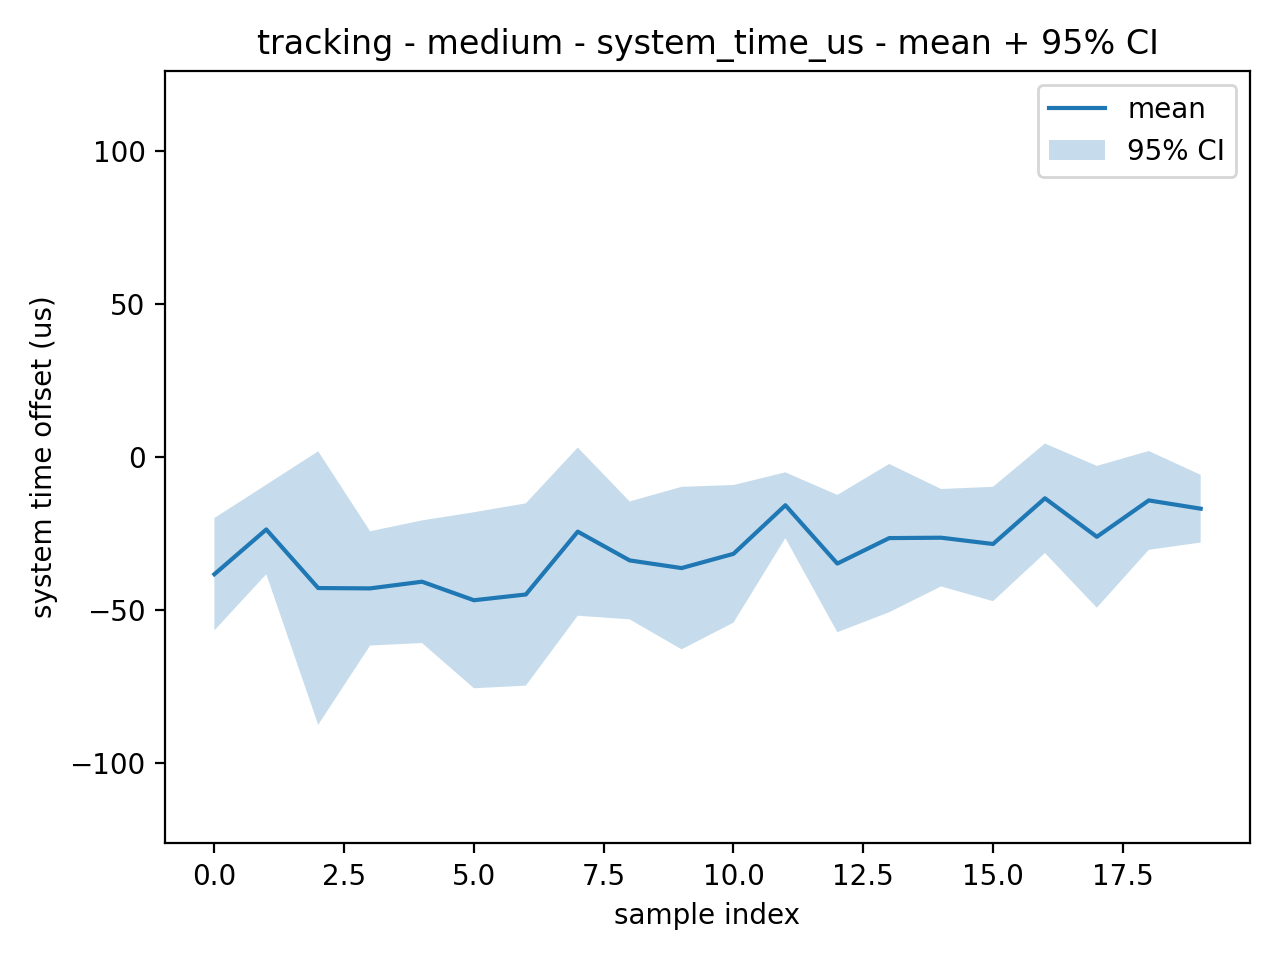
\includegraphics[width=\linewidth]{
      pars_plots/chrony_clientchrony/_aggregated/tracking/medium/system_time_us_mean_ci95.png
    }
    \caption{Scenario MEDIUM}
  \end{subfigure}
  \begin{subfigure}
    {0.32\textwidth}
    \centering
    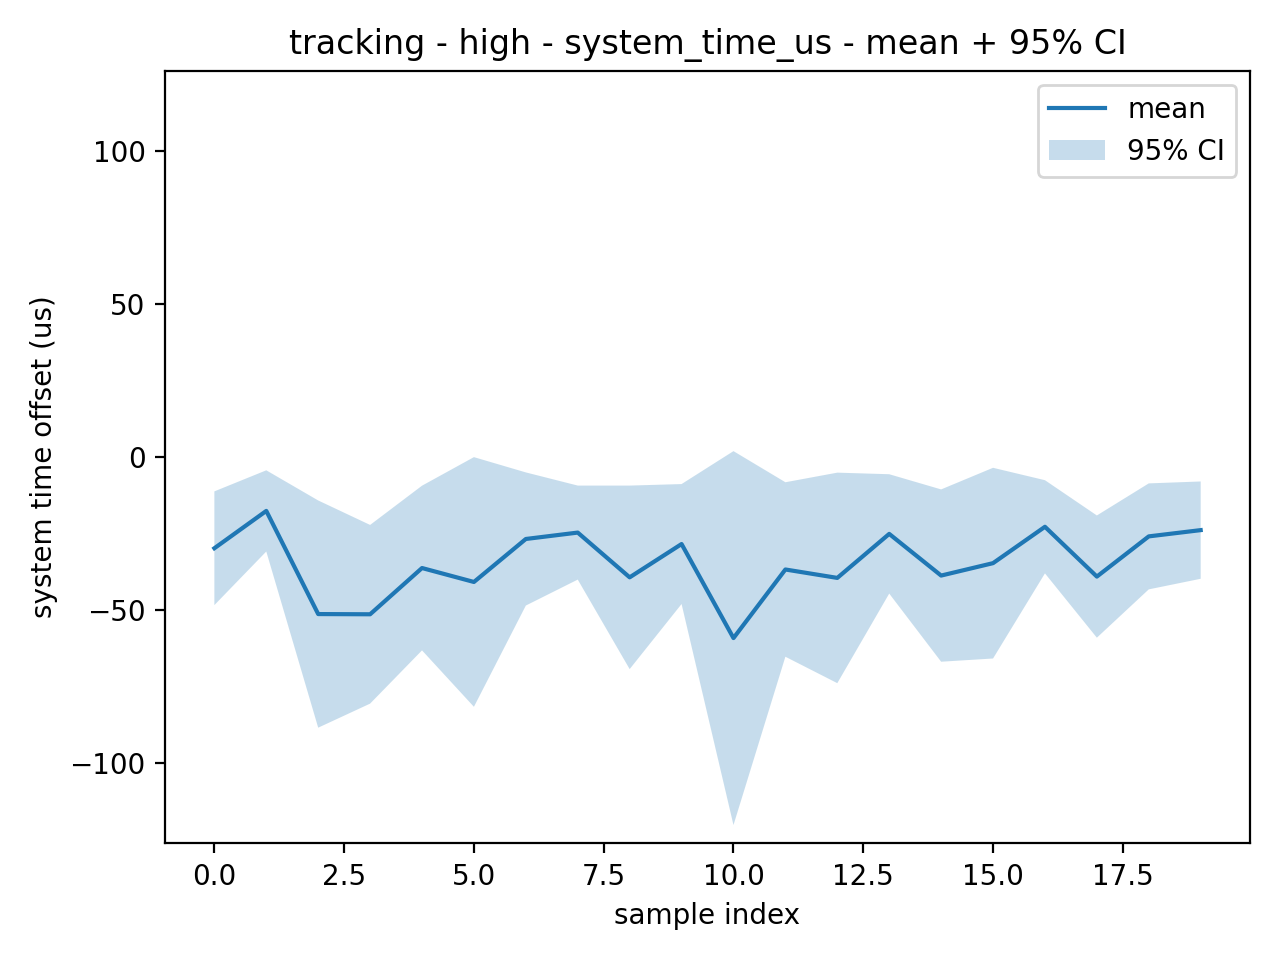
\includegraphics[width=\linewidth]{
      pars_plots/chrony_clientchrony/_aggregated/tracking/high/system_time_us_mean_ci95.png
    }
    \caption{Scenario HIGH}
  \end{subfigure}
  \caption{Media con intervallo di confidenza al 95\% - nodo: \texttt{clientchrony}
  - netem/tc: \texttt{clientchrony}}
  \label{fig:scenario_comparison}
\end{figure}
\begin{figure}[H]
  \centering

  \begin{subfigure}
    {0.32\textwidth}
    \centering
    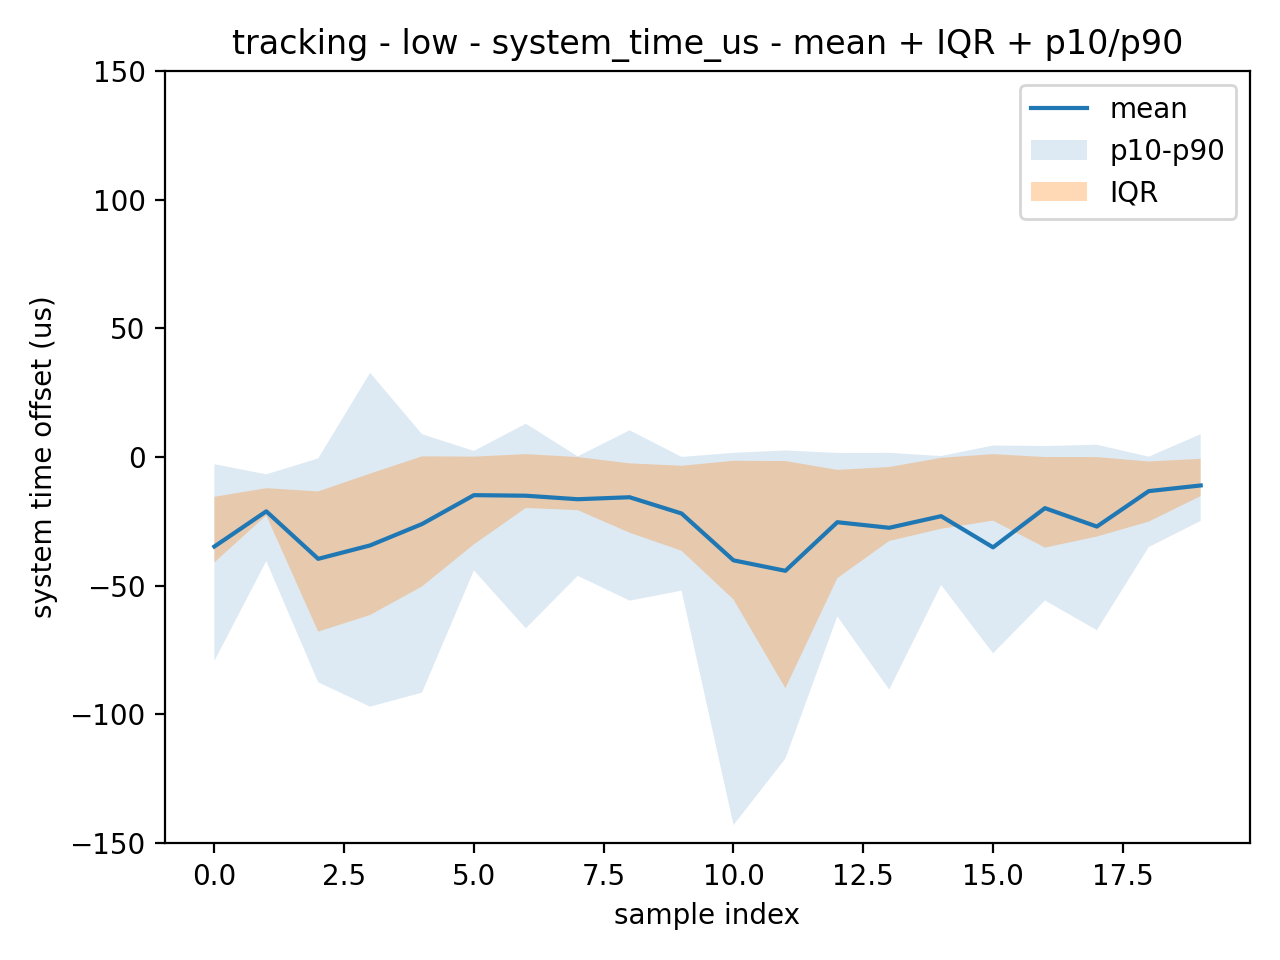
\includegraphics[width=\linewidth]{
      pars_plots/chrony_clientchrony/_aggregated/tracking/low/system_time_us_mean_iqr_p10_p90.png
    }
    \caption{Scenario LOW}
  \end{subfigure}
  \hfill
  \begin{subfigure}
    {0.32\textwidth}
    \centering
    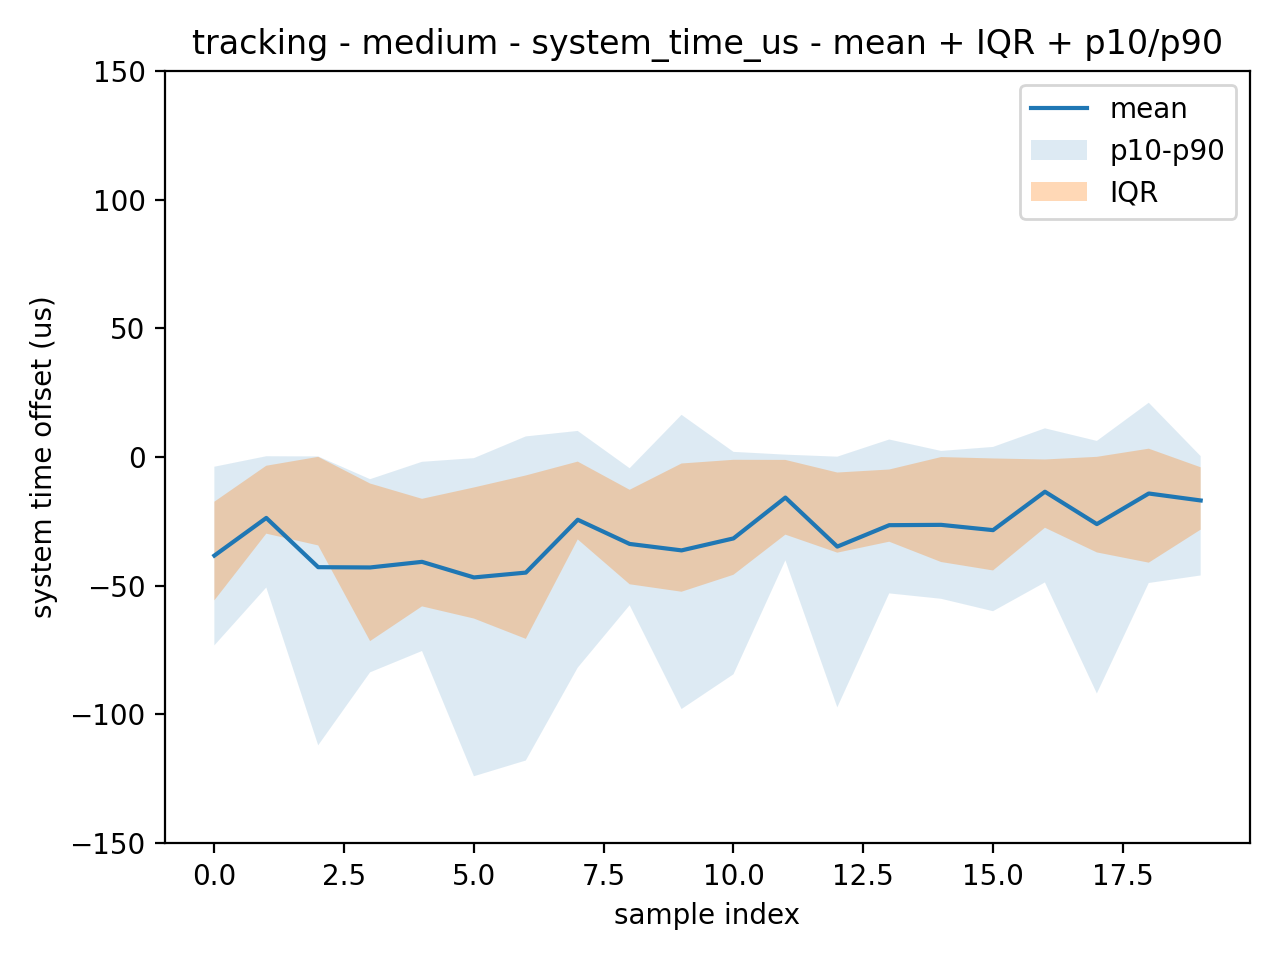
\includegraphics[width=\linewidth]{
      pars_plots/chrony_clientchrony/_aggregated/tracking/medium/system_time_us_mean_iqr_p10_p90.png
    }
    \caption{Scenario MEDIUM}
  \end{subfigure}
  \begin{subfigure}
    {0.32\textwidth}
    \centering
    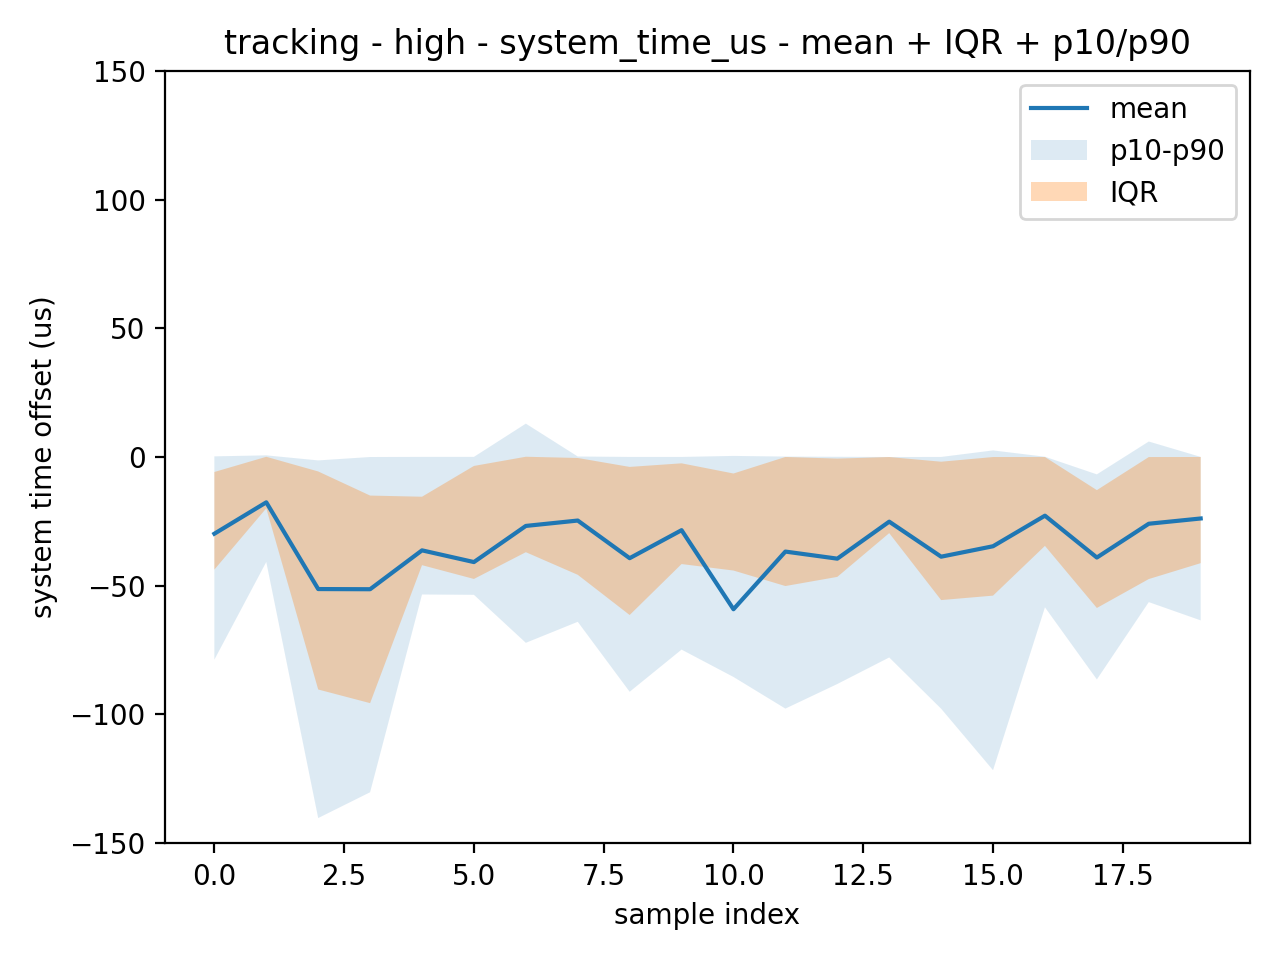
\includegraphics[width=\linewidth]{
      pars_plots/chrony_clientchrony/_aggregated/tracking/high/system_time_us_mean_iqr_p10_p90.png
    }
    \caption{Scenario HIGH}
  \end{subfigure}
  \caption{Media con banda inter-quartile e banda p10-p90 - nodo: \texttt{clientchrony}
  - netem/tc: \texttt{clientchrony}}
  \label{fig:scenario_comparison}
\end{figure}
\paragraph*{clientchrony - netem/tc:}
Nel caso della metrica \texttt{system\_time\_us}, l'analisi relativa a \texttt{clientchrony}
con degrado applicato sul nodo client evidenzia un comportamento più regolare rispetto
ad altre metriche.

Nel caso \texttt{low} la media aggregata è di ~\texttt{-25.284 \,$\mu$s}. La deviazione
standard delle medie è di \texttt{9.885 \,$\mu$s}. I grafici evidenziano oscillazioni
locali. L'IQR medio è pari a \texttt{35.089 \,$\mu$s}. L'ampiezza media dell'intervallo
\texttt{p10-p90} raggiunge \texttt{73.456 \,$\mu$s}, con picchi fino a \texttt{144.596
\,$\mu$s}. Nei dati globali si ha una mediana \texttt{-13.664 \,$\mu$s}, primo quartile
\texttt{-34.557 \,$\mu$s} e terzo quartile \texttt{-0.530 \,$\mu$s}.

Nello scenario \texttt{medium} la media aggregata della curva scende a \texttt{-30.408
\,$\mu$s}. La deviazione standard delle medie pari a \texttt{10.531 \,$\mu$s}. L'IQR
medio vale \texttt{39.129 \,$\mu$s}, mentre l'intervallo medio \texttt{p10-p90} è
\texttt{78.520 \,$\mu$s}. Le statistiche globali hanno mediana \texttt{-22.285 \,$\mu$s}
e quartili pari a \texttt{-46.666 \,$\mu$s} e \texttt{-2.351 \,$\mu$s}.

Nello scenario \texttt{high} la media aggregata della curva è di \texttt{-34.573 \,$\mu$s},
il valore più negativo tra i tre scenari. La deviazione standard delle medie è
\texttt{10.809 \,$\mu$s}. L'IQR medio è \texttt{45.637 \,$\mu$s} e l'ampiezza media
\texttt{p10-p90} è \texttt{82.403 \,$\mu$s}. Si ha mediana pari a\texttt{-19.111 \,$\mu$s},
primo quartile \texttt{-48.642 \,$\mu$s} e terzo quartile \texttt{0.001 \,$\mu$s}.

Nel confronto complessivo tra i tre scenari emerge quindi una dinamica lineare.
Il passaggio da \texttt{low} a \texttt{medium} e poi a \texttt{high} produce infatti
un progressivo spostamento del livello medio verso valori più negativi: \texttt{-25.284
\,$\mu$s}, \texttt{-30.408 \,$\mu$s} e \texttt{-34.573 \,$\mu$s}. La variabilità rimane
ampia in tutti e tre i casi e non cresce in modo altrettanto netto.

\begin{figure}[H]
  \centering

  \begin{subfigure}
    {0.32\textwidth}
    \centering
    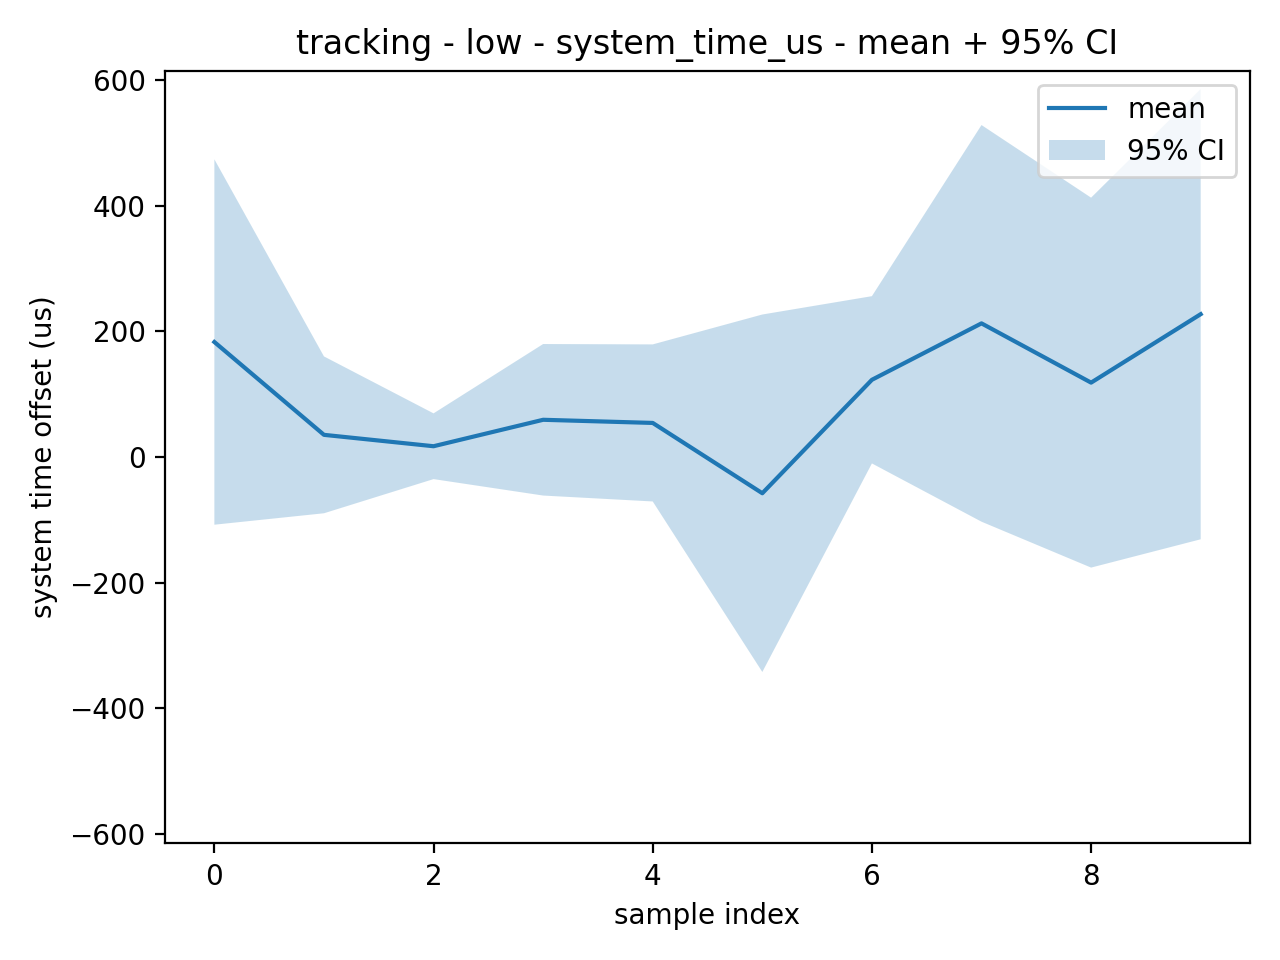
\includegraphics[width=\linewidth]{
      pars_plots/chrony_servergm/_aggregated/tracking/low/system_time_us_mean_ci95.png
    }
    \caption{Scenario LOW}
  \end{subfigure}
  \hfill
  \begin{subfigure}
    {0.32\textwidth}
    \centering
    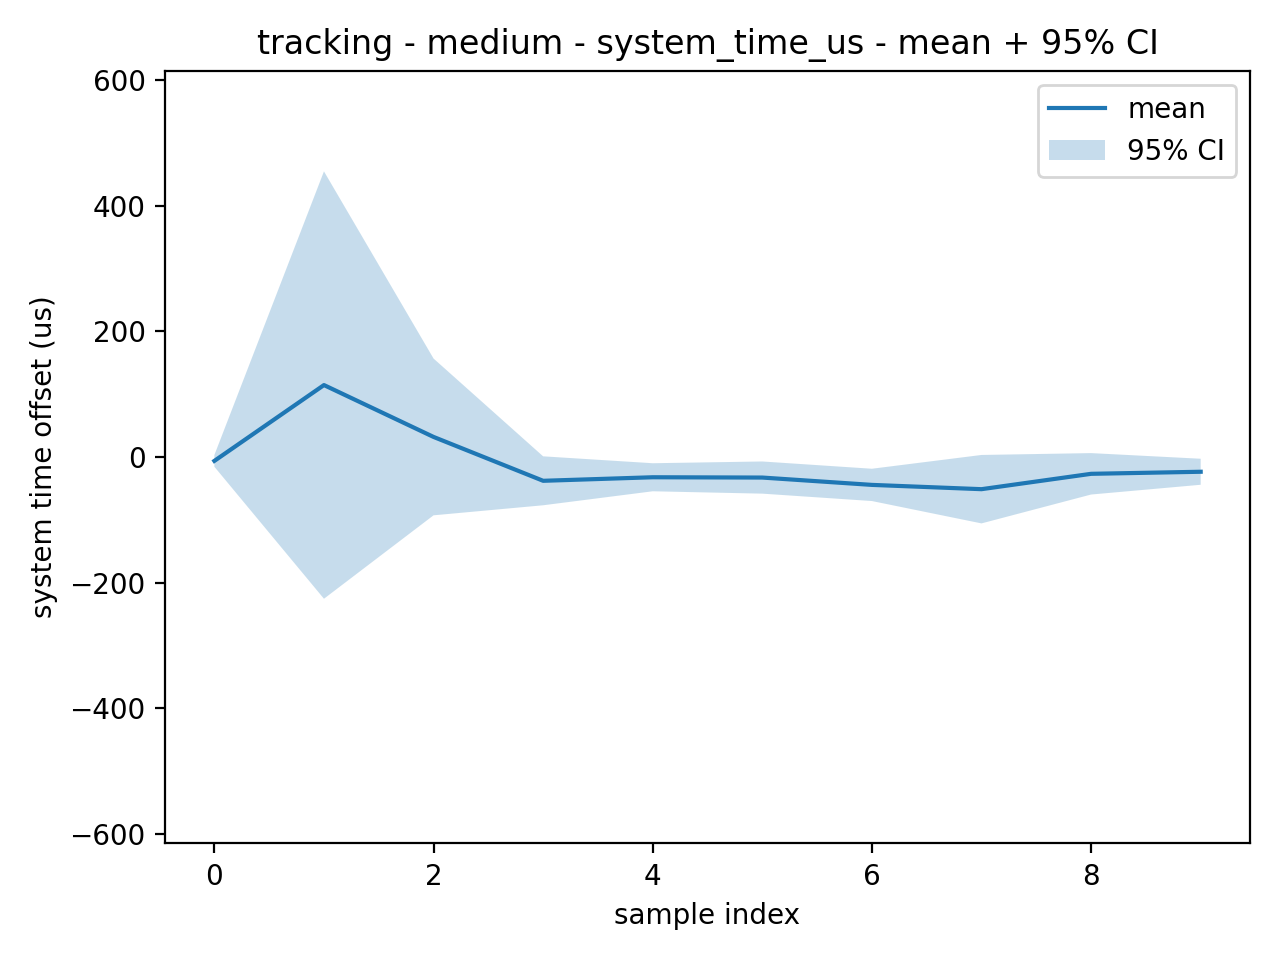
\includegraphics[width=\linewidth]{
      pars_plots/chrony_servergm/_aggregated/tracking/medium/system_time_us_mean_ci95.png
    }
    \caption{Scenario MEDIUM}
  \end{subfigure}
  \begin{subfigure}
    {0.32\textwidth}
    \centering
    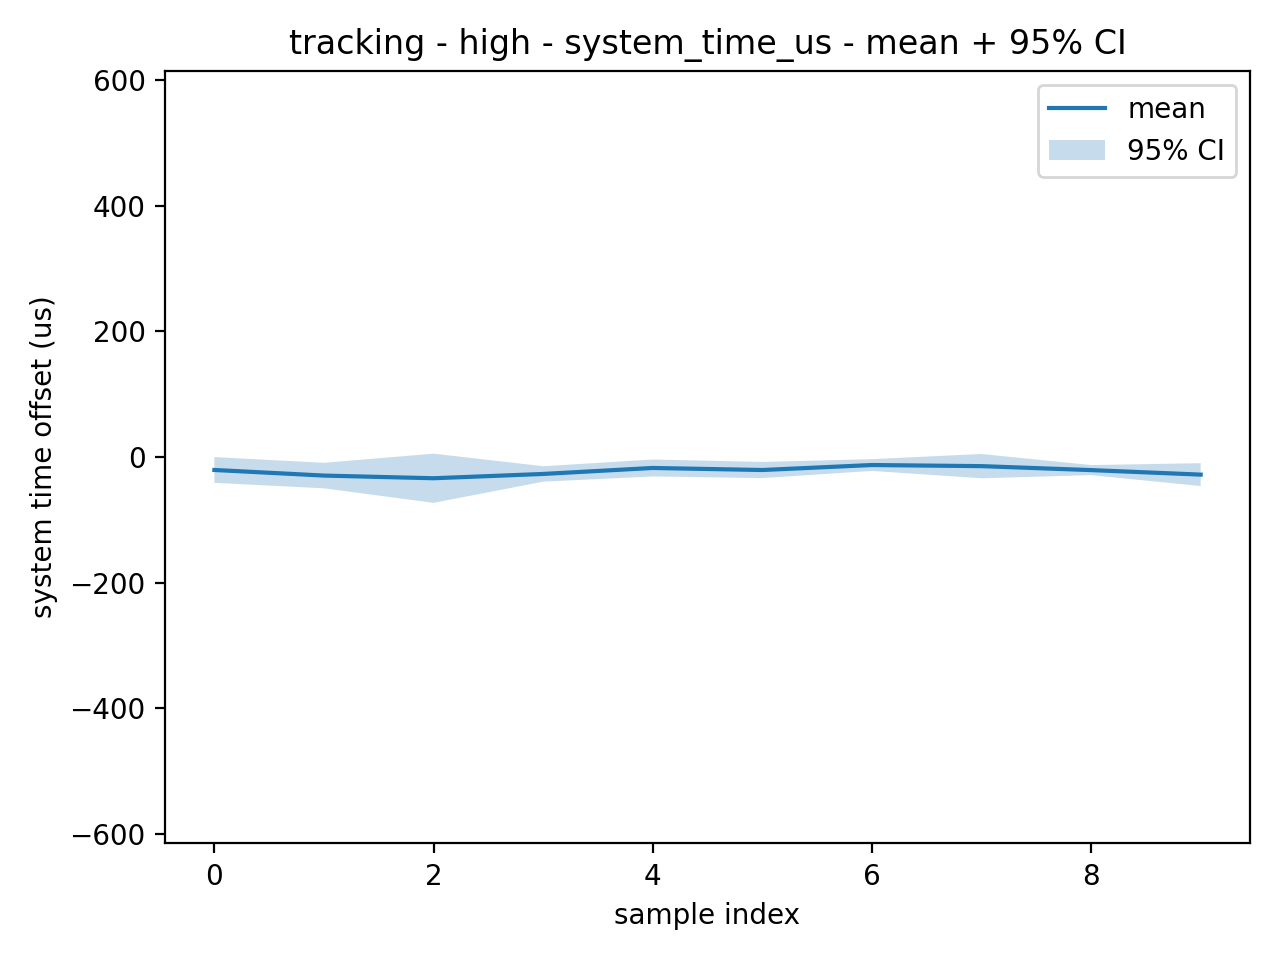
\includegraphics[width=\linewidth]{
      pars_plots/chrony_servergm/_aggregated/tracking/high/system_time_us_mean_ci95.png
    }
    \caption{Scenario HIGH}
  \end{subfigure}
  \caption{Media con intervallo di confidenza al 95\% - nodo: \texttt{clientchrony}
  - netem/tc: \texttt{servergm}}
  \label{fig:scenario_comparison}
\end{figure}
\begin{figure}[H]
  \centering

  \begin{subfigure}
    {0.32\textwidth}
    \centering
    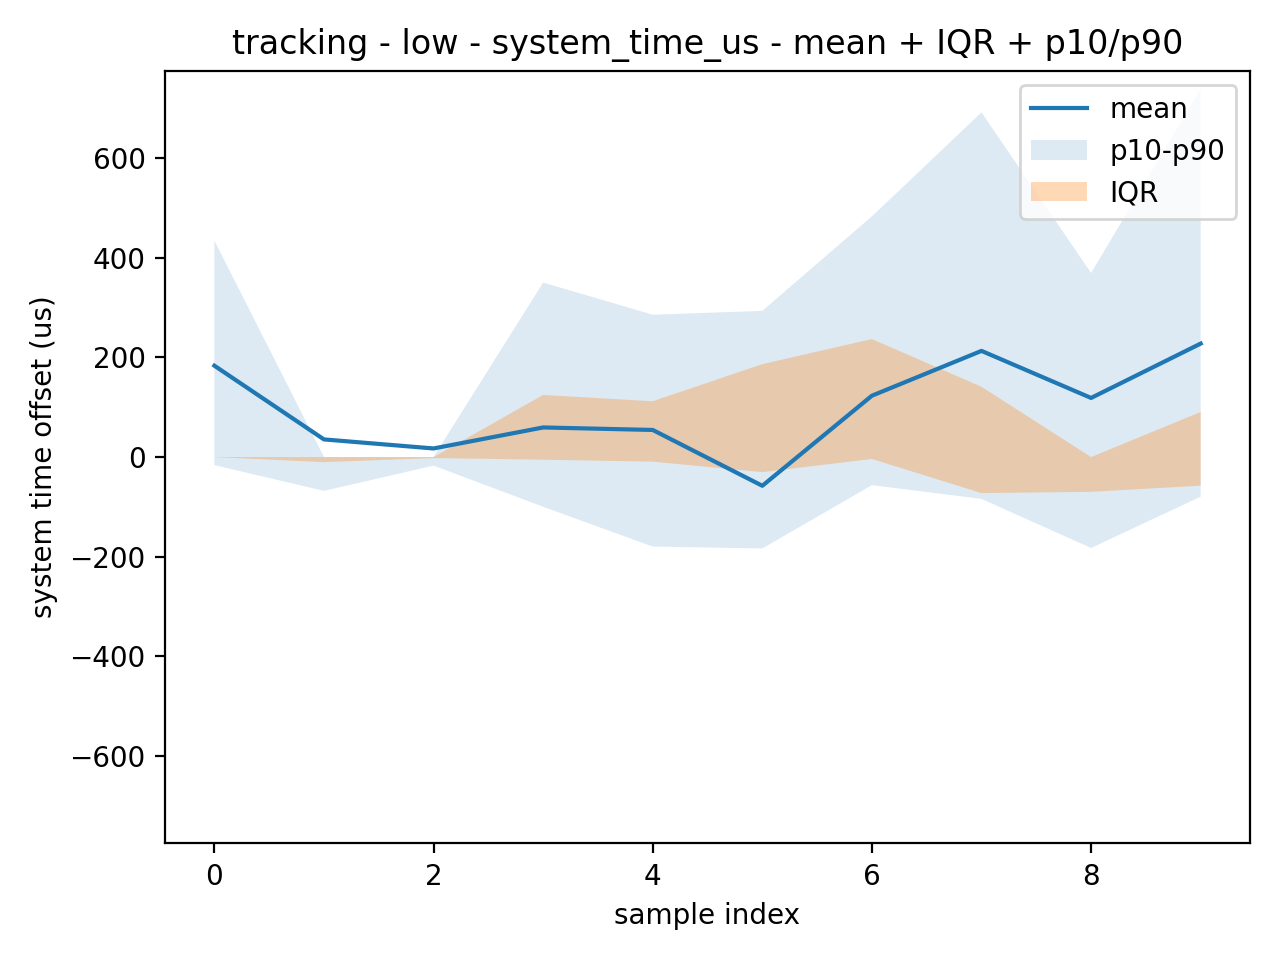
\includegraphics[width=\linewidth]{
      pars_plots/chrony_servergm/_aggregated/tracking/low/system_time_us_mean_iqr_p10_p90.png
    }
    \caption{Scenario LOW}
  \end{subfigure}
  \hfill
  \begin{subfigure}
    {0.32\textwidth}
    \centering
    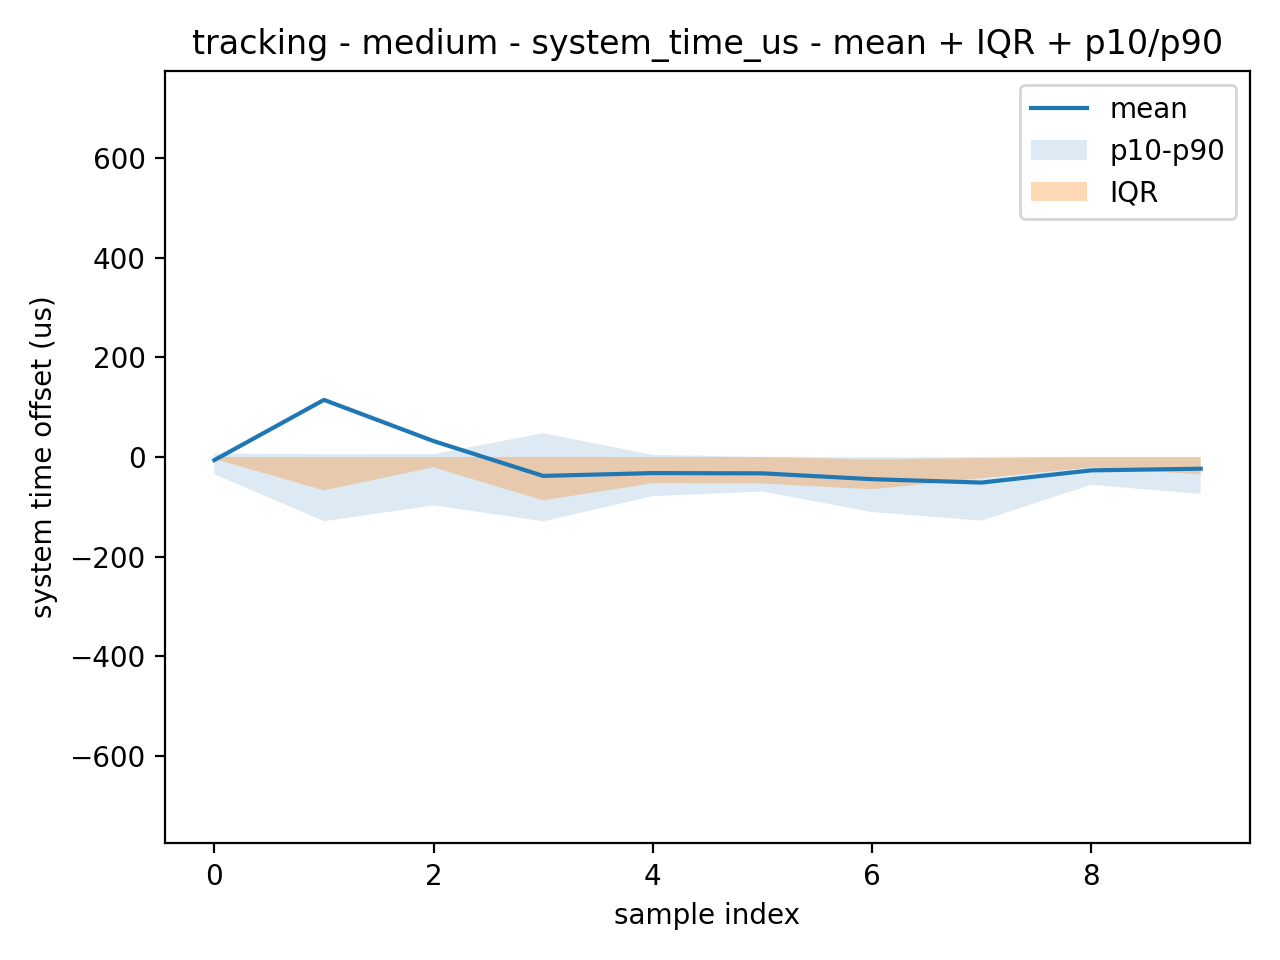
\includegraphics[width=\linewidth]{
      pars_plots/chrony_servergm/_aggregated/tracking/medium/system_time_us_mean_iqr_p10_p90.png
    }
    \caption{Scenario MEDIUM}
  \end{subfigure}
  \begin{subfigure}
    {0.32\textwidth}
    \centering
    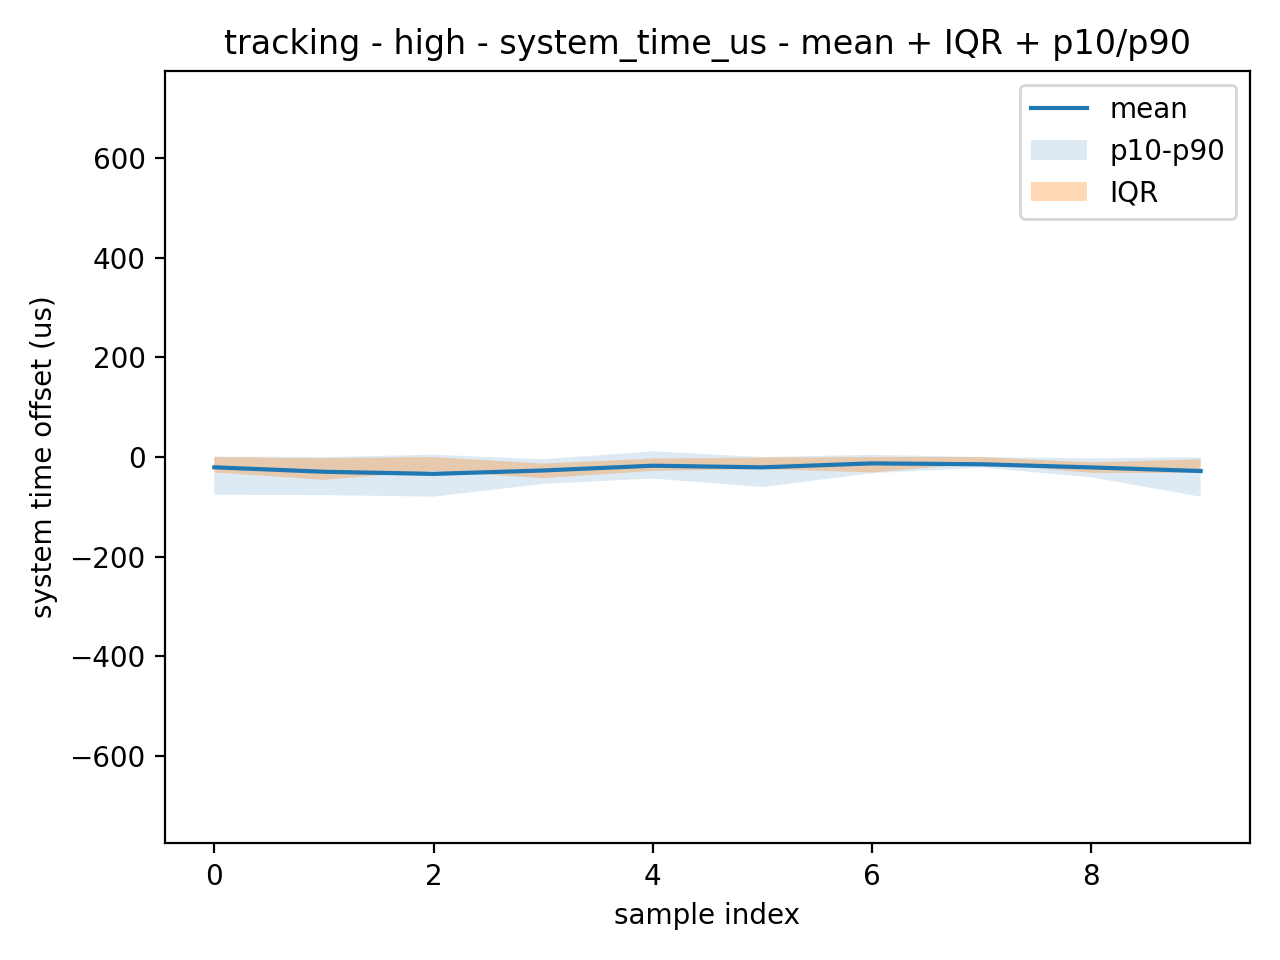
\includegraphics[width=\linewidth]{
      pars_plots/chrony_servergm/_aggregated/tracking/high/system_time_us_mean_iqr_p10_p90.png
    }
    \caption{Scenario HIGH}
  \end{subfigure}
  \caption{Media con banda inter-quartile e banda p10-p90 - nodo: \texttt{clientchrony}
  - netem/tc: \texttt{servergm}}
  \label{fig:scenario_comparison}
\end{figure}

\paragraph*{servergm - netem/tc:}
L'analisi con impairment applicato sul nodo \texttt{servergm} evidenzia un
comportamento fortemente non monotono al variare dello scenario.

Nello scenario \texttt{low}, la metrica assume il livello medio più elevato. La media
aggregata della curva è pari a \texttt{97.407 \,$\mu$s}. La deviazione standard delle
medie pari a \texttt{92.121 \,$\mu$s}. L'IQR medio è \texttt{115.127 \,$\mu$s}, mentre
l'ampiezza media dell'intervallo \texttt{p10-p90} raggiunge \texttt{461.010 \,$\mu$s},
con picchi fino a \texttt{817.440 \,$\mu$s}. Si ha un valore massimo pari a
\texttt{2342.321 \,$\mu$s}.Il caso \texttt{low} descrive quindi una risposta
molto instabile. È evidente la presenza di una media non congrua alle bande inter-quartile
per la maggior parte della run.

Nello scenario \texttt{medium}, la media aggregata della curva scende a \texttt{-10.765
\,$\mu$s}. La deviazione standard delle medie si riduce a \texttt{49.927 \,$\mu$s},
circa la metà del valore osservato nel caso \texttt{low}. L'IQR medio è pari a
\texttt{43.947 \,$\mu$s} e l'intervallo medio \texttt{p10-p90} vale \texttt{97.563
\,$\mu$s}. La mediana è di \texttt{-7.355 \,$\mu$s} e i quartili sono pari a \texttt{-50.338
\,$\mu$s} e \texttt{0.031 \,$\mu$s}.

Nello scenario \texttt{high}, la metrica mostra il comportamento più compatto e regolare.
La media aggregata della curva è pari a \texttt{-22.466 \,$\mu$s}, quindi più
negativa rispetto al caso \texttt{medium}, ma accompagnata da una deviazione
standard delle medie molto contenuta, pari a soli \texttt{6.852 \,$\mu$s}.L'IQR
medio è \texttt{27.040 \,$\mu$s}, mentre l'ampiezza media \texttt{p10-p90} è \texttt{57.641
\,$\mu$s}, entrambe inferiori ai valori osservati negli altri due scenari.

Nel confronto vi è un rapporto non lineare. Lo scenario \texttt{low} è nettamente
il più disperso e presenta anche il livello medio più elevato, positivo e
influenzato da run molto anomale. Lo scenario \texttt{medium} riduce
drasticamente tale effetto. Lo scenario \texttt{high} accentua ulteriormente
questa stabilizzazione. Il degrado applicato sul nodo \texttt{servergm} non
produce un peggioramento progressivo all'aumentare dello scenario

\paragraph*{Confronto:}
Nel confronto tra i due punti di applicazione del degrado non emerge una
superiorità univoca di uno scenario rispetto all'altro.
  \chapter{Discussione dei risultati - Conclusioni}
\label{cha:conclusioni}

  % Conclusions
  %  \input{etc/conclusions.tex}

  \endgroup

  % Bibliography
  \addcontentsline{toc}{chapter}{Bibliografia}
  \printbibliography

  % Attachments
  % \titleformat{\chapter} {\normalfont\Huge\bfseries}{Appendix \thechapter}{1em}{}
  % \appendix
  % \input{attachments/attachment.tex}
\end{document}